%Skript zur Vorlesung "Einführung in die Geophysik 1", Wintersemester 2015/16.
%Prof.Dr. Thomas Bohlen, Geophysikalisches Institut, Fakultät für Physik
%Geschrieben von Julia A.M. Schmid, Sommersemester 2016 




\documentclass[titlepage,numbers=noenddot,headinclude,footinclude=true,cleardoublepage=empty,dottedtoc,BCOR=5mm,paper=a4,fontsize=11pt,ngerman,american,]{report}


\usepackage[utf8]{inputenc}
\usepackage{amsmath}
\usepackage{amssymb}
\usepackage{mathtools}
\usepackage{fontspec}
\usepackage{ngerman}
\usepackage{enumitem}
\usepackage{array}
\usepackage{hyperref}
\usepackage{parskip}
\usepackage{siunitx}
\usepackage{float}
\usepackage{subcaption}


%Erlaubt \marginpar (Notizen am Rand) innerhalb des Mathemodus
\usepackage{marginnote}

%Römische Zahlen
\newcommand{\RM}[1]{\MakeUppercase{\romannumeral #1}}

%Automatischer Abastz nach \itemize
\let\EndItemize\enditemize 
\def\enditemize{\EndItemize\vspace{0.3cm}}

%Automatischer Abastz nach \enumerate
\let\EndEnumerate\endenumerate
\def\endenumerate{\EndEnumerate\vspace{0.3cm}}


%verhindert Abstand bei \underbrace
\newcommand{\ub}[2]{\underbrace{#1}_{\mathclap{#2}}}



%Seitenstil: Kapitel oben auf Seite, Seitenzahlen Rand außen
\usepackage{fancyhdr}
\pagestyle{fancy}
\fancyhead{} % clear all header fields
\fancyhead[LE,RO]{\slshape \rightmark}
\fancyfoot{} % clear all footer fields
\fancyfoot[LE,RO]{\thepage}

\begin{document}

%Titelseite mit offiziellem KIT Logo
\begin{titlepage}
	\centering
	\includegraphics{Deckblatt/LogoKIT}
 	\vspace{1.5cm} \par
	{\huge\bfseries Einführung in die Geophysik \RM{1} \par}
	\vspace{2cm}
	{\Large Prof. Dr. Thomas Bohlen\par}
	\vspace{1cm}
	
	{\large Wintersemester 2015/16}
	\vfill
	\par

	\vfill

% Bottom of the page
	{\large Fakultät für Physik \par}
\end{titlepage}



	\tableofcontents

	\chapter{Was ist Geophysik?}

Geophysik bedeutet "`Physik der Erde"' und beschäftigt sich mit den Eigenschaften und physikalischen Vorgängen in unserer Erde. Die Erforschung des Untergrunds erfolgt durch lokale geophysikalische Messungen an der Erdoberfläche. 

 Als Teilgebiete der Geowissenschaften und der Physik umfasst die Geophysik sehr viele Bereiche und hat viele Einsatzgebiete:
 
\vspace{0.7cm}
 
\begin{tabular}{ll}
  \textbf{Tiefenbereich} & \textbf{Anwendung}\\
  0 -- 50\,m & Ingenieurgeophysik (Baugrund, Grundwasser, Deponien \dots )\\
  < 5\,km & Exploration und Speicherung (Erdöl, Erdgas, $\text{CO}_2$, \dots )\\
  < 30 -- 40\,km & Tektonik (Plattentektonik, Krustenstruktur)\\
  < 6371\,km & Aufbau der globalen Erde
\end{tabular} 

In dieser Vorlesung werden wir verschiedene Messmethoden für geophysikalische Messungen zur Untersuchung in allen Tiefenbereichen kennen lernen.
 
\section{Arbeitsmethodik}
Wir wollen uns einmal anschauen, wie eine geophysikalische Untersuchung, unabhängig von der Messmethode, abläuft. \par

Am Anfang einer geophysikalischen Untersuchung steht eine Hypothese zur Struktur des Untergrundes. Anhand dieser Hypothese und mit Hilfe physikalischer Theorie lassen sich Messwerte vorhersagen. Diesen Prozess bezeichnet man als \textbf{Vorwärtsmodellierung}.

Der nächste Schritt ist die \textbf{Beobachtung}. Es wird eine geeignete Messmethode gewählt und durch Beobachtung der entsprechenden Messgröße an der Erdoberfläche werden Daten zur Struktur des Untergrundes gesammelt und anschließend bereinigt. 

Sind die Daten gesammelt und bereinigt, beginnt die Interpretation und \textbf{Inversion}. Durch systematisches Verändern der Hypothese des Untergrundmodells werden die hypothetischen Daten den tatsächlichen angepasst. Dabei ist zu beachten, dass es in der Regel mehrere Untergrundmodelle mit gleichen oder ähnlichen Messwerten gibt, was unter dem Begriff \textbf{Mehrdeutigkeit} bekannt ist. 

Am Ende dieses Prozesses steht ein physikalisches Modell des Untergrunds. 

Bei einem Großteil der Messungen lässt sich das Untersuchungsobjekt einfach isolieren, d.h. Lokalisierung und Größe sind leicht herauszufinden. Bei manchen Untersuchungsobjekten, wie z.B. dem Erdkern, ist dies allerdings nicht möglich. Man spricht dann von einer \textbf{komplexen Struktur}.   


	\chapter{Seismik}

Das Gebiet der Seismik umfasst die Analyse der Ausbreitung elastischer Wellen in der Erde. Diese Wellen werden an Schichtgrenzen oder Objekten im Untergrund reflektiert, refraktiert und transmittiert. Was genau das bedeutet, wollen wir nach einer Einführung in das Thema seismische Wellen klären.  

\section{Seismische Wellen} 
Man unterscheidet zwischen zwei verschiedenen Wellentypen, den Raum- und den Oberflächenwellen. 
\subsection{Raumwellen}
Raumwellen breiten sich über einen Raum aus, das heißt in unserem Fall, dass sie bis weit unter die Erdoberfläche über einen großen Bereich wirken.

\subsubsection{P-Welle}
Eine P-Welle schwingt parallel zur Ausbreitungsrichtung und ist damit eine Kompressionswelle (Longitudinalwelle). P-Welle ist hierbei die Abkürzung für Primär-Welle, da diese Welle die schnellste Wellenart ist und somit als erstes auftritt.
 
\subsubsection{S-Welle} 
Die S-Welle ist langsamer als die P-Welle und tritt als zweites auf. Daher auch der Name Sekundär-Welle. Es handelt sich bei der S-Welle um eine Scherwelle (Transversalwelle) und der Ausschlag ist senkrecht zur Ausbreitungsrichtung. In Flüssigkeiten treten S-Wellen nicht auf.

\begin{figure}[H]
	\begin{subfigure}[m]{0.5\textwidth}
		\centering
		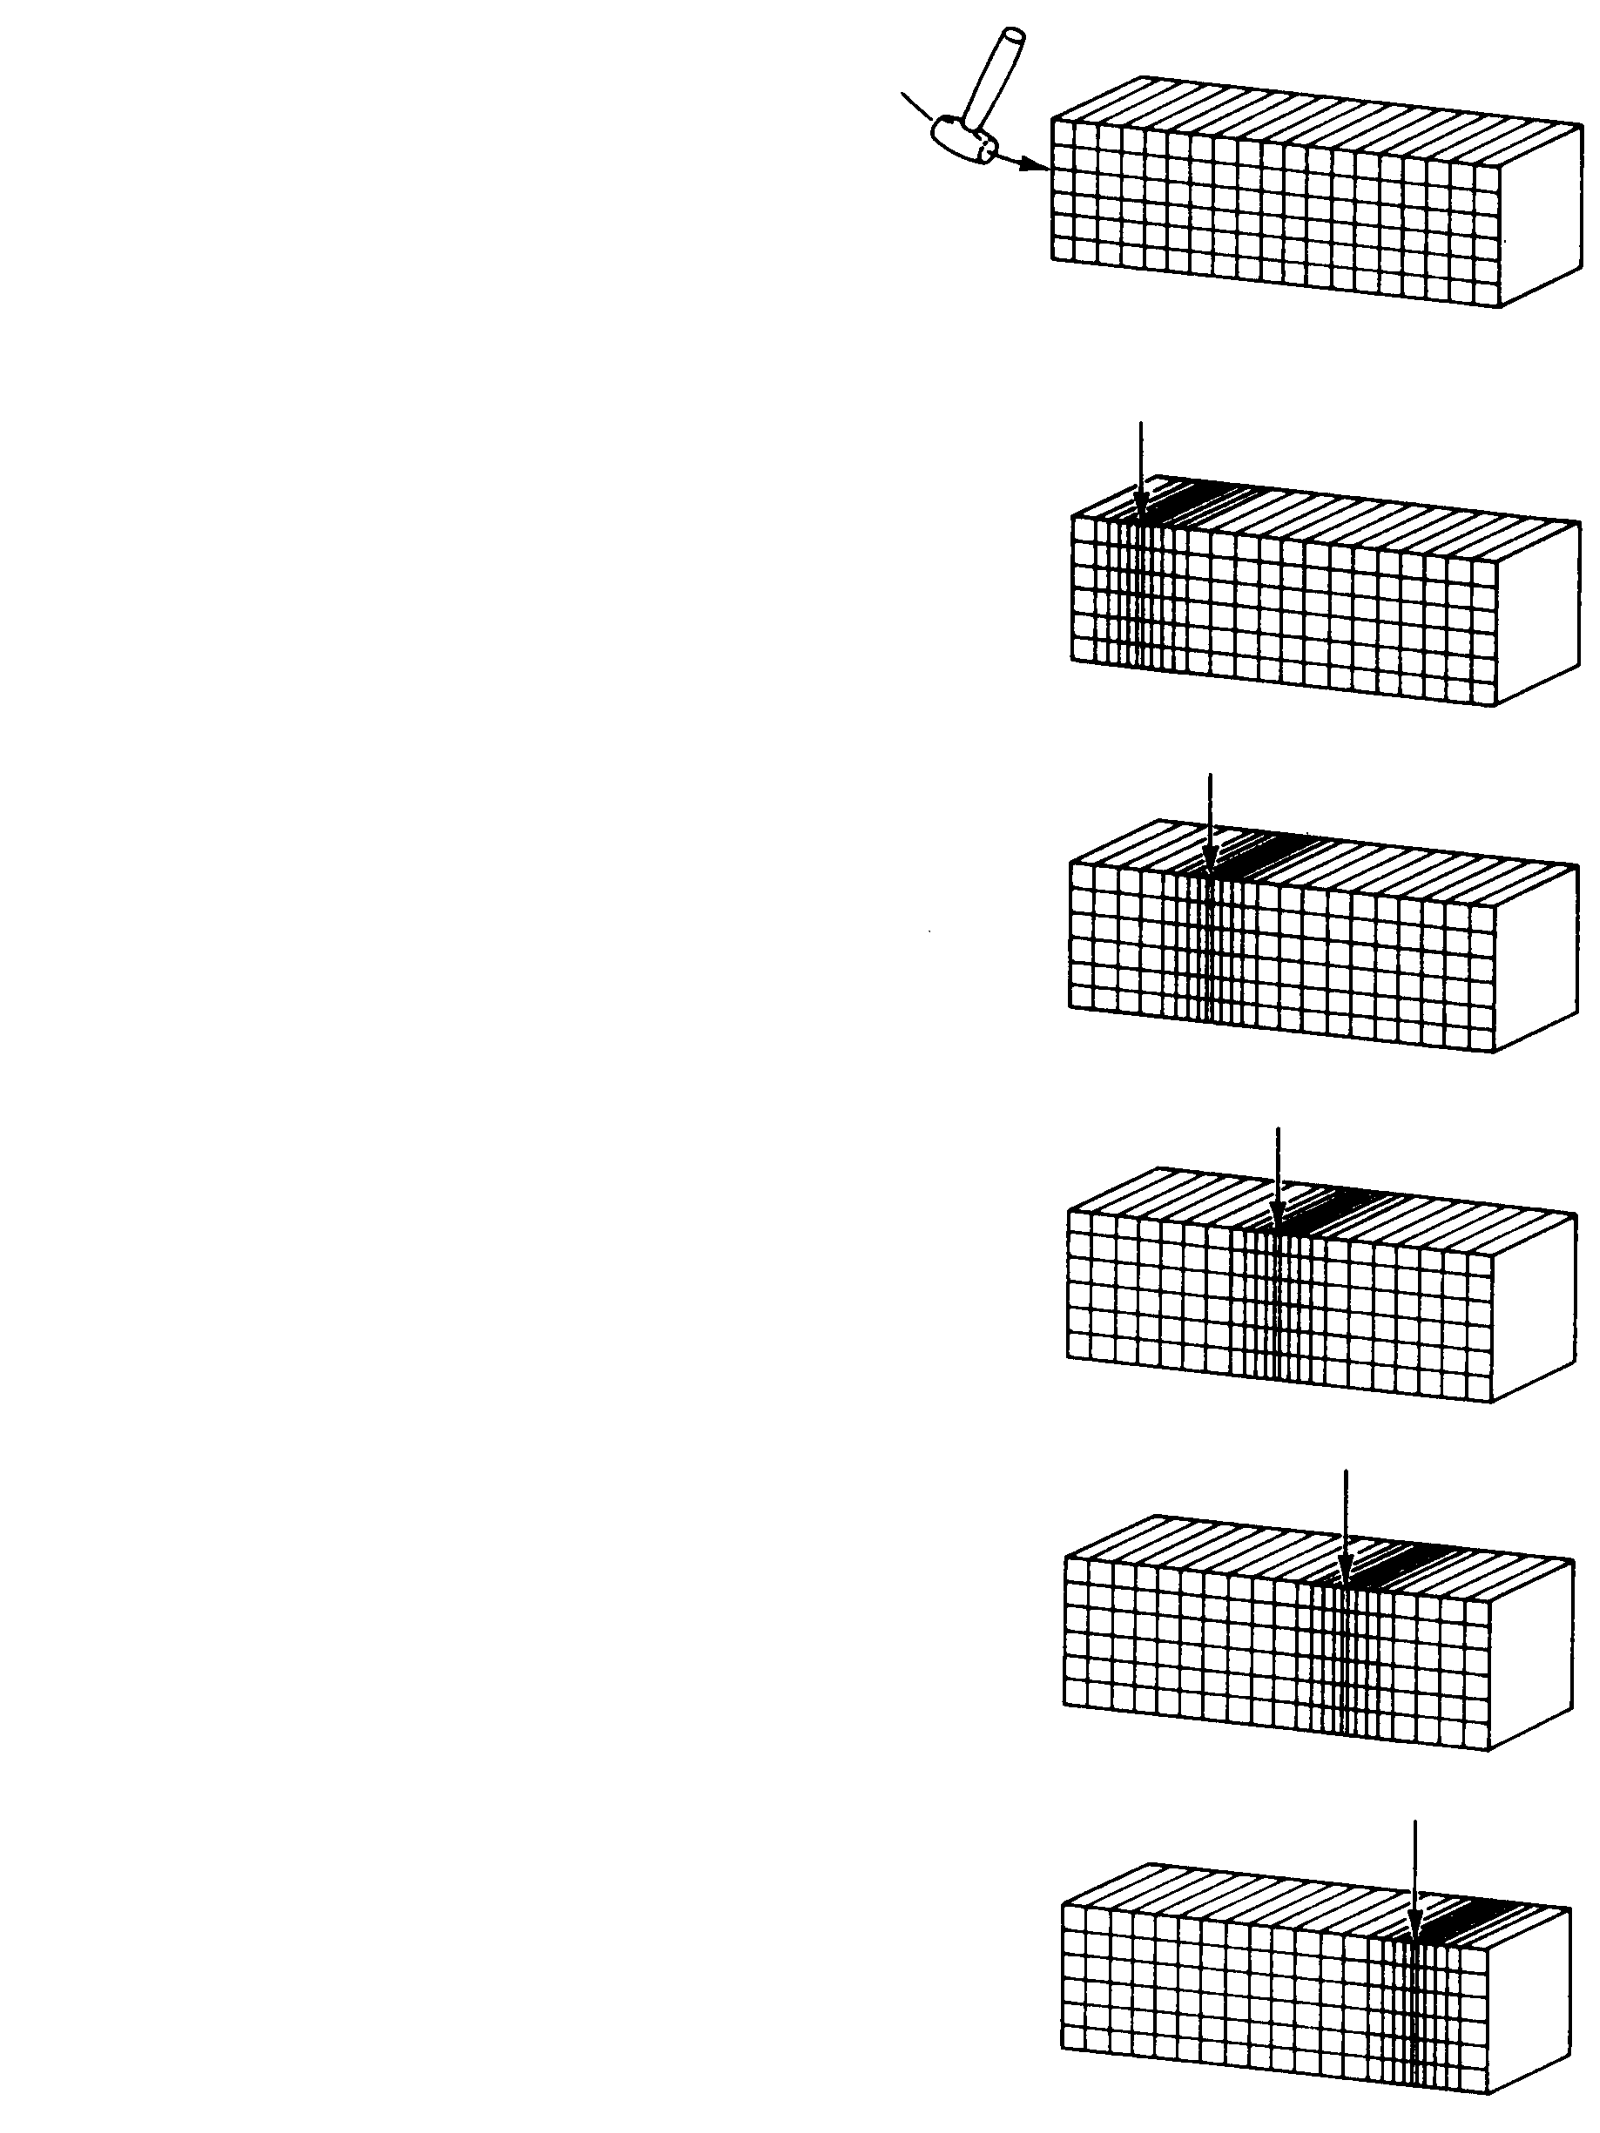
\includegraphics[scale = 0.3]{SeismikBilder/PWelle}
		\caption*{P-Welle}
	\end{subfigure}
	\begin{subfigure}[m]{0.5\textwidth}
		\centering
		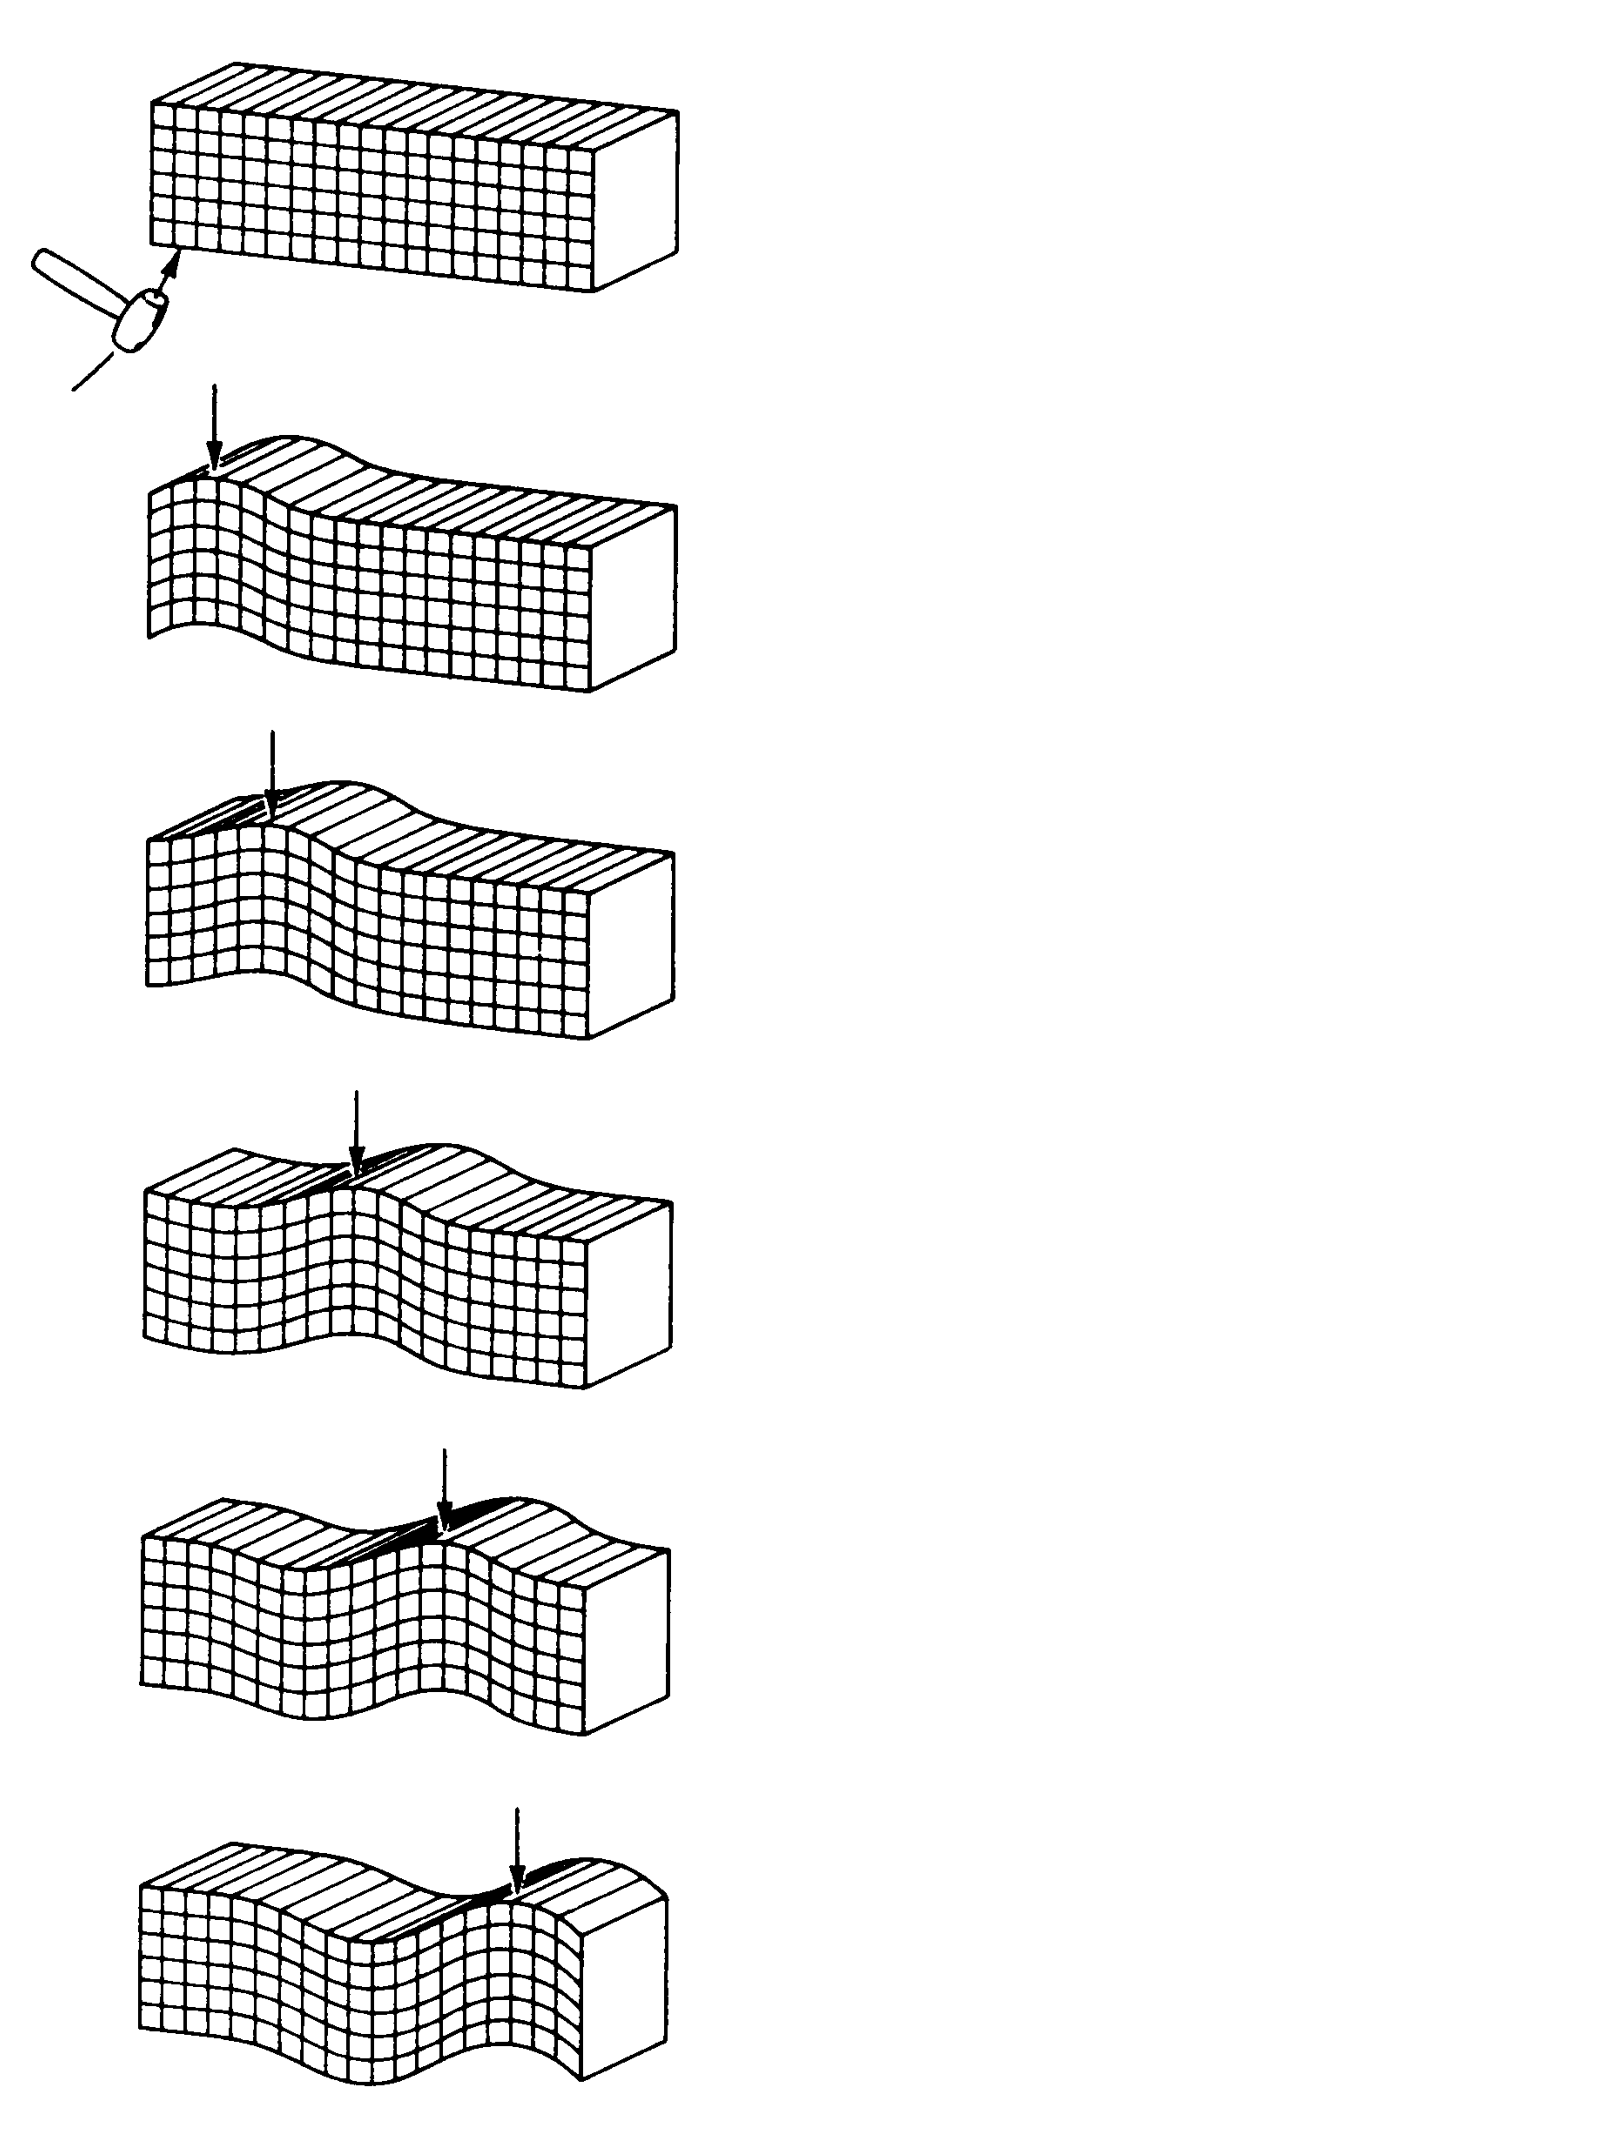
\includegraphics[scale = 0.3]{SeismikBilder/SWelle}
		\caption*{S-Welle}
	\end{subfigure}
\end{figure}

\subsection{Oberflächenwellen}
Wie der Name schon sagt, wirken diese Wellen an der Oberfläche. Allerdings wirken auch sie bis weit in die Tiefe. Die Amplitude, also die Stärke der Welle, nimmt jedoch mit der Tiefe exponentiell ab. 

\subsubsection{Rayleigh-Welle}
Die Rayleigh-Welle ist eine Mischung aus P- und S-Welle, weshalb die Bodenbewegung elliptisch ist. Ist die Bewegung im Uhrzeigersinn, spricht man von retrograder Bewegung, bei Gegenuhrzeigersinn von prograder Bewegung.

Trotz exponentieller Abnahme der Amplitude sind bei starken Erdbeben Schwingungen bis zum Erdkern möglich.


\begin{figure}[H]
	\begin{subfigure}[m]{0.5\textwidth}
		\centering
		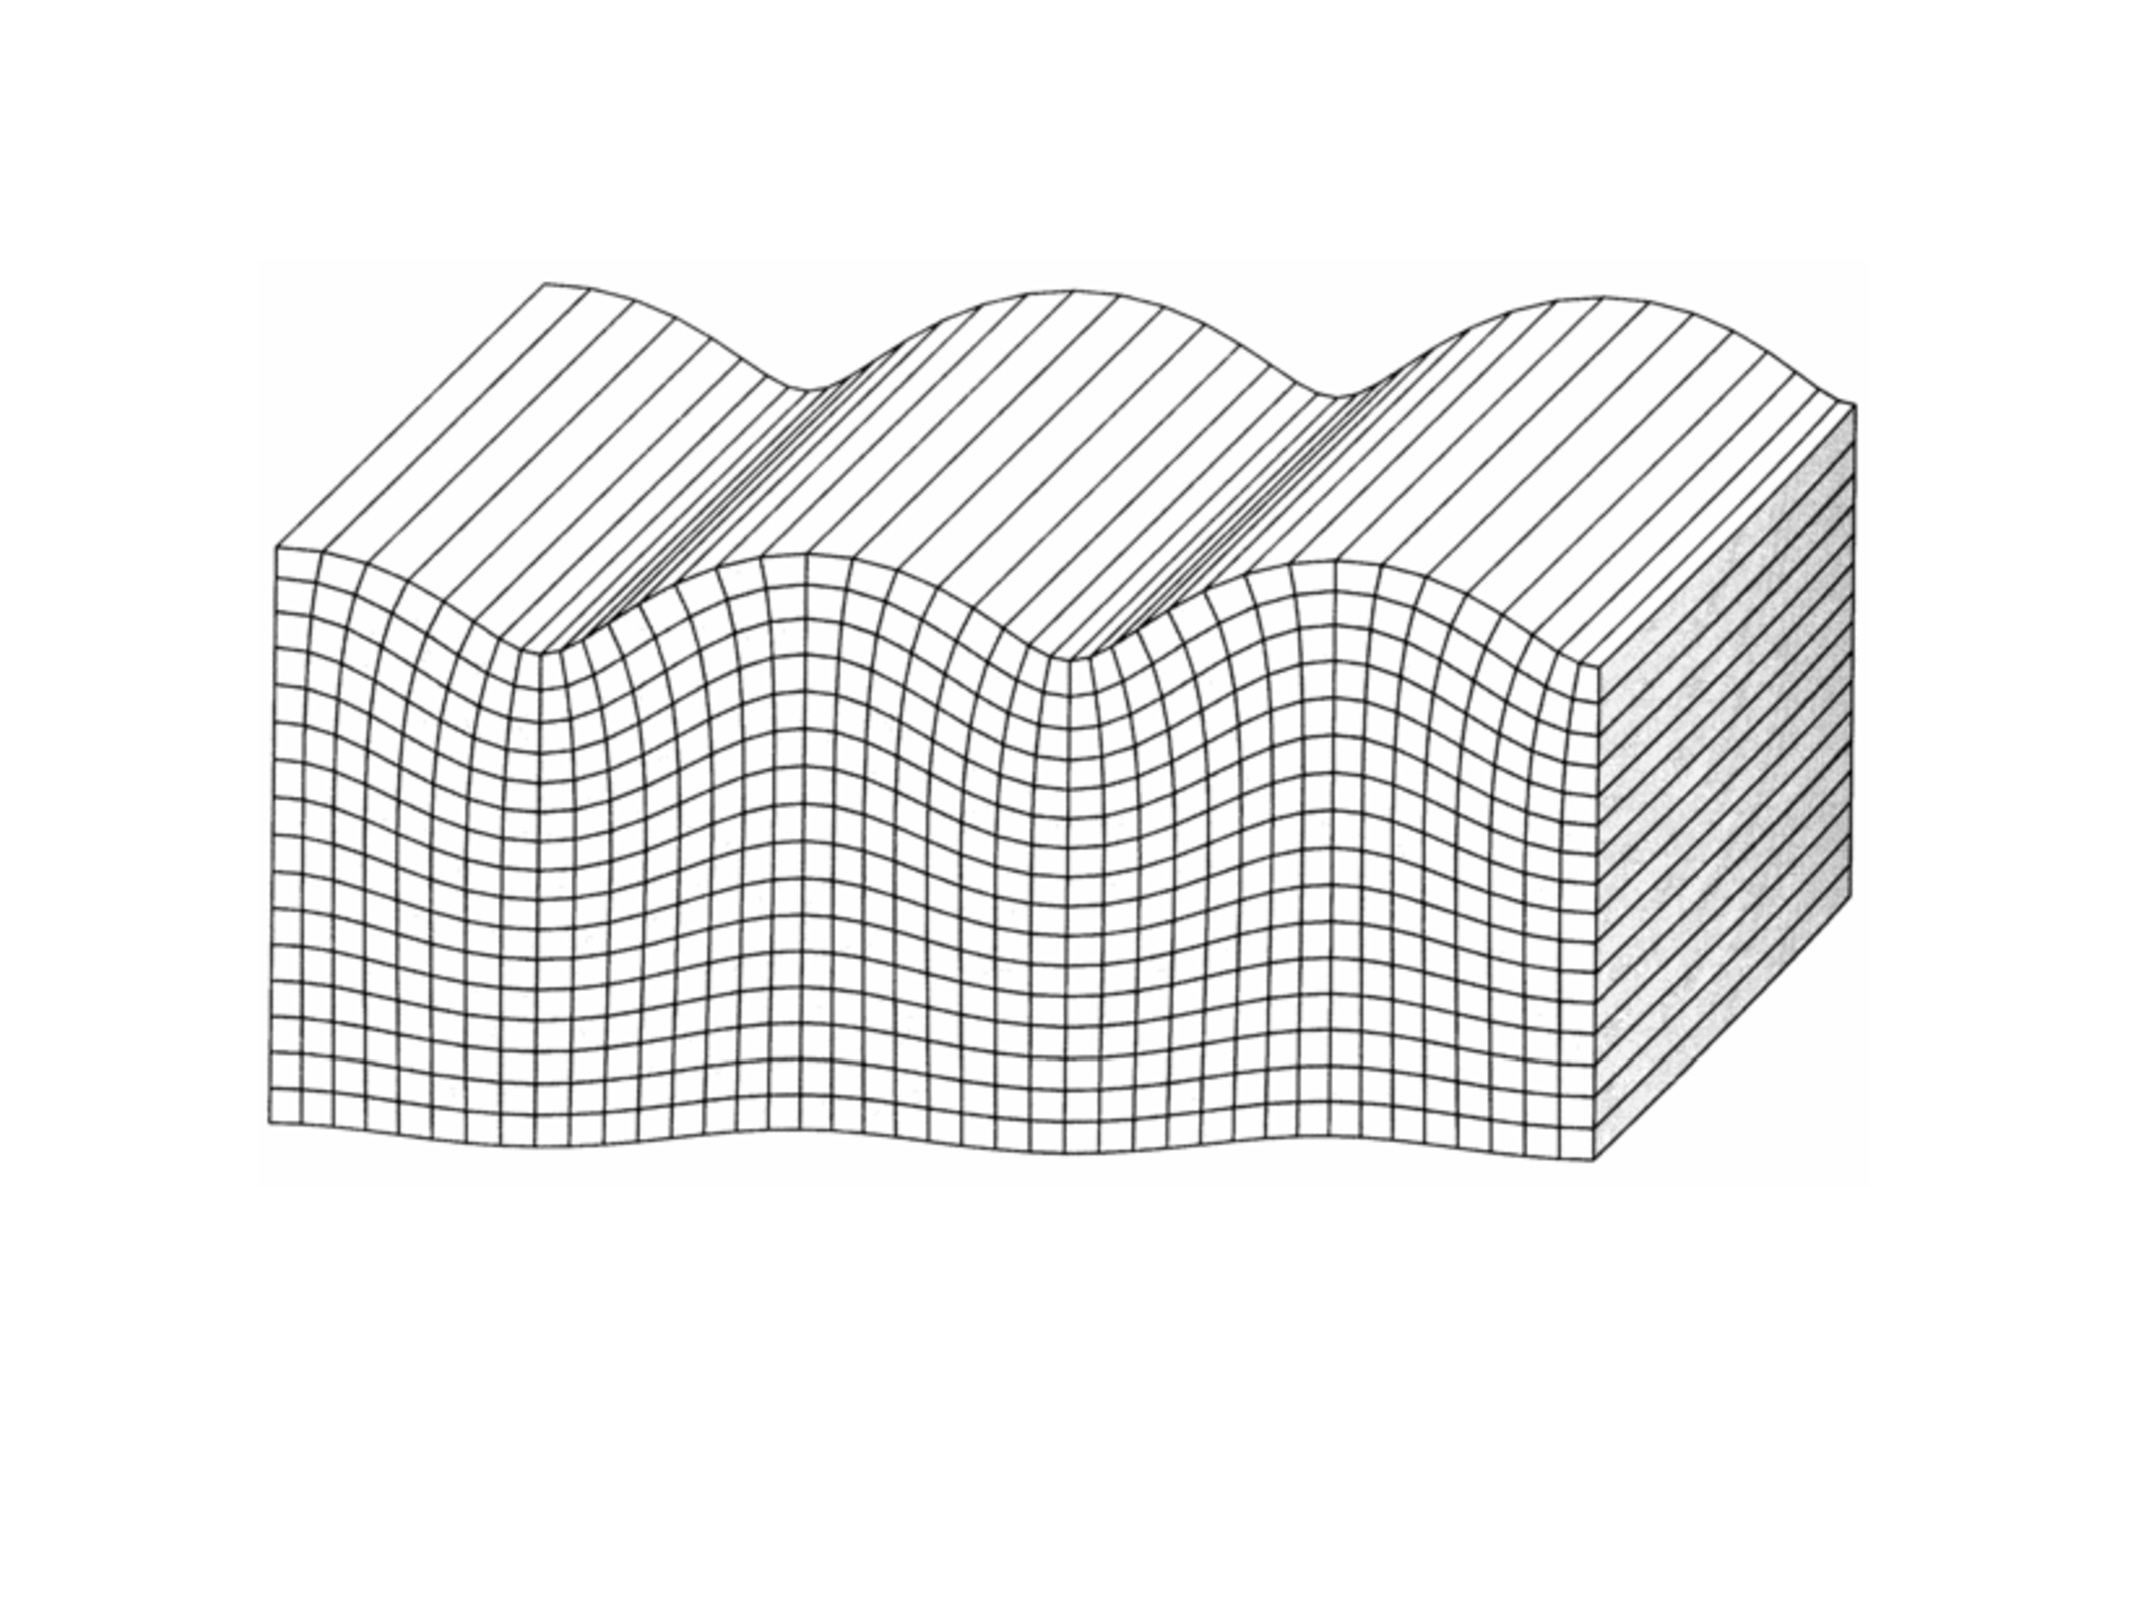
\includegraphics[scale = 0.2]{SeismikBilder/RayleighWelle}
	\end{subfigure}
	\begin{subfigure}[m]{0.5\textwidth}
		\centering
		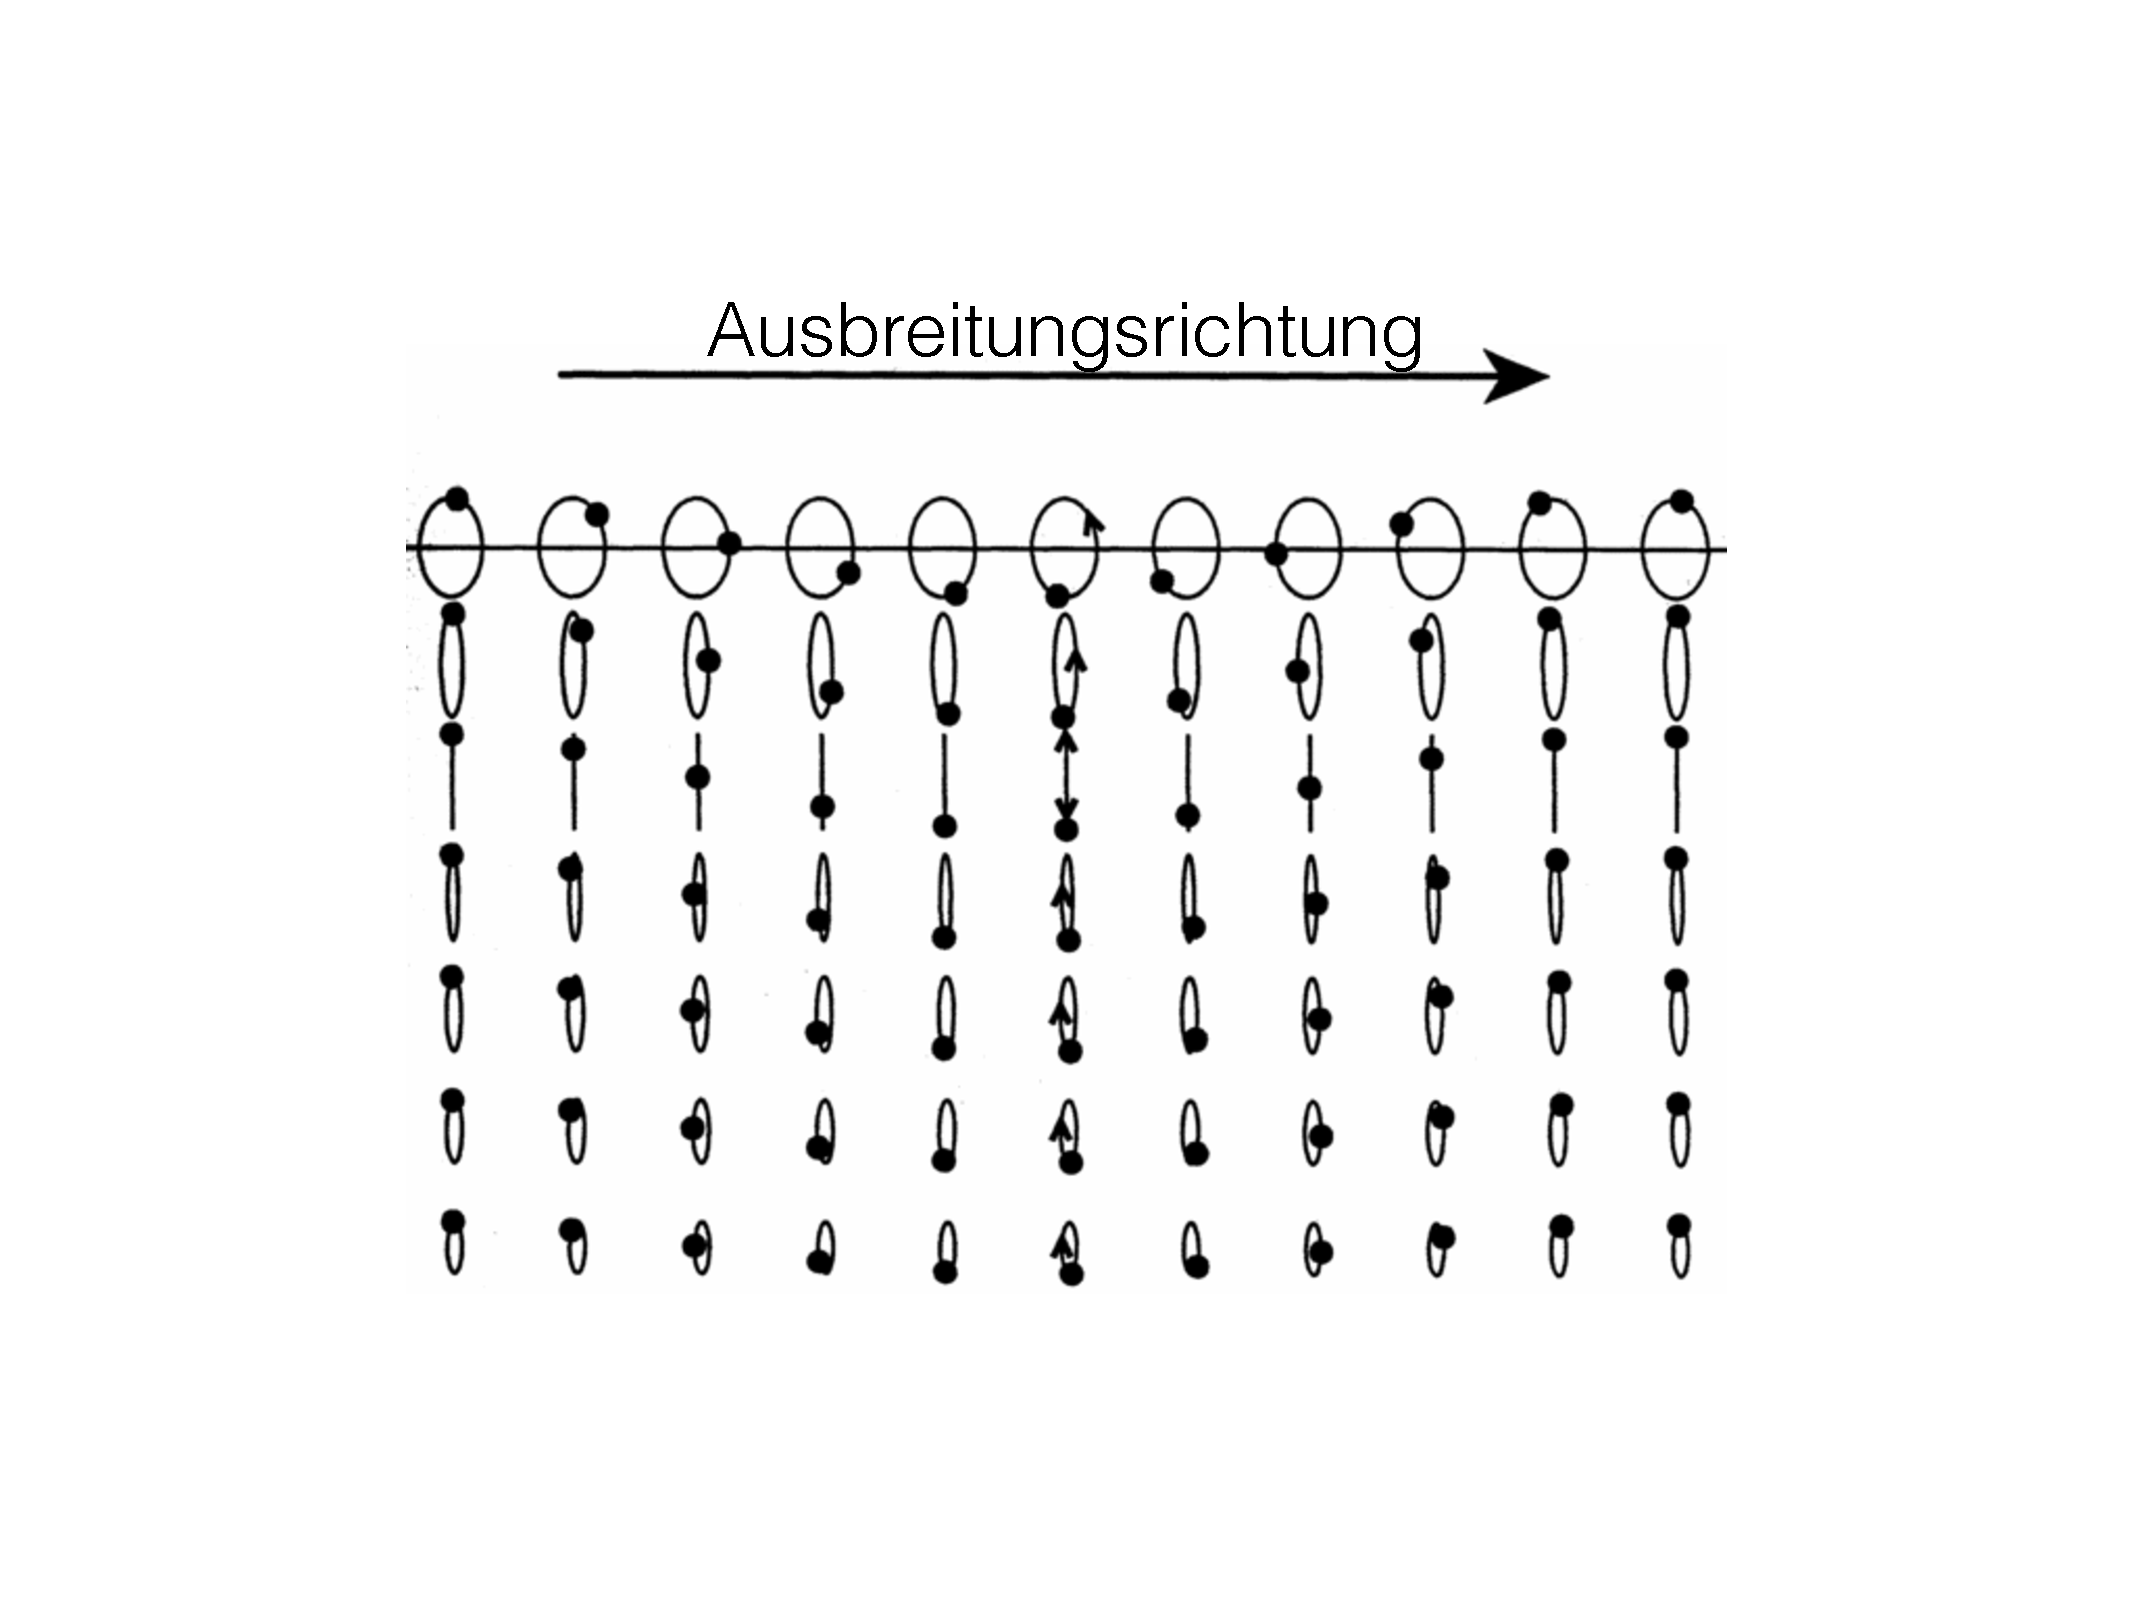
\includegraphics[scale = 0.2]{SeismikBilder/BodenbewegungRayleigh}
	\end{subfigure}
	\caption*{Bodenbewegung einer Rayleigh-Welle \textsl{Quelle: Shearer}}
\end{figure}

\subsubsection{Love-Welle}
Eine Love-Welle ist eine S-Welle mit Schwingungsrichtung parallel zur Erdoberfläche.

\begin{figure}[H]
	\centering
	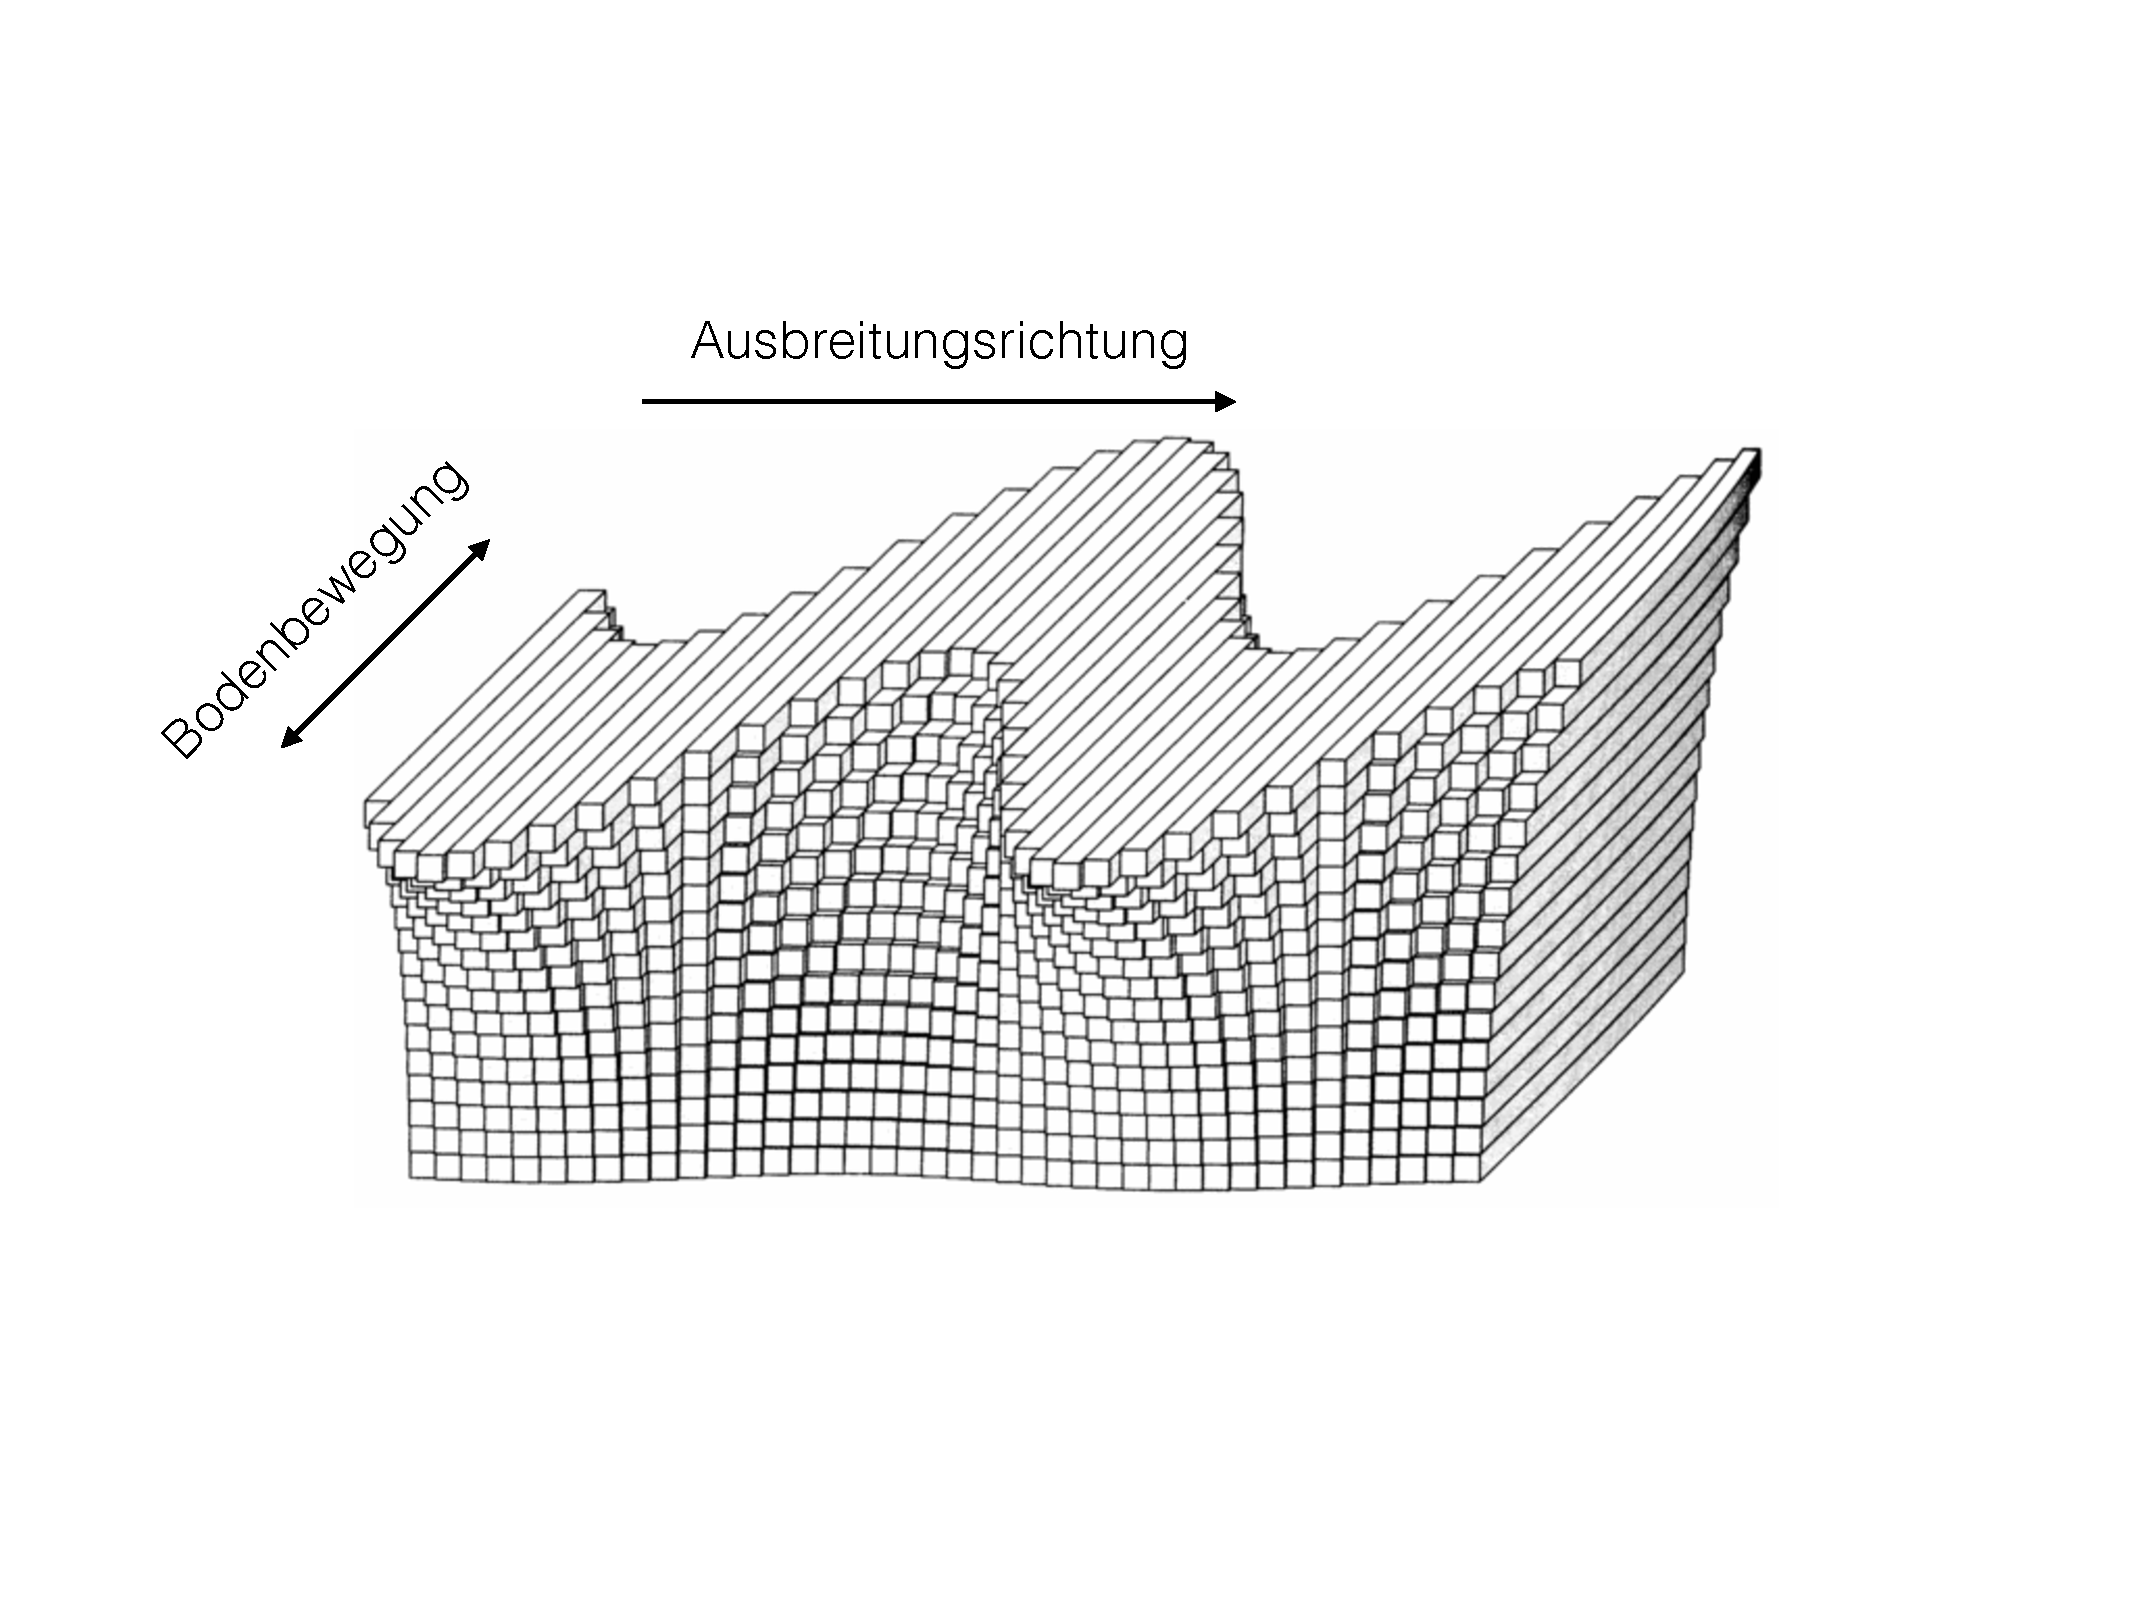
\includegraphics[width = \textwidth]{SeismikBilder/LoveWelle}
	\caption*{\textsl{Quelle: Shearer}}
\end{figure}


\section{Ausbreitungsgeschwindigkeiten}
Die Geschwindigkeiten der Wellen sind abhängig von den elastischen Moduln. Diese Moduln sind Konstanten, die abhängig von den Eigenschaften des Materials sind.
Uns interessieren dabei besonders zwei davon: \begin{description}
	\item[Kompressionsmodul $K$:] Dieser Wert gibt an, wie stark man einen Körper zusammendrücken muss, bis er sein Volumen verändert.
	\item[Schermodul $\mu$:] Der Wert des Schermoduls gibt den Widerstand des Materials gegen Scherkräfte an.\end{description}

Beide Werte werden in Pascal (\si{Pa}) angegeben.


Um die Wellengeschwindigkeit von P- und S-Welle berechnen zu können, müssen die elastischen Moduln $K$ und $\mu$, sowie die Dichte $\rho$ des Untergrunds bekannt sein.

\subsection{Geschwindigkeit P-Welle}
\begin{equation*}
	v_{\text{p}} = \sqrt{\frac{K + \frac{4}{3} \mu}{\rho}}
\end{equation*}
Ein wichtiger Faktor für die Geschwindigkeit einer P-Welle ist der Sättigungsgrad der Poren mit Wasser. Ab einem Sättigungsgrad von 85\% steigt die Geschwindigkeit stark an.

\subsection{Geschwindigkeit S-Welle}
\begin{equation*}
	v_{\text{s}} = \sqrt{\frac{\mu}{\rho}}
\end{equation*}
In Flüssigkeiten gilt $\mu = 0$, da S-Wellen hier nicht auftreten. \par

Um ein Gefühl für die Geschwindigkeit einer Bodenwelle zu bekommen seien hier Werte einer P-Welle genannt. 

\begin{tabular}{ll}
	\textbf{Material} & \textbf{Typische Geschwindigkeit}\\
	Luft & 0,33\,\si{km/s} \\
	Sand, Verwitterungsboden & 0,3 -- 1,5 \si{km/s} \\
	Wasser & 1,5\,\si{km/s}\\
	Eis & 3,0 -- 4,0\,\si{km/s}\\
	Sandstein & 1,5 -- 4,3\,\si{km/s}\\
	Kalkstein/Dolomit & 4,0 -- 4,5\,\si{km/s}\\
	Steinsalz & 4,0 -- 5,5\,\si{km/s}\\
	Granit & 5,8 -- 6,2\,\si{km/s}\\
	Gabbro & 6,4 -- 7,6\,\si{km/s}\\
	Peridotit & 7,8 -- 8,4\,\si{km/s}
\end{tabular}

\subsection{Poisson-Zahl}
Die Poisson-Zahl $\sigma$ beschreibt das Verhältnis der Quer- zur Längsverformung. Dieses Verhältnis erlaubt Aussagen über das Verhalten einer Materie bei Belastung in eine Richtung. Bei einer Flüssigkeit beispielsweise bleibt das Volumen bei Quetschung erhalten, da die Flüssigkeit einfach zur Seite ausweicht. $\sigma$ ist in diesem Fall 0,5. Dies ist der höchste Wert, den die Poisson-Zahl annehmen kann. Eine Flüssigkeit ist demnach ideal plastisch.
Festkörper können bei Quetschung und Dehnung aufgrund ihrer elastischen Eigenschaften nicht instantan reagieren und zur Seite ausweichen. $\sigma$ ist hier im Bereich um 0,25. Besonders ist $\sigma$ von Quarz. Hier beobachtet man eine negative Poisson-Zahl. Das liegt daran, dass Quarz sich lateral zusammenzieht wenn eine axiale Spannung anliegt.

\begin{figure}[H]
	\centering
	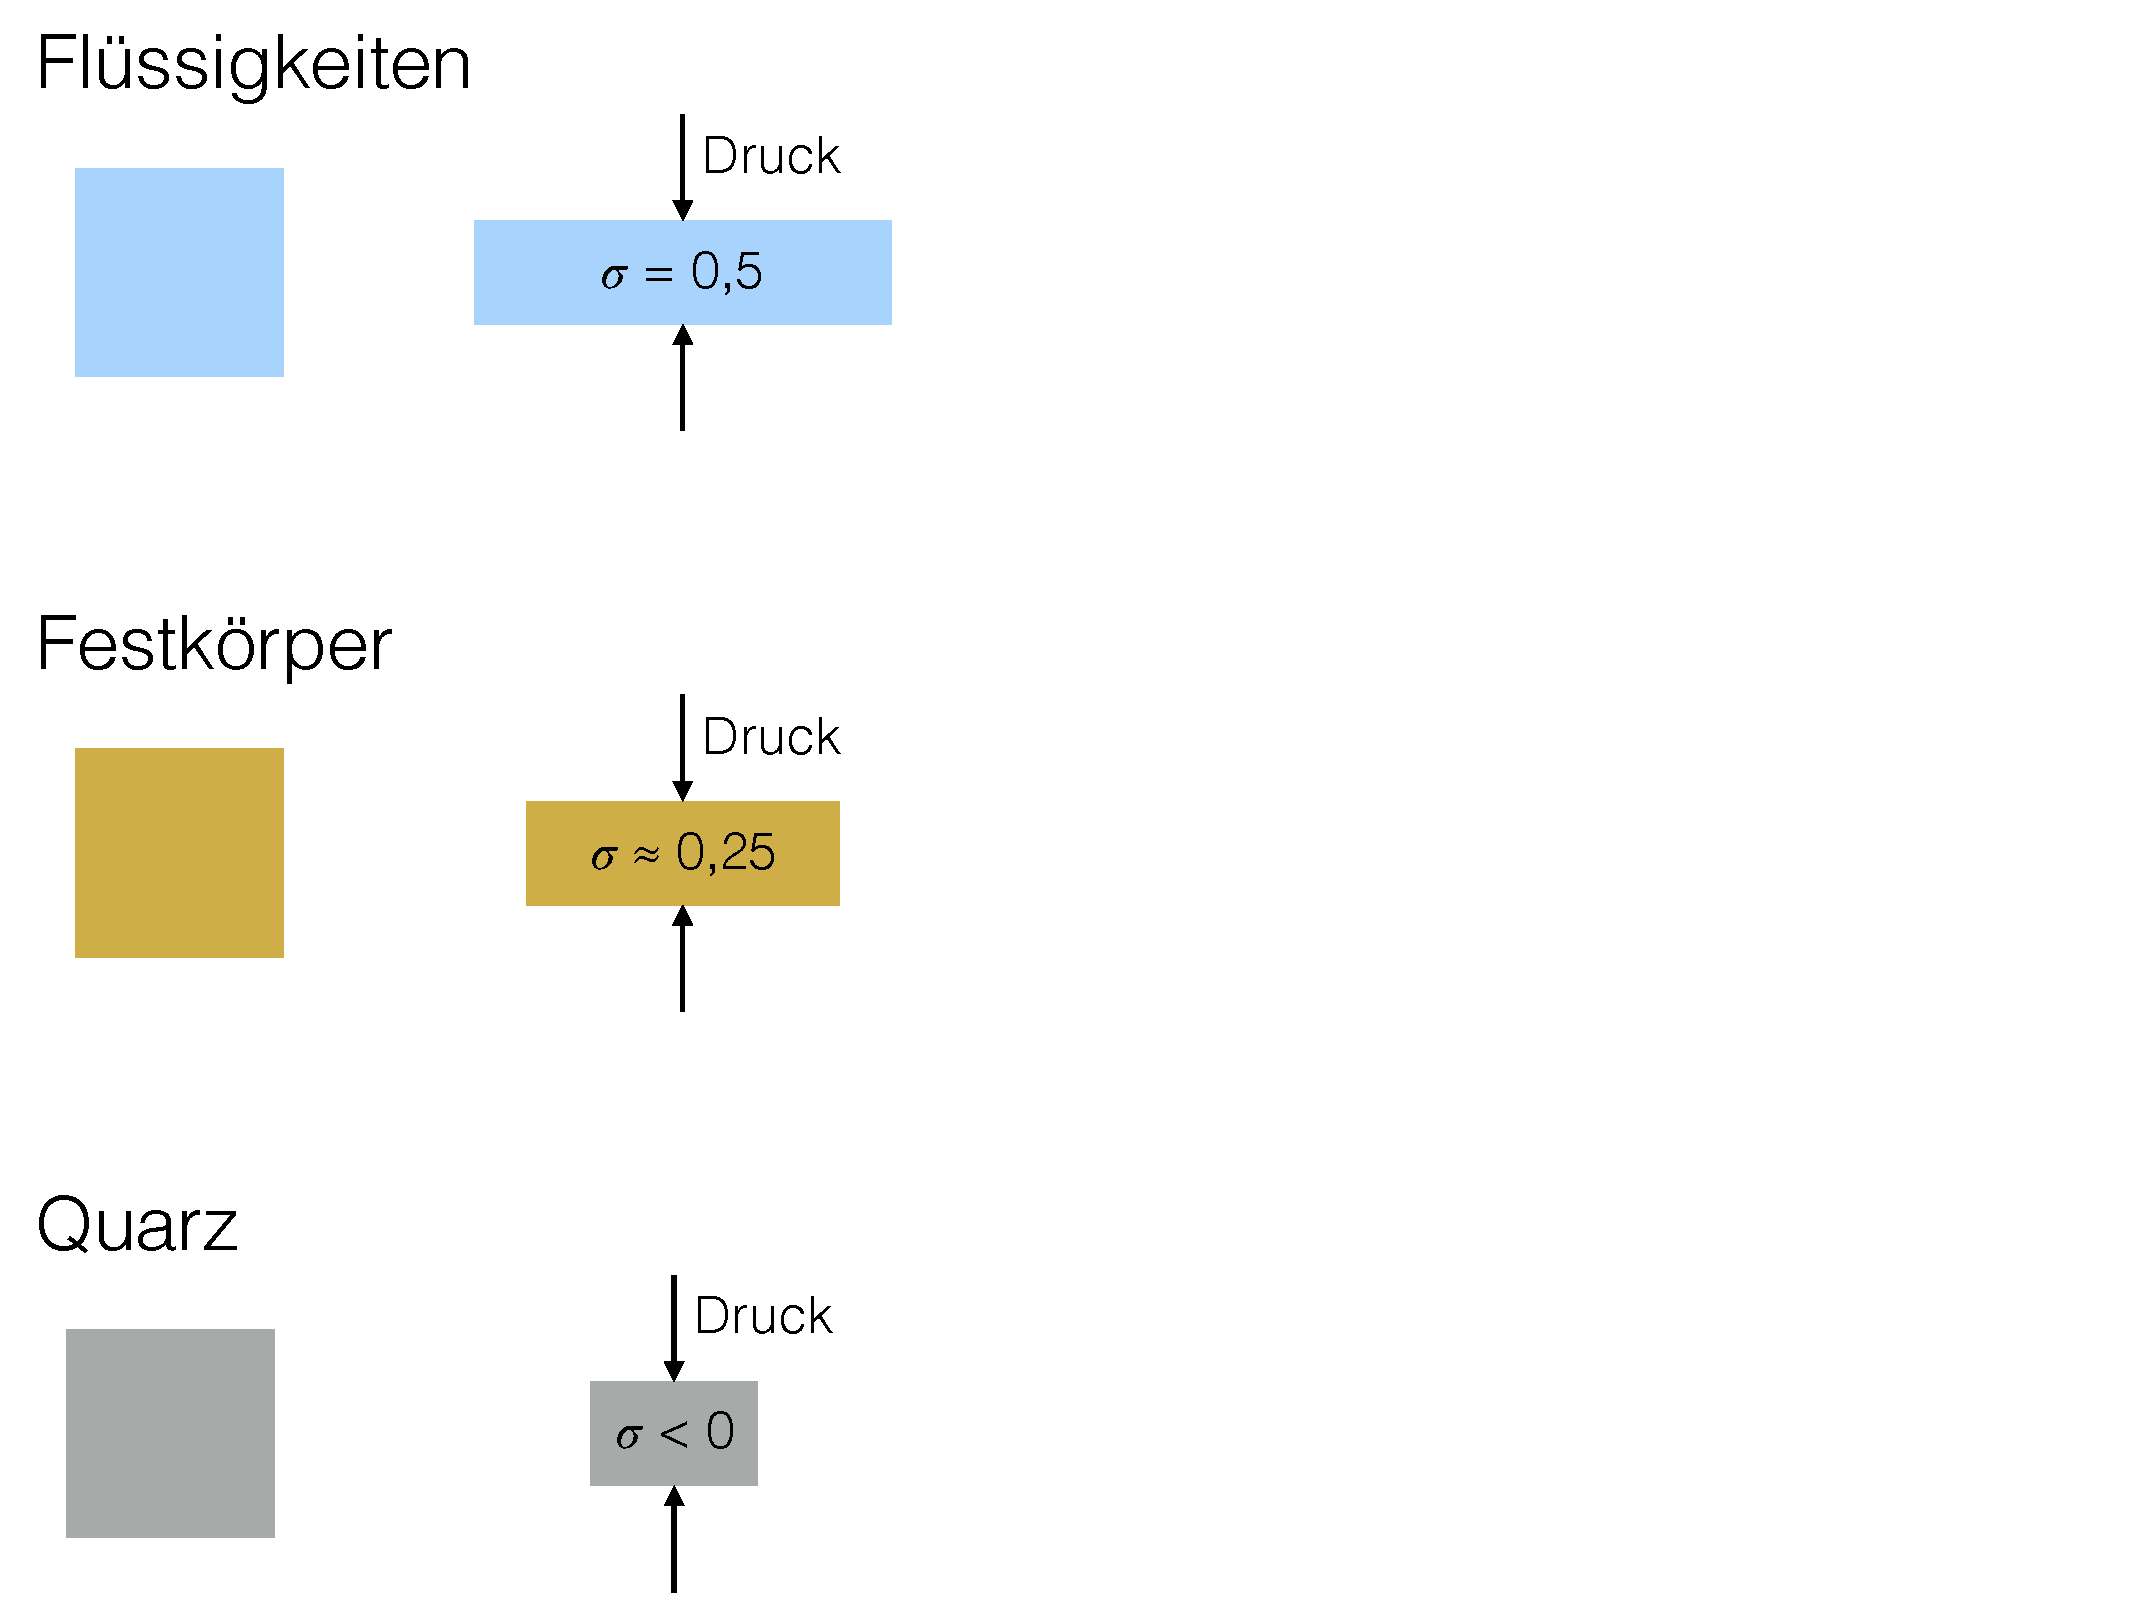
\includegraphics[scale = 0.3]{SeismikBilder/PoissonZahl}
\end{figure}


Die Poisson-Zahl berechnet sich zu: 
\begin{equation*}
	\sigma = \frac{\left( \frac{v_{\text{p}}}{v_{\text{s}}} \right)^2 - 2}{2 \cdot \left( \frac{v_{\text{p}}}{v_{\text{s}}} \right)^2 - 2} \qquad \text{mit } -1 < \sigma \leq 0,5 
\end{equation*}



\section{Wellenausbreitung}
Eine Welle wird an einer Schichtgrenze reflektiert, refraktiert und transmittiert.\begin{description}
	\item[Reflexion:] Ein Teil der Welle wird an der Schichtgrenze ins obere Medium zurückgeworfen.
	\item[Transmission:] Ein Teil der Welle wird uns untere Medium gebrochen. 
	\item[Refraktion:] Ein Teil der Welle läuft entlang der Schichtgrenze.
\end{description}


Bevor wir genauer auf die einzelnen Begriffe eingehen, schauen wir uns einmal die zu Grunde liegende physikalische Überlegung an.


\subsection{Huygen'sches Prinzip}
Jeder Punkt einer Wellenfront ist der Ausgangspunkt einer neuen Elementarwelle (Kreis- bzw. Kugelwelle). Diese neuen Wellen breiten sich mit der gleichen Geschwindigkeit aus wie die ursprüngliche Welle. Die neue Wellenfront ist dann die Einhüllende der einzelnen Elementarwellen.

\begin{figure}[H]
	\centering
	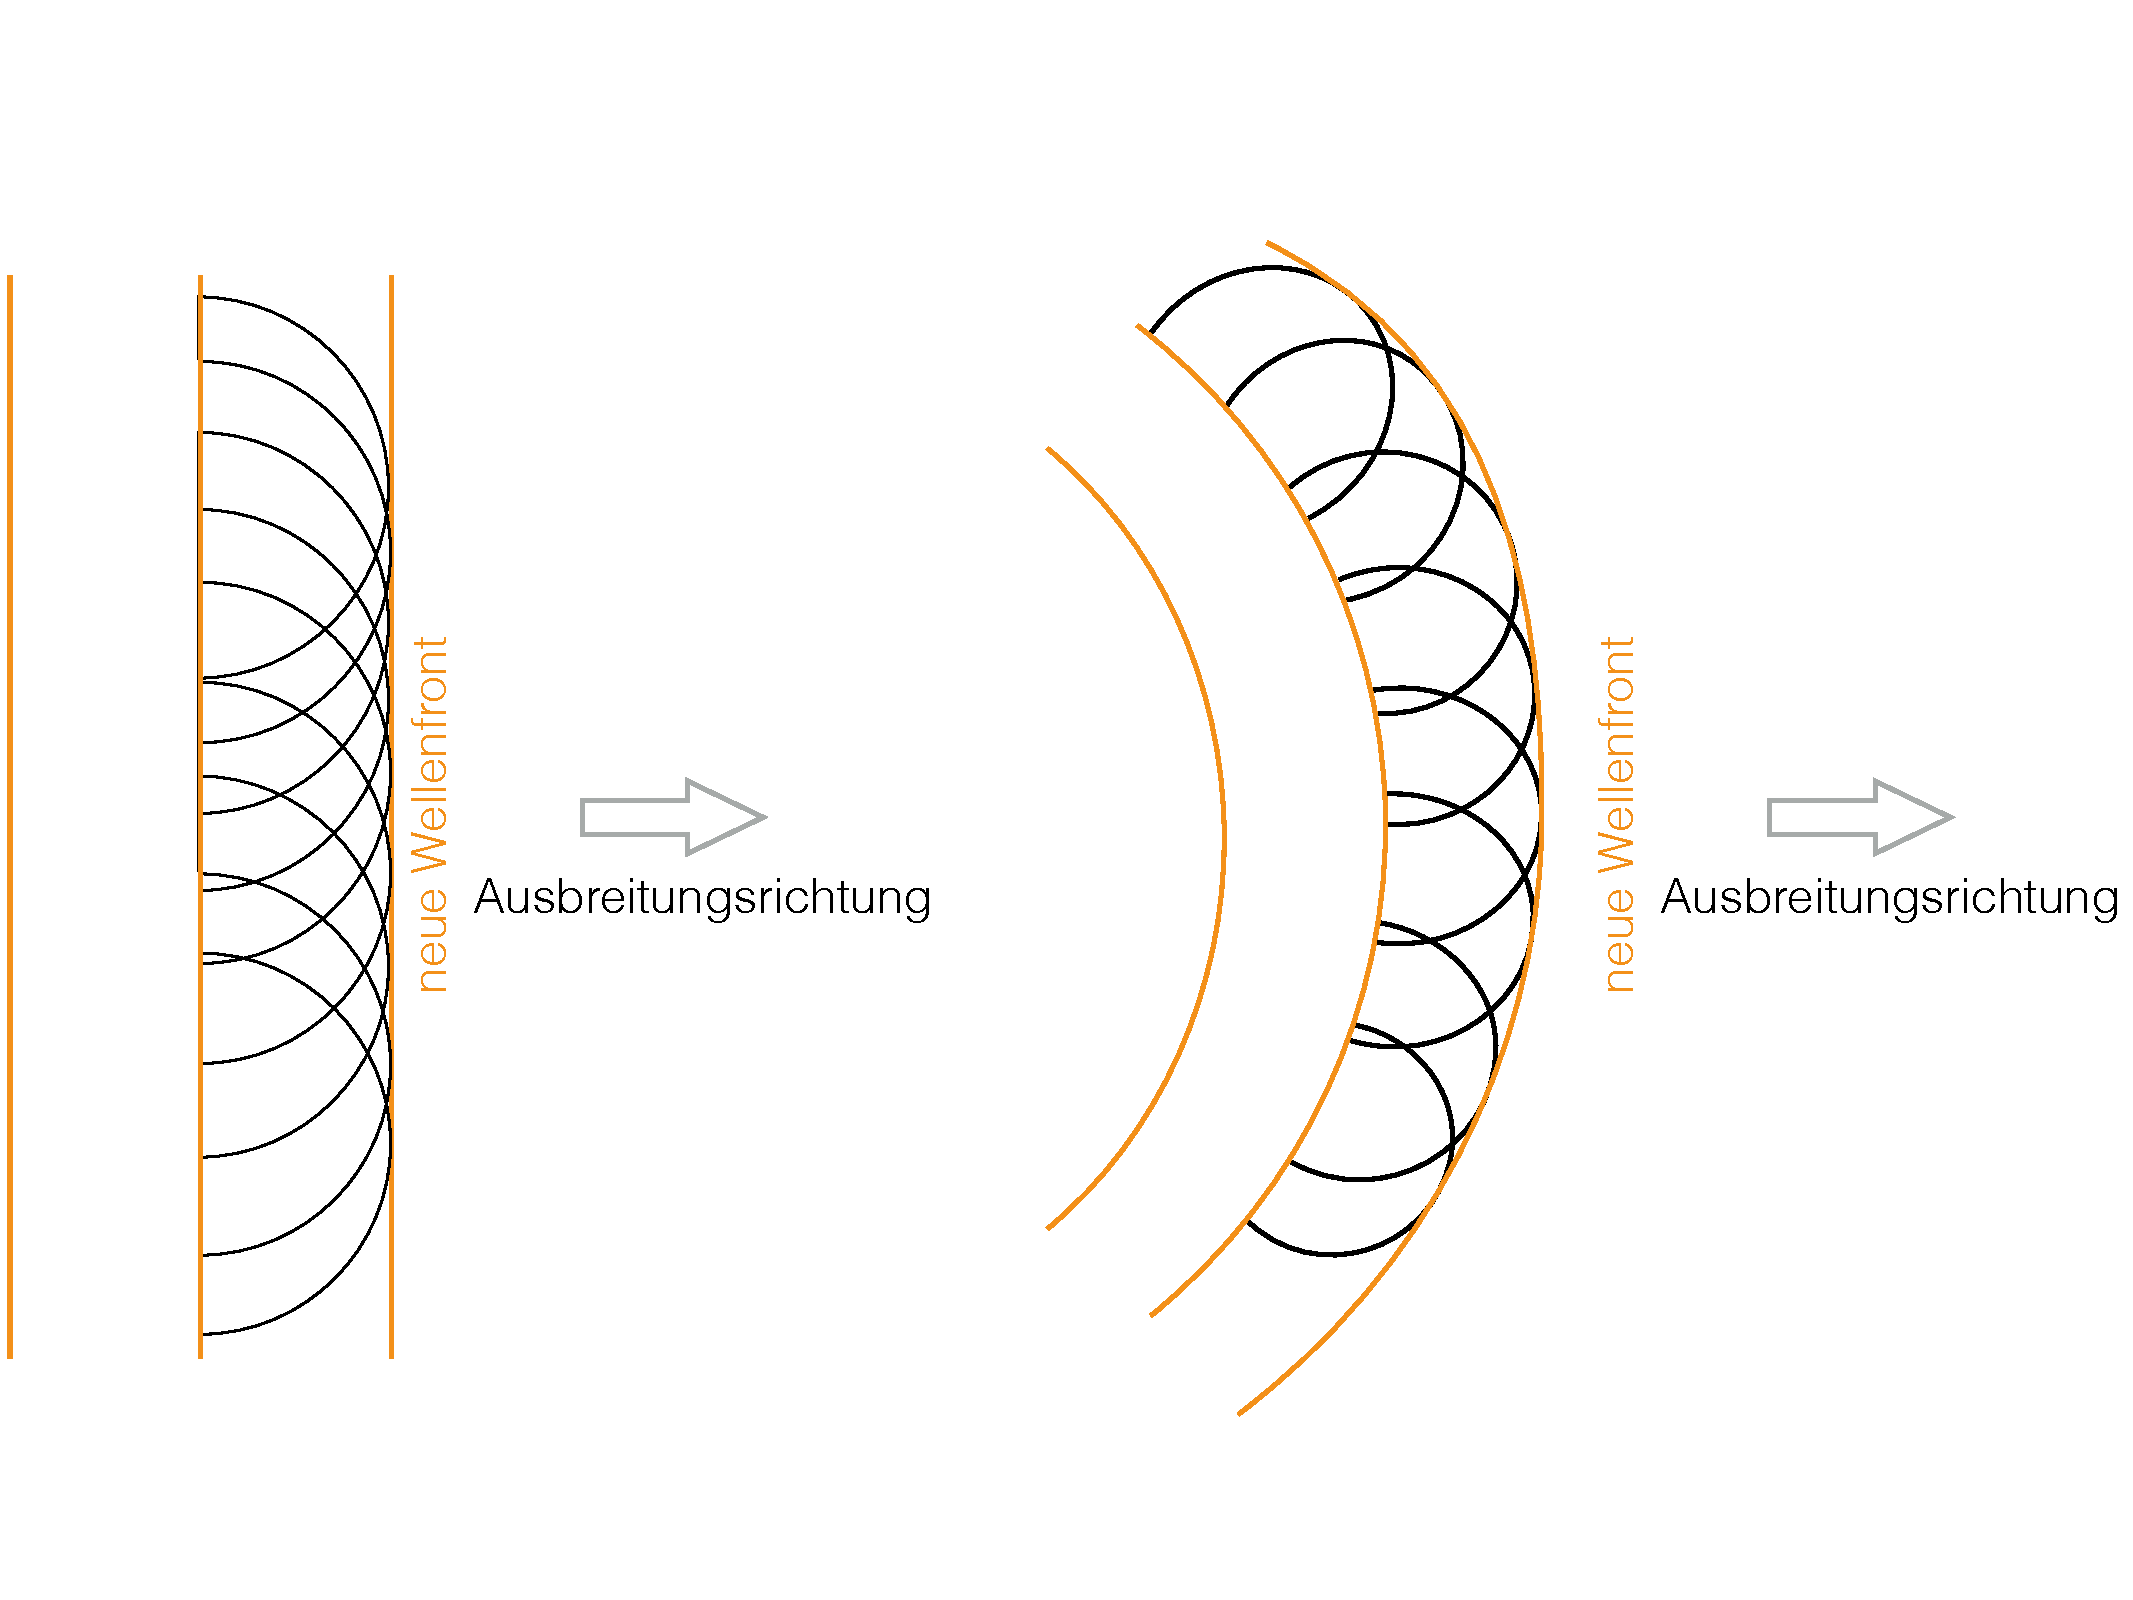
\includegraphics[width = \textwidth]{SeismikBilder/HuygensPrinzip1}
\end{figure}

Diese Grafik zeigt das Huygen'sche Prinzip für den Fall, dass die Welle ungehindert fortlaufen kann. Was aber passiert im Falle einer Reflexion oder Brechung an einer Schichtgrenze? 
Die zwei Grafiken unten zeigen, dass sich das Huygen'sche Prinzip einfach übertragen lässt. 

\begin{figure}[H]
	\centering
	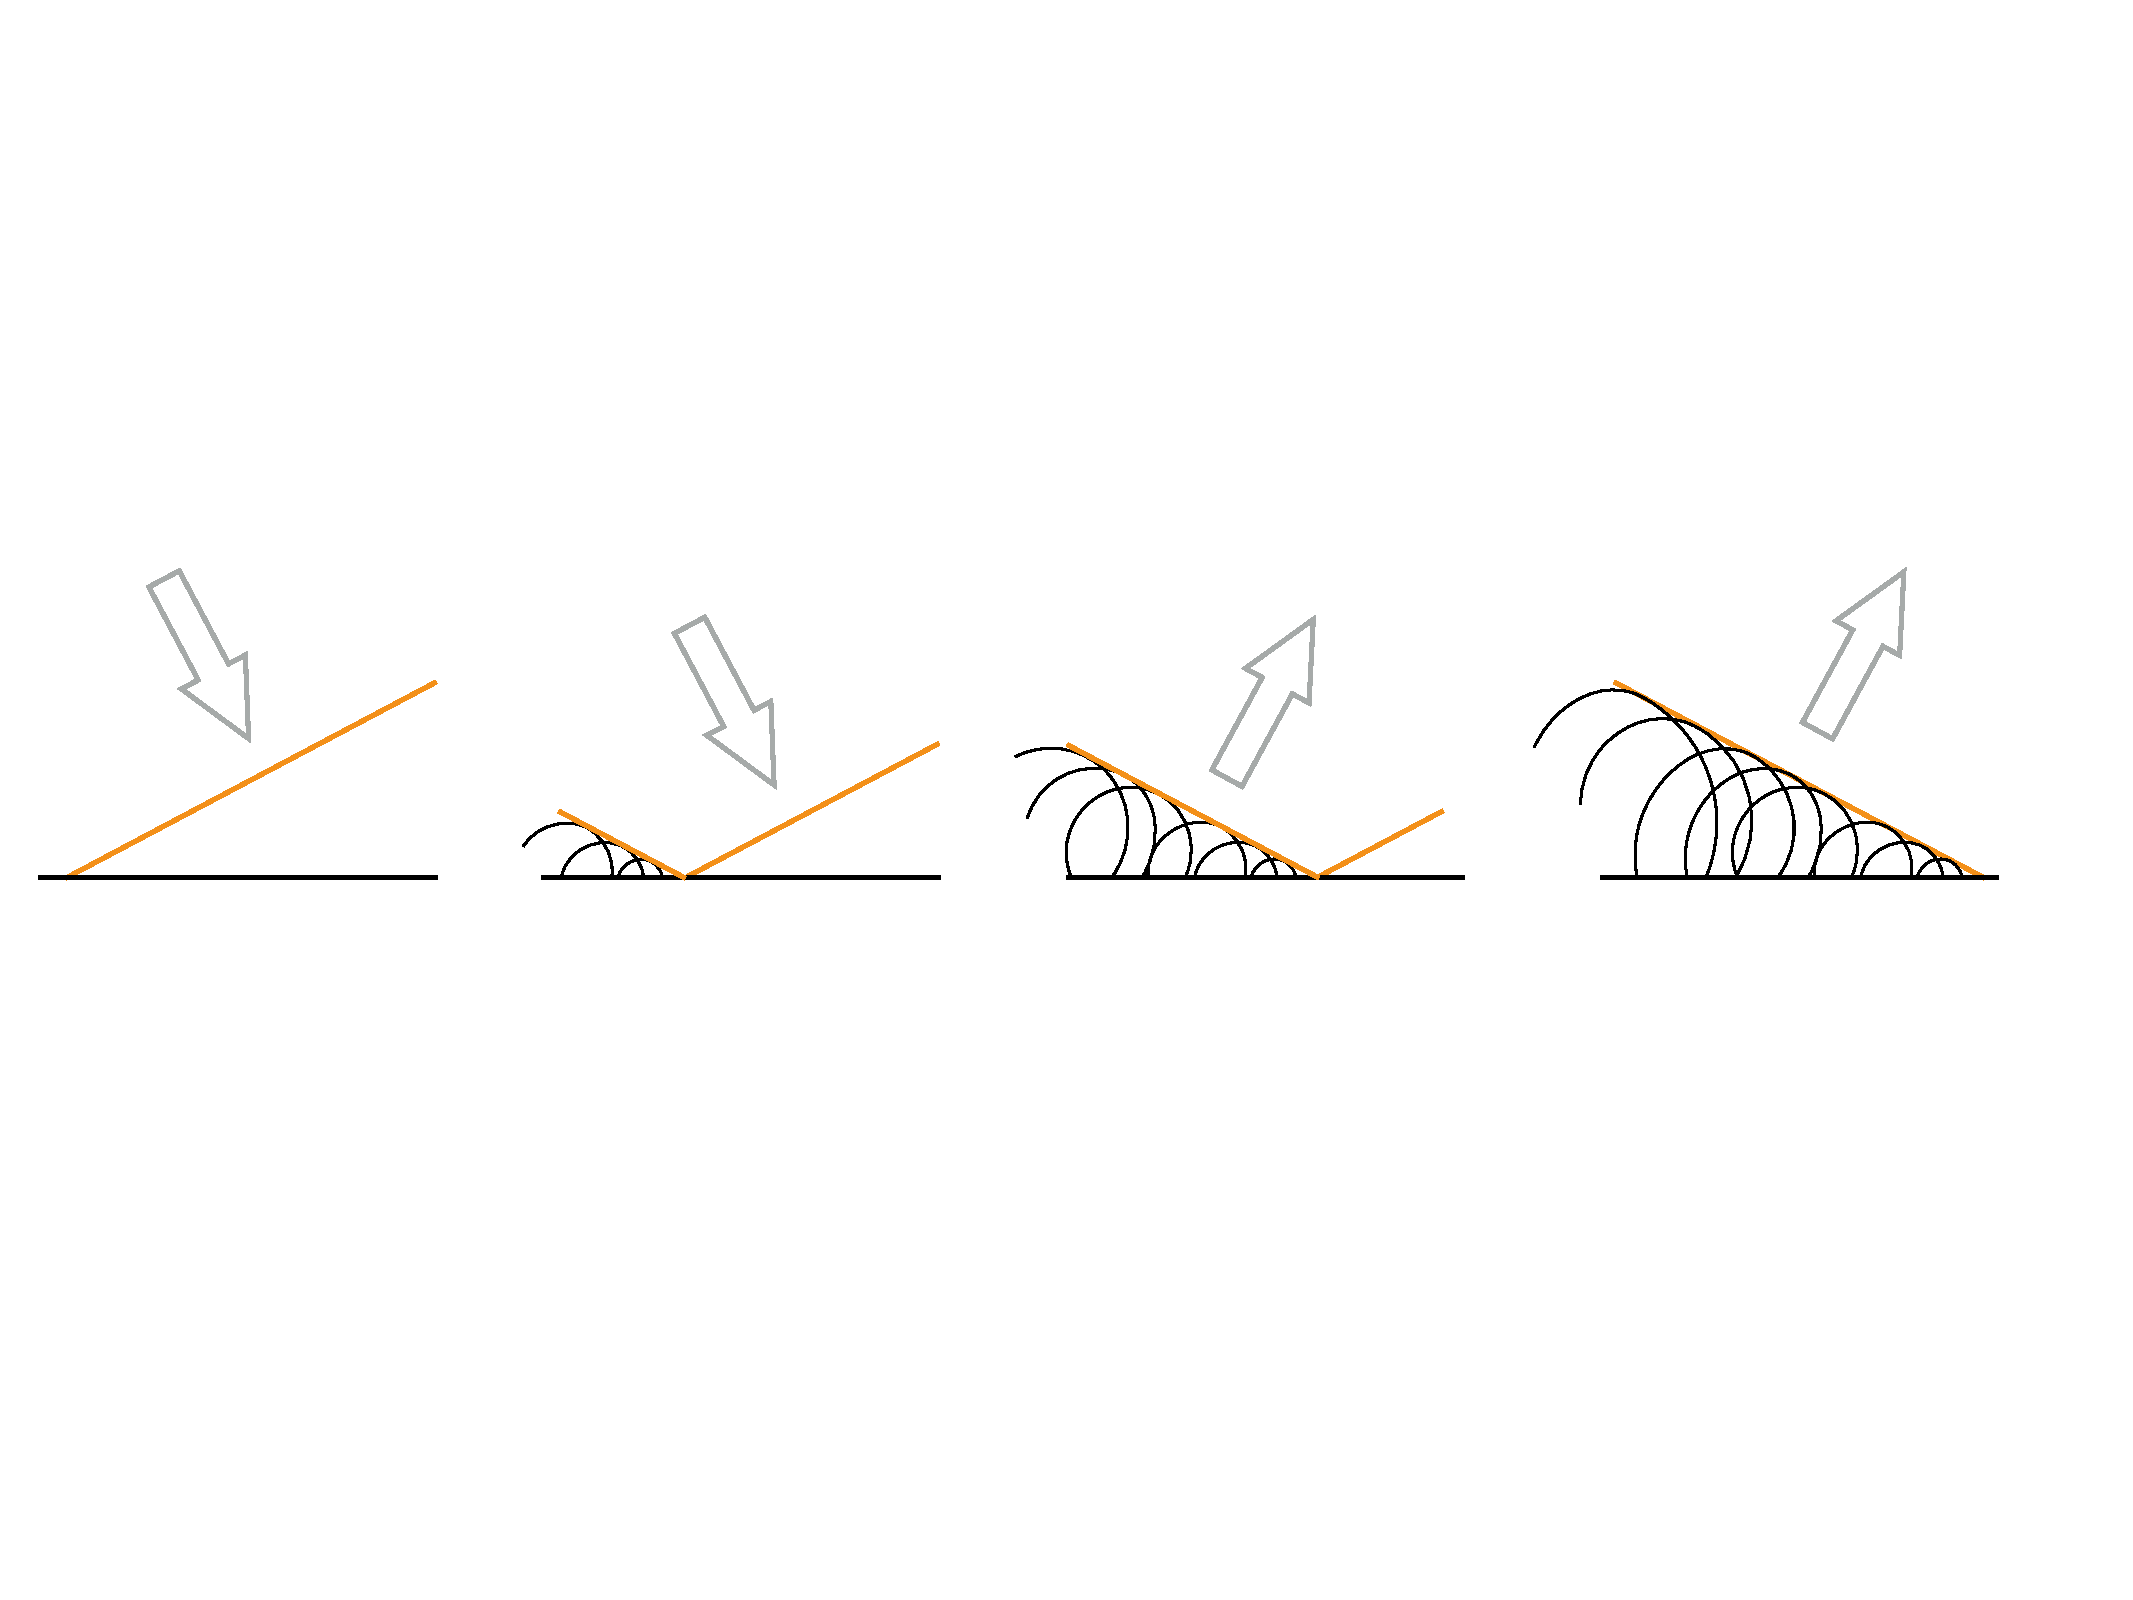
\includegraphics[width = \textwidth]{SeismikBilder/HuygensReflexion}
	\caption*{Reflexion}
\end{figure}

\begin{figure}[H]
	\centering
	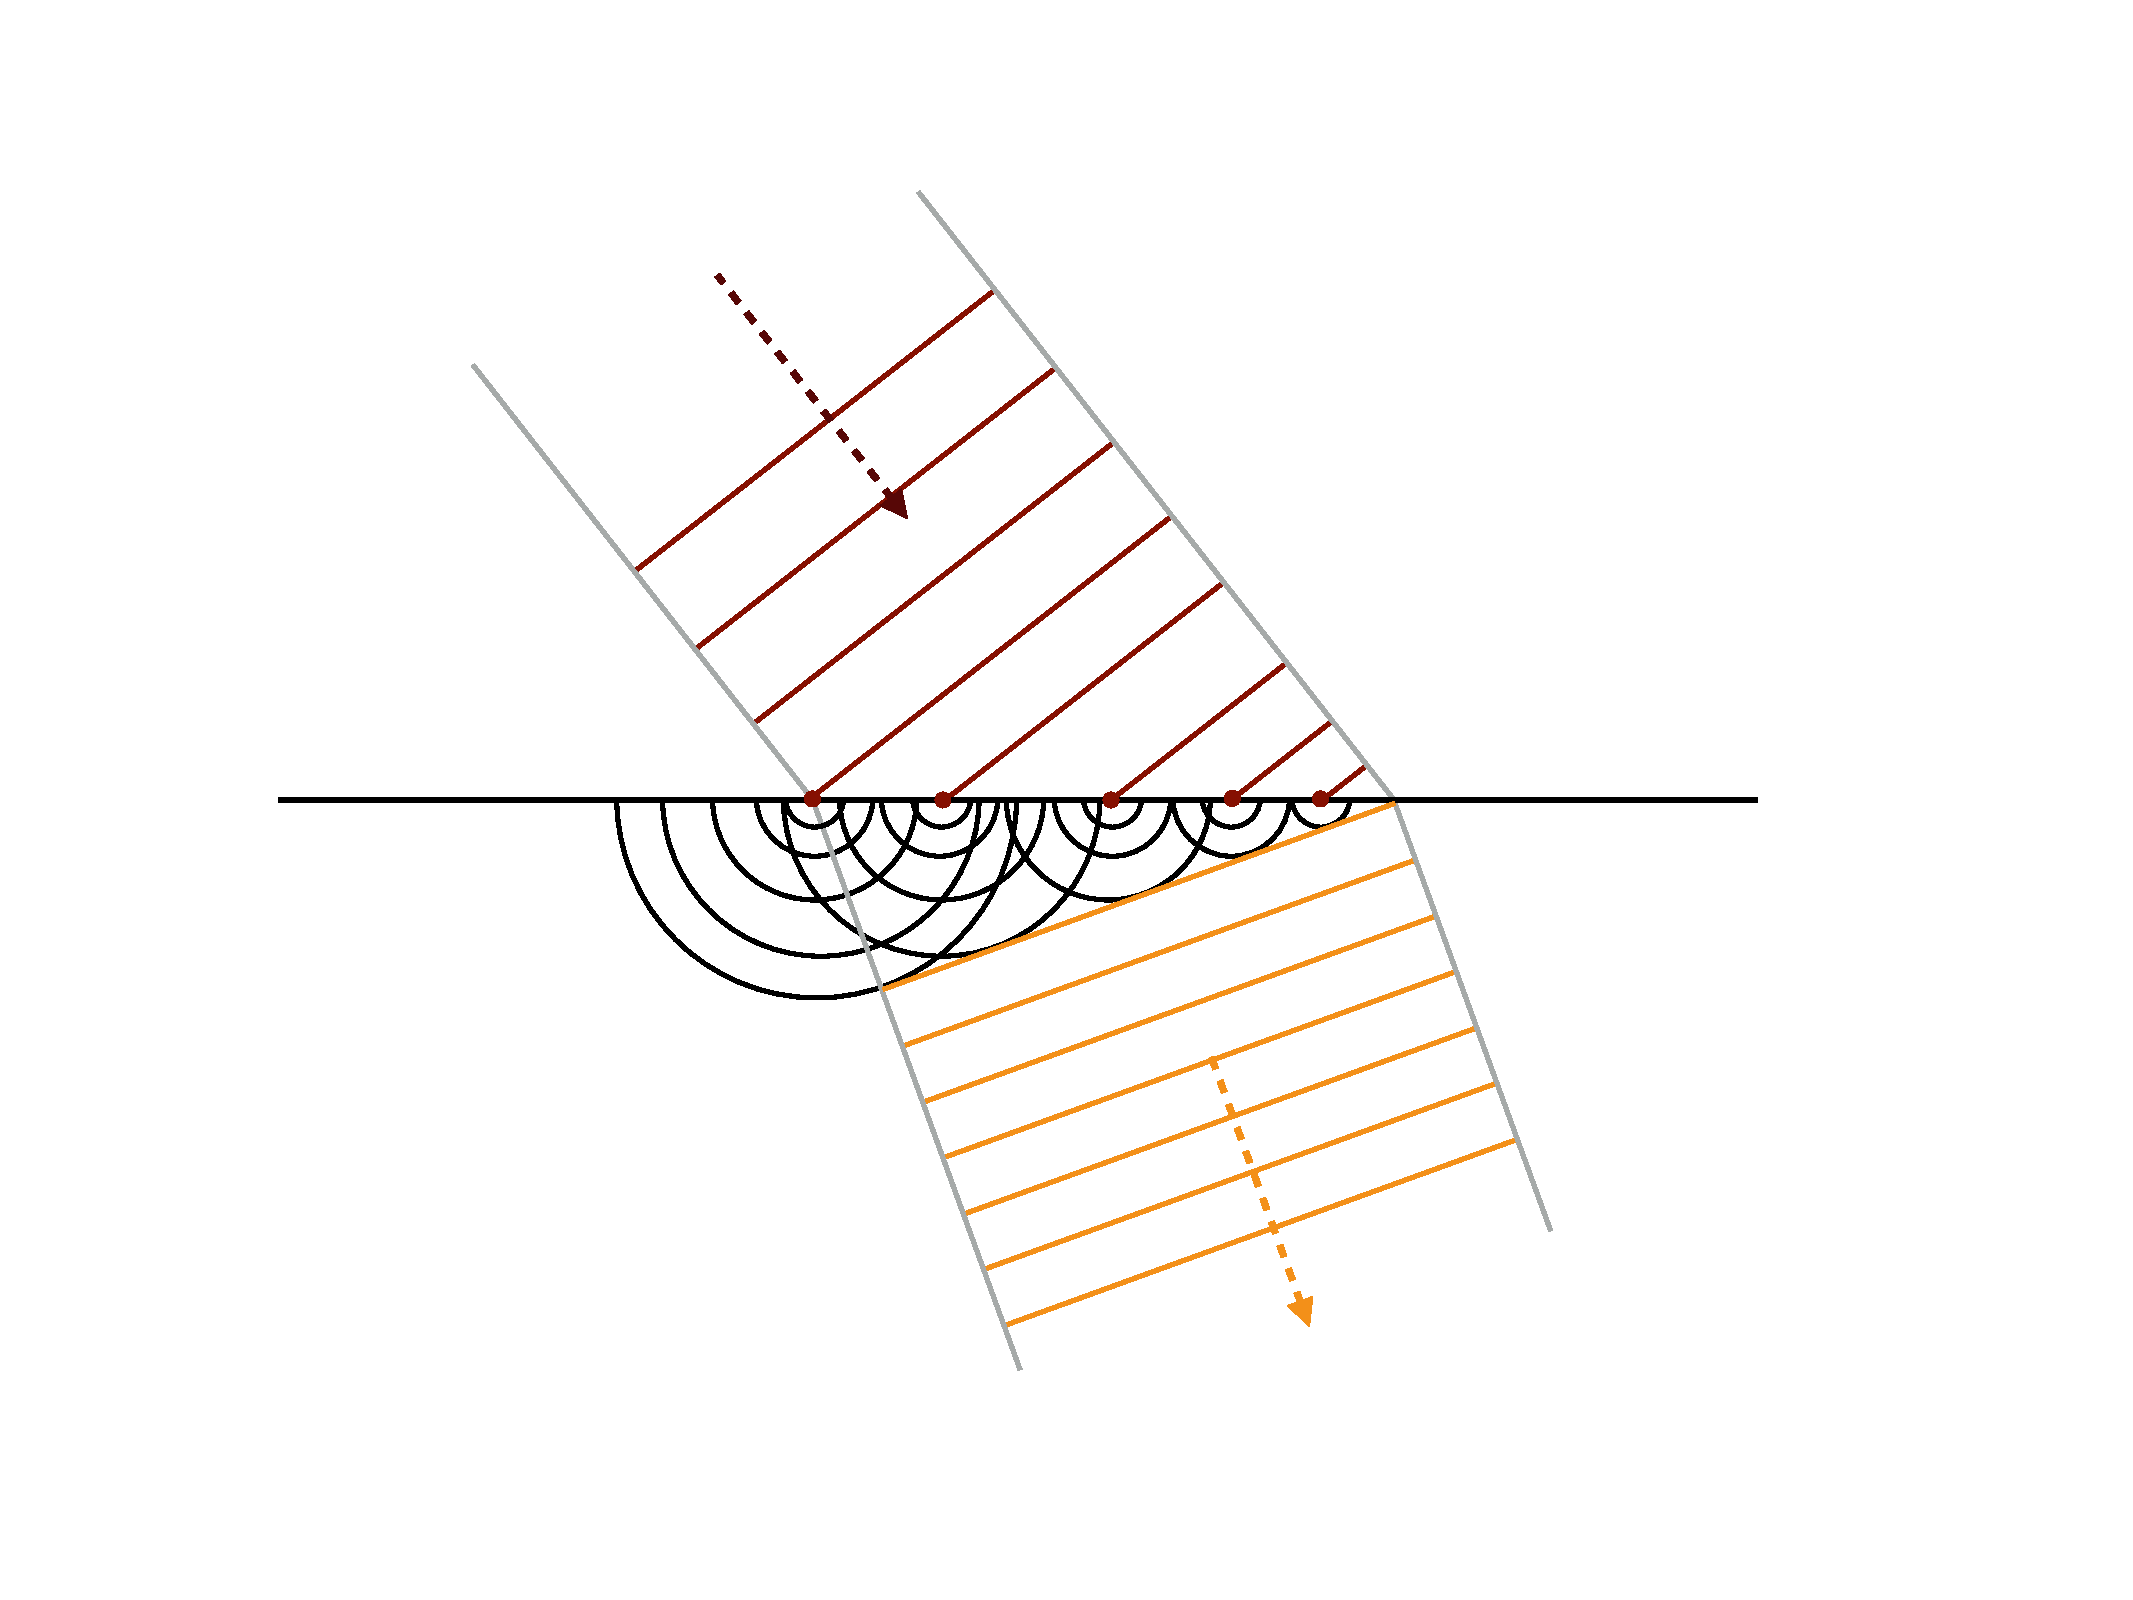
\includegraphics[width = \textwidth]{SeismikBilder/HuygensBrechung}
	\caption*{Brechung}
\end{figure}


\section{Brechungsgesetze}
Trifft eine Welle auf eine Schichtgrenze im Untergrund, wird sie gebrochen. Die Winkel, mit dem die Welle auftrifft, bzw. abgelenkt wird lässt sich einfach berechnen mit Hilfe des \textbf{Snellius'schen Brechungsgesetz}:

\begin{figure}[H]
	\begin{subfigure}[m]{0.5\textwidth}
	\centering
		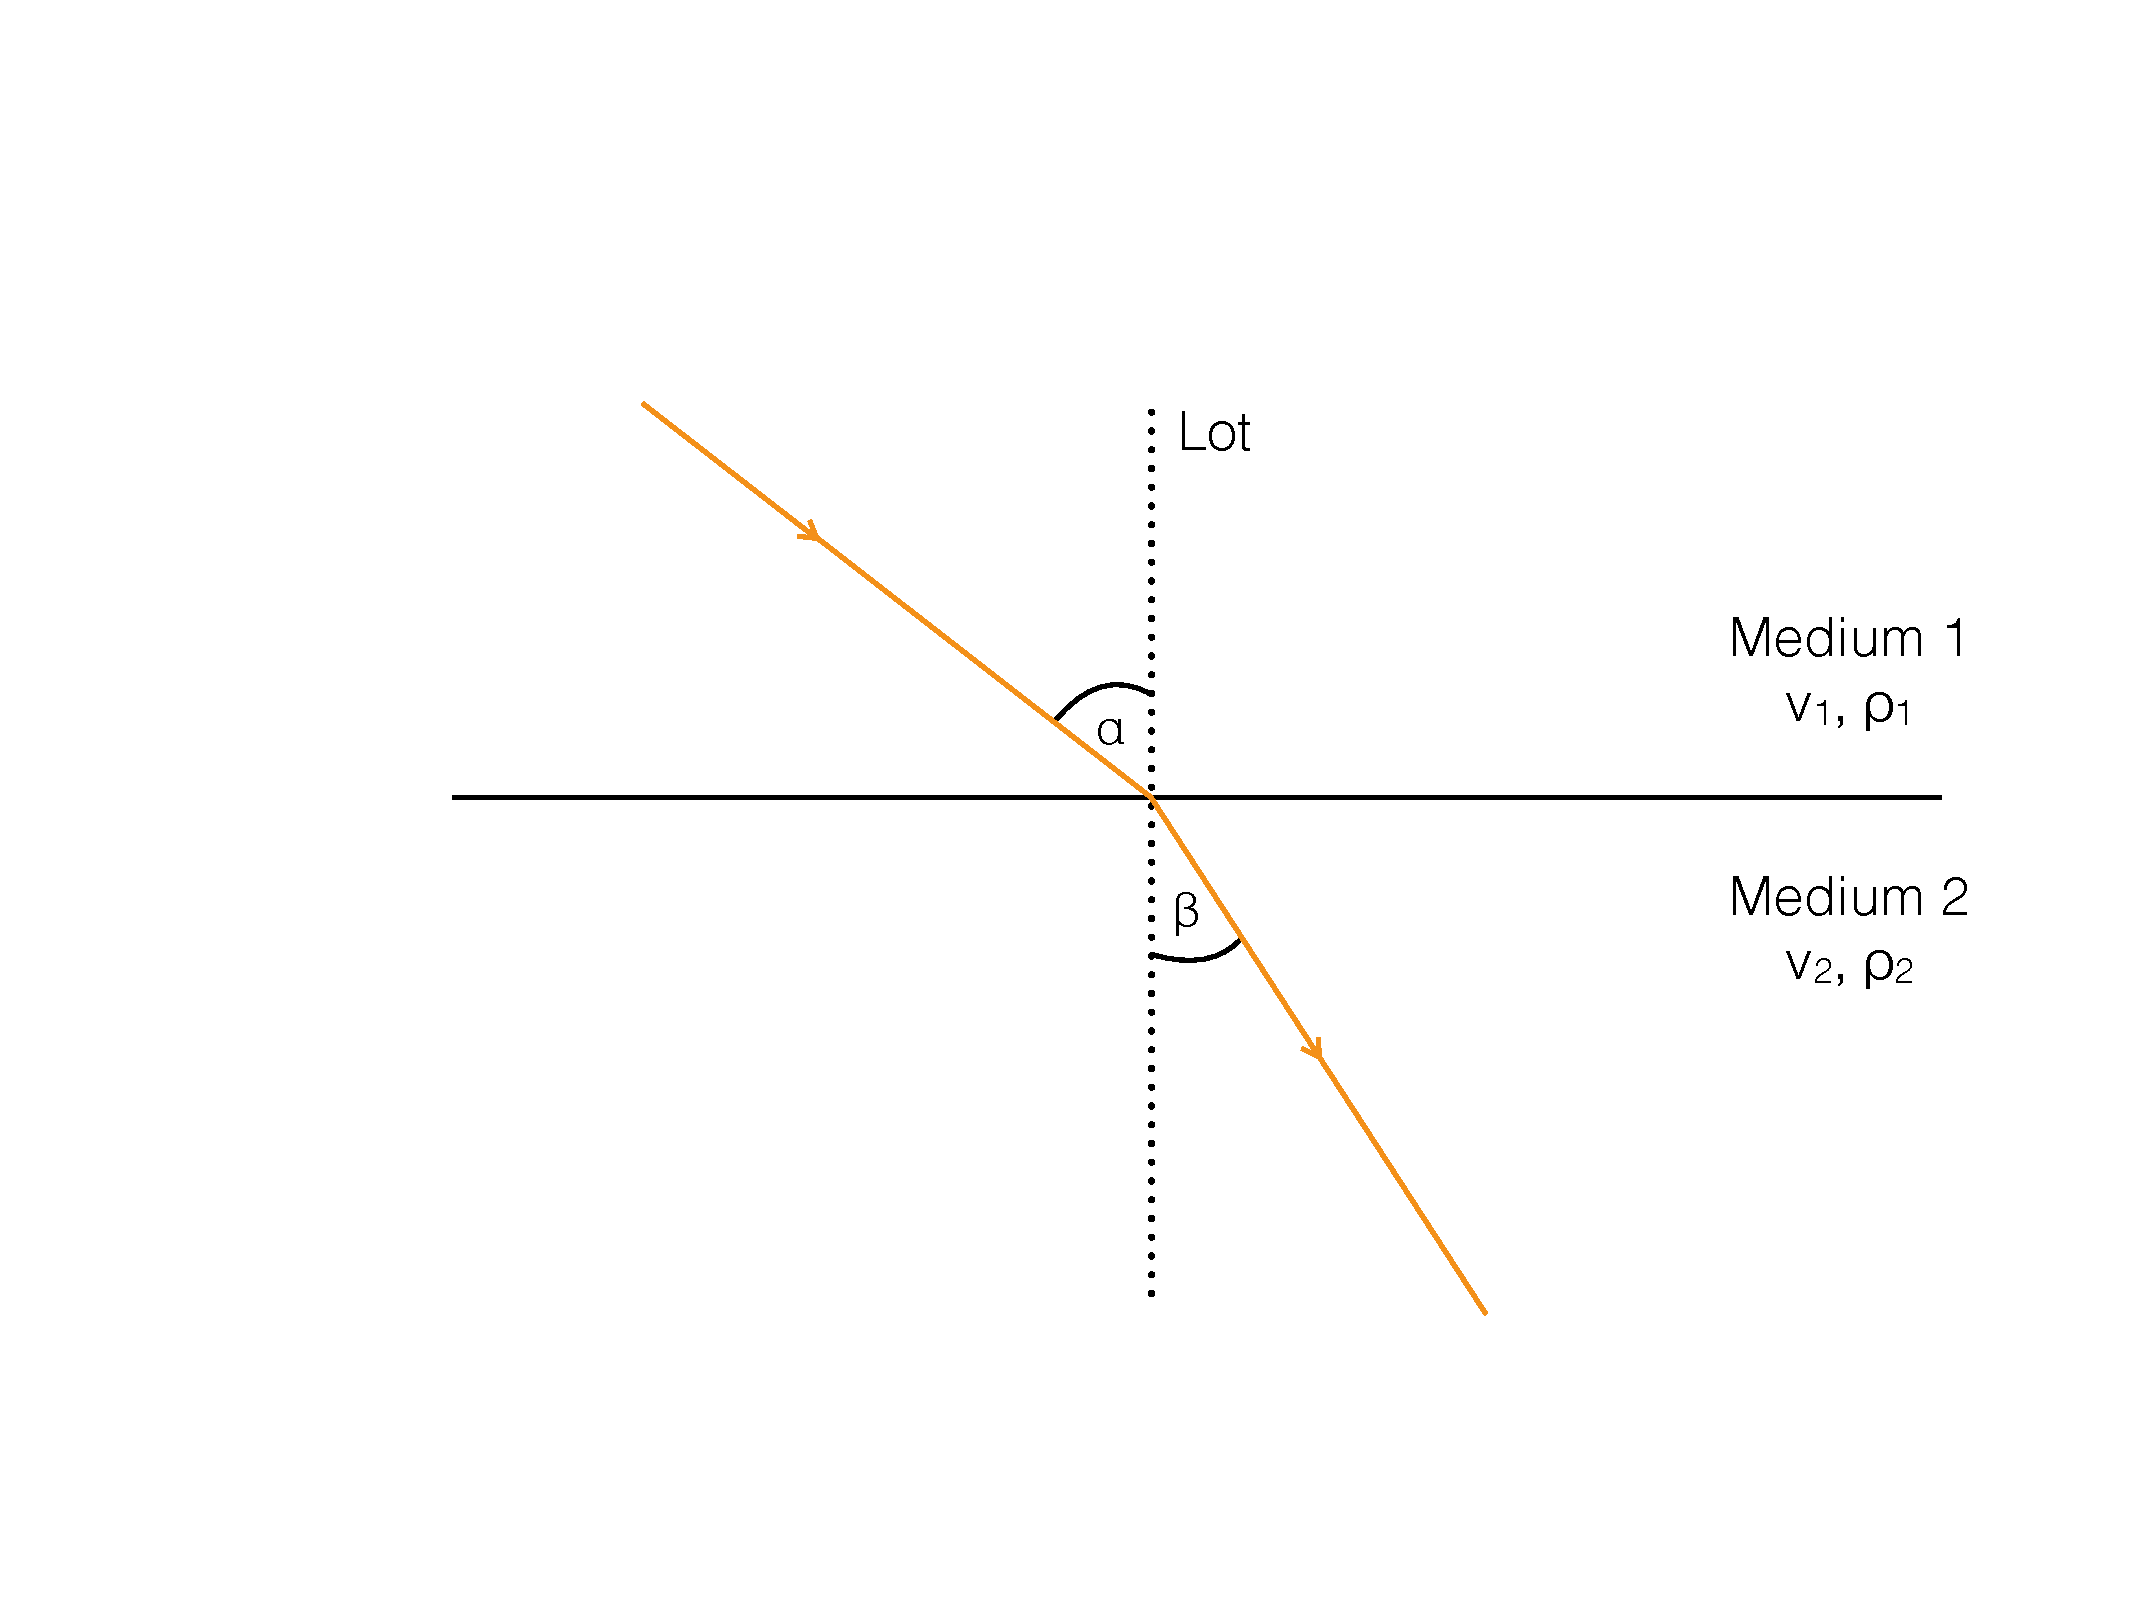
\includegraphics[scale=0.3]{SeismikBilder/Brechungsgesetz}
	\end{subfigure}
	\begin{subfigure}[m]{0.75\textwidth}
	\centering
		\[\begin{aligned}
			\frac{sin(\alpha)}{sin(\beta)} = \frac{v_1}{v_2}
		\end{aligned}\]
	\end{subfigure}
\end{figure}


Wir schauen uns noch die Herleitung dieses Gesetzes an. Als Hilfsmittel nehmen wir uns die Grafik von oben, die wir um einige Größen erweitern. 

\begin{figure}[H]
	\centering
	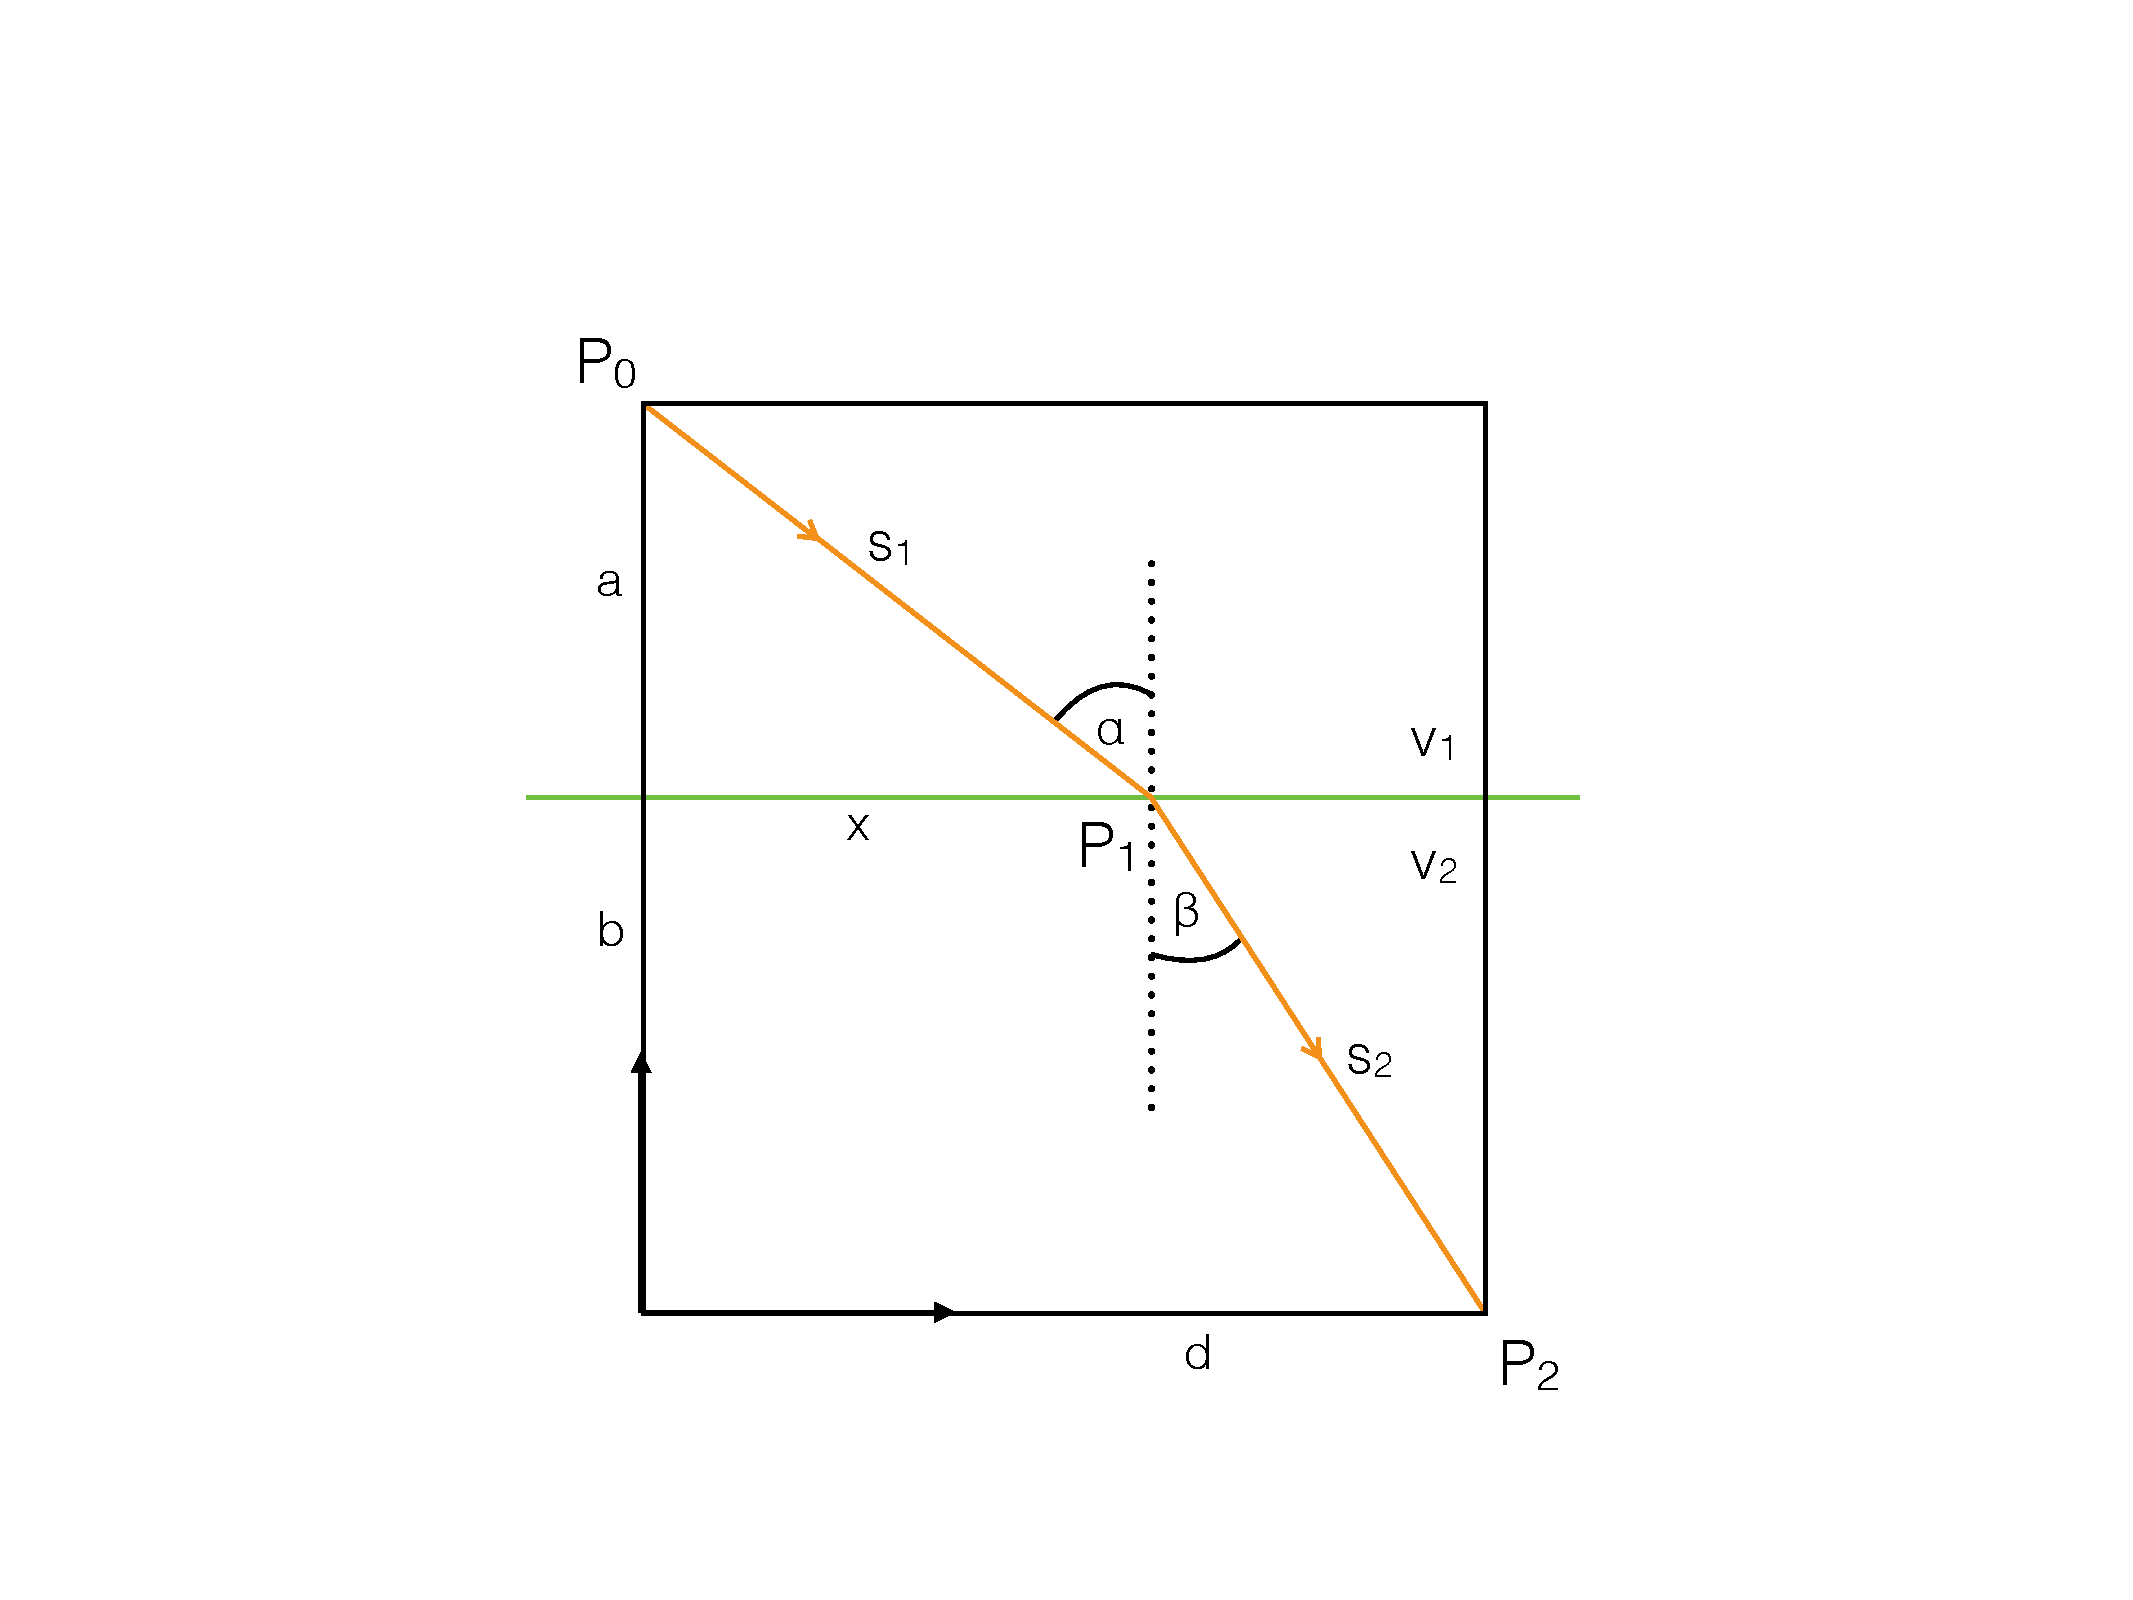
\includegraphics[scale = 0.5]{SeismikBilder/GrafikHerleitung}
\end{figure}
 
Eine Welle will immer den schnellsten Weg nehmen, also den Weg mit kürzester Laufzeit (\textbf{Fermat'sches Prinzip}).

Die Welle beginnt in unserem Beispiel bei $P_0 = \left( 0, \ a + b \right)$ und geht durch den Punkt $P_1 = \left( x, \ b \right)$ zu $P_2 = \left( d, \ 0 \right)$.

Im oberen Medium hat die Welle die konstante Geschwindigkeit $v_1$ und im Unteren $v_2$. Die Welle erfährt keine Beschleunigung. Aus diesem Grund können wir für die Berechnung der Laufzeit $t(x)$ der Welle den einfachen physikalischen Zusammenhang $s = v \cdot t$ verwenden. \begin{align*}
	t(x) = t_1 + t_2 = \frac{s_1}{v_1} + \frac{s_2}{v_2} = \frac{|P_1 - P_0|}{v_1} + \frac{|P_2 - P_1|}{v_2} = \frac{\sqrt{a^2 + x^2}}{v_1} + \frac{\sqrt{(d - x)^2 + b^2}}{v_2}
\end{align*}

Da wir die minimale Laufzeit suchen, leiten wir $t(x)$ ab und setzen diesen Term 0. \begin{align*}
	\frac{dt}{dx} = \frac{x}{  v_1 \cdot \sqrt{a^2 + x^2}} - \frac{(d - x)}{ v_2 \cdot \sqrt{(d - x)^2 + b^2}} \overset{!}{=} 0
\end{align*}

Wir betrachten erneut die Grafik und sehen: \begin{align*}
	x &= sin(\alpha) \cdot \sqrt{a^2 + x^2} \\
	d - x &= sin(\beta) \cdot \sqrt{(d - x)^2 + b^2}
\end{align*}

Daraus ergibt sich: \begin{equation*}
	0 = \frac{sin(\alpha)}{v_1} - \frac{sin(\beta)}{v_2}
\end{equation*} 
Und daraus wiederum das Brechungsgesetz \begin{equation*}
	\frac{sin(\alpha)}{sin(\beta)} = \frac{v_1}{v_2}
\end{equation*}

Mit dem Snellius'schen Brechungsgesetz lässt sich beispielsweise die bekannte Aussage "`Einfallswinkel = Ausfallswinkel"' leicht zeigen: 

\begin{figure}[H]
	\begin{subfigure}[m]{0.5\textwidth}
	\centering
		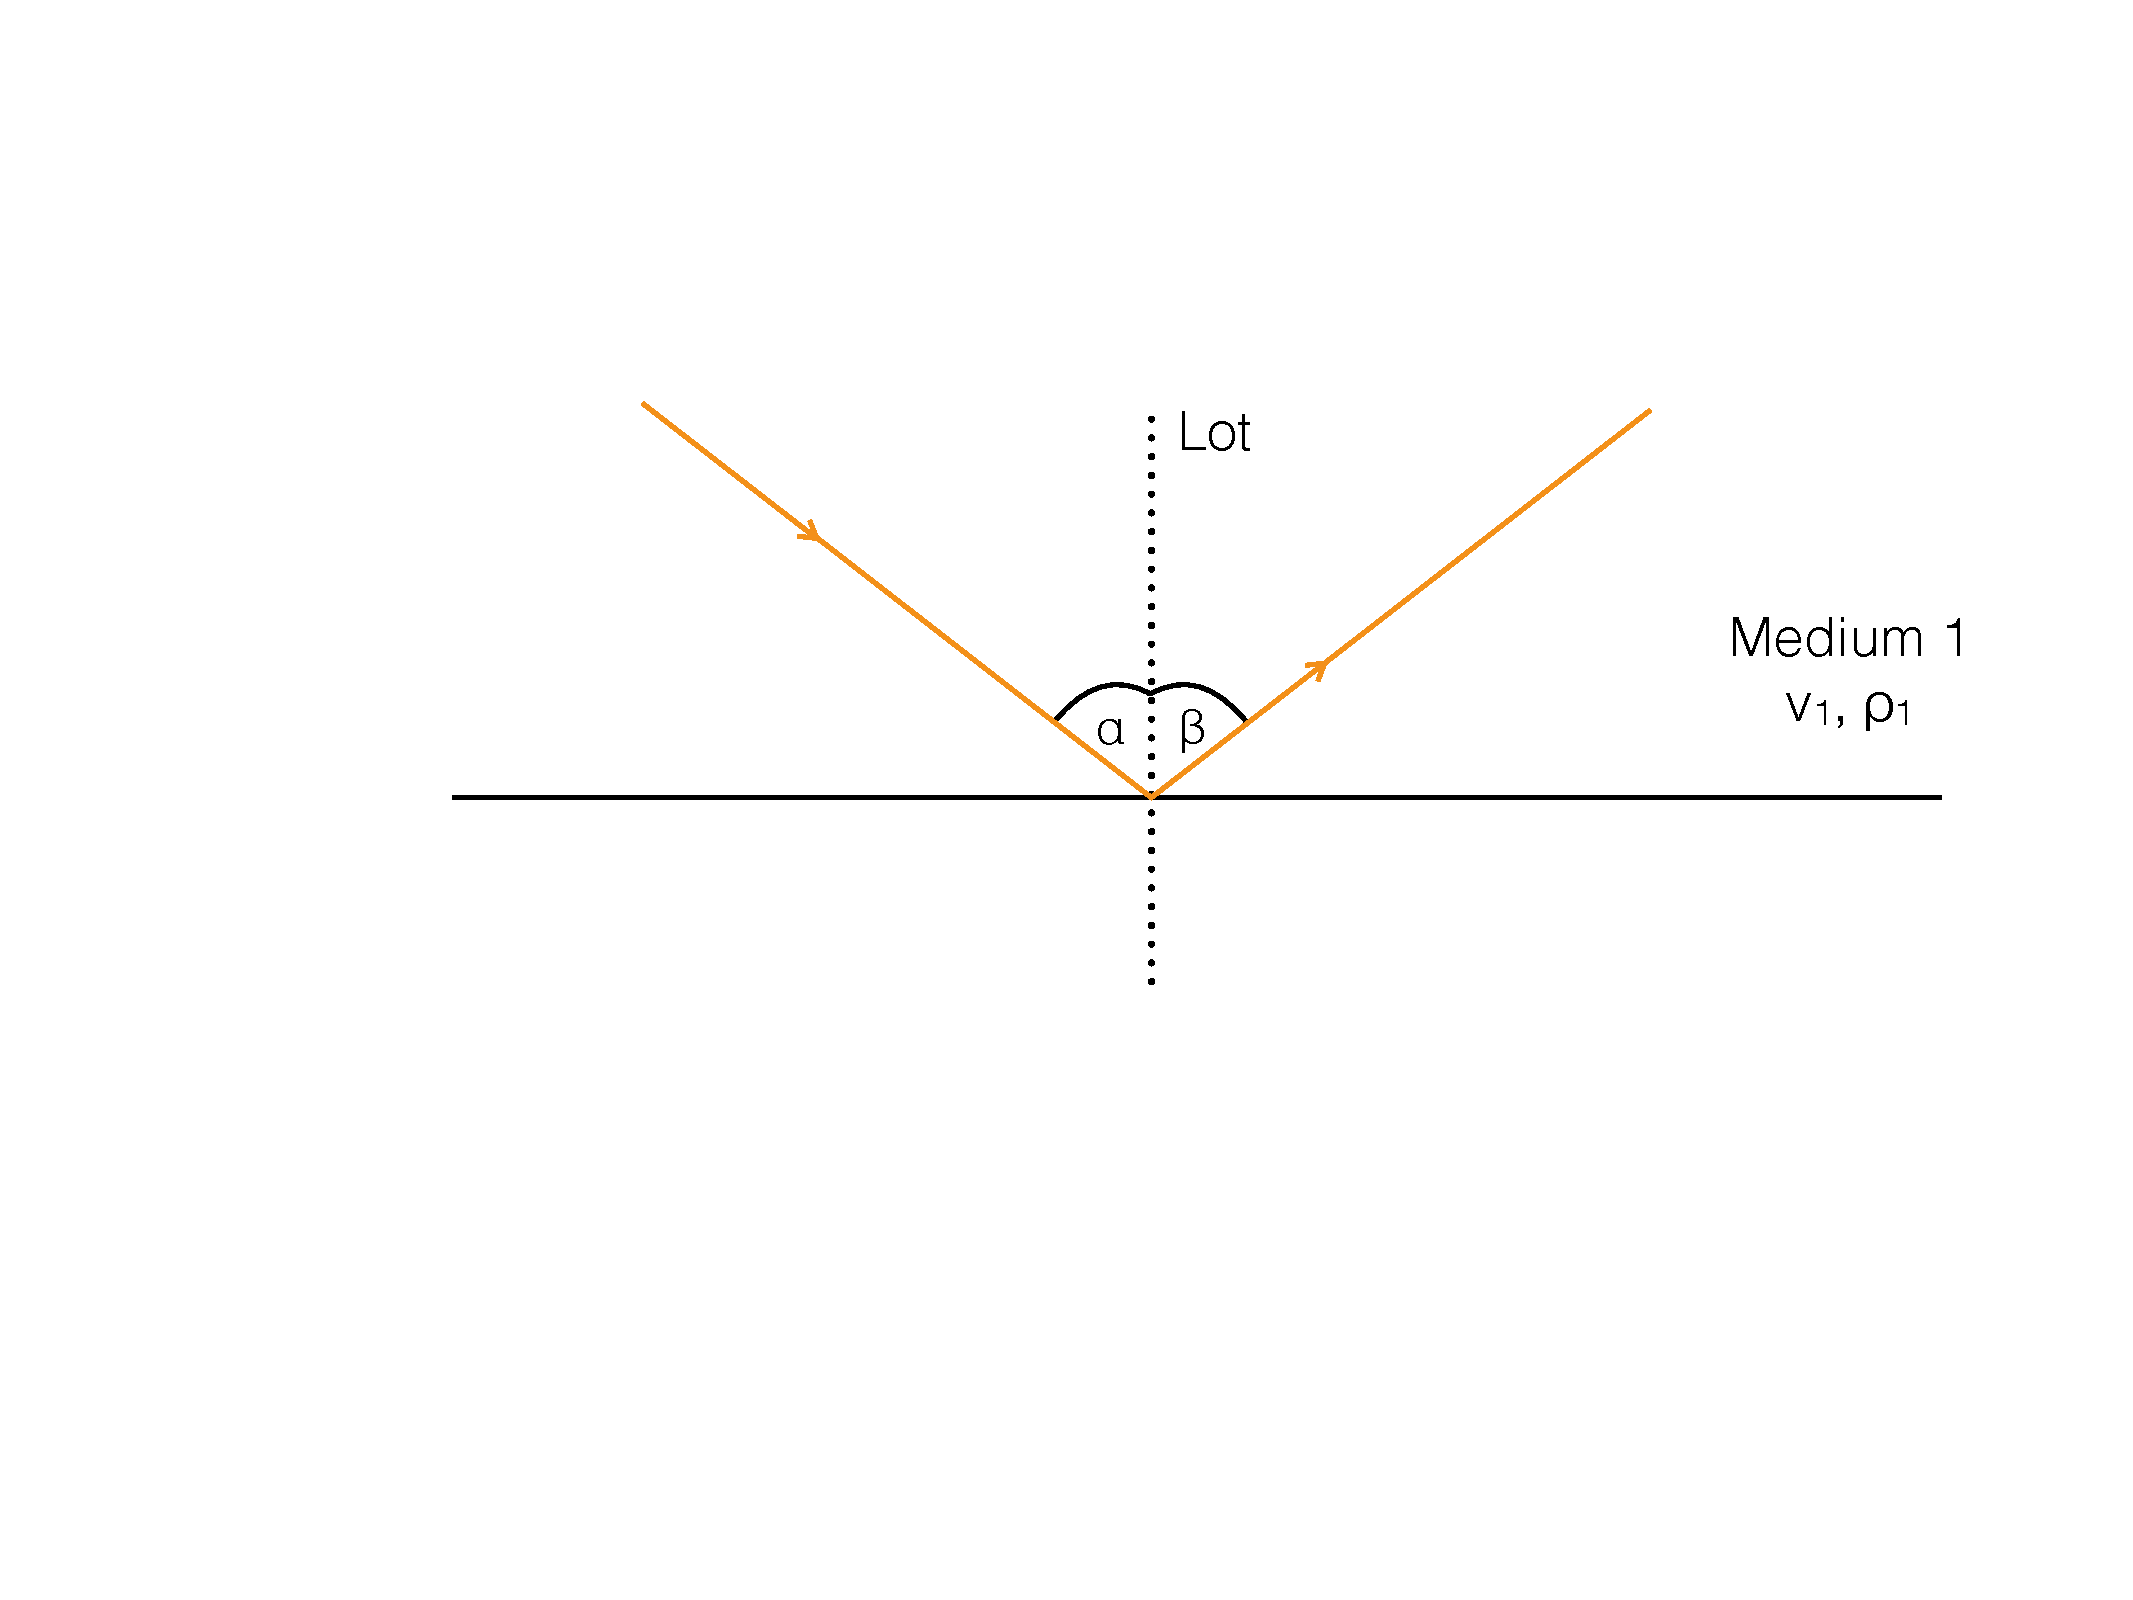
\includegraphics[scale=0.3]{SeismikBilder/EinfallsAusfallswinkel}
	\end{subfigure}
	\begin{subfigure}[m]{0.75\textwidth}
	\centering
		\[\begin{aligned}
			\frac{sin(\alpha)}{v_1} = \frac{sin(\beta)}{v_2} \\ \text{mit } v_1 = v_2 \quad \text{folgt } \alpha = \beta 
 		\end{aligned}\]
	\end{subfigure}
\end{figure}


\subsection{Reflexion und Transmission}
Die Streuwinkel der Welle nach Auftreffen auf die Grenzschicht für Reflexion und Transmission ergibt sich durch direkte Anwendung des Snellius'schen Brechungsgesetzes.

\begin{figure}[H]
	\centering
	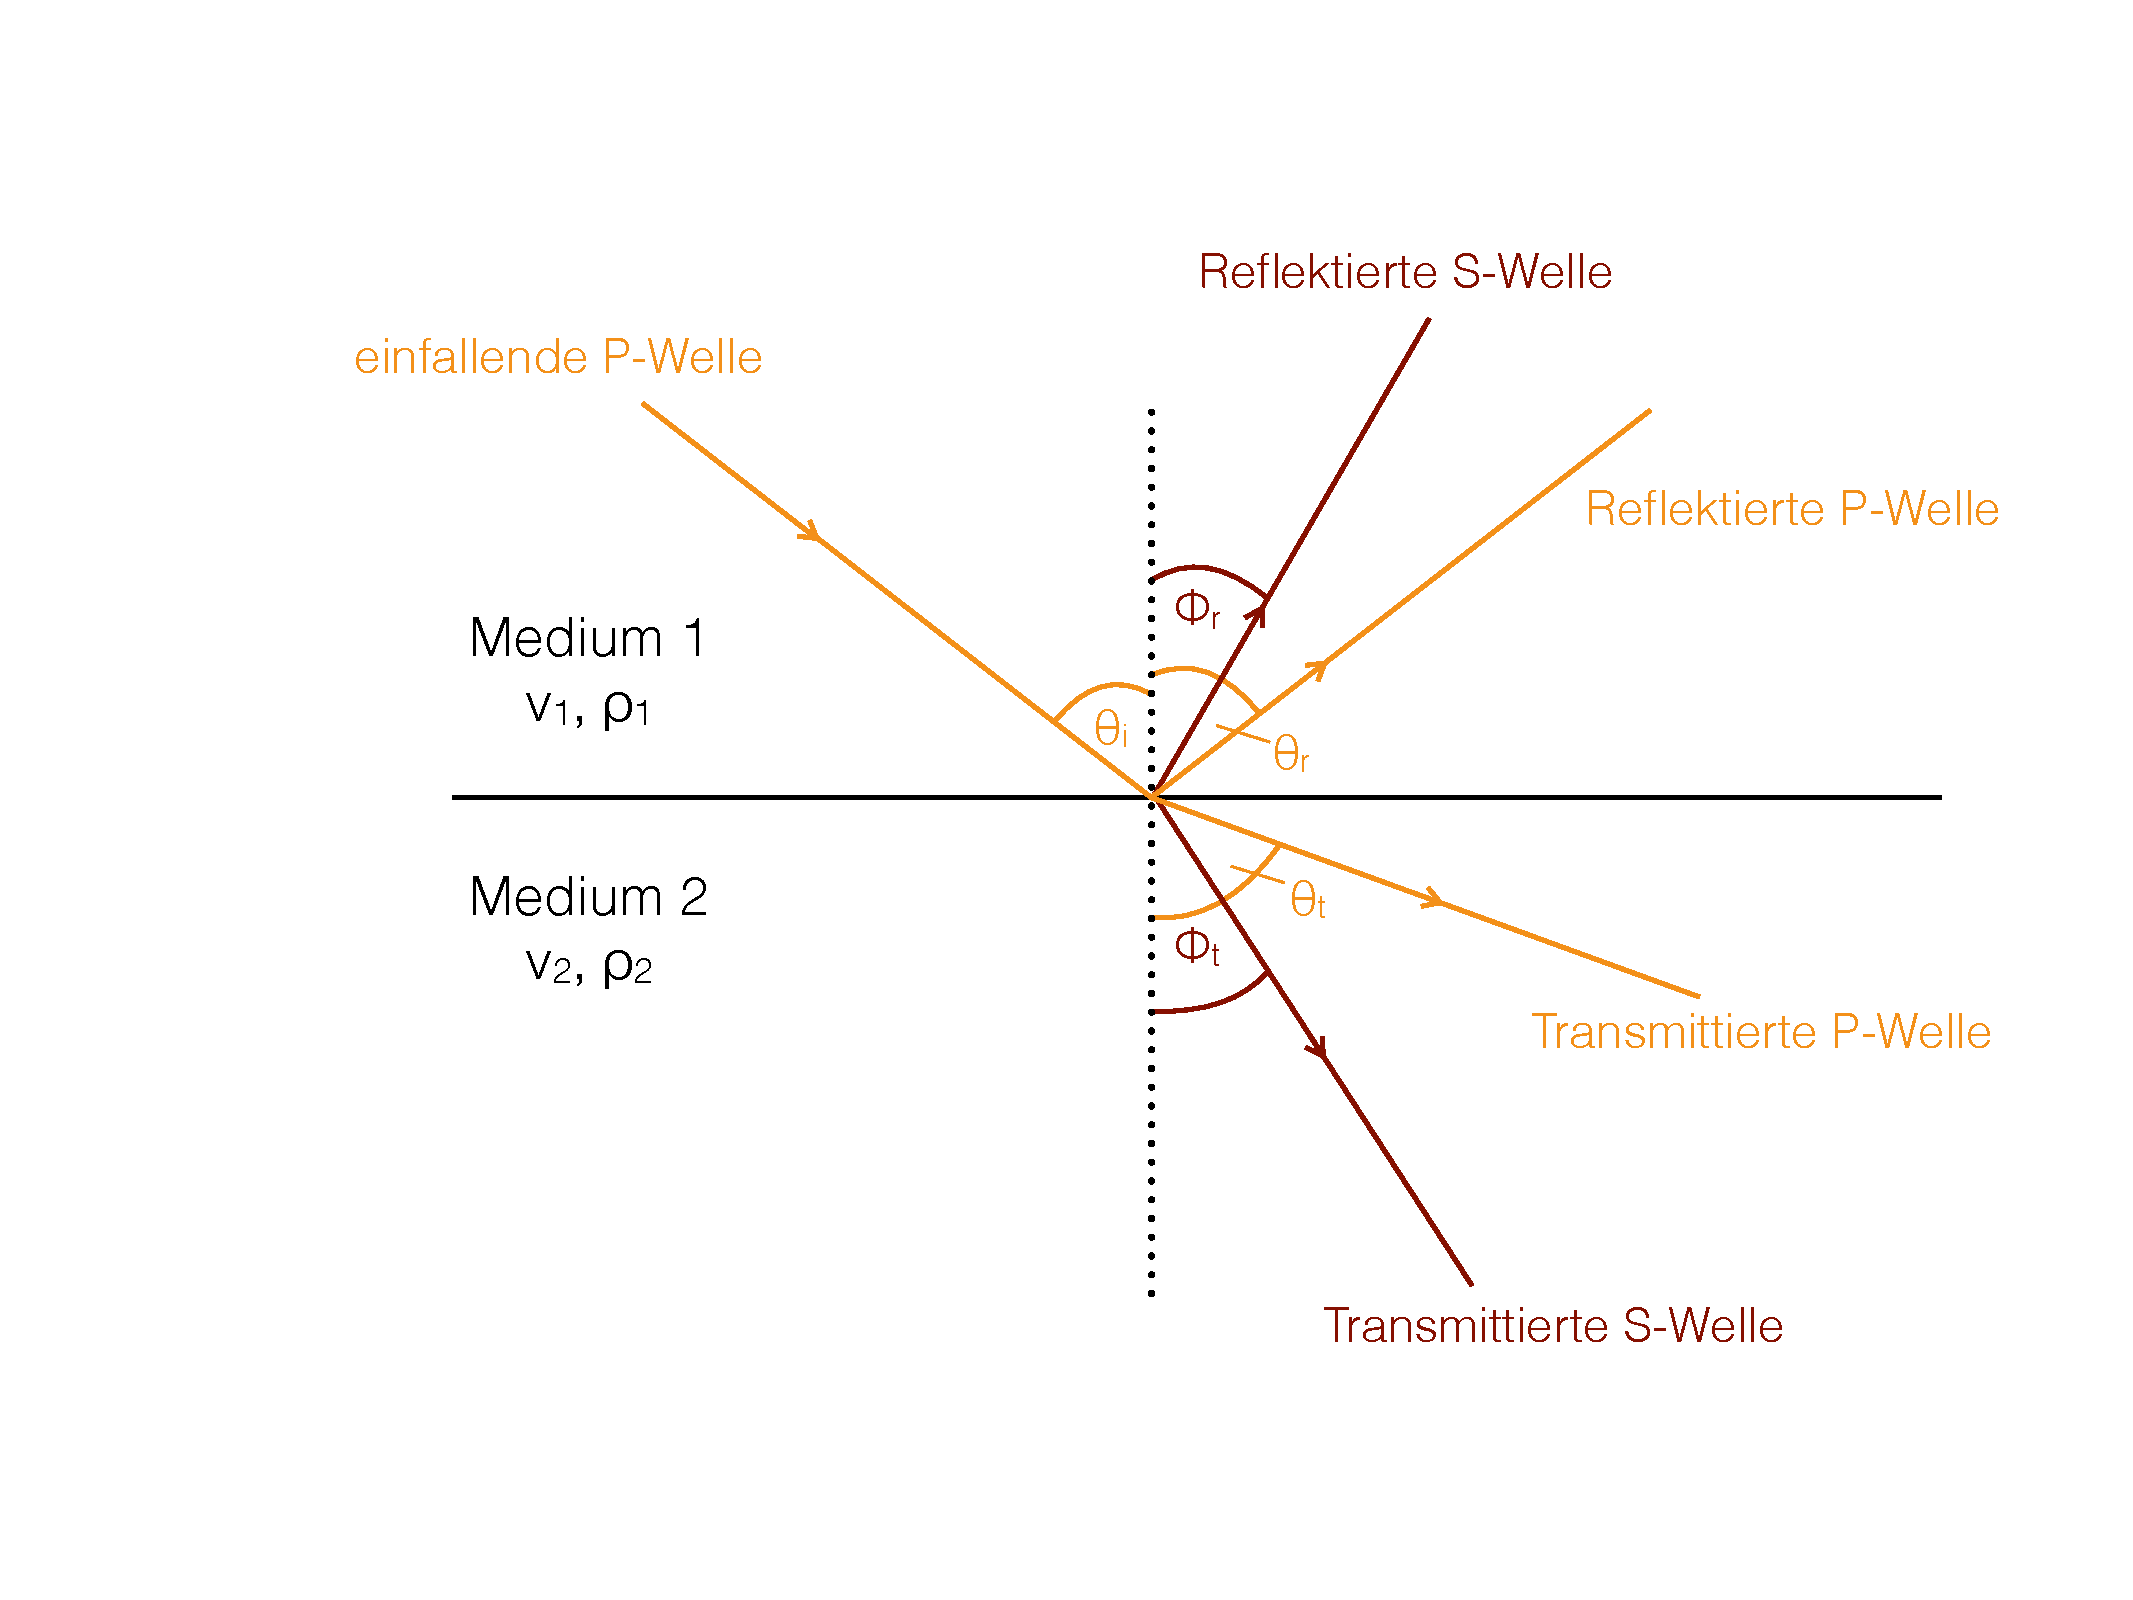
\includegraphics[width = \textwidth]{SeismikBilder/ReflexionTransmission}
\end{figure}

\begin{equation*}
	\frac{sin(\theta_{\text{i}})}{v_{\text{p}_1}} = \frac{sin(\theta_{\text{r}})}{v_{\text{p}_1}} = \frac{sin(\theta_{\text{t}})}{v_{\text{p}_2}} = \frac{sin(\phi_{\text{r}})}{v_{\text{s}_1}} = \frac{sin(\phi_{\text{t}})}{v_{\text{s}_2}}
\end{equation*}


\subsection{Refraktion und kritischer Winkel}
Auch die Refraktion lässt sich einfach mit Hilfe des Snellius'schen Brechungsgesetz berechnen.

\begin{figure}[H]
	\centering
	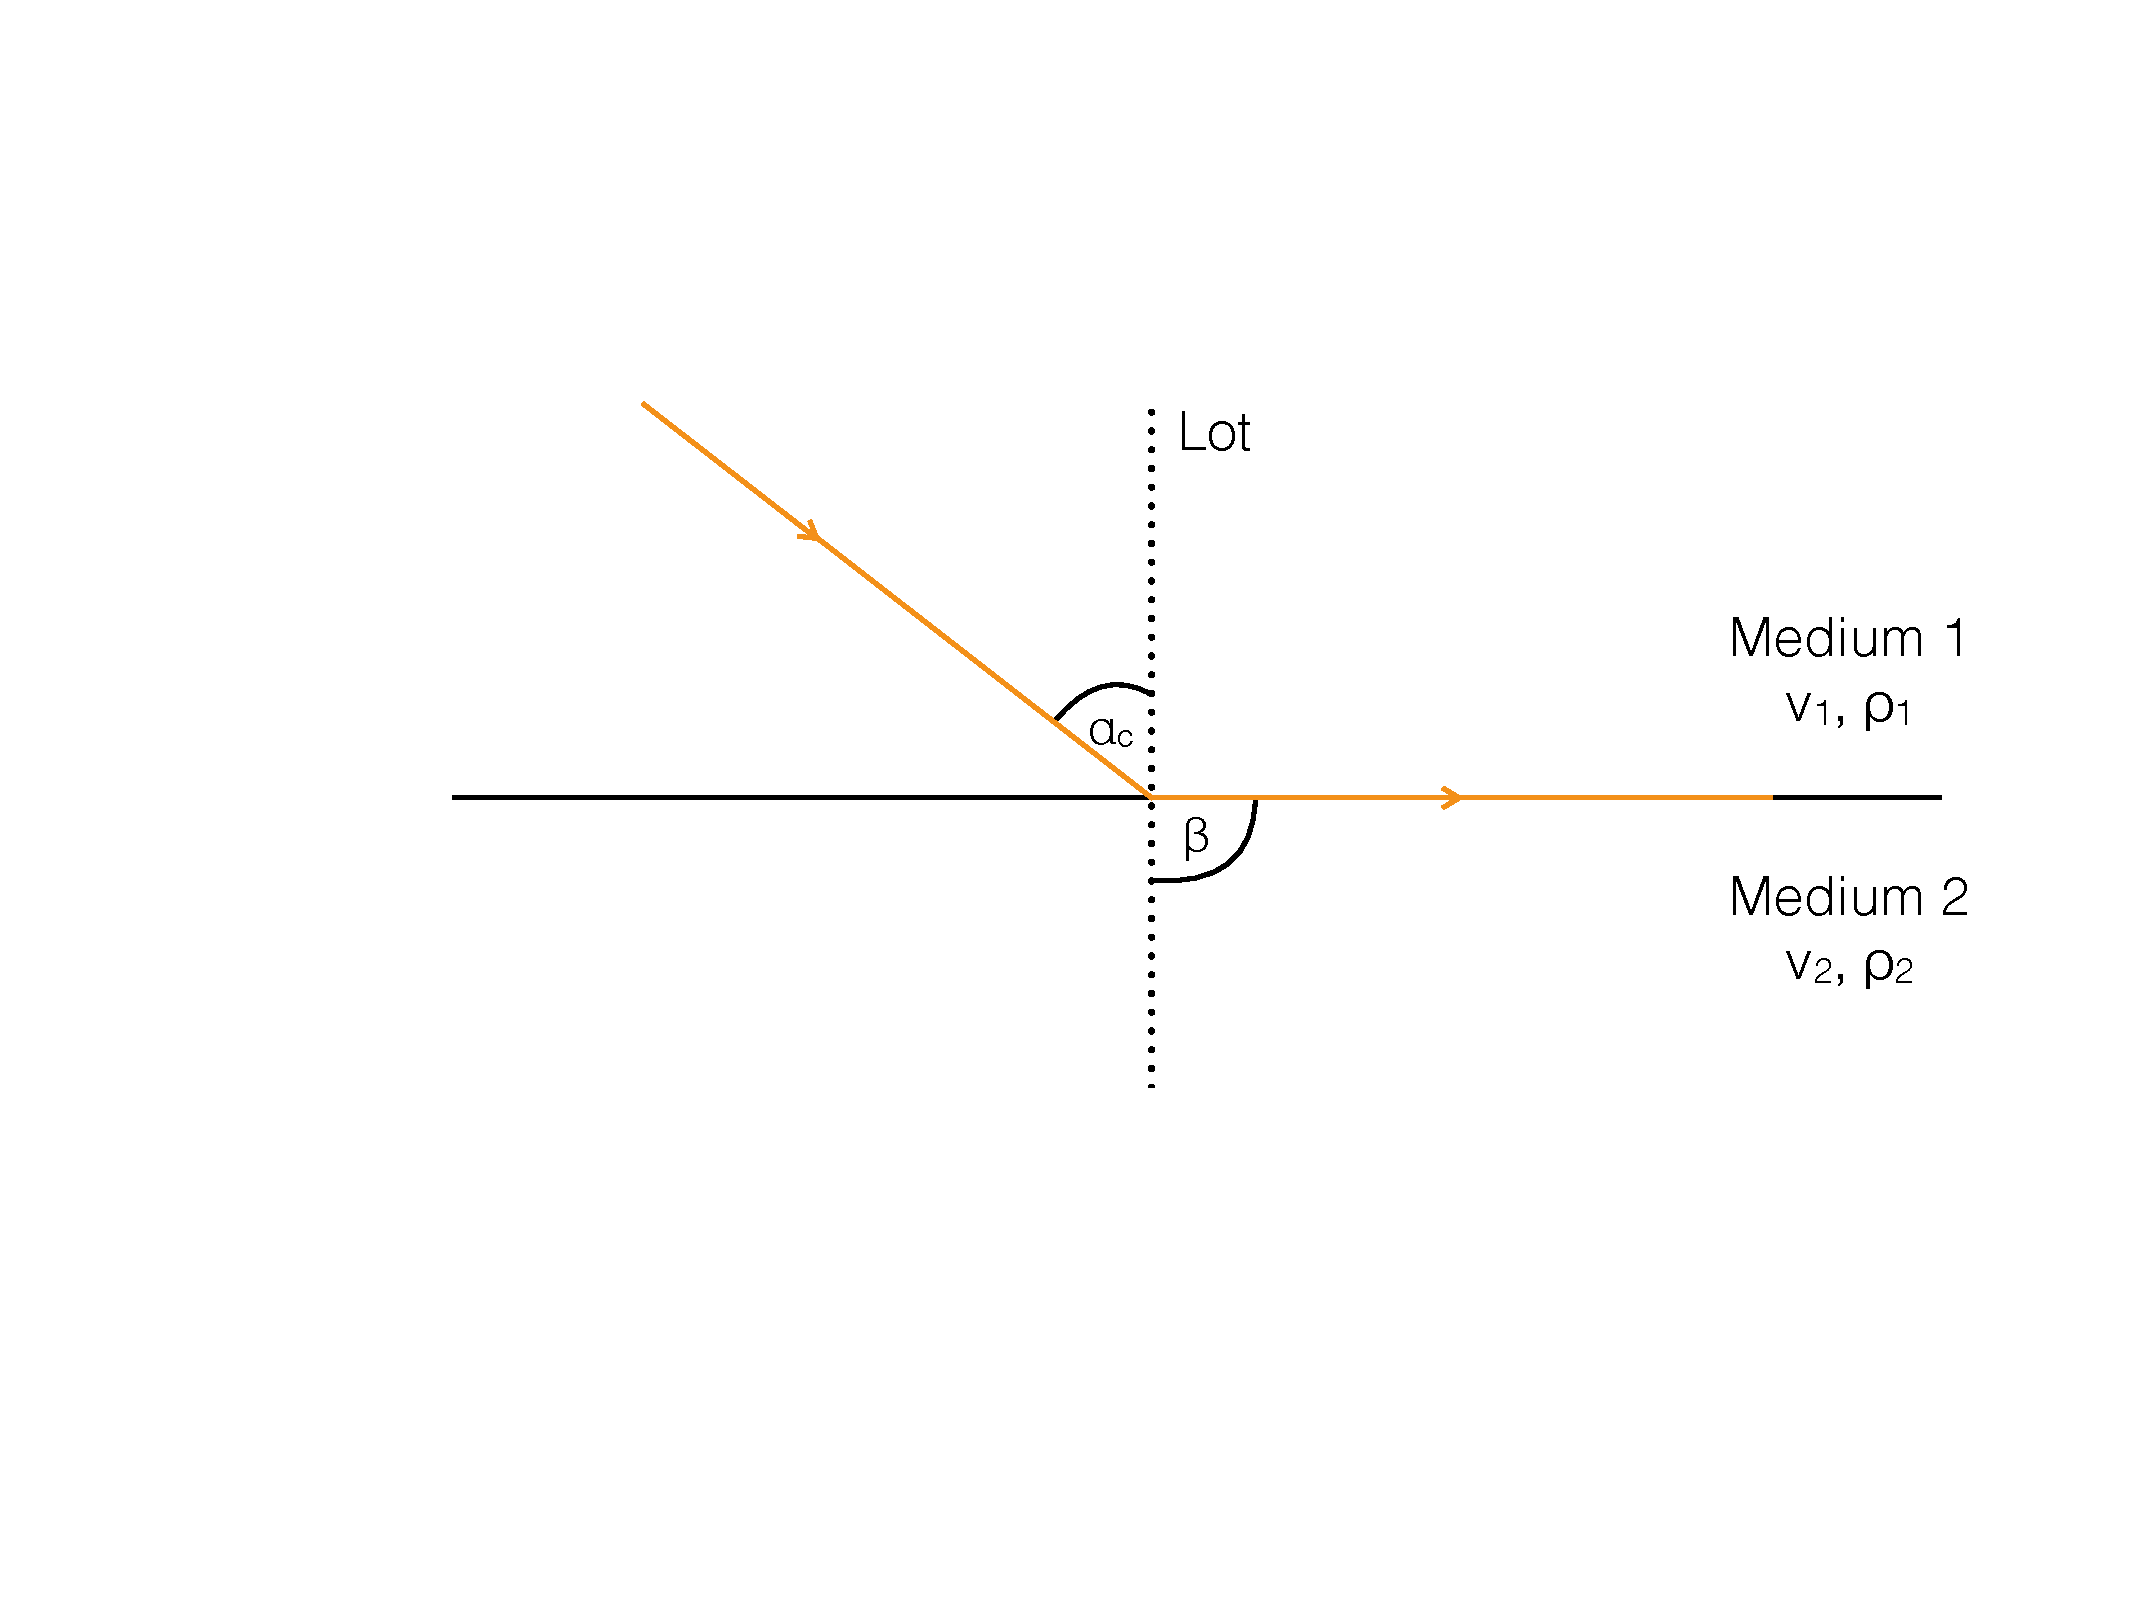
\includegraphics[width = \textwidth]{SeismikBilder/Refraktion}
\end{figure}

\begin{equation*}
	\frac{sin(\alpha)}{v_1} = \frac{sin(\beta)}{v_2} = \frac{1}{v_2} \quad \Rightarrow \quad sin(\alpha) = sin(i_c) = \frac{v_1}{v_2}
\end{equation*}
Dabei ist $i_c$ der \textbf{kritische Winkel}. Fällt die Welle unter dem kritischen Winkel auf die Schichtgrenze, wird die Welle also refraktiert und verläuft entlang der Grenze.


\subsection{Zusammenhang Brechungsgesetz und Wellengeschwindigkeit}
Bei jeder Gesteinsgrenze mit Übergang von einem weniger dichten zu einem dichteren Gestein nimmt die Ausbreitungsgeschwindigkeit einer seismischen Welle zu. Entsprechend ist eine Abnahme der Geschwindigkeit im umgekehrten Fall zu beobachten. Da die Dichte der Gesteine zum Erdinnern hin zunimmt, nimmt auch die Geschwindigkeit einer Welle entsprechend zu. Nach dem Snellius'schen Brechungsgesetz wird eine seismische Welle also mit zunehmender Tiefe vom Lot weg gebrochen. Je näher sie wieder an die Erdoberfläche kommt demnach zum Lot hin gebrochen. Dies erklärt den typischen bogenförmigen Verlauf einer seismischen Welle. Erreicht eine solche Welle wieder die Erdoberfläche, wird sie \textbf{Tauchwelle} genannt.


\begin{figure}[H]
	\centering
	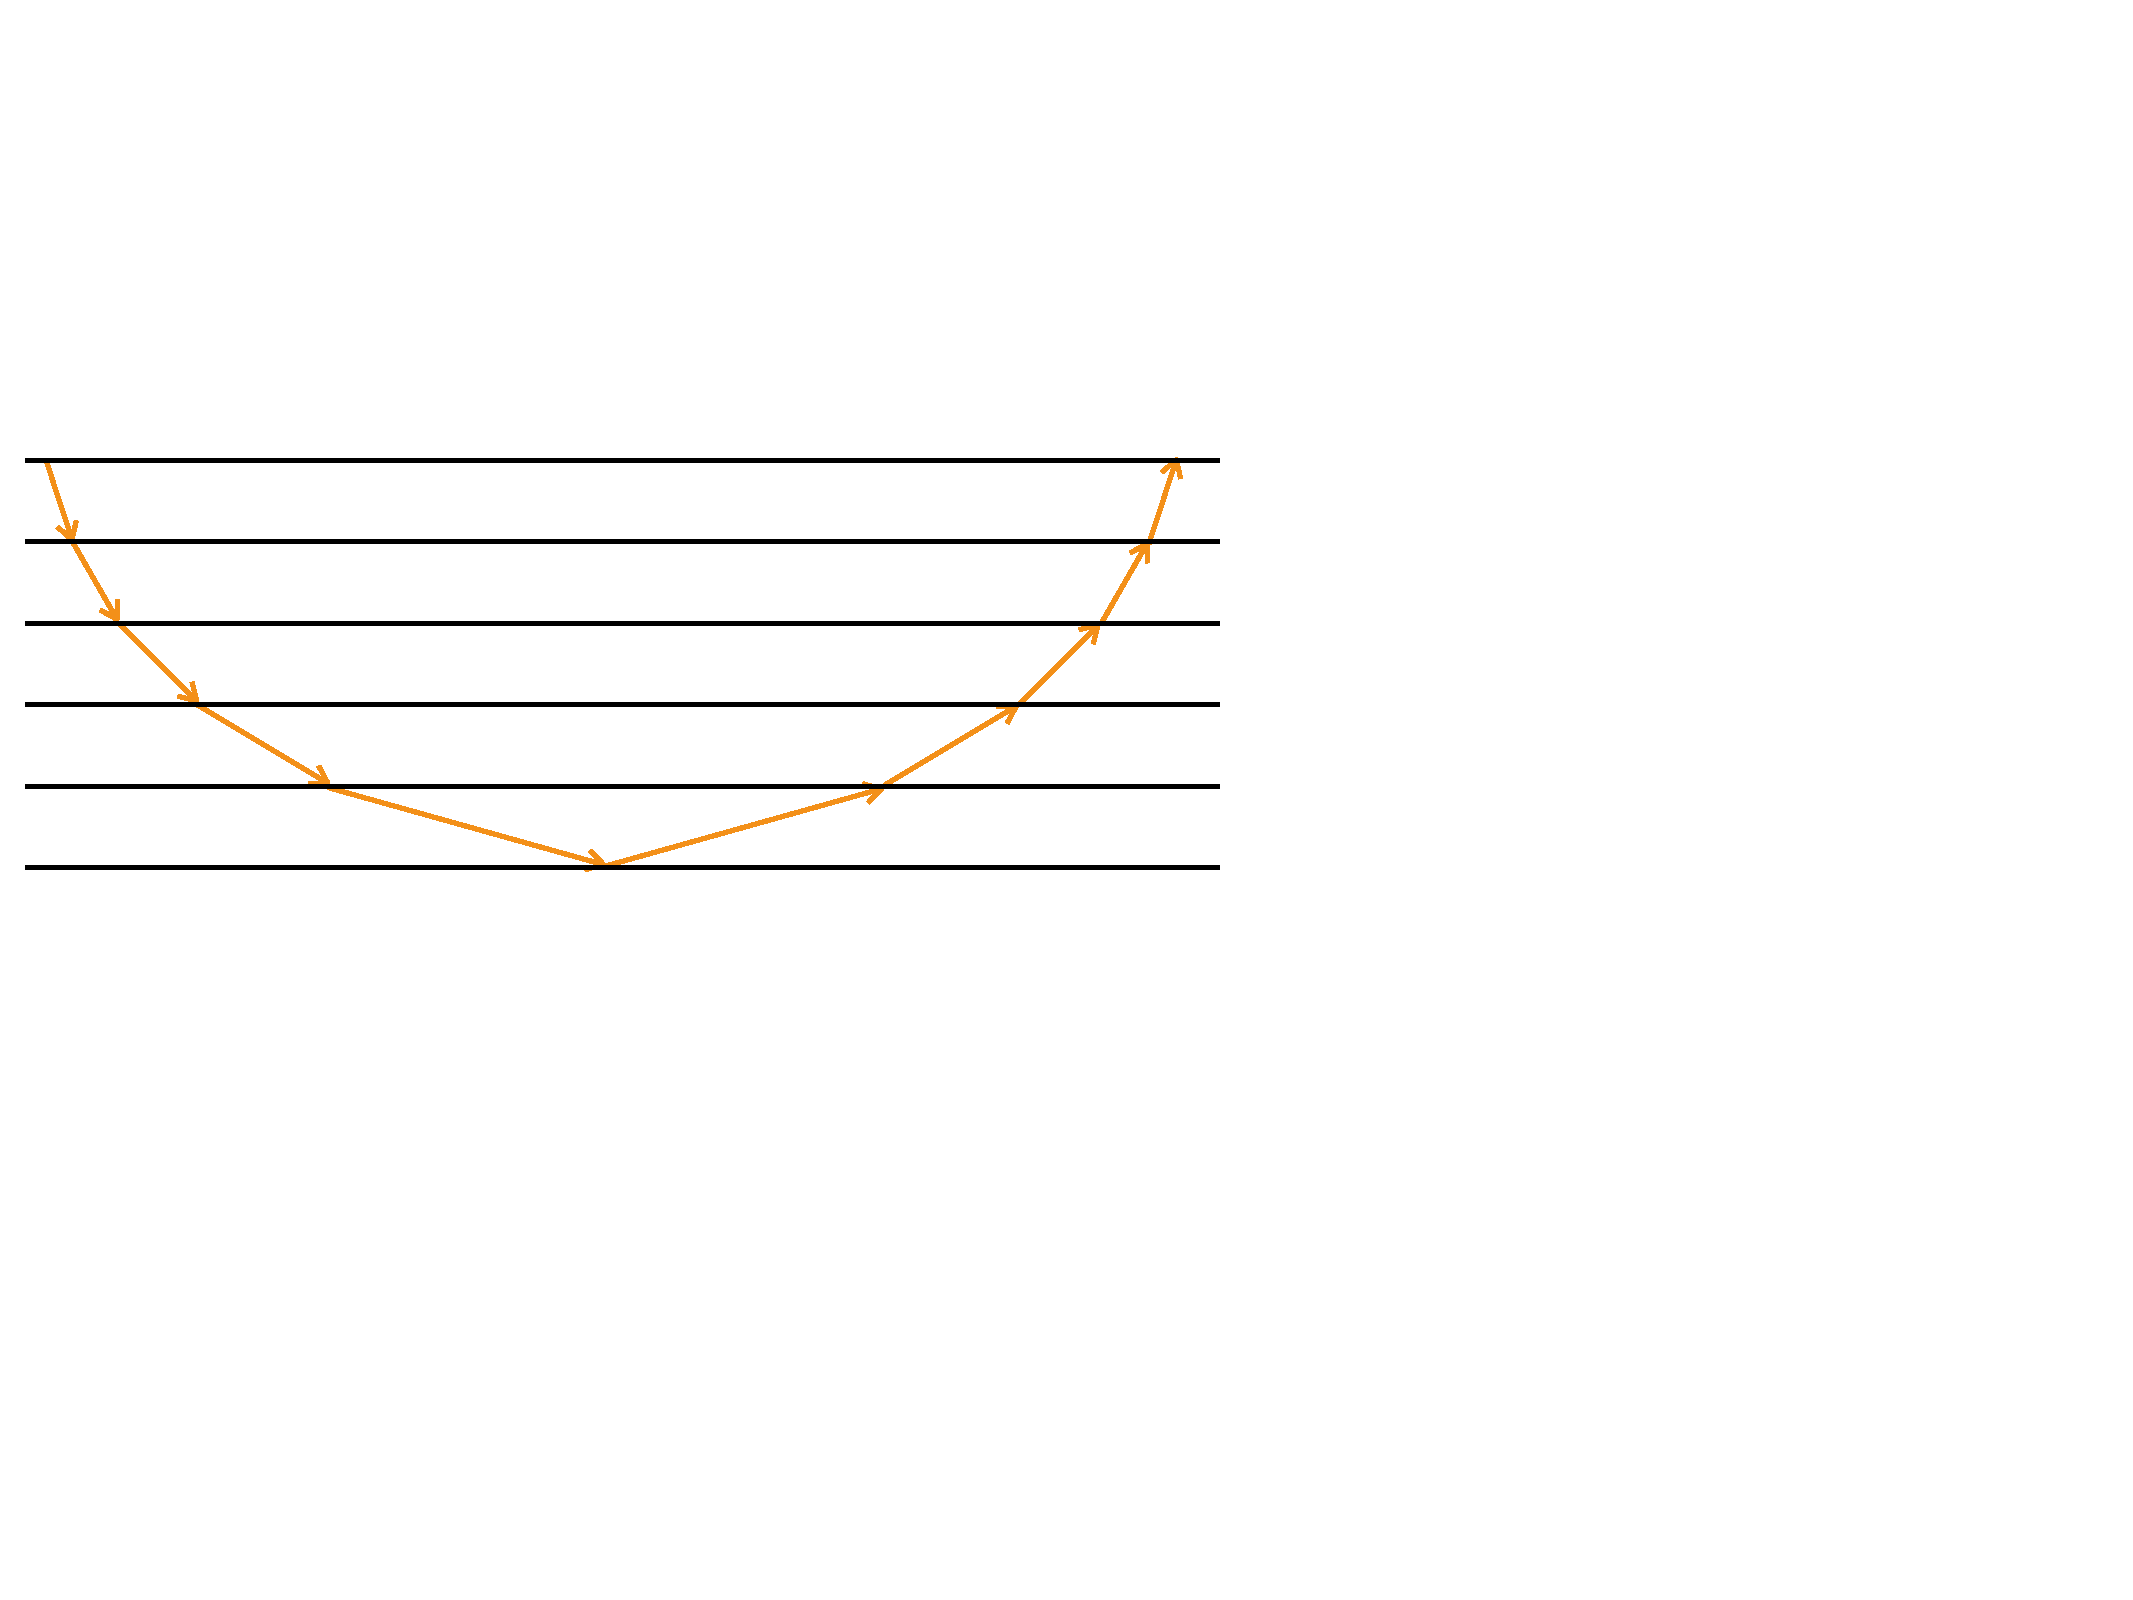
\includegraphics[width = \textwidth]{SeismikBilder/Tauchwelle}
\end{figure}


\section{Zeitmittelgleichung}
In der seismischen Geophysik ist die Lauftzeit und damit die Geschwindigkeit einer Welle im Untergrund sehr wichtig. Bei den obigen Berechnungen sind wir davon ausgegangen, dass die einzelnen Schichten homogen sind. Dies lässt sich aber nicht immer so annähern. 

Eine Möglichkeit, die Geschwindigkeiten abzuschätzen, ist die Zeitmittelgleichung. Diese verrechnet die einzelnen Materialgeschwindigkeiten aus denen sich der Untergrund zusammensetzt. 

Um diese Gleichung aufstellen zu können, wird ein vereinfachtes Gesteinsmodell angenommen: 

\begin{figure}[H]
	\centering
	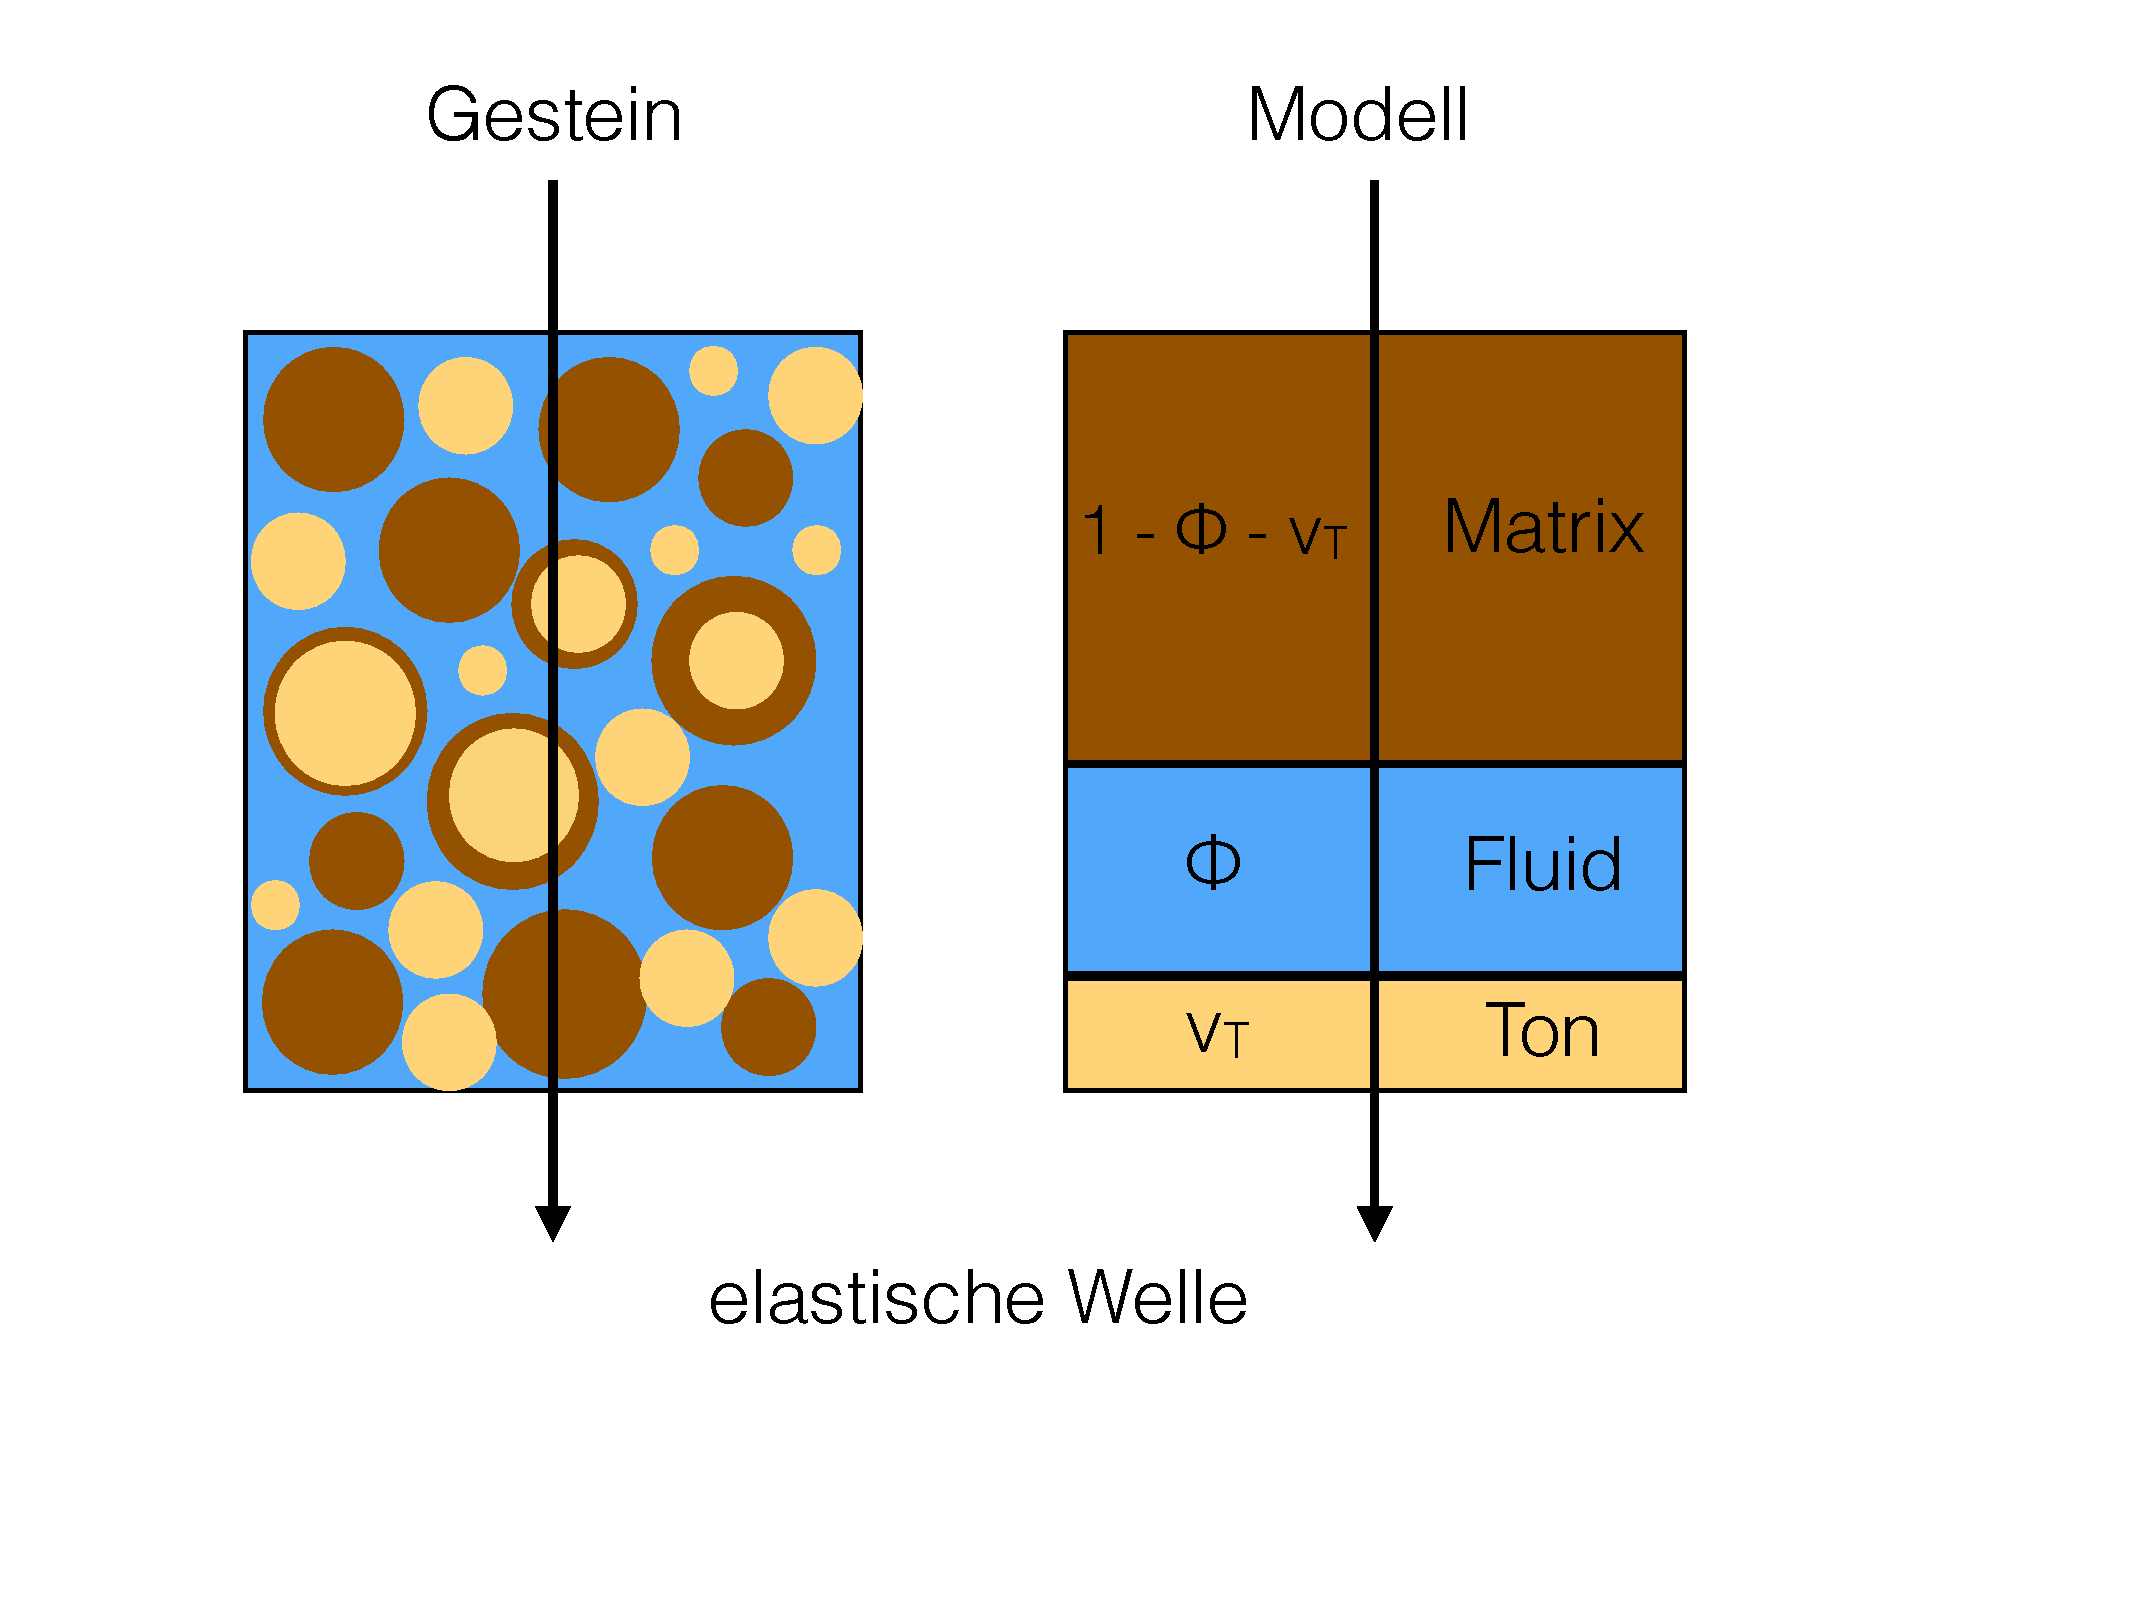
\includegraphics[width = \textwidth]{SeismikBilder/Zeitmittelgleichung}
\end{figure}

\begin{itemize}
	\item volumenproportionale, ebene Platten für jeden Bestandteil
	\item keine Wechselwirkungen zwischen den Materialien
	\item Tonkorrektur
\end{itemize}

Die Zeitmittelgleichung ergibt sich aus der Laufzeitgleichung der Welle \begin{equation*}
	T = T_{\text{Matrix}} + T_{\text{Fluid}} + T_{\text{Ton}}
\end{equation*}

Da die Laufzeit $T$ umgekehrt propotional zu $1/v$ ist, ergibt sich: \begin{equation*}
	\frac{1}{v_{\text{eff}}} = \frac{1 - \phi - v_{\text{T}}}{v_{\text{Matrix}}} + \frac{\phi}{v_{\text{Fluid}}} + \frac{v_{\text{T}}}{v_{\text{Ton}}}
\end{equation*}

\begin{tabular}{ll}
	$v_{\text{eff}}$ & effektive Ausbreitungsgeschwindigkeit im Gestein \\
	$v_{\text{Matrix}}$ & mittlere Ausbreitungsgeschwindigkeit in den Matrixbestandteilen \\
	$v_{\text{Fluid}}$ & mittlere Ausbreitungsgeschwindigkeit in den Fluiden/Gasen \\
	$v_{\text{Ton}}$ & mittlere Ausbreitungsgeschwindigkeit in den Tonbestandteilen \\
	$\phi$ & Porosität (relativer Volumenanteil der Gase/Fluide) \\
	$1 - \phi - v_{\text{T}}$ & relativer Volumenanteil der Matrix \\
	$v_{\text{T}}$ & relativer Volumenanteil des Tons
\end{tabular}

\section{Ausblick}
Seismische Wellen lassen sich für geophysikalische Messungen nutzen. Sie werden durch beispielsweise einen Hammerschlag auf die Erdoberfläche (\textbf{Hammerschlagseismik}) künstlich erzeugt und mit speziellen Messgeräten (\textbf{Geophone}) gemessen. Die gemessenen Daten lassen Rückschlüsse auf die Struktur des Untergrundes zu. Die nächsten beiden Kapitel beschäftigen sich mit zwei verschiedenen Messverfahren auf Grundlage der Seismik.  






	\chapter{Refraktionsseismik}
In diesem Kapitel beschäftigen wir uns mit refraktierten seismischen Wellen. Diese Wellen laufen entlang der Schichtgrenze und strahlen konstant neue Wellen unter dem kritischen Winkel zurück zur Erdoberfläche. Eine solche Welle tritt auf, wenn eine seismische Welle unter dem kritischen Winkel auf die Schichtgrenze trifft. Weiterhin muss dabei die Geschwindigkeit nach unten hin zunehmen. Die refraktierte Welle wird im Allgemeinen auch als \textbf{Kopfwelle} bezeichnet. 

Durch einen Hammerschlag, eine kleine Explosion oder andere Quellen werden an der Oberfläche oder wenige Meter im Erdinnern künstlich seismische Wellen erzeugt. Deren Ausbreitung wird an der Oberfläche mit Hilfe von Geophonen aufgezeichnet. Diese Sensoren sind entlang einer festen Linie (\textbf{Profillinie}) in gleichmäßigem Abstand ausgelegt. Die Abstände zwischen den Messgeräten können wenige Meter bis mehrere Kilometer betragen. Die Gesamtlänge der Profillinie ist zwischen einige zehn Meter bis mehr als 100 Kilometer lang, je nach gewünschter Tiefe der Untersuchung. 

Aus den gemessenen Daten wird ein \textbf{Laufzeitdiagramm} erstellt und ausgewertet. Dabei wird besonders die refraktierte Welle betrachtet. Das Ergebnis dieser Auswertung ist ein Untergrundmodell, welches die einzelnen Schichten mit ihrer jeweiligen Wellengeschwindigkeit zeigt.  

Anwendung finden refraktionsseismische Verfahren beispielsweise in geologischen Erkundungen der Erdkruste und des oberen Erdmantels, wie z.B. die Ermittlung der Tiefe einer Gebirgswurzel.   

\section{Der söhlige Zweischichtfall}
Um die refraktionsseismischen Verfahren zu verstehen, beginnen wir mit dem einfachsten Fall. Der zu untersuchende Untergrund hat eine Schichtgrenze, die horizontal (\textbf{söhlig}) verläuft. Unser Ziel dabei ist die Berechnung der Tiefe der Schichtgrenze (\textbf{Mächtigkeit}) und die Ausbreitungsgeschwindigkeiten in beiden Schichten.

\subsection{Strahlenwege und Laufzeitgleichungen}
Zu Beginn betrachten wir einmal den Verlauf der Wellenstrahlen im Untergrund und deren Laufzeitgleichungen. Letztere lassen sich durch einfache geometrische Überlegungen herleiten. 

\begin{figure}[H]
	\centering
	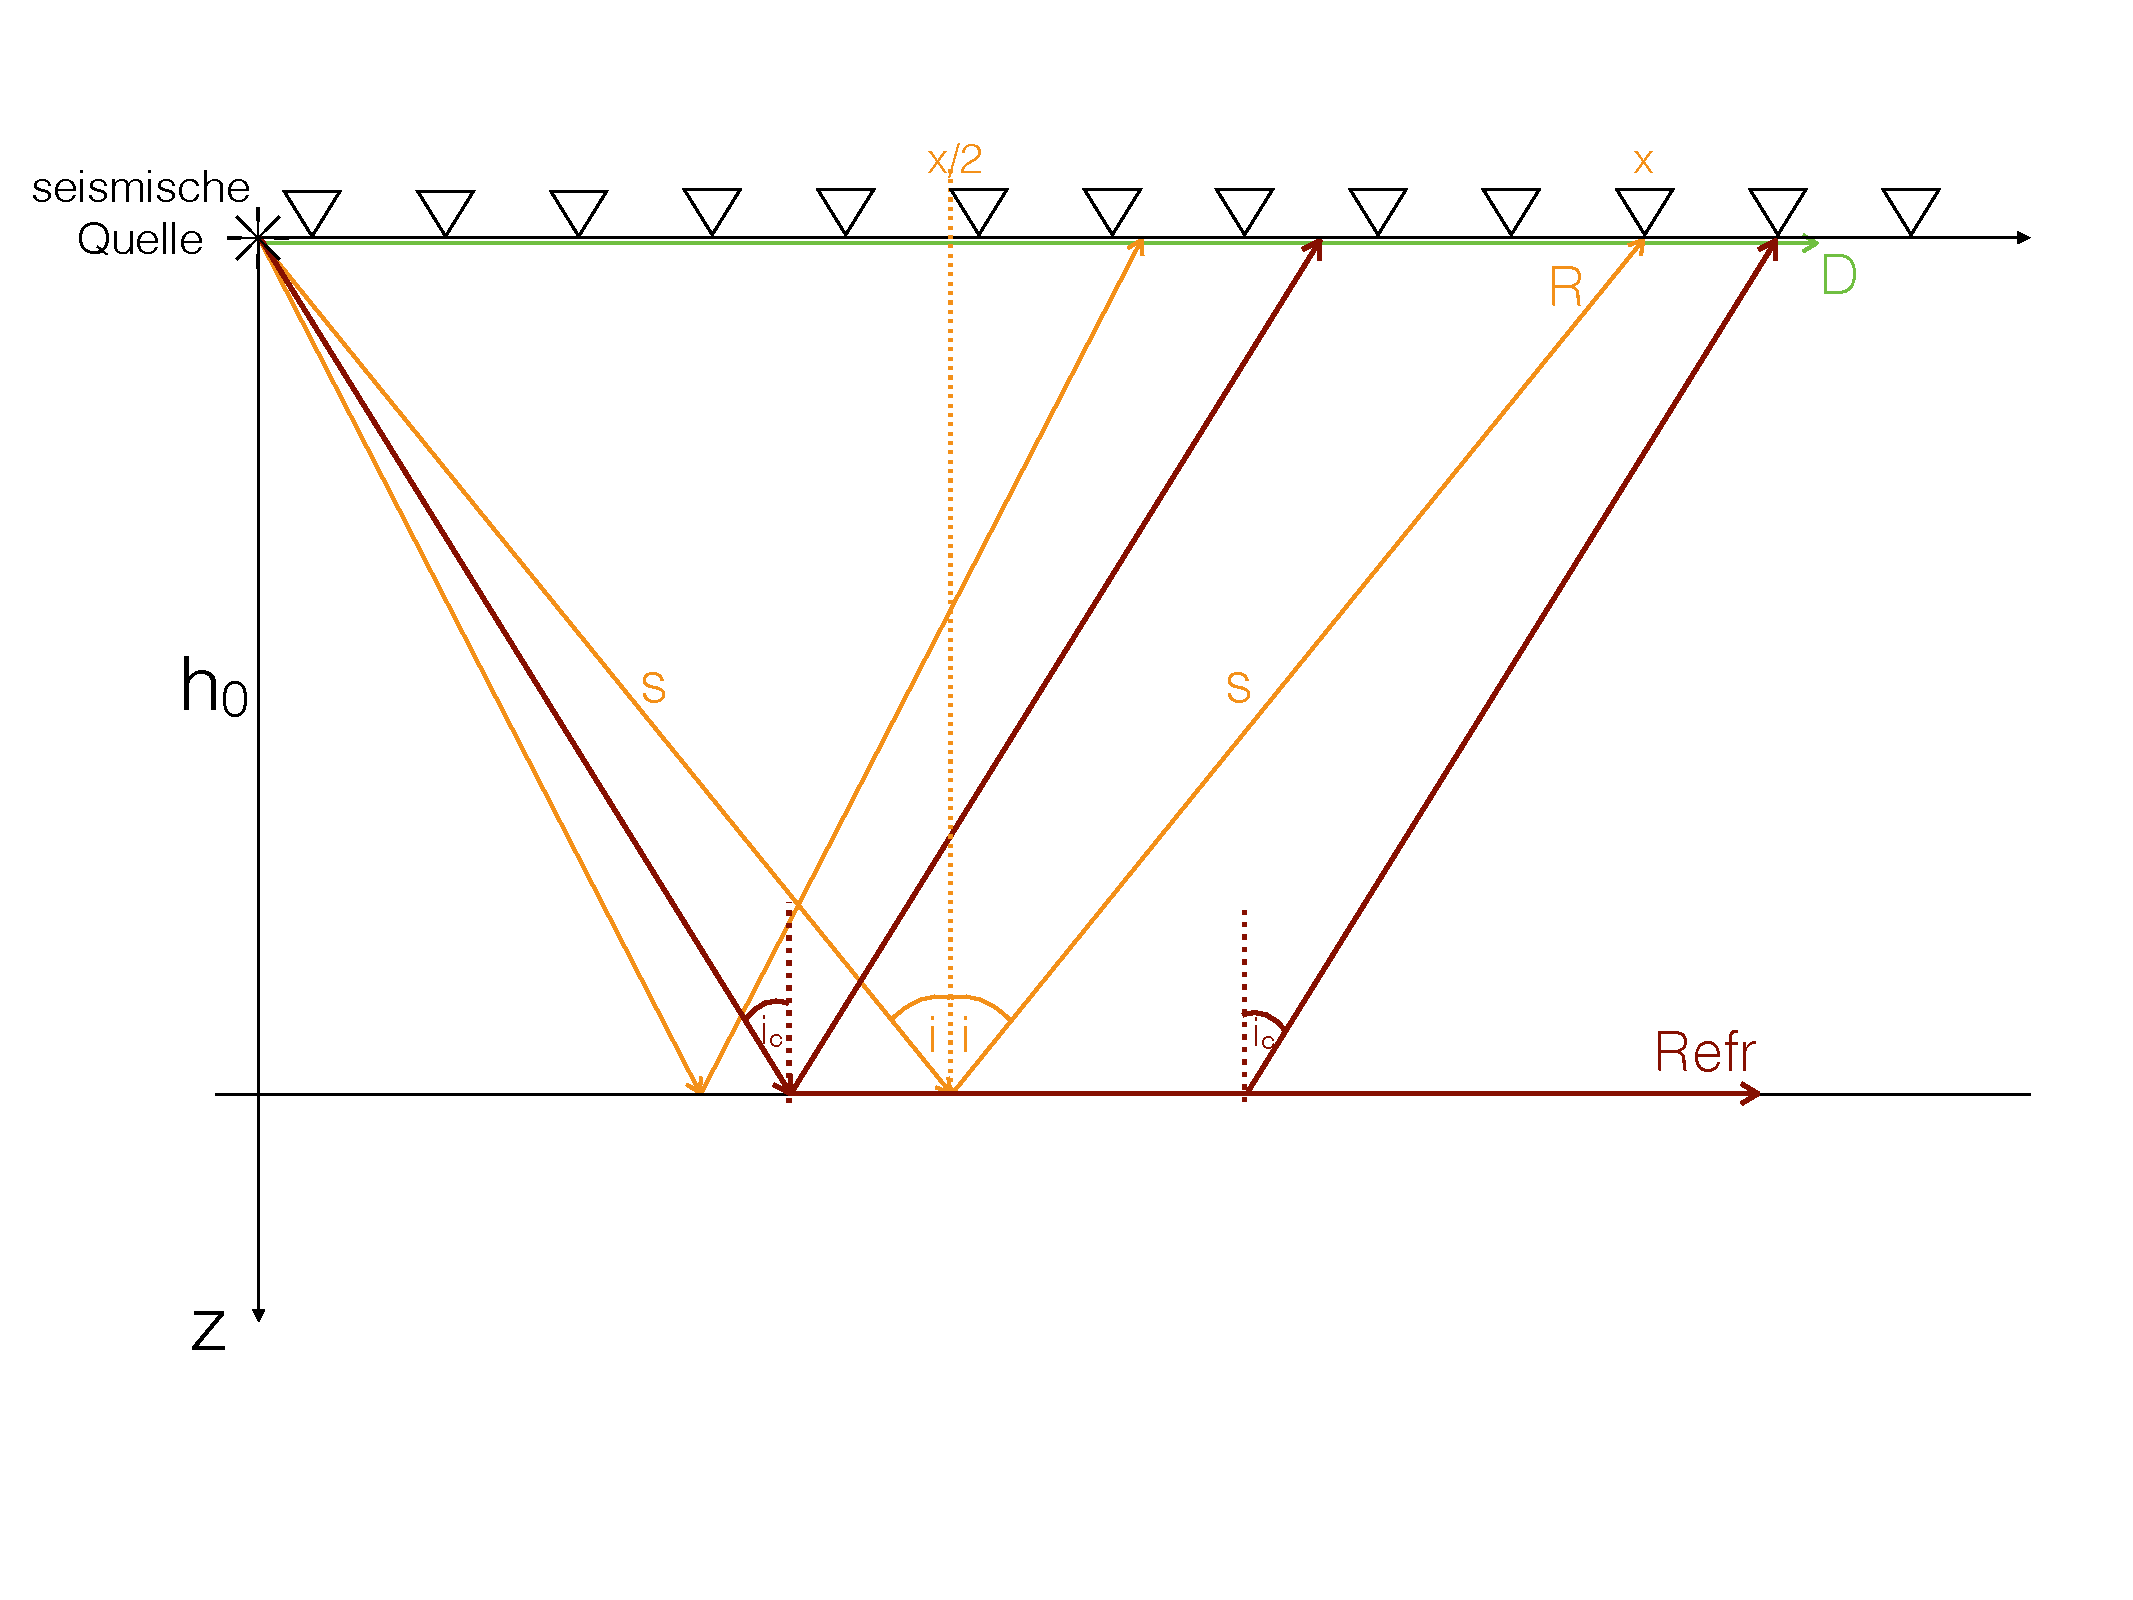
\includegraphics[width = \textwidth]{RefraktionsseismikBilder/soehliger2SchichtFallStrahlen}
\end{figure}


\subsubsection{Direkte Welle (D)}
Diese Welle bewegt sich mit konstanter Geschwindigkeit direkt unter der Erdoberfläche fort. Die Zeit bis zum Antreffen an Punkt $x$ berechnet sich so: \begin{equation*}
	t_{\text{D}} = \frac{x}{v_0}
\end{equation*}

\subsubsection{Reflektierte Welle (R)}
Die Wellenstrahlen werden an der Grenzfläche reflektiert. Es gilt "`Einfallswinkel = Ausfallswinkel"'. Ihre Laufzeit lässt sich folgendermaßen berechnen: \begin{equation*}
	t_{\text{R}} = \frac{2 \cdot s}{v_0} = \frac{2 \cdot \sqrt{\left( \frac{x}{2} \right) ^2 + h_0^2}}{v_0}
\end{equation*}
Um den Wurzelterm zu vereinfachen, quadriert man die gesamte Gleichung: \begin{equation*}
	t_{\text{R}}^2 = \left( \frac{x}{v_0} \right)^2 + \left( \frac{2 \cdot h_0}{v_0} \right) ^2 =  \left( \frac{x}{v_0} \right)^2 + t_0^2
\end{equation*}
Wobei $t_0$ der Ersteinsatz der reflektierten Welle ist.

\subsubsection{Refraktierte Welle (Refr)}
Die Wellenstrahlen treffen unter dem kritischen Winkel auf die Grenzfläche und verlaufen entlang dieser. Dabei werden kontinuierlich neue Wellenstrahlen unter dem kritischen Winkel zur Erdoberfläche zurück gestrahlt. Die Laufzeit der refraktierten Welle berechnet sich so: \begin{equation*}
	t_{\text{Refr}} = \frac{2 \cdot h_0 \cdot cos(i_c)}{v_0} + \frac{x}{v_1}
\end{equation*}



\subsection{Laufzeitdiagramm}
Die Ergebnisse unserer Messung übertragen wir in ein Diagramm. 

\begin{figure}[H]
	\centering
	\includegraphics[width = \textwidth]{RefraktionsseismikBilder/LaufzeitdiagrammSöhlig}
\end{figure}

Es seinen noch einige Begriffe aus dem Diagramm erklärt: \begin{description}
	\item[kritische Entfernung $x_{\text{c}}$:] Bei dieser Entfernung tritt die refraktierte Welle das erste Mal auf, d.h. sie wird das erste Mal von einem Geophon gemessen. 
	\item[Knickpunkt $x_{\text{k}}$:] An diesem Punkt überholt die refraktierte Welle die direkte Welle.
	\item[Interceptzeit $t_{\text{i}}$:] Diese Zeit bezeichnet den errechneten, theoretischen Ersteinsatz der Kopfwelle.  
\end{description}

\subsection{Auswertung}
Wie bereits erwähnt, interessieren uns die Ausbreitungsgeschwindigkeiten $v_0$ und $v_1$ der Schichten, sowie die Tiefe $h_0$ der Schichtgrenze.

\subsubsection{Wellengeschwindigkeit $v_0$}
Die Ausbreitungsgeschwindigkeit einer seismischen Welle in der oberen Schicht ergibt sich direkt aus der Steigung der direkten Welle: \begin{equation*}
	v_0 = \frac{x}{t_{\text{D}}}
\end{equation*}

\subsubsection{Wellengeschwindigkeit $v_1$}
Die Geschwindigkeit der zweiten Schicht ergibt sich auch sehr einfach aus der Steigung der refraktierten Welle: \begin{equation*}
	v_1 = \frac{\Delta x}{\Delta t_{\text{refr}}}
\end{equation*}

\subsubsection{Schichtmächtigkeit $h_0$: Möglichkeit 1}
Ein Ansatz zur Berechnung von $h_0$ ergibt sich aus der Intercept-Zeit: \begin{equation*}
	t_i = \frac{2 \cdot h_0 \cdot cos(i_c)}{v_0}
\end{equation*}
Diese Gleichung stellen wir nach $h_0$ um: \begin{equation*}
	h_0 = \frac{v_0 \cdot t_{\text{i}}}{2 \cdot cos(i_c)}
\end{equation*}
Wir möchten nun noch den kritischen Winkel in der Gleichung ersetzen. Hierzu verwenden wir den mathematischen Zusammenhang: \begin{equation*}
	cos(i_c) = \sqrt{1 - sin^2(i_c)} 
\end{equation*} 
Weiterhin wissen wir, wie sich der kritische Winkel mit dem Sinus ausdrücken lässt. \begin{equation*}
	sin(i_c) = \frac{v_0}{v_1}
\end{equation*}
Hieraus ergibt sich dann die Formel zur Berechnung von $h_0$: \begin{equation*}
	h_0 = \frac{t_{\text{i}}}{2} \cdot \frac{v_0 \cdot v_1}{\sqrt{v_1^2 - v_0^2}}
\end{equation*}


\subsubsection{Schichtmächtigkeit $h_0$: Möglichkeit 2}
Eine weitere Möglichkeit ist die Berechnung mit Hilfe des Knickpunktes. An dieser Stelle sind die Laufzeit von direkter Welle und refraktierter Welle gleich, also setzen wir die Laufzeitgleichungen gleich: \begin{equation*}
	t_{\text{D}}(x_{\text{k}}) = t_{\text{Refr}}(x_{\text{k}}) \quad \Rightarrow \quad h_0 = \frac{x_{\text{k}}}{2} \cdot \sqrt{\frac{v_1 - v_0}{v_1 + v_0}}
\end{equation*}


\subsubsection{Schichtmächtigkeit $h_0$: Möglichkeit 3}
Die letzte Variante ist die Berechnung aus der $t_0$-Zeit. Die Formel hierfür ergibt sich direkt durch Umstellen: \begin{equation*}
	h_0 = \frac{v_0 \cdot t_0}{2}
\end{equation*}



\section{Der geneigte Zweischichtfall}
Dass die Schichtgrenze exakt horizontal verläuft, ist ein sehr unwahrscheinlicher Fall. In der Regel ist die Schichtgrenze um einen Winkel $\delta$ geneigt. Damit sich die Schichtgeschwindigkeiten dennoch berechnen lassen, werden zwei Messungen durchgeführt. Die eine Messung beginnt an einem Ende der Profillinie, die Zweite am anderen Ende. Erstere Messung nennt man \textbf{Hinschuss} und die zweite Messung entsprechend \textbf{Rückschuss}. Der kritische Winkel der Welle verändert sich durch die Schichtneigung nicht.

\subsection{Strahlenwege}
Auch hier wollen wir uns zunächst einmal den Verlauf der Wellen anschauen. Um die Grafik etwas übersichtlicher zu gestalten, tragen wir nur den Verlauf der Strahlen der refraktierten Welle von Hin- und Rückschuss ein.

\begin{figure}[H]
	\centering
	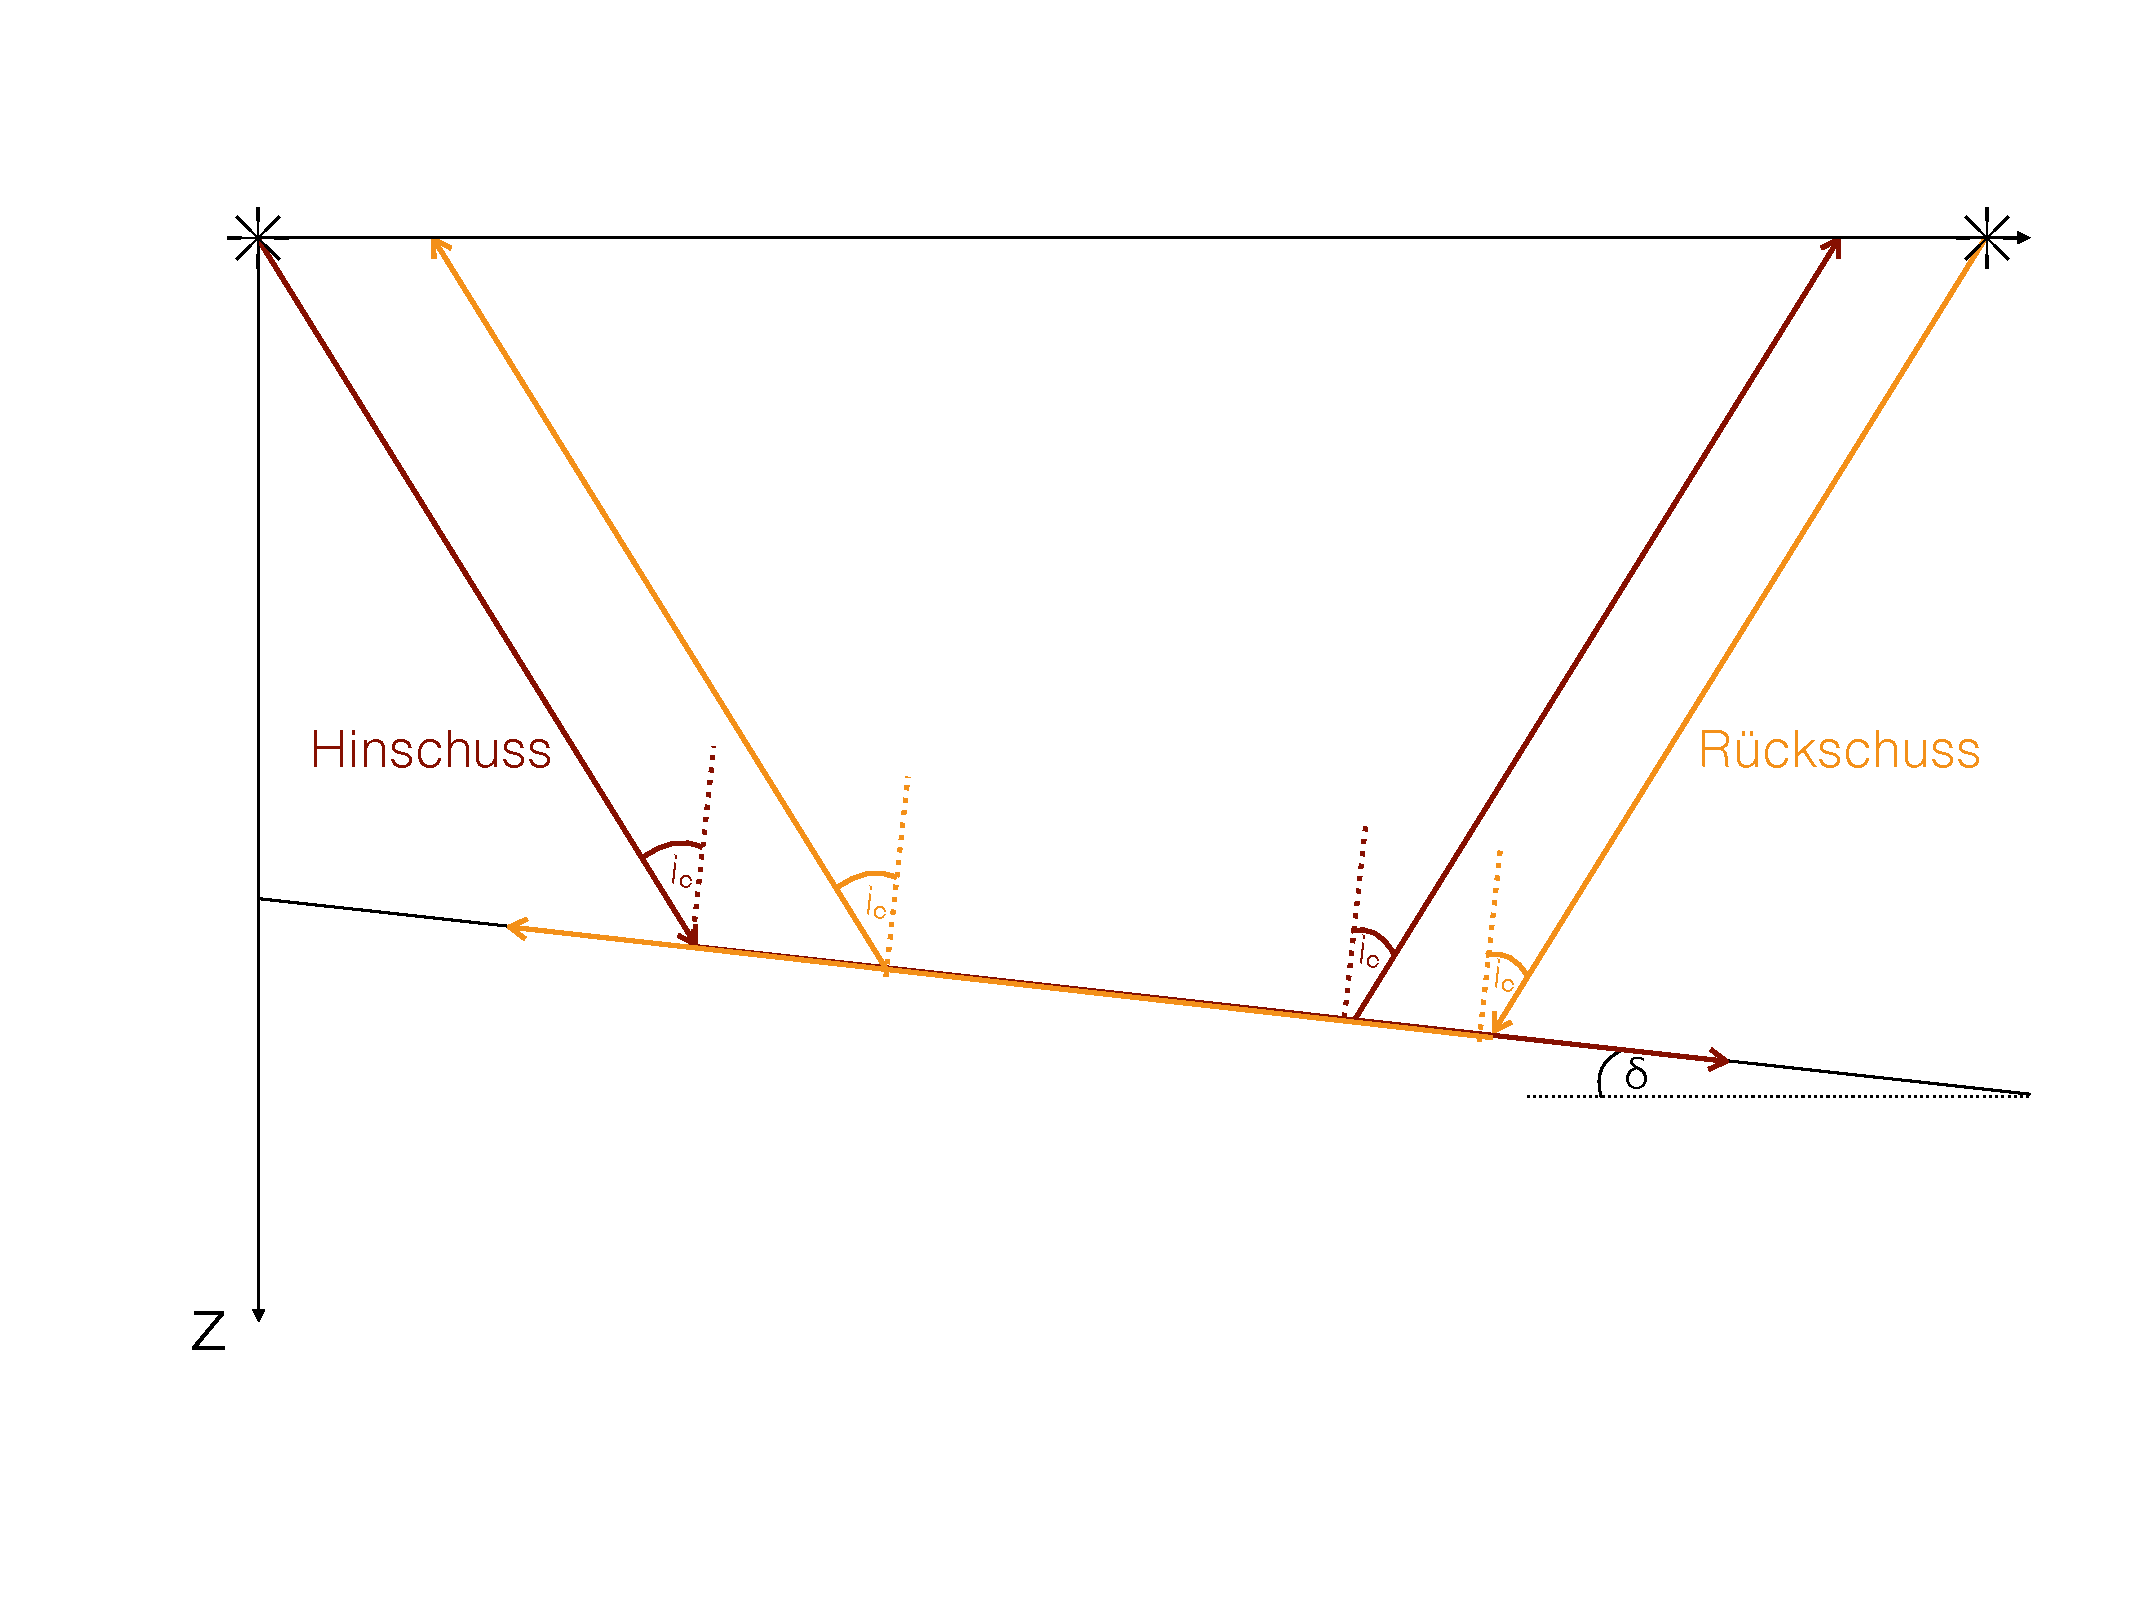
\includegraphics[width = \textwidth]{RefraktionsseismikBilder/geneigteSchichtStrahlen}
\end{figure}


\subsection{Laufzeitdiagramm}
Auch hier übertragen wir die Messergebnisse in ein Diagramm. 

\begin{figure}[H]
	\centering
	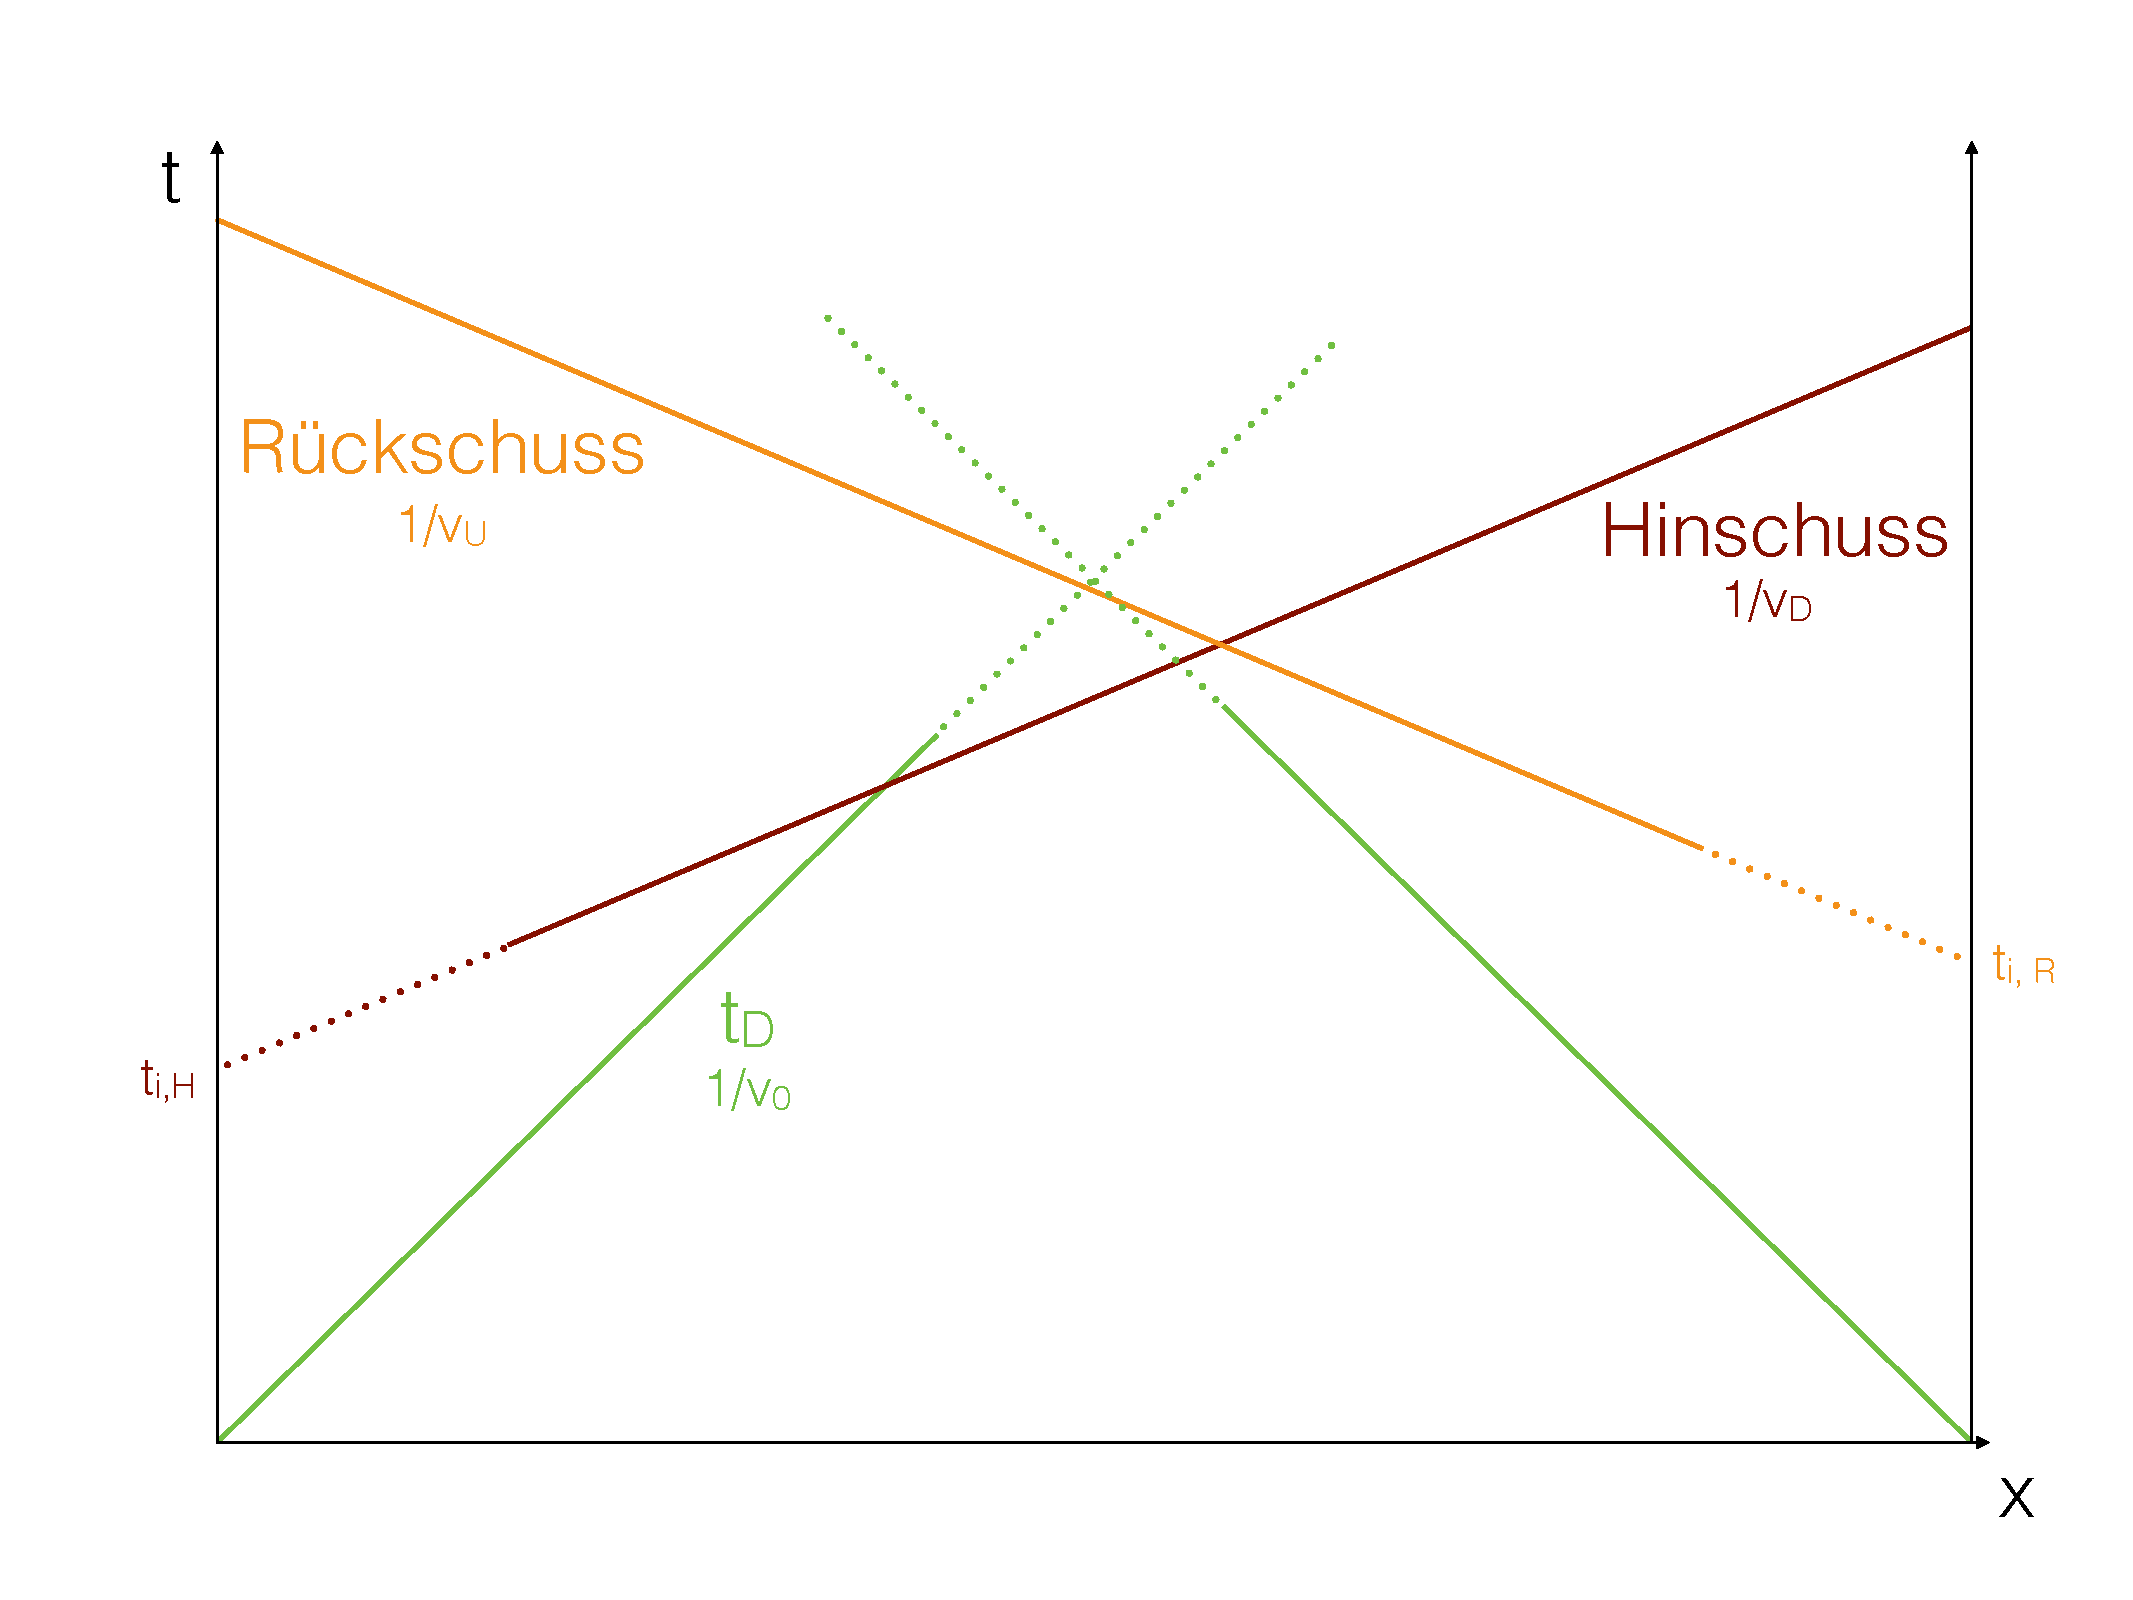
\includegraphics[width = \textwidth]{RefraktionsseismikBilder/LaufzeitdiagrammGeneigt}
\end{figure}

In dieser Grafik haben wir die Wellengeschwindigkeit beim Hinschuss $v_{\text{D}}$ und beim Rückschuss $v_{\text{U}}$ genannt. D und U stehen dabei für "`Down-Dip"' bzw. "`Up-Dip"' Geschwindigkeit. 

Wir benutzen die Steigungen der refraktierten Wellen von Hin- und Rückschuss, um die Schichtgeschwindigkeiten zu berechnen. Im Folgenden sei $v_0$ die Wellengeschwindigkeit in der oberen Schicht und $v_1$ die Geschwindigkeit in der Schicht unter der geneigten Grenzfläche. 

$v_0$ ergibt sich direkt durch Umstellen der Steigungsgleichungen von Up- und Down-Dip: \begin{align*}
		\frac{1}{v_{\text{U}}} &= \frac{sin(i_c - \delta)}{v_0} \\
		\frac{1}{v_{\text{D}}} &= \frac{sin(i_c + \delta)}{v_0}
\end{align*}

$v_1$ ergibt sich wiederum einfach durch den kritischen Winkel: \begin{equation*}
	\frac{1}{v_1} = \frac{sin(i_c)}{v_0}
\end{equation*}

Um $v_0$ hierfür nicht extra berechnen zu müssen, aproximieren wir die Gleichung und drücken sie durch $v_{\text{D}}$ und $v_{\text{U}}$ aus: \begin{equation*}
	\frac{1}{v_1} = \frac{sin(i_c)}{v_0} \approx \frac{sin(i_c + \delta) + sin(i_c - \delta)}{2 v_0} = \frac{1}{2} \left( \frac{1}{v_{\text{U}}} + \frac{1}{v_{\text{D}}} \right)
\end{equation*}





	\chapter{Reflexionsseismik}
In diesem Kapitel wollen wir uns mit einer weiteren geophysikalischen Messmethode aus dem Gebiet der Seismik beschäftigen. Diese Methode nutzt wie die Refraktionsseismik künstlich erzeugte seismische Wellen, wertet aber hauptsächlich die reflektierten Wellen aus. Das Hauptziel einer reflexionsseismischen Messung ist die Lokalisierung von Schichtgrenzen.

Typisch für die Reflexionsseismik ist die riesige Datenmenge, die bei der Messung aufgenommen wird, da die Profillänge meist mehrere zehn Kilometer lang ist. Diese Datenmengen sorgen für eine geringe Mehrdeutigkeit in der Auswertung und macht die Reflexionsseismik damit zur geophysikalischen Messmethode mit der zuverlässigsten Aussage über den Untergrund. Allerdings ist der Kostenaufwand einer solchen Messung enorm hoch. Weiterhin ist die Datenverarbeitung aus Datenauswertung sehr aufwändig und erfordert High-Performance-Computing. 


Die Eindringtiefe liegt in der Regel zwischen 100\,m und 1\,km. Tiefenseismische Messungen dringen jedoch in Tiefen bis zu 100\,km vor.   

Anwendung findet die Reflexionsseismik in Forschungsbereichen zur Rohstoffexploration, Energiegewinnung und Endlagerung.


\section{Zero-Offset-Konfiguration}
Dies ist die einfachste Messkonfiguration für eine reflexionsseismische Messung. Sender um Empfänger stehen hier am gleichen Ort.

\begin{figure}[H]
	\centering
	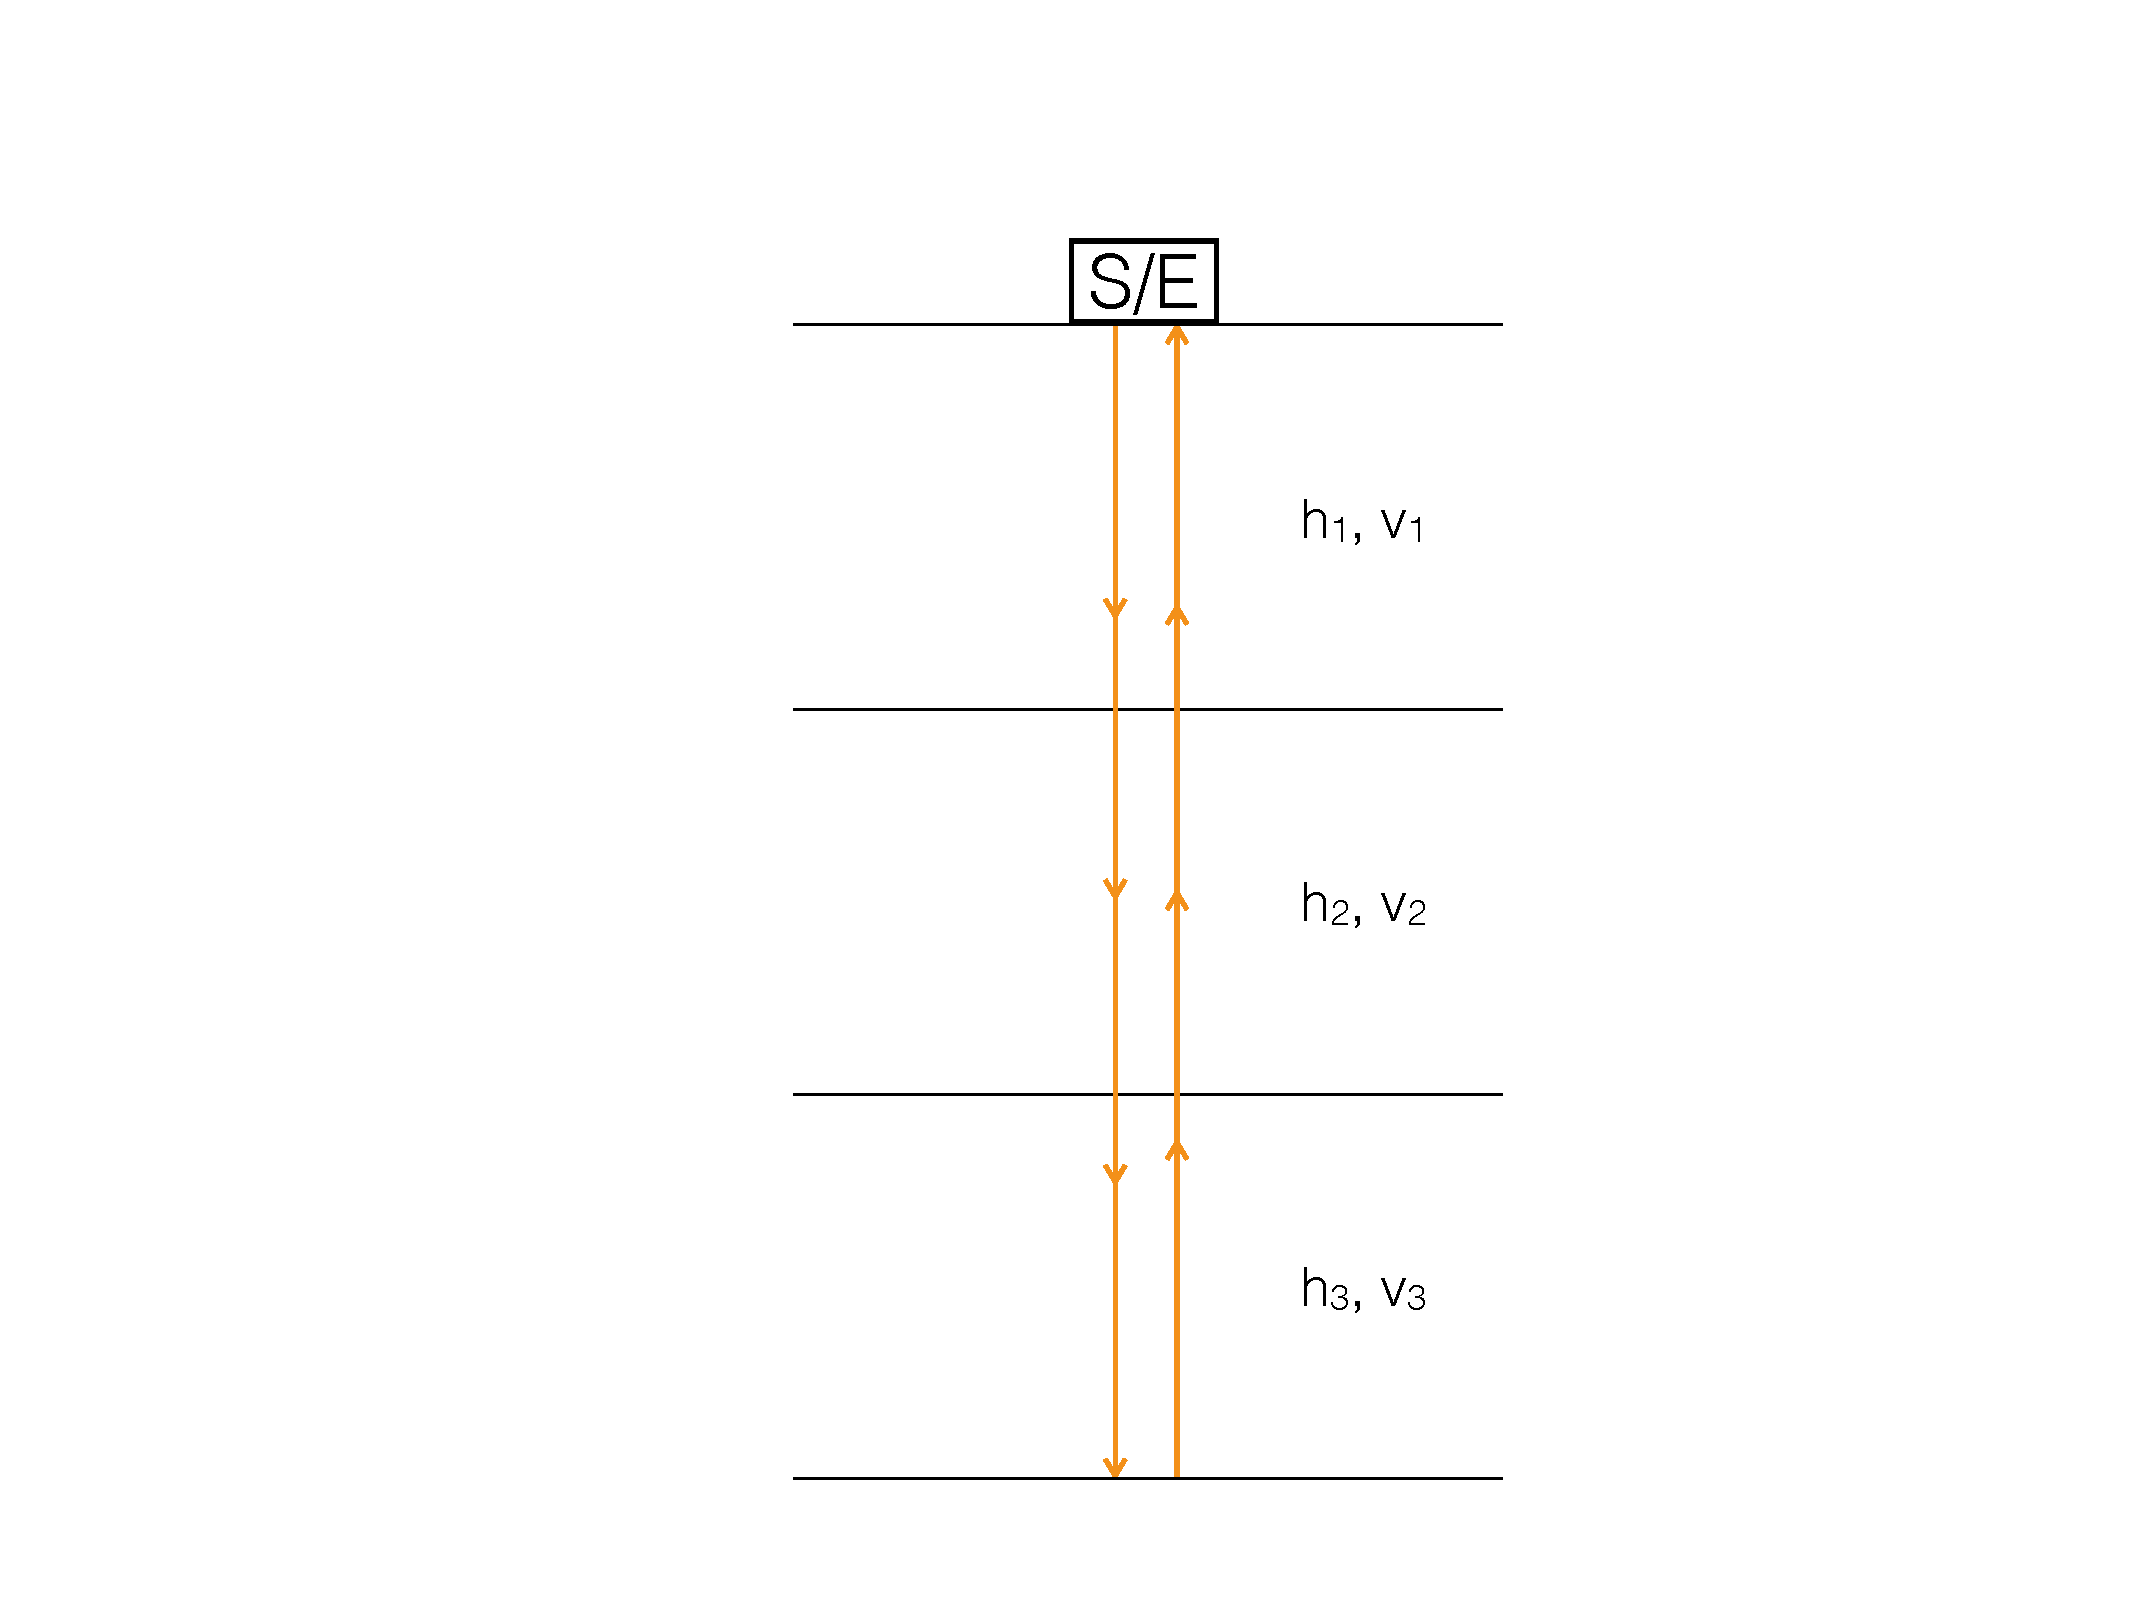
\includegraphics[scale = 0.3]{ReflexionsseismikBilder/ZeroOffset}
\end{figure}


Allerdings hat diese Methode einige \textbf{Probleme}: \begin{itemize}
	\item sehr anfällig für Verzerrungen: Laufzeiten entsprechen nicht Reflektortiefen
	\item schlechtes Signal-/Stör-Verhältnis: jeder Punkt im Untergrund wird nur einmal beleuchtet
	\item große Mehrdeutigkeiten
\end{itemize}

Durch Variation der Entfernung zwischen Sender und Empfänger, sowie einer Mehrfachabdeckung der Untergrundpunkte bei der Messung und Bestimmung des Geschwindigkeitsmodells, kann man diese Probleme lösen. Wie genau diese Messkonfiguration dann aussieht, und wie sie ausgewertet wird schauen wir uns im Folgenden an.

\section{Common-Midpoint-Technik}
Die Idee hinter dieser Methodik ist die Erweiterung eines Einzel-Offsets zu Multi-Offsets. Das bedeutet, dass wir alle Untergrundpunkte mehrfach durch Messungen abdecken. 

Unser Messaufbau sieht dann in etwa so aus: 

\begin{figure}[H]
	\centering
	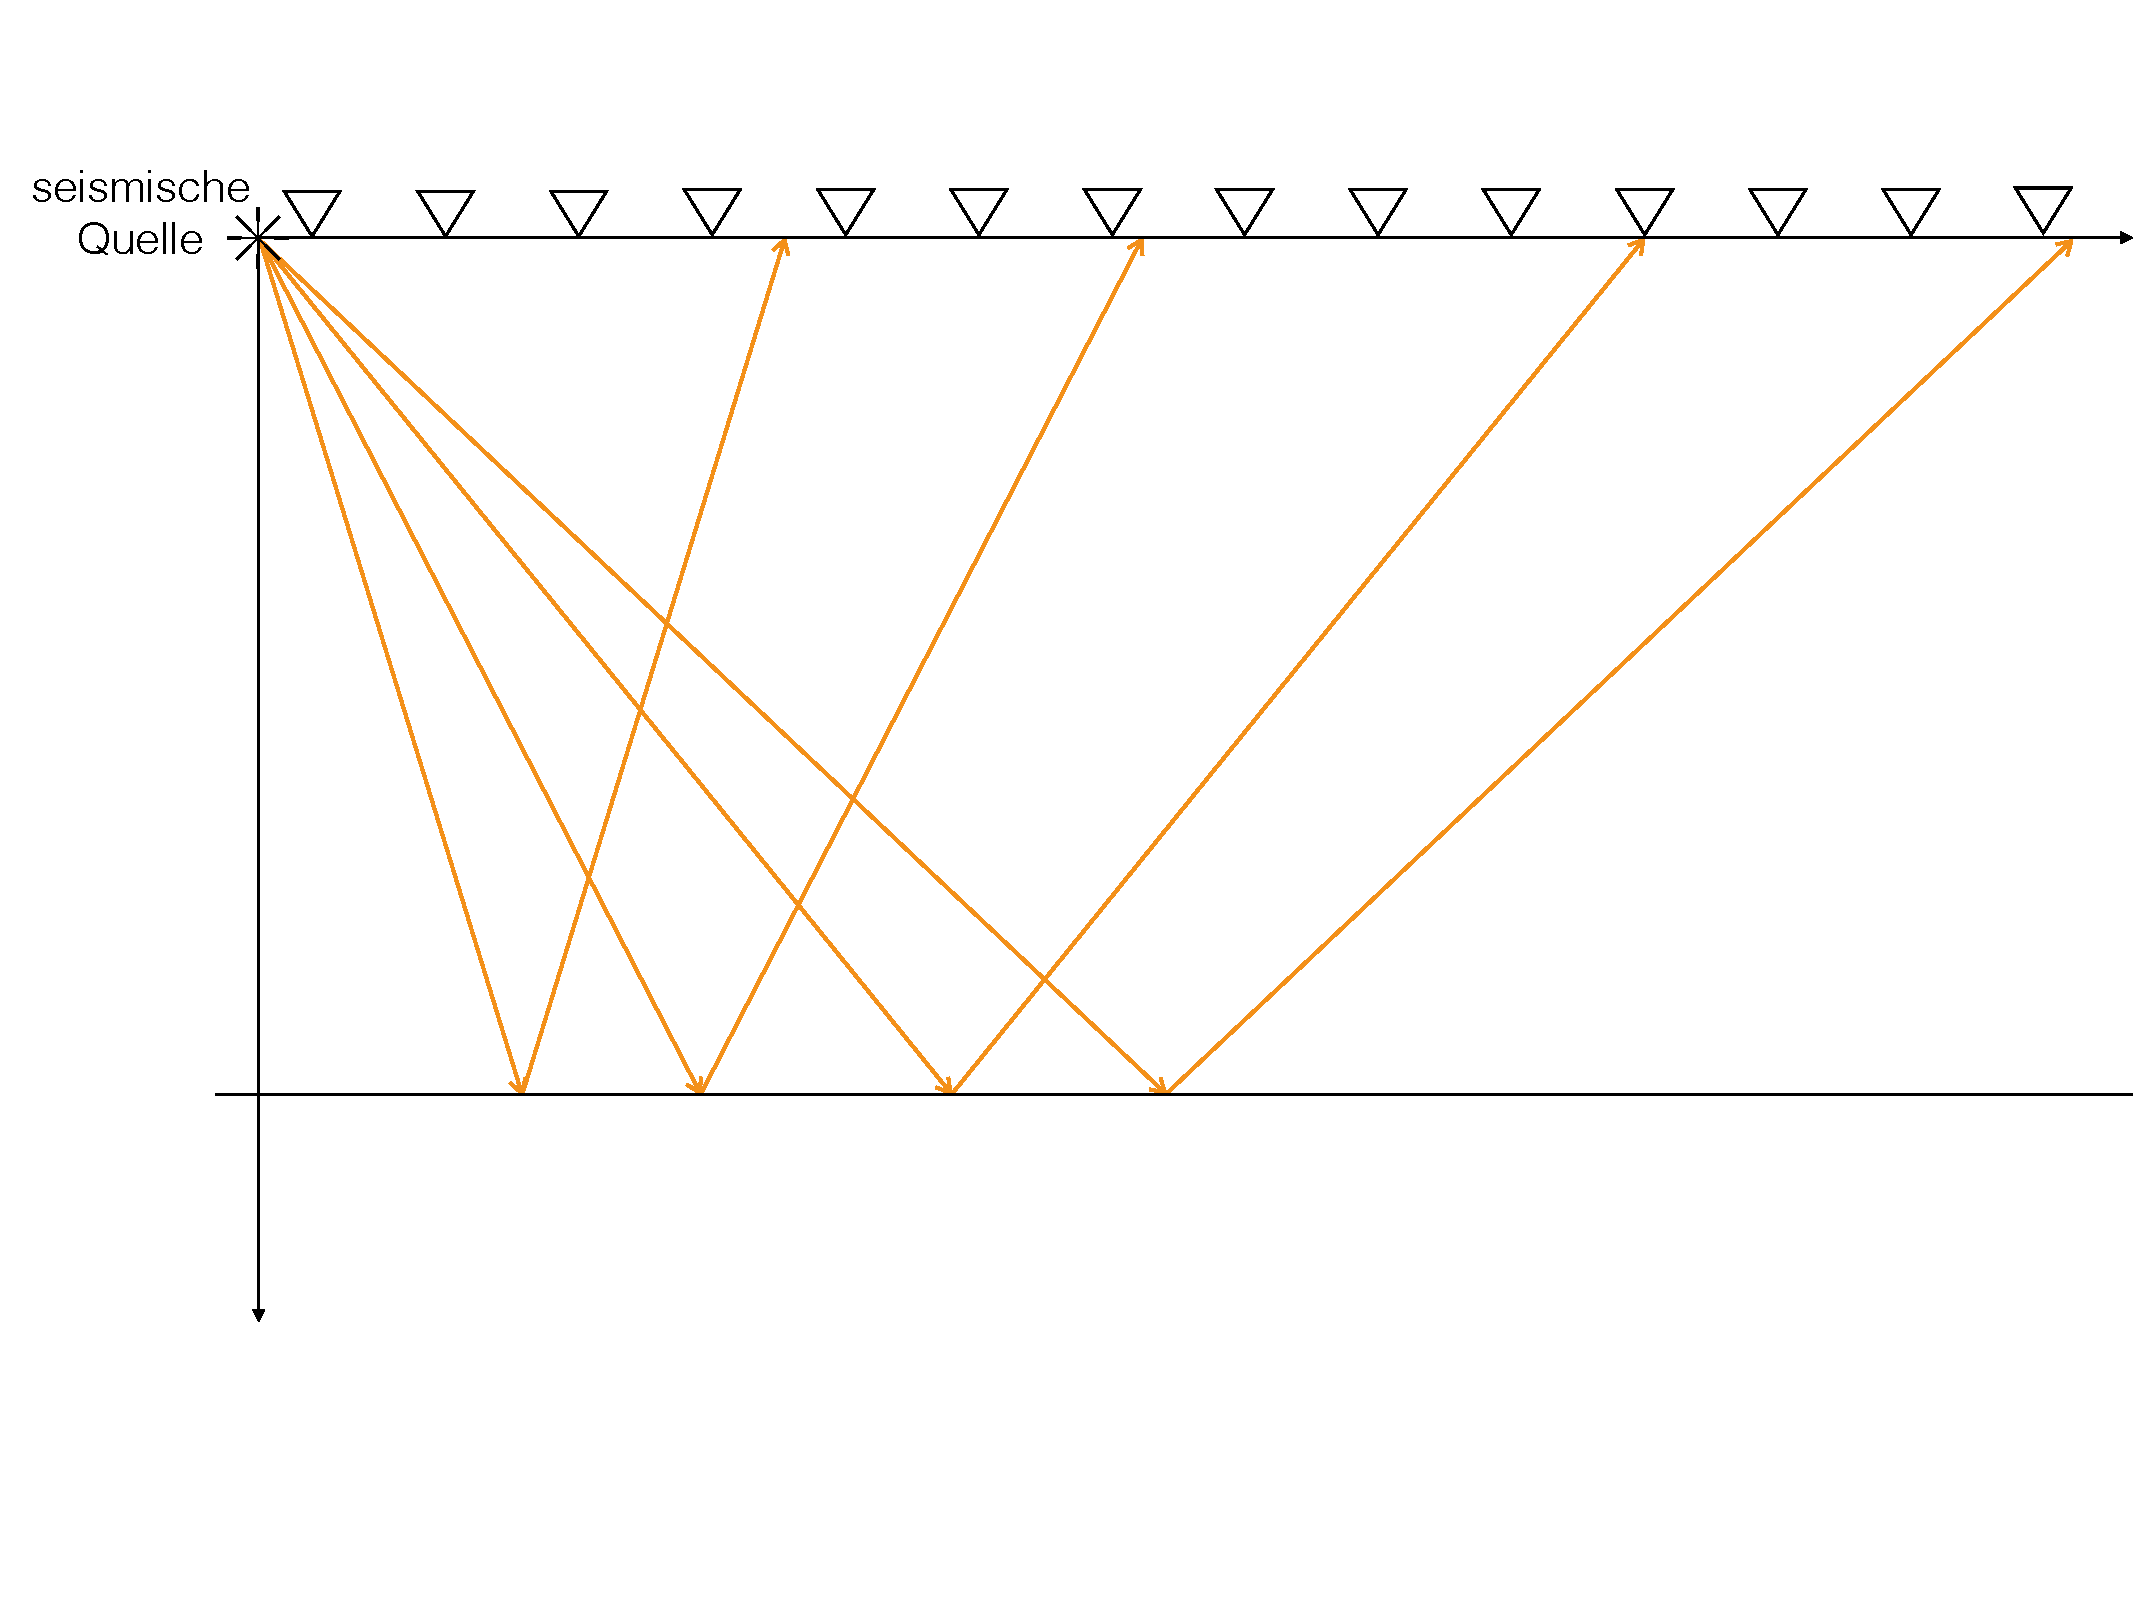
\includegraphics[width = \textwidth]{ReflexionsseismikBilder/MultiOffsetAnordnung}
\end{figure}


Im Wesentlichen besteht diese Messmethode aus fünf Arbeitsschritten: \begin{enumerate}[label={(\arabic*)}]
	\item Sortierung der Messpaare nach gemeinsamen Mittelpunkten (CMP)
	\item Geschwindigkeitsanalyse (Bestimmung von $v_{\text{nmo}}$)
	\item Laufzeitkorrektur
	\item Stapelung (Summation)
	\item Berechnung der Schichtgeschwindigkeiten
\end{enumerate}

Die einzelnen Arbeitsschritte werden im Folgenden erklärt.


\subsection{Sortierung nach CMP}
Der erste Schritt zur Auswertung ist die Sortierung der Messergebnisse nach einem gemeinsamen Mittelpunkt zwischen Quelle und Empfänger. Die so nach gemeinsamen Reflexionspunkt im Untergrund sortierten Seismogramme bilden einen \textbf{Common-Midpoint} (CMP). Liegt eine horizontale Schichtgrenze vor, liegt bei allen Messpaaren der Reflexionspunkt genau in der Mitte $x/2$ zwischen Sender und Empfänger (mit $x$ als Abstand Sender-Empfänger).

\begin{figure}[H]
	\centering
	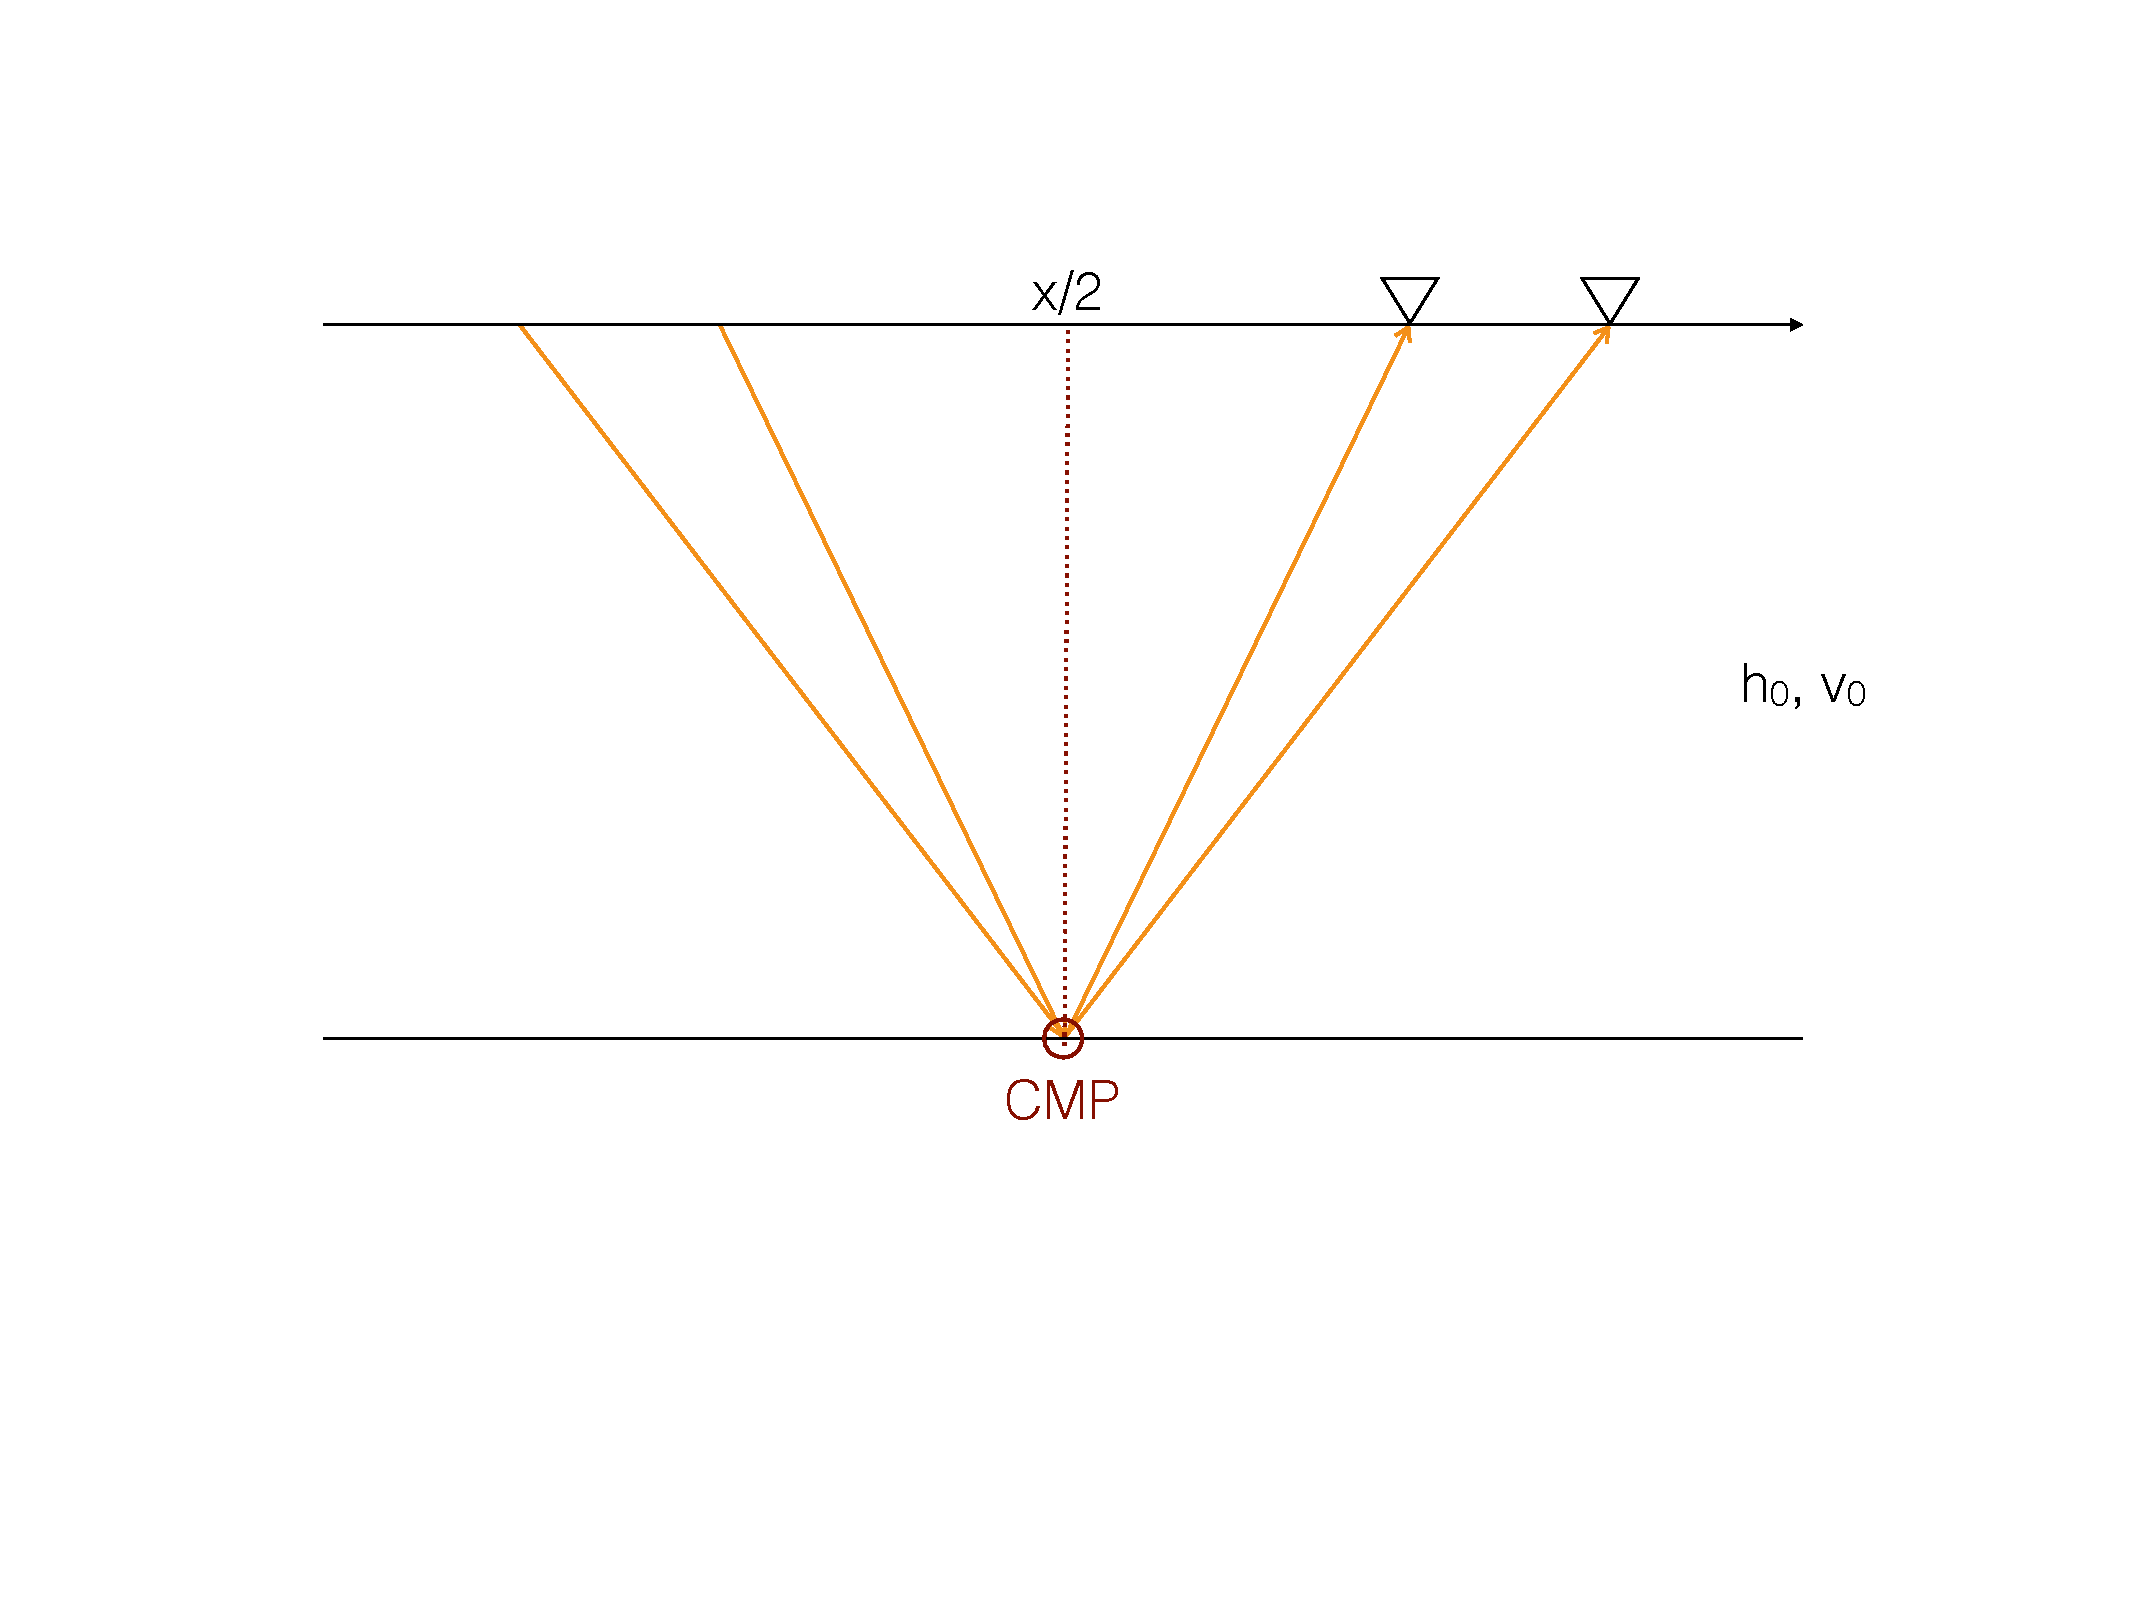
\includegraphics[width = \textwidth]{ReflexionsseismikBilder/CMPSortierung}
\end{figure}

\subsection{Laufzeitdiagramm und Geschwindigkeitsanalyse}
Wie auch schon bei der Refraktionsseismik interessieren wir uns besonders für die Ausbreitungsgeschwindigkeiten seismischer Wellen in allen Schichten. Um diese zu berechnen und zu analysieren, übertragen wir zunächst unsere gemessenen Werte in ein Laufzeitdiagramm. 

\begin{figure}[H]
	\centering
	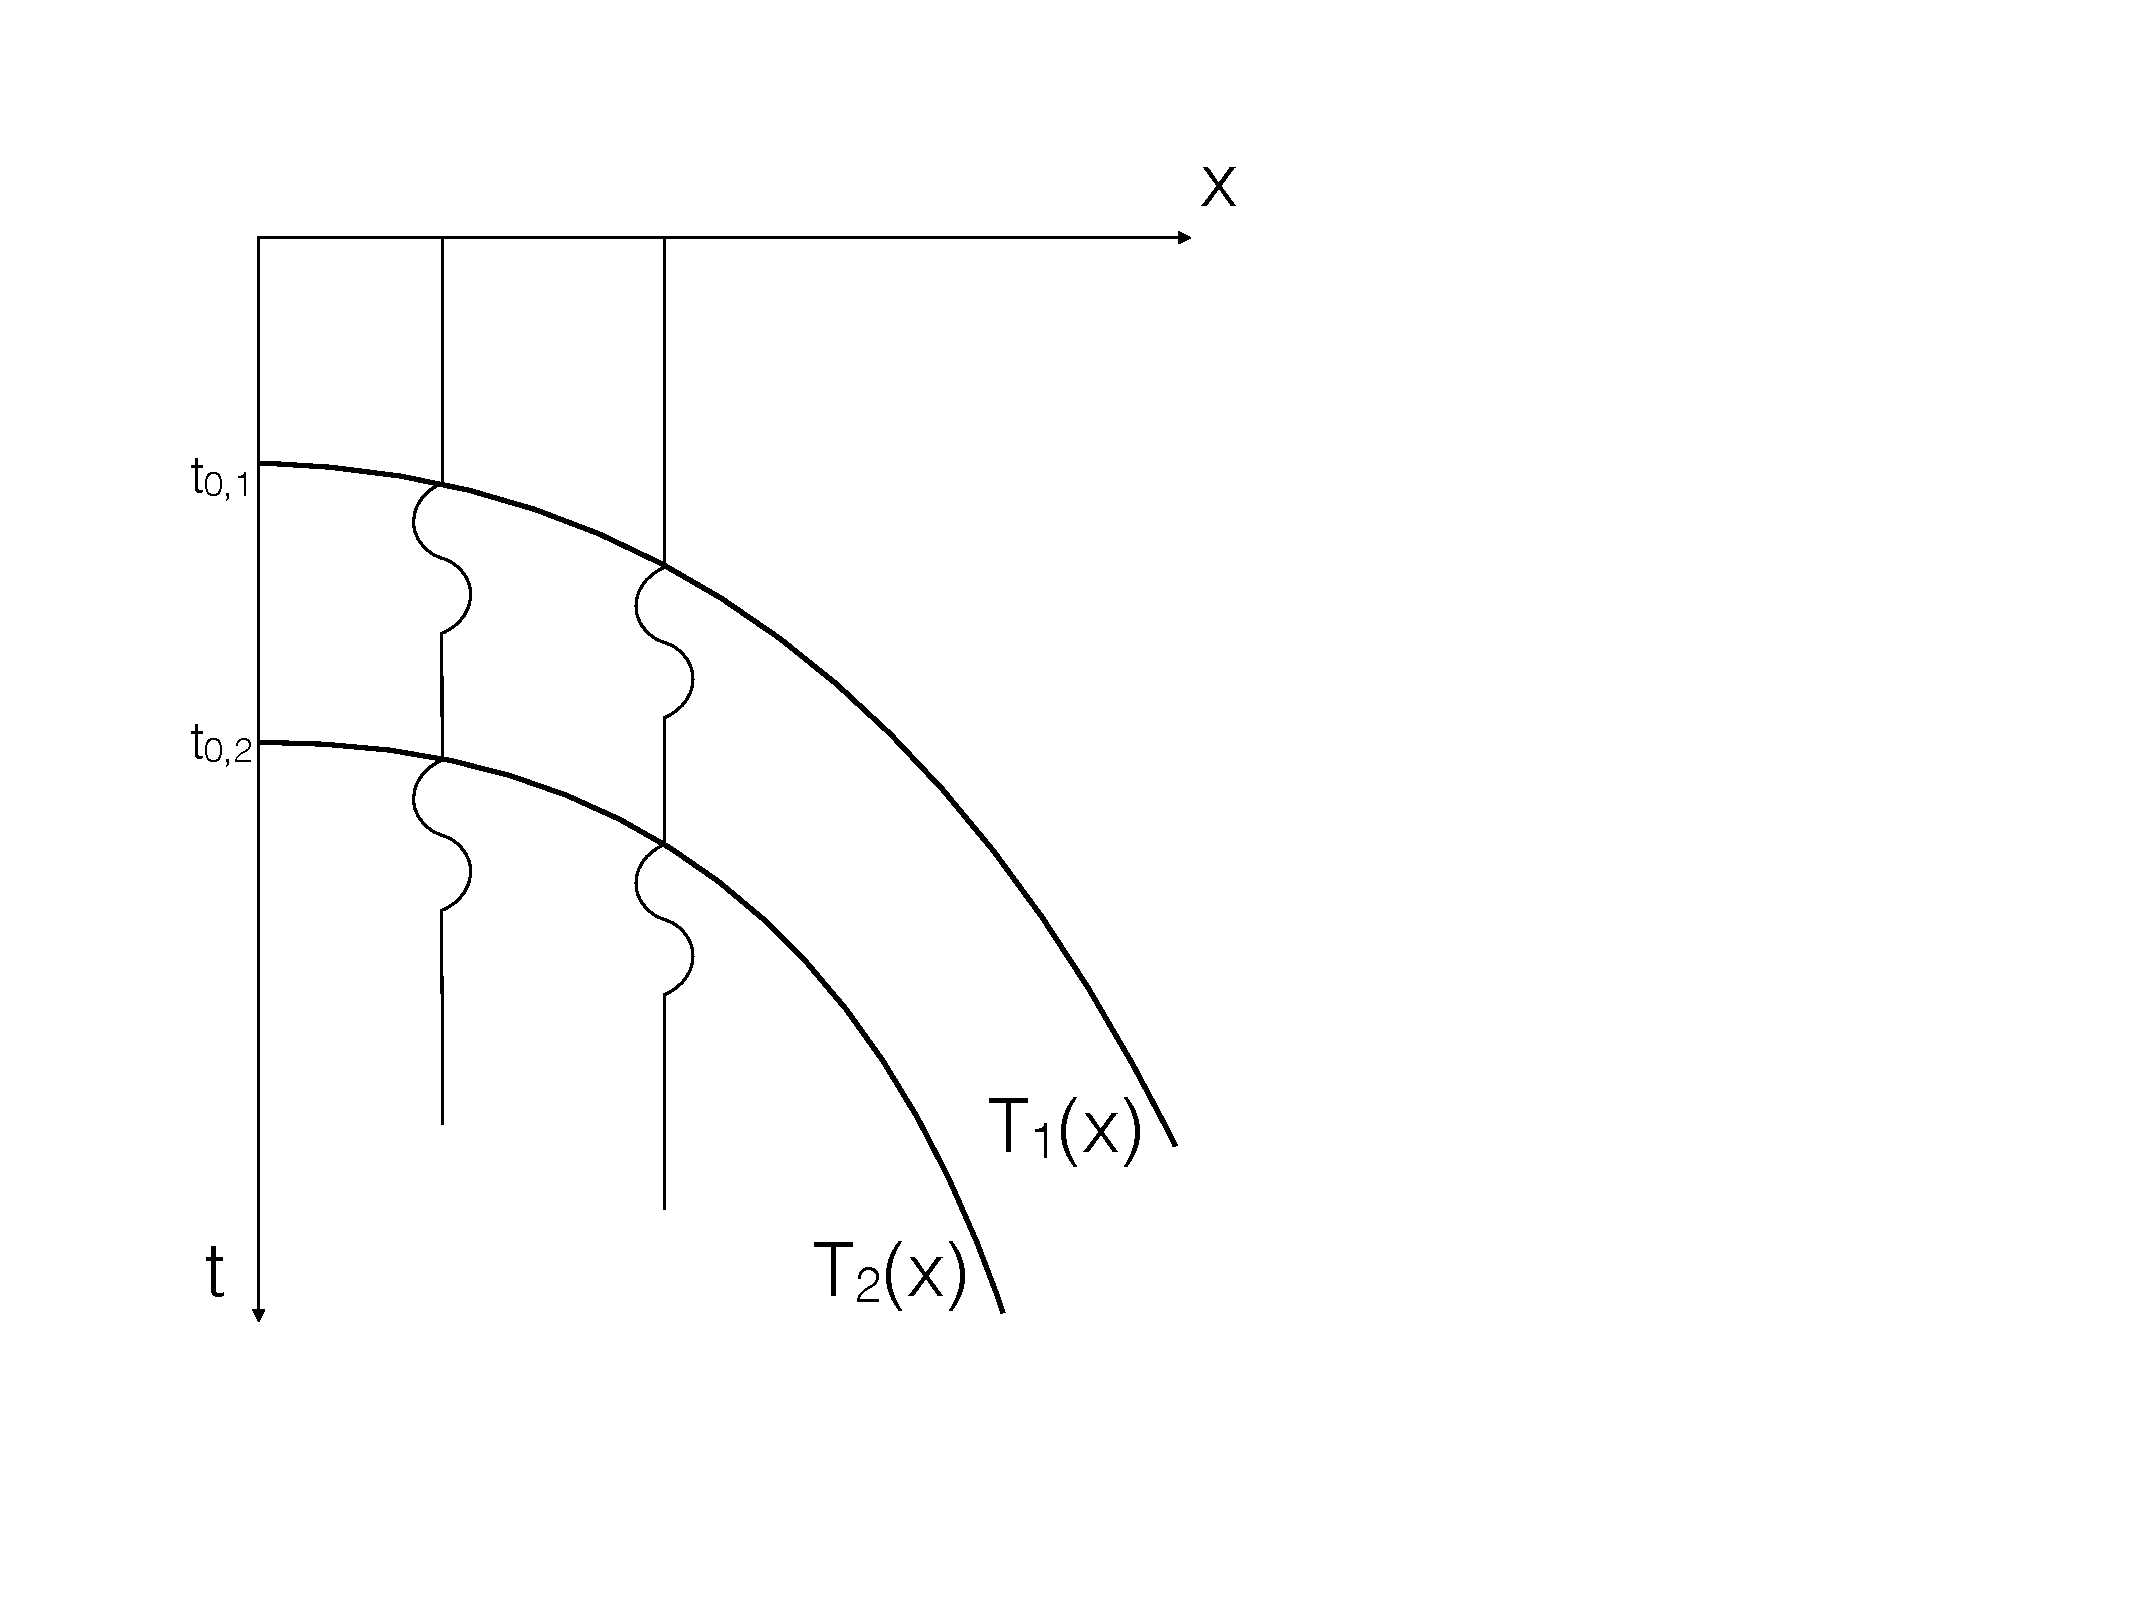
\includegraphics[scale = 0.3]{ReflexionsseismikBilder/t-x-Diagramm}
\end{figure} 


Die zugehörige Laufzeitgleichung ist nach Pythagoras: \begin{equation*}
	T^2(x) = \frac{x^2}{v_0^2} + t_0^2
\end{equation*}

Da diese Laufzeitgleichung eine Hyperbel ist, kann man die Geschwindigkeiten nicht einfach anhand der Steigung der Laufzeitkurve ablesen. Betrachtet man die Gleichung jedoch genauer, liegt nahe, die Messwerte in ein $T^2/ x^2$-Diagramm zu übertragen.

\begin{figure}[H]
	\centering
	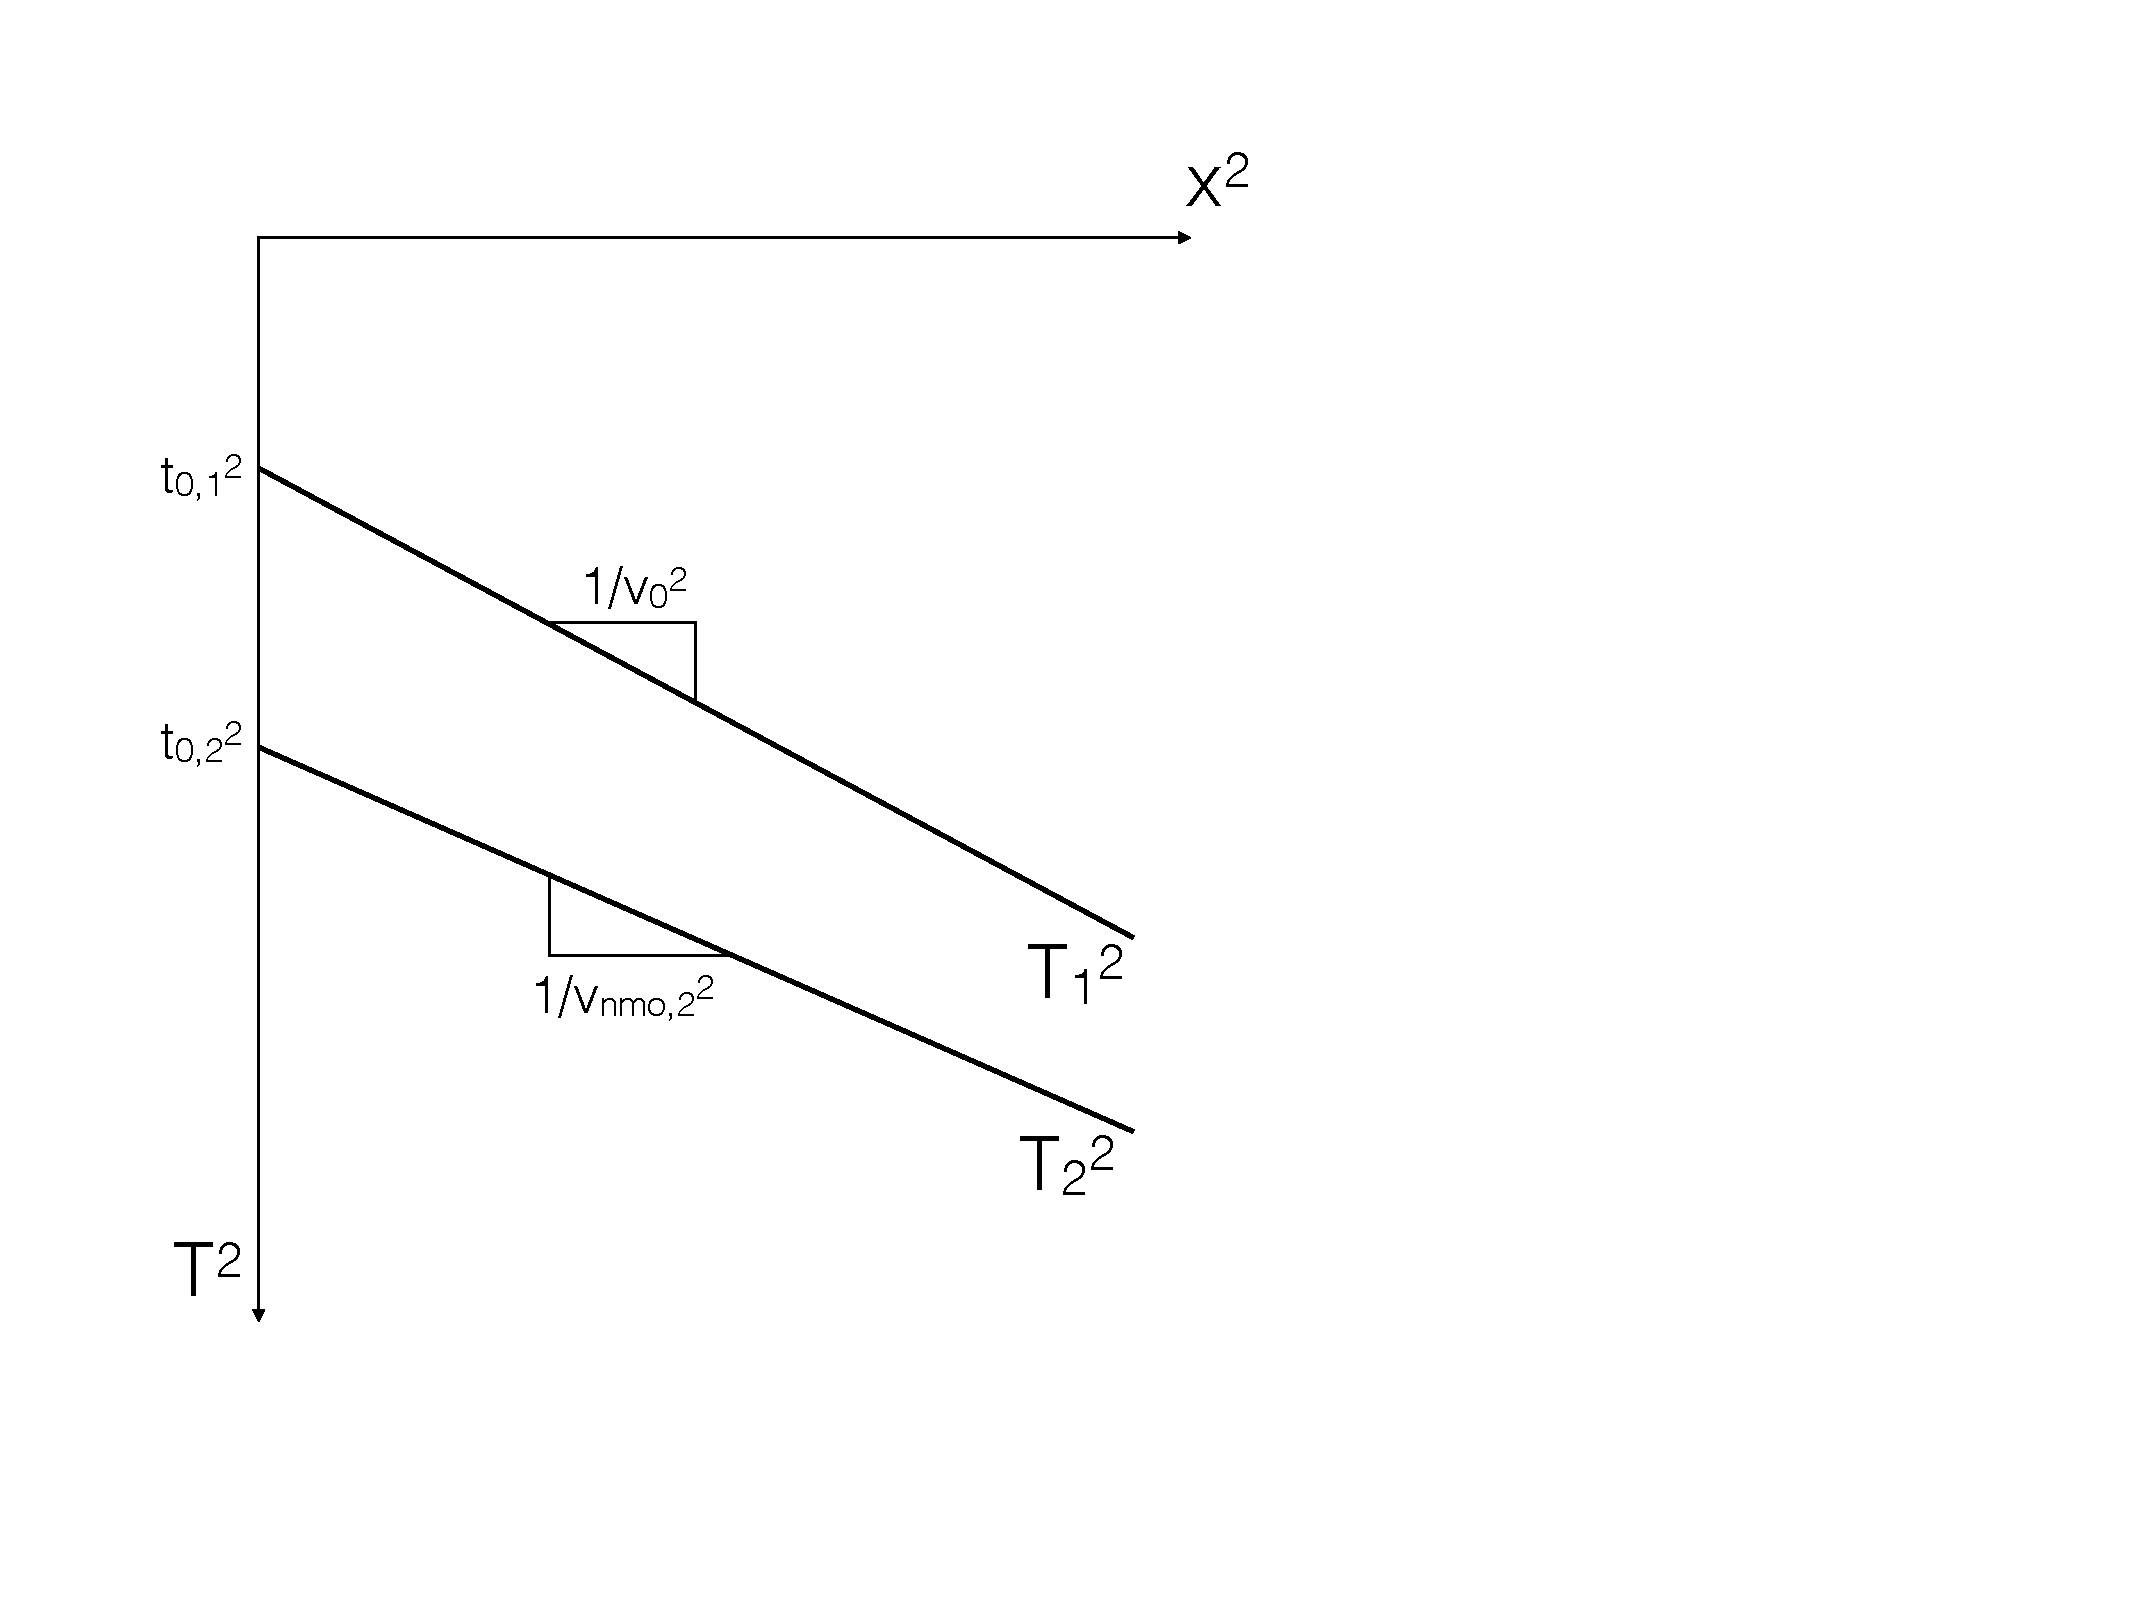
\includegraphics[scale = 0.3]{ReflexionsseismikBilder/T2-X2-Diagramm}
\end{figure}


An diesen Kurven könnte man nun die Geschwindigkeiten ablesen. Allerdings ist $T^2$ nur für die erste Schicht eine exakte Berechnung. Für alle weiteren ist sie nur eine Näherung. Die Geschwindigkeit, die man nach Berechnung der Steigung erhält, ist die \textbf{Normal-Moveout-Geschwindigkeit} $v_{\text{nmo}}$. Diese gibt lediglich die durchschnittliche Geschwindigkeit über alle Schichten an. \begin{align*}
	T_1^2(x) &= \frac{x^2}{v_1^2} + t_{0,1}^2 \\
	T_2^2(x) &\approx \frac{x^2}{v_{\text{nmo},2}^2} + t_{0,2}^2
\end{align*}

\subsection{Laufzeitkorrektur}
Das Ziel der CMP-Methode ist die Simulation einer Zero-Offset-Anordnung mit eindeutigen Ergebnissen durch mehrfache Abdeckung eines Untergrundpunktes. 

\begin{figure}[H]
	\centering
	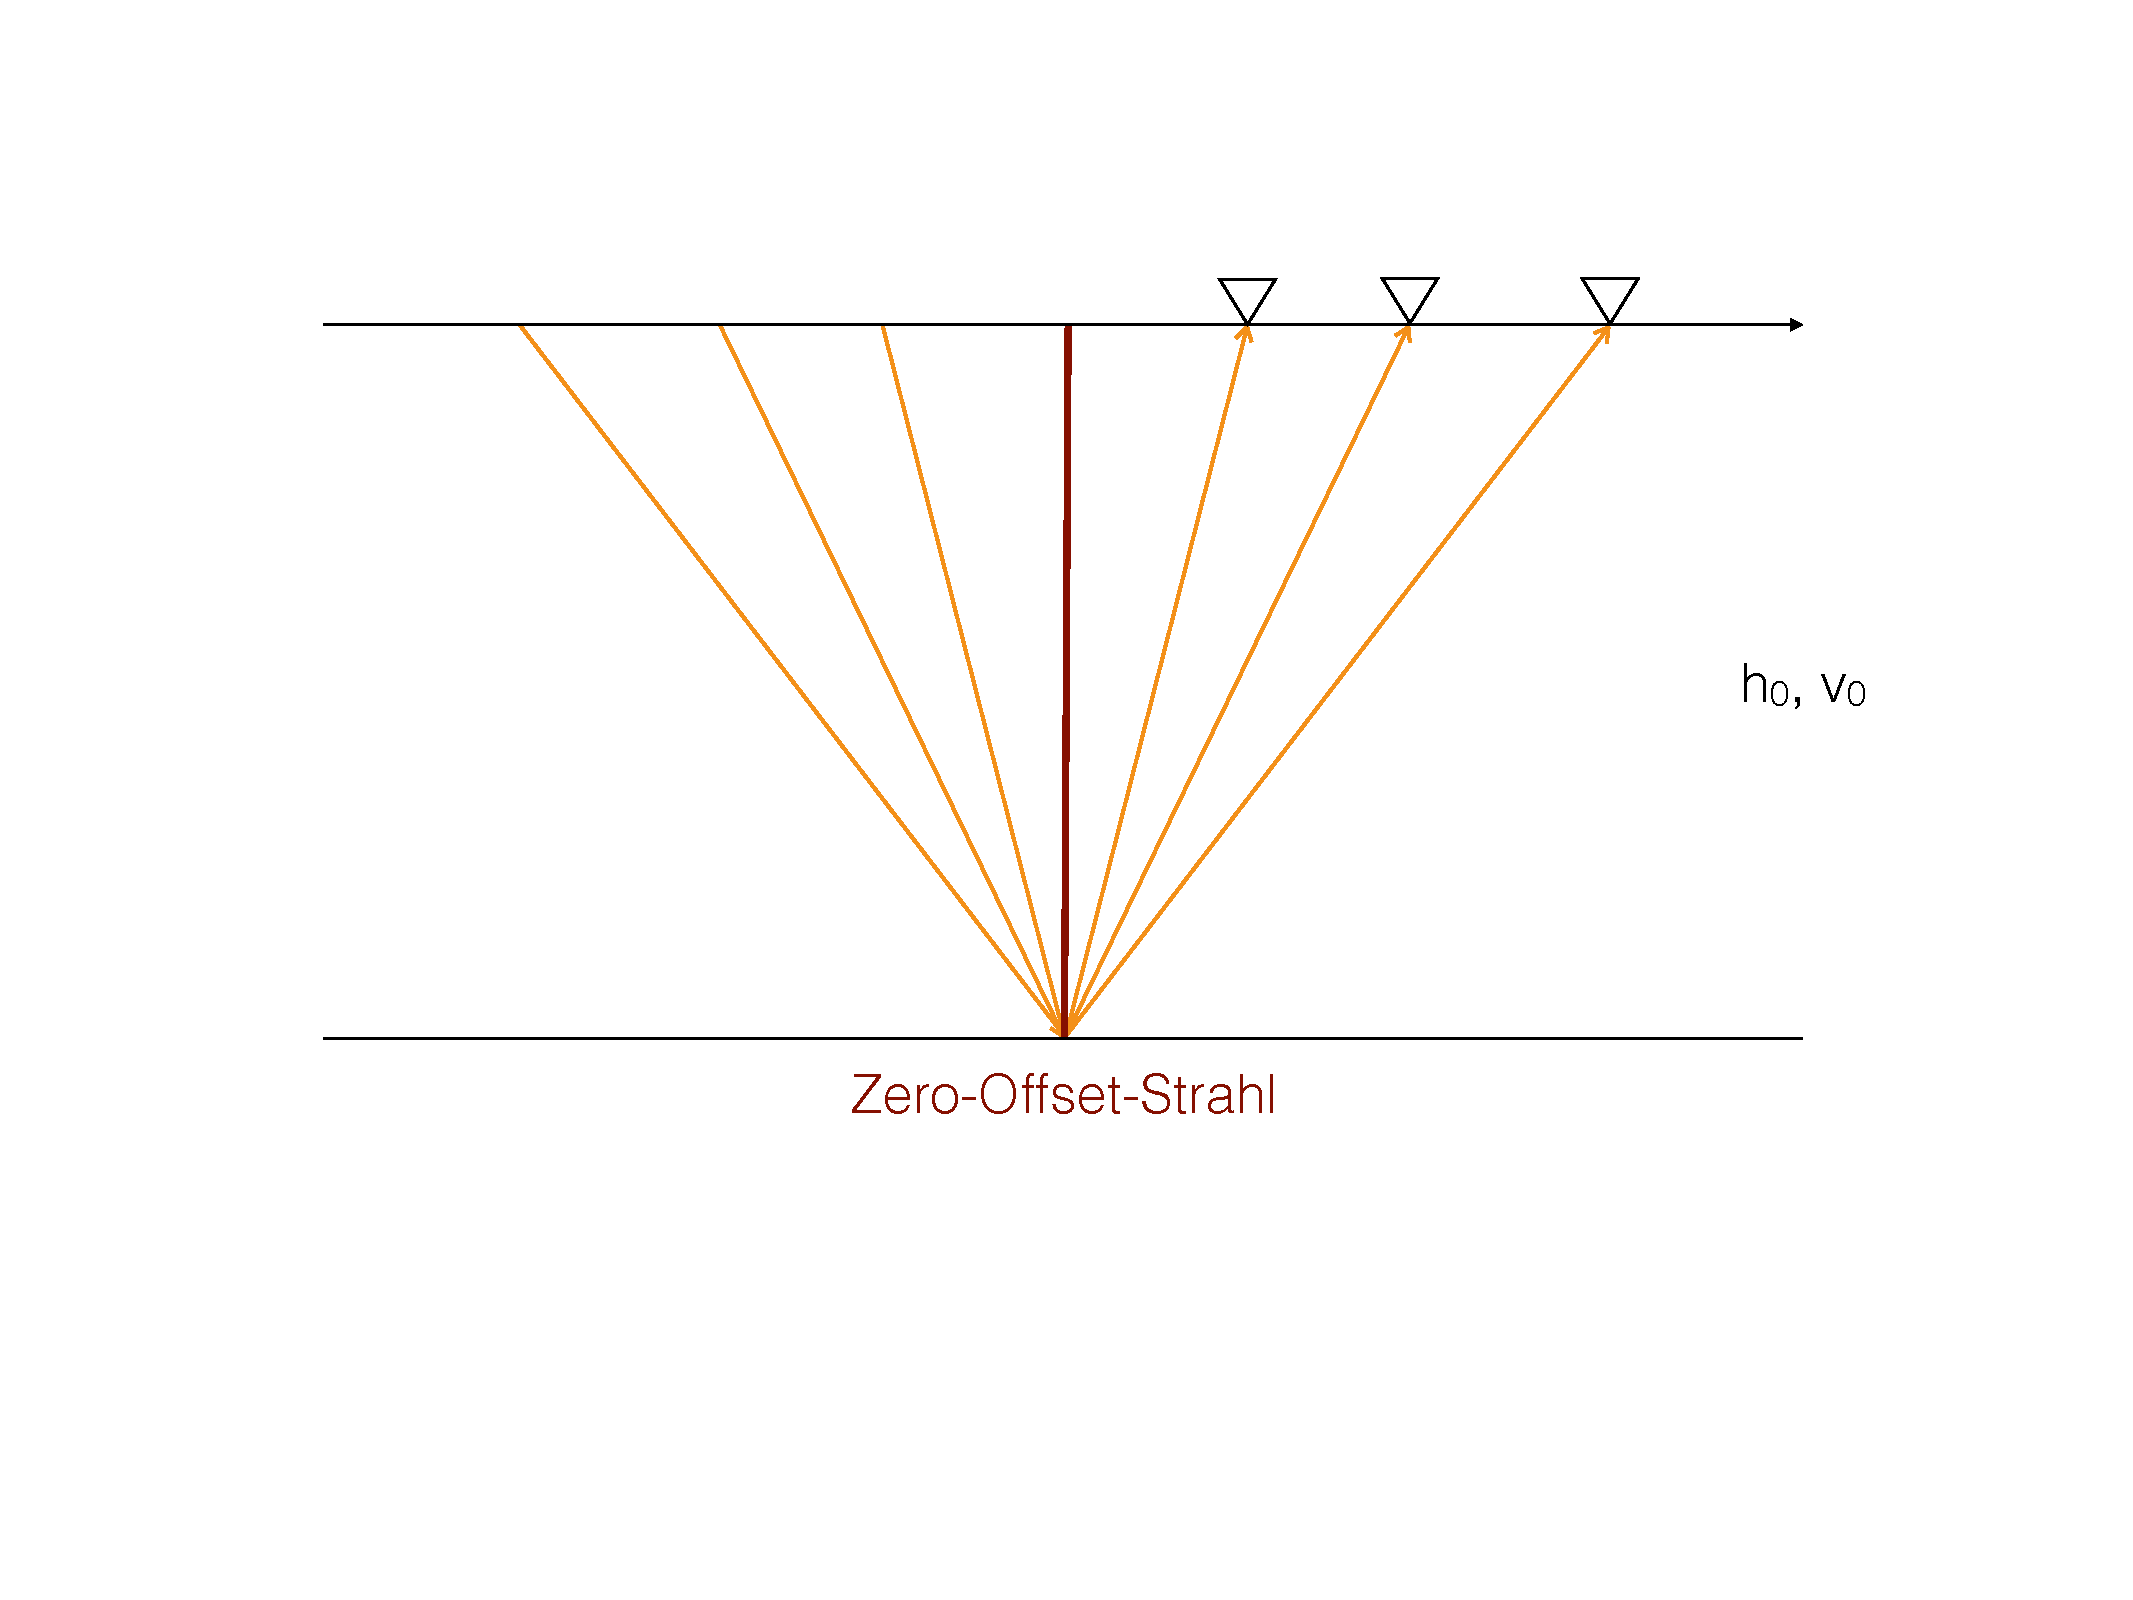
\includegraphics[width = \textwidth]{ReflexionsseismikBilder/ZeroOffsetStrahl}
\end{figure}

Betrachten wir erneut die Messauslage nach CMP-Sortierung und die zugehörige Laufzeitkurve: 

\begin{figure}[H]
	\begin{subfigure}[m]{0.5\textwidth}
	\centering
		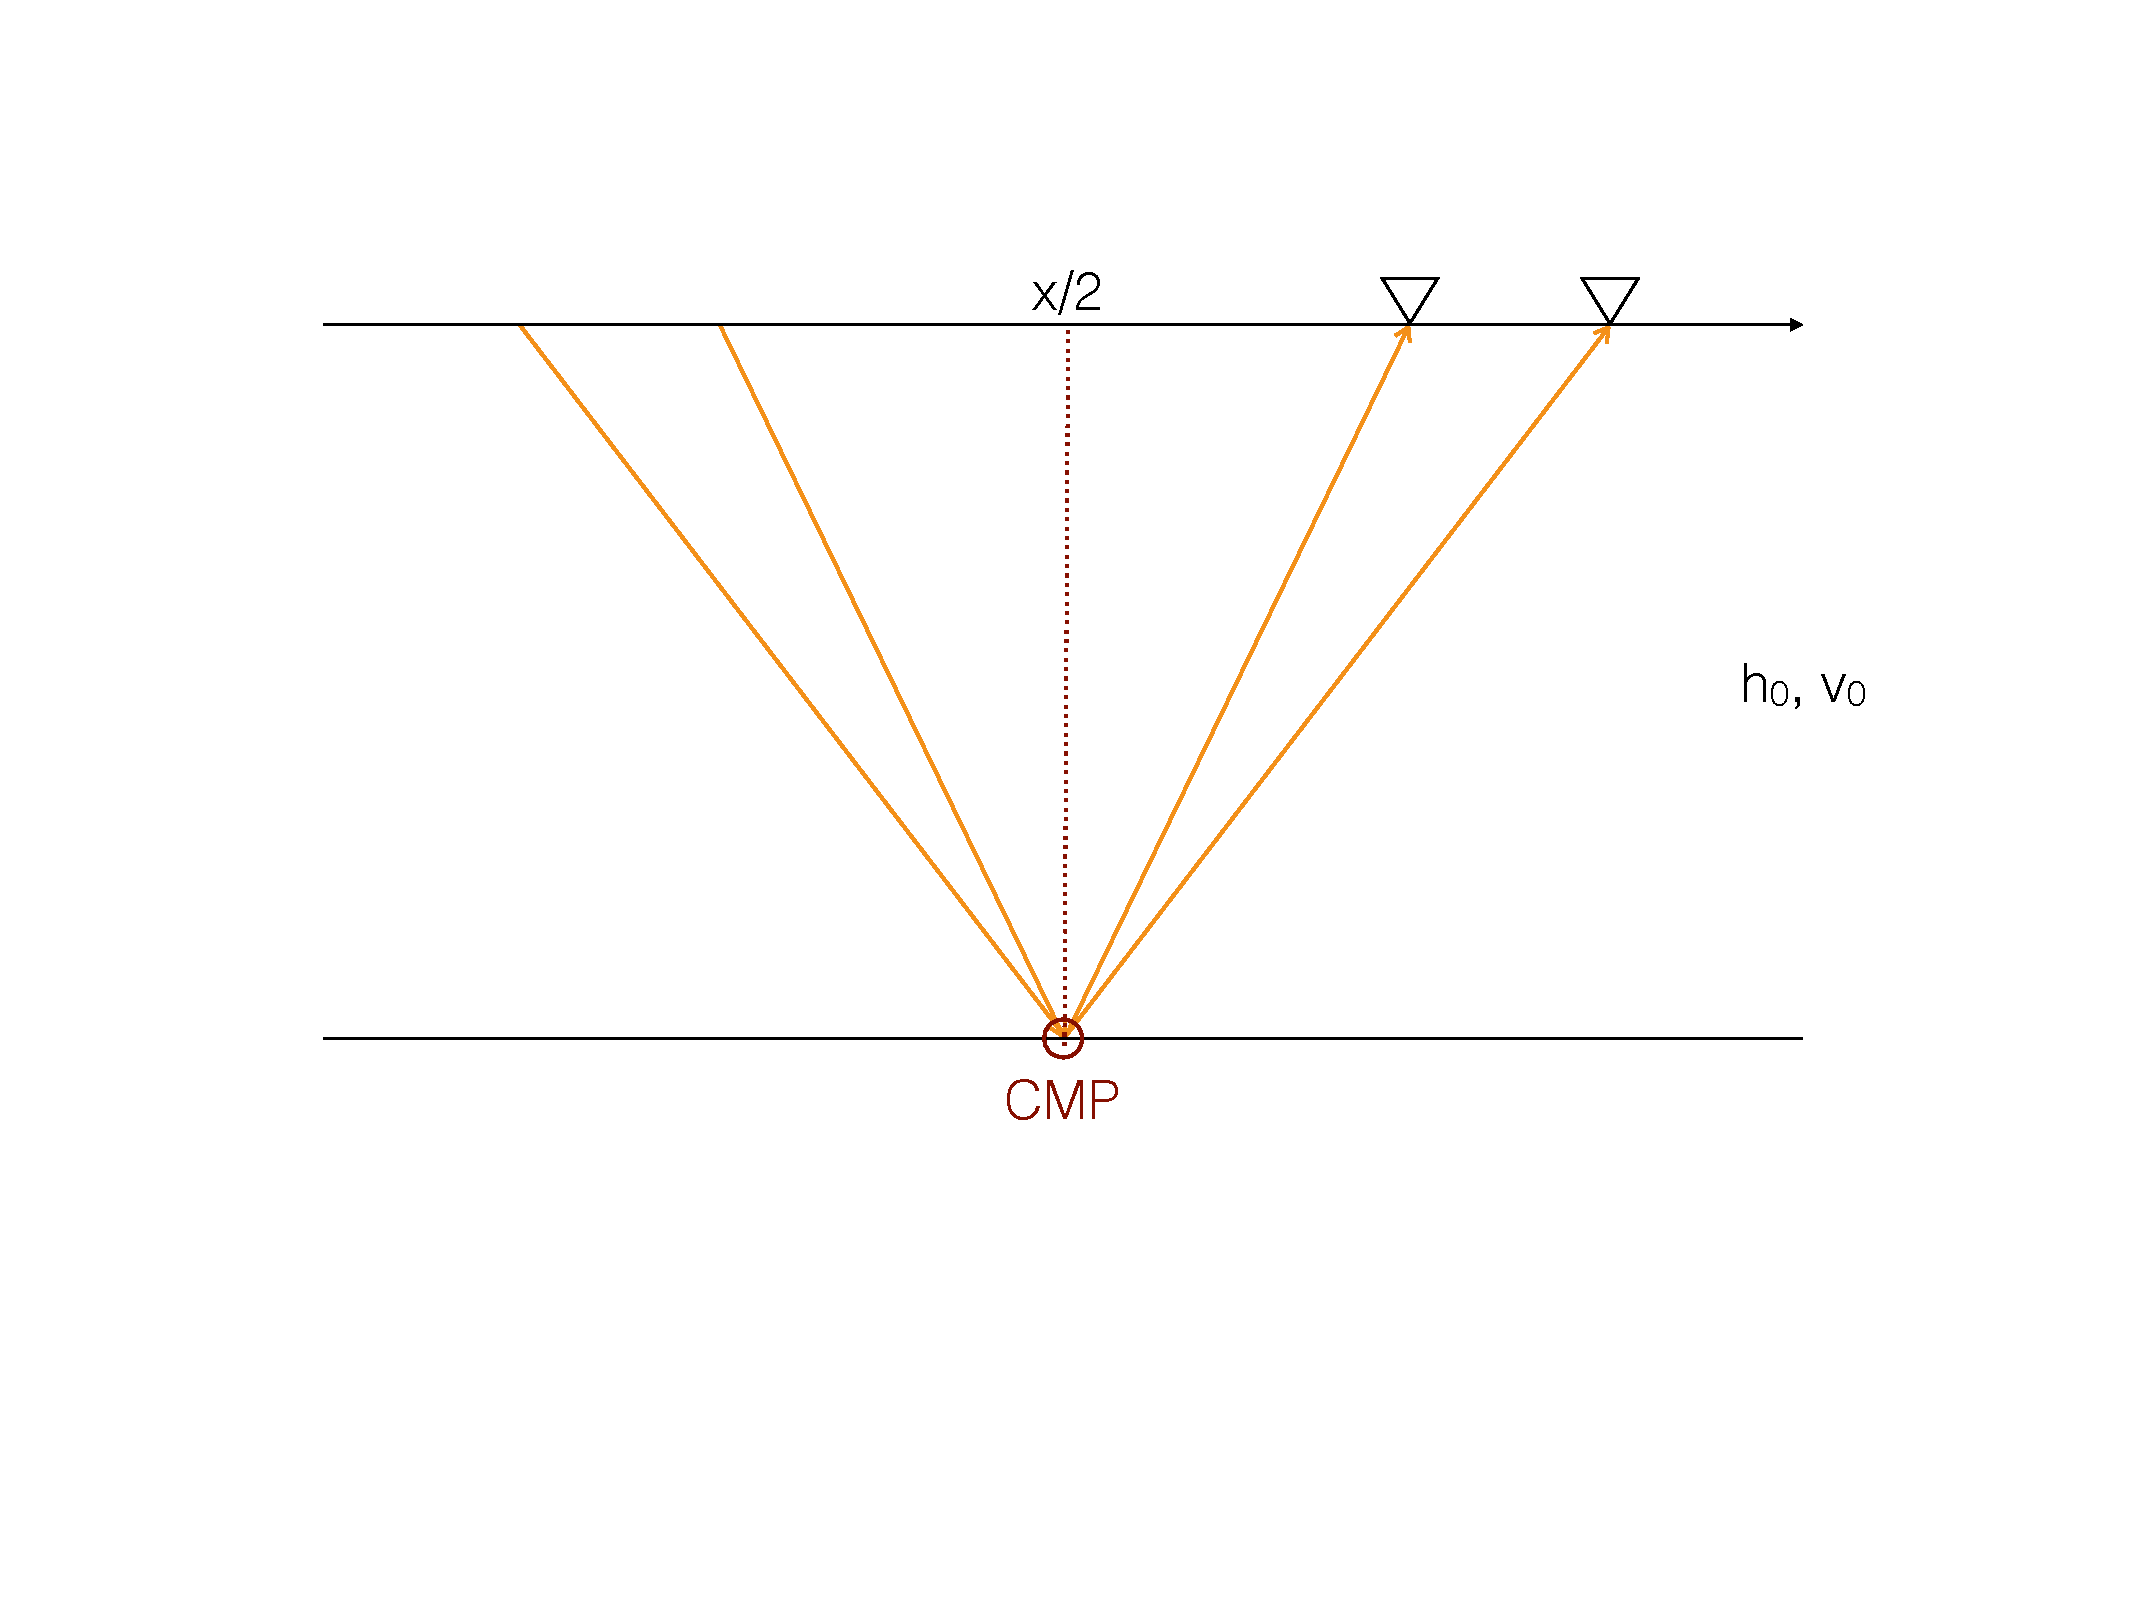
\includegraphics[scale = 0.2]{ReflexionsseismikBilder/CMPSortierung}	
	\end{subfigure}
	\begin{subfigure}[m]{0.5\textwidth}
	\centering
		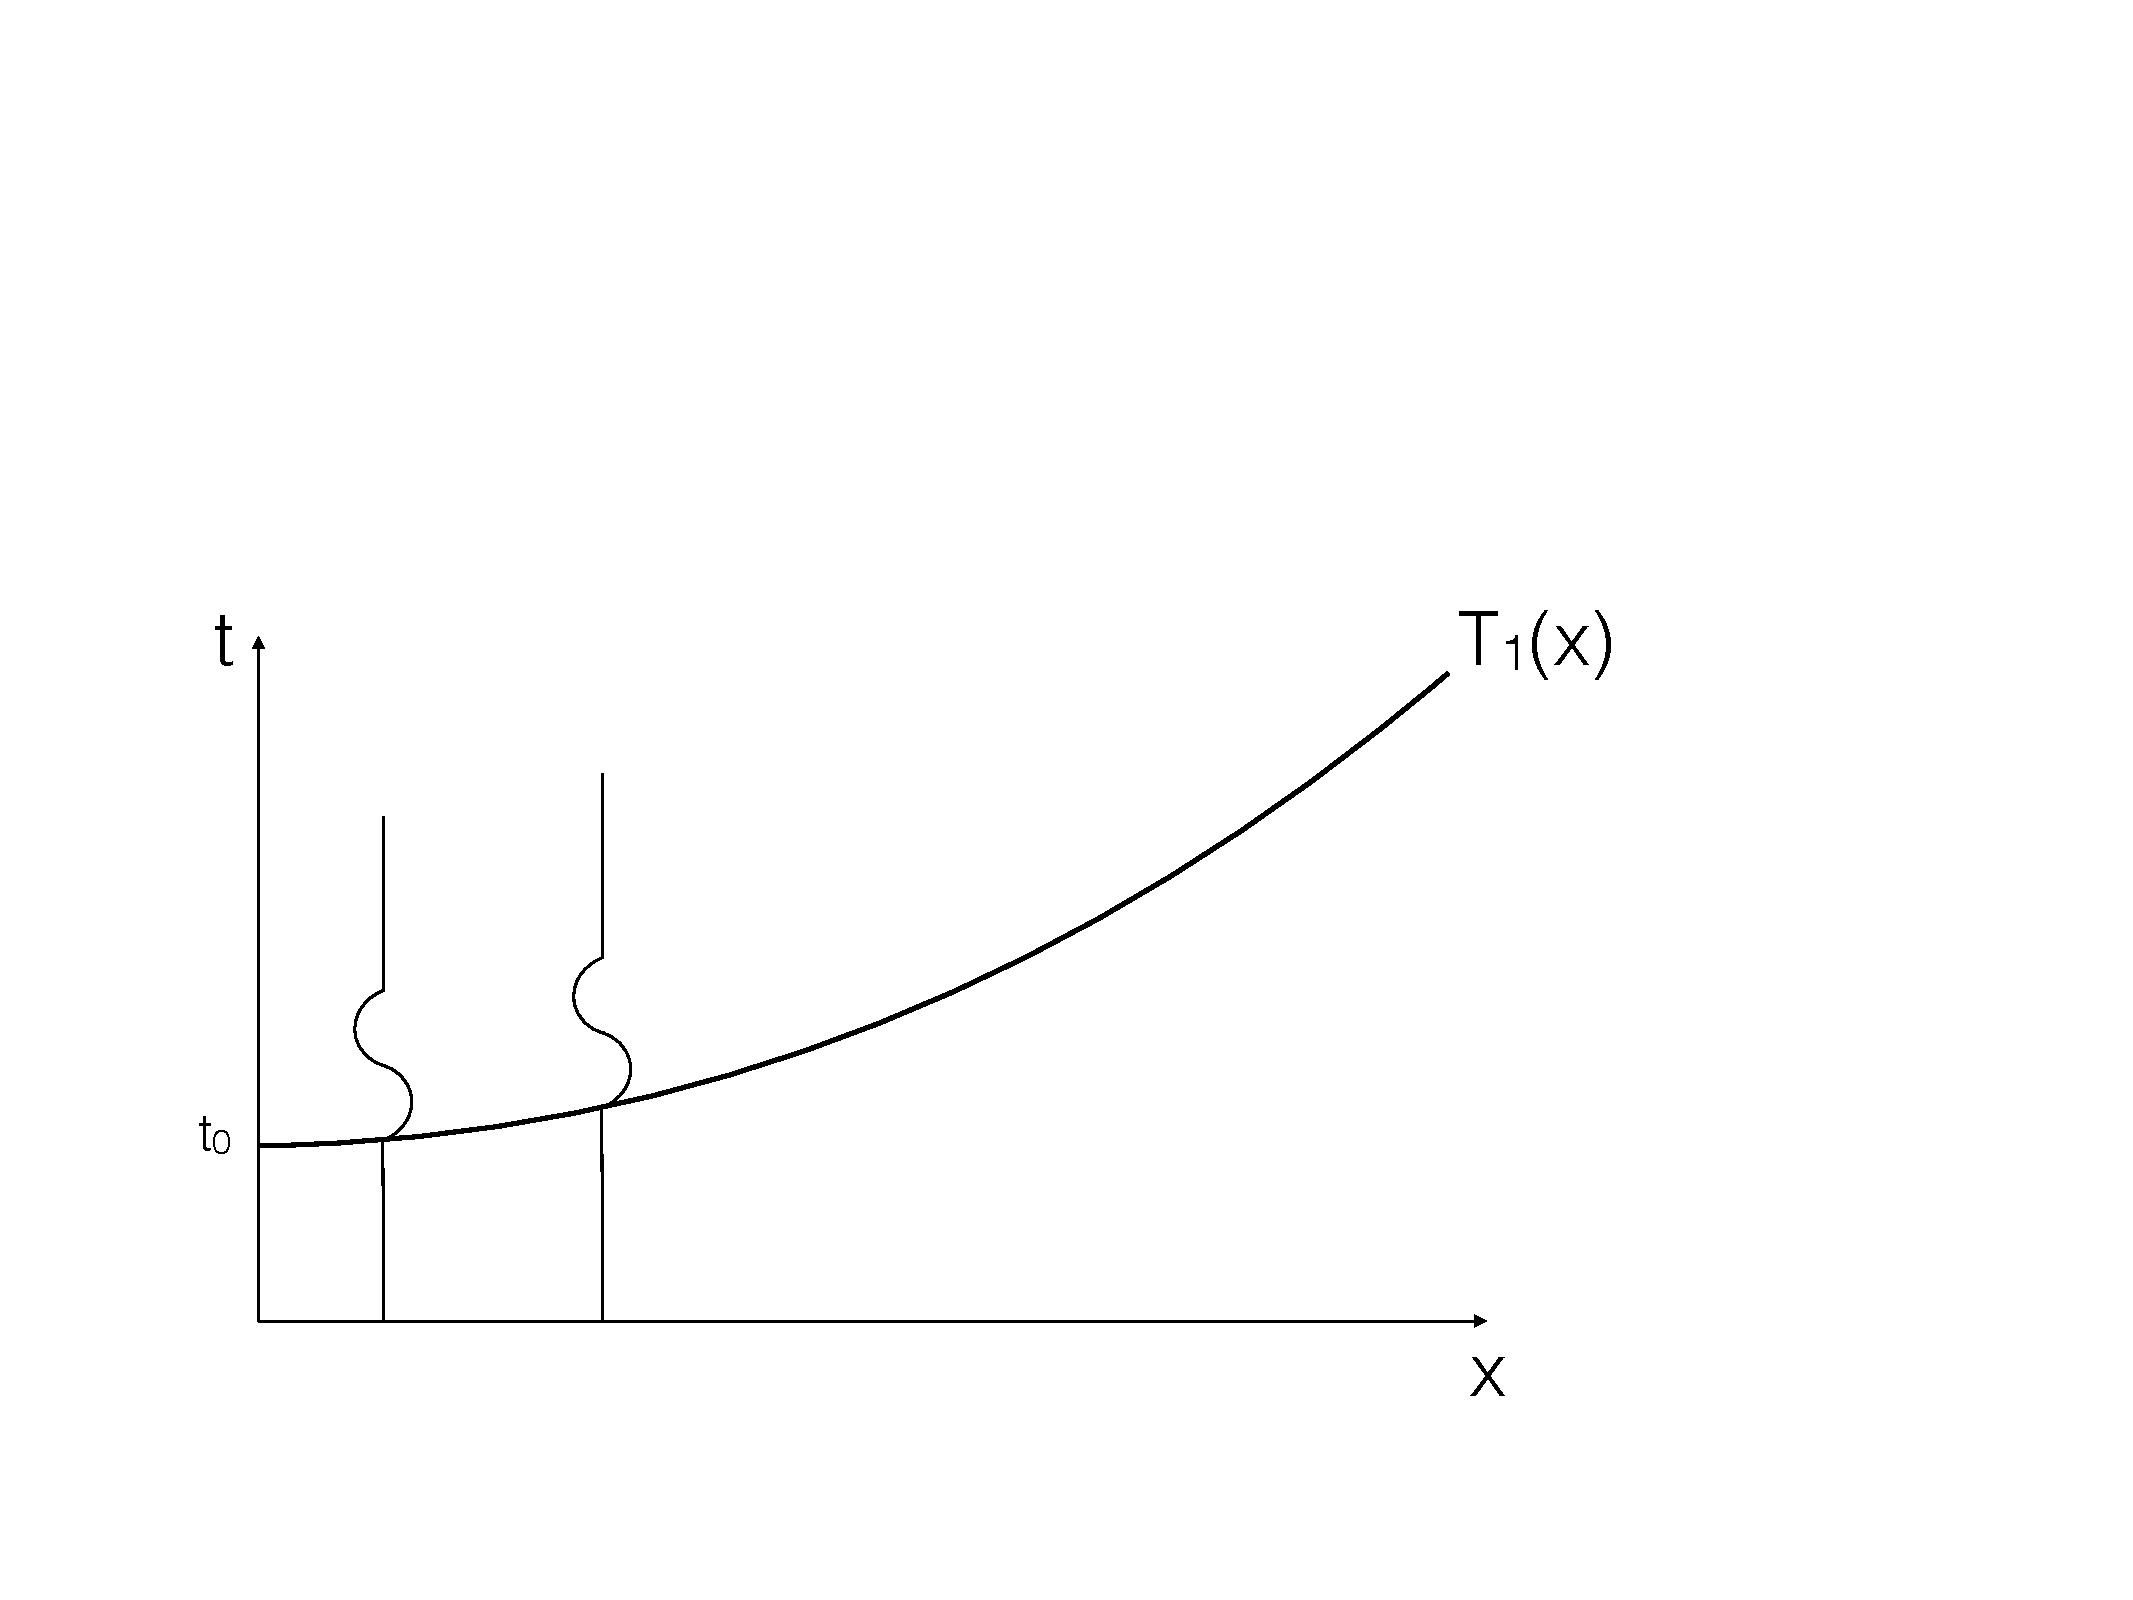
\includegraphics[scale = 0.2]{ReflexionsseismikBilder/LaufzeitCMP}
	\end{subfigure}
\end{figure}


Die Laufzeit der Welle mit dem kürzesten Weg ist genau $t_0$. Dieser Weg entspricht dem eines Zero-Offset-Strahls, also senkrecht nach unten und wieder nach oben.
Da die Wellen bei allen anderen Messauslagen einen größeren Weg zurücklegen müssen, ist die Laufzeitkurve eine Hyperbel und keine Gerade. Eine solche wollen wir aber erzeugen. Aus diesem Grund ist eine Laufzeitkorrektur durchzuführen. Diese Korrektur gleicht die längere Laufzeit, verursacht durch längere Strahlenwege, aus. 


\begin{equation*}
	\Delta t_{\text{nmo}} = T_1(x) - t_0 = \sqrt{\frac{x^2}{v_{\text{nmo}}^2} + t_0^2} - t_0
\end{equation*}   

\begin{figure}[H]
	\centering
	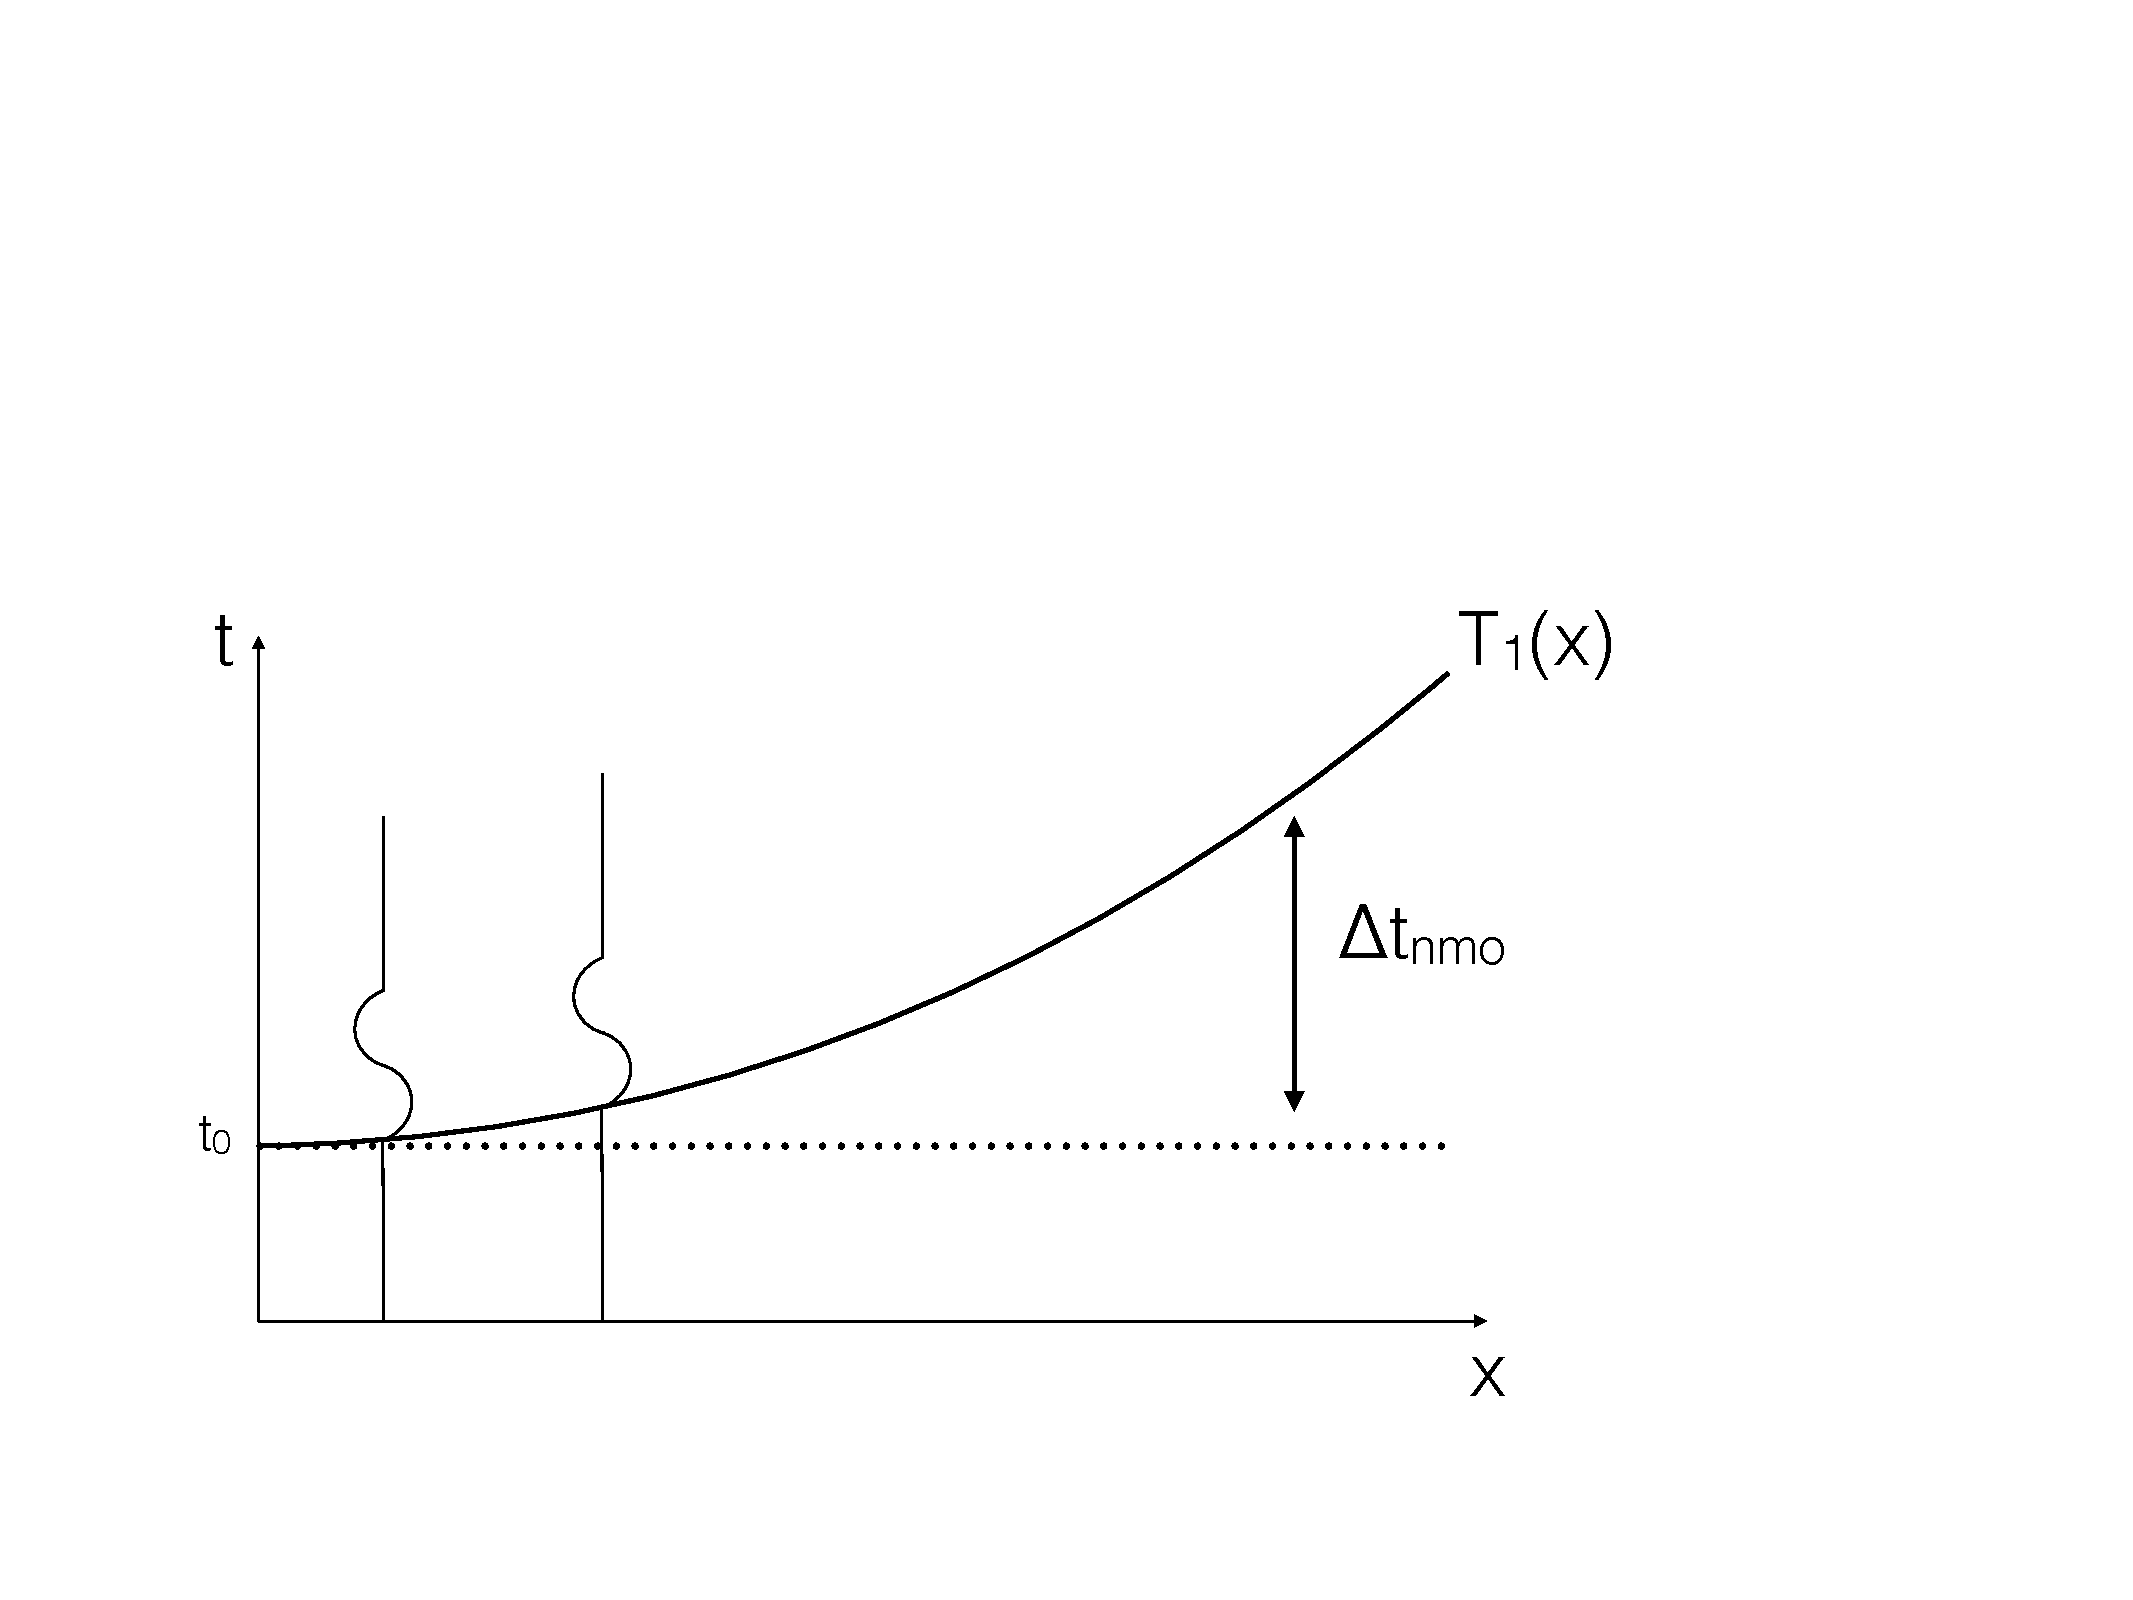
\includegraphics[scale = 0.3]{ReflexionsseismikBilder/tnmoAnpassung}
\end{figure}

\subsection{Stapelung}
Nachdem wir alle Messwerte auf eine Zeit normiert haben, werden die Seismogrammdaten gestapelt, das heißt aus allen Seismogrammen wird ein einziges pro CMP. Das Ergebnis ist ein Zero-Offset-Strahl ohne Mehrdeutigkeiten.

\begin{figure}[H]
	\centering
	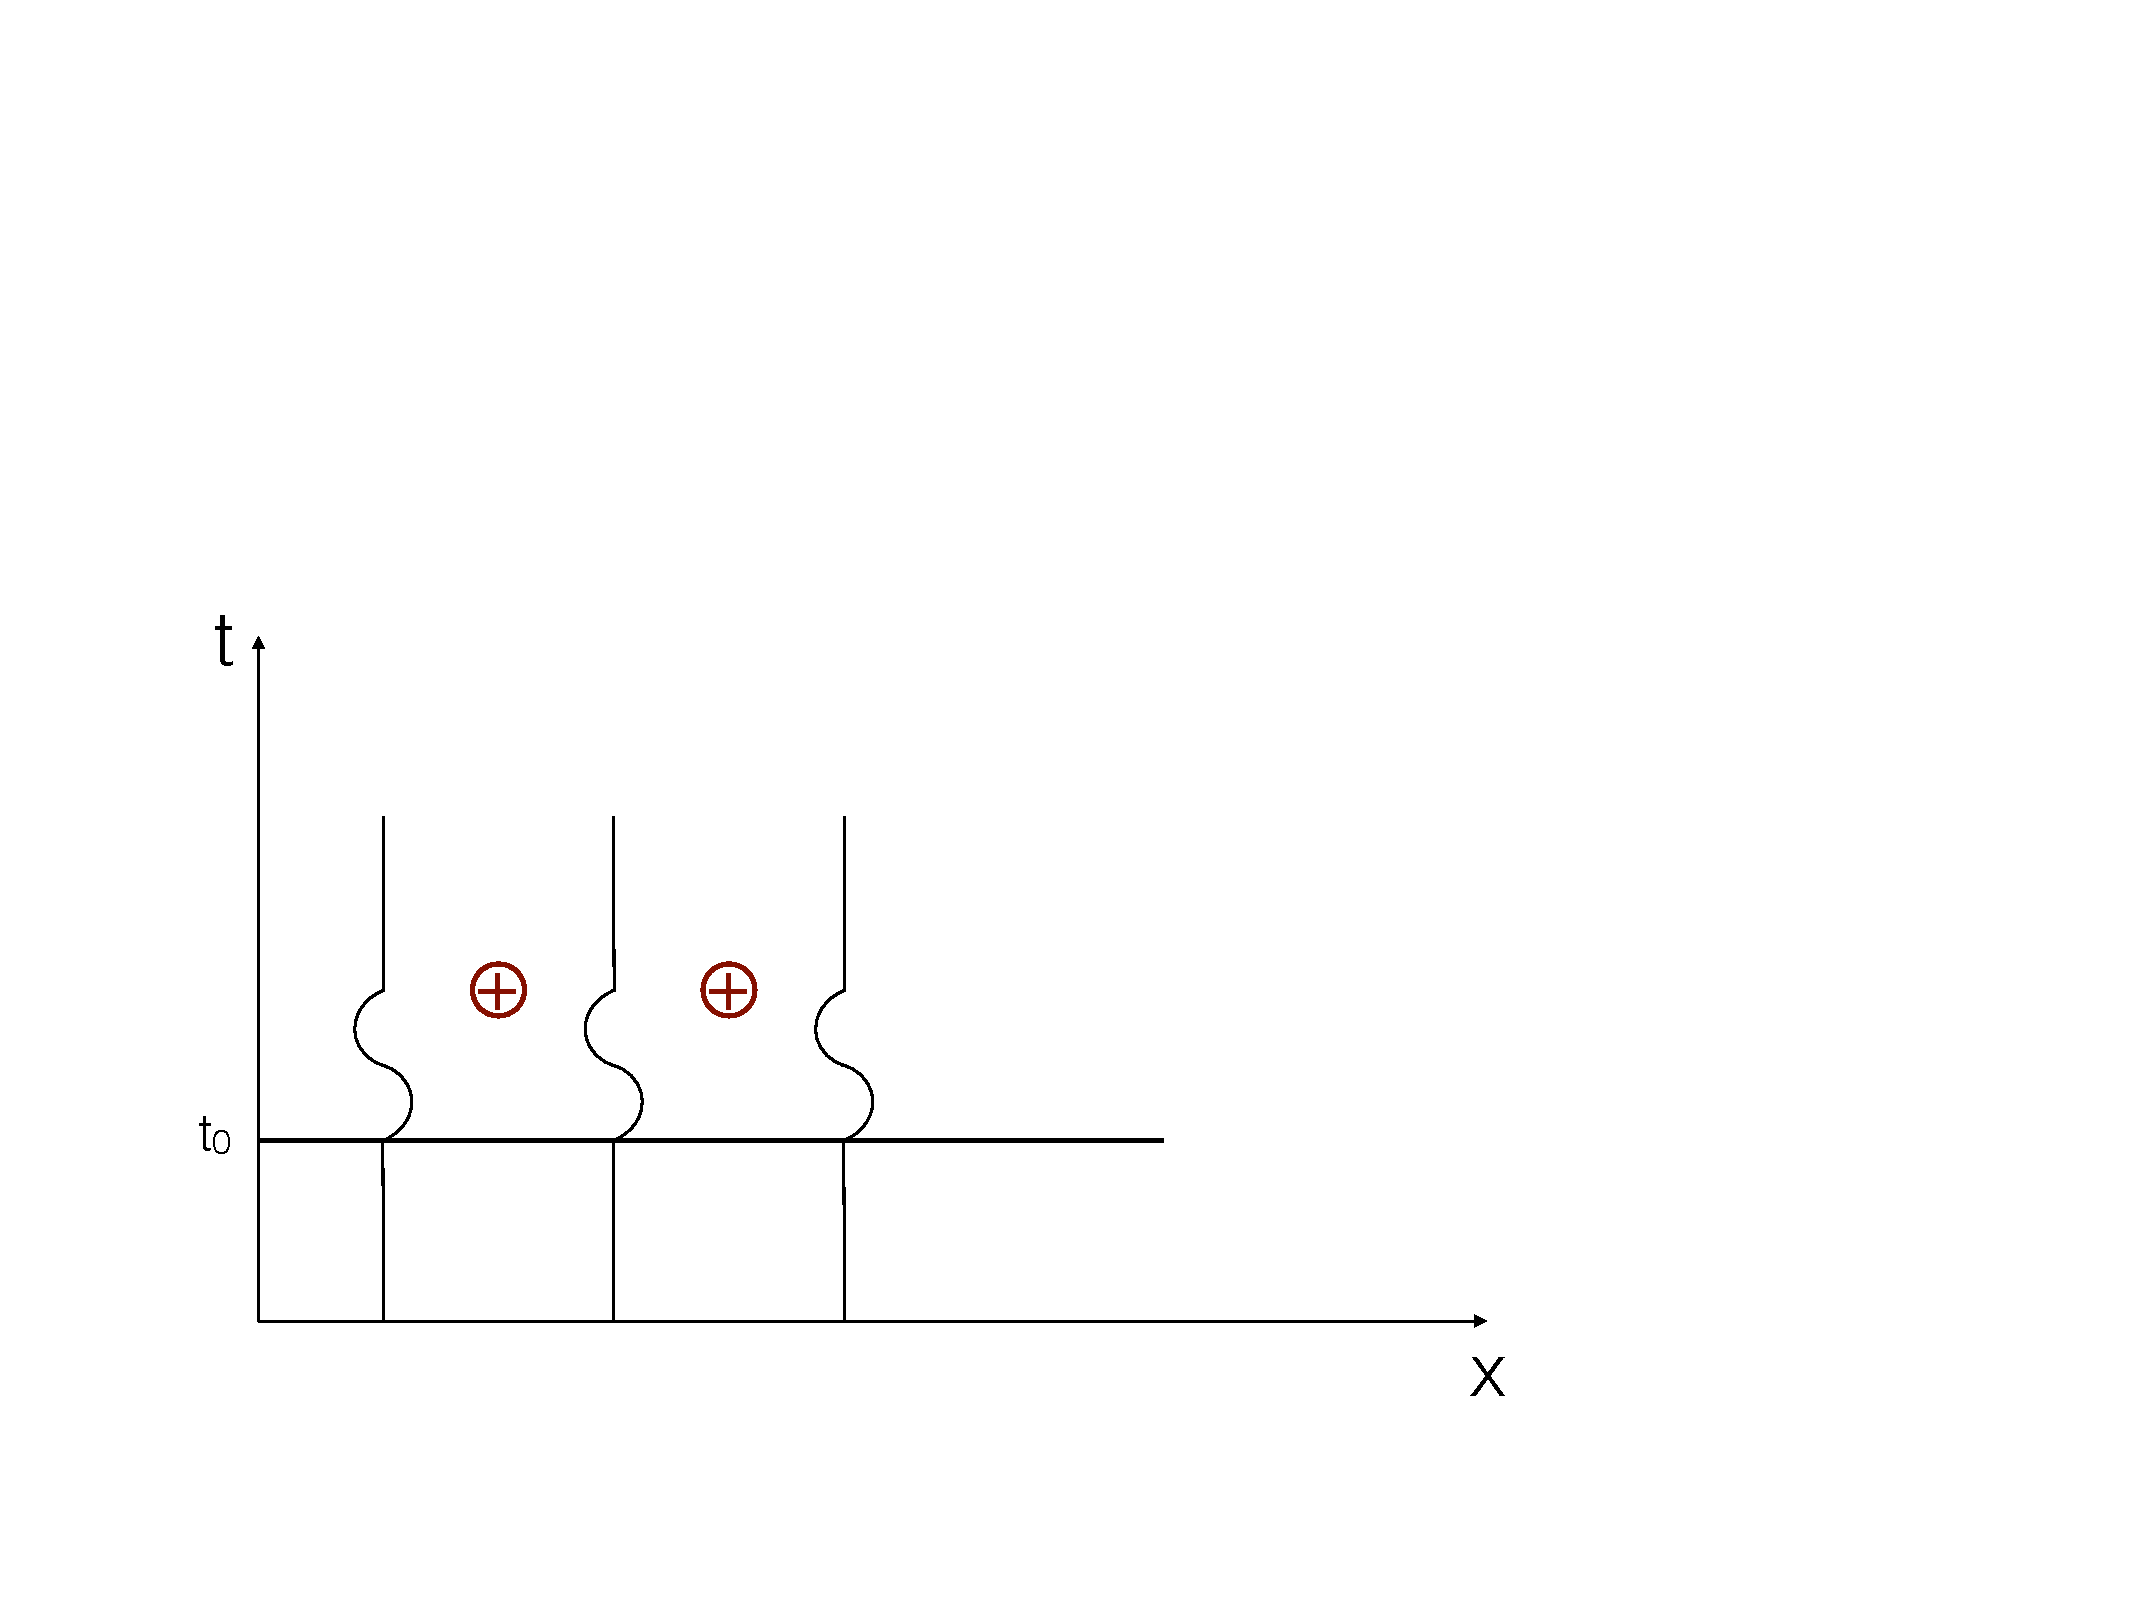
\includegraphics[width = \textwidth]{ReflexionsseismikBilder/Stapelung}
\end{figure}

\subsection{Berechnung der Schichtgeschwindigkeiten}

Trotz aller Maßnahmen zur Beseitigung der Mehrdeutigkeit ist unser Hauptziel noch nicht gelöst. Bisher haben wir nur die \textbf{Stapelgeschwindigkeiten} (Normal-Moveout-Geschwindigkeit) $v_{\text{nmo}}$, aber nicht die einzelnen \textbf{Intervallgeschwindigkeiten} $v_n$. Diese lassen sich jedoch einfach aus den Stapelgeschwindigkeiten berechnen. Der Zusammenhang wird durch die \textbf{Dix'sche Formel} beschrieben: \begin{equation*}
	v_n = \sqrt{\frac{v_{\text{nmo},n}^2 \cdot t_{0,n} - v_{\text{nmo},n-1}^2 \cdot t_{0,n-1}}{t_n - t_{n-1}}}
\end{equation*} 

 








	\chapter{Georadar}

Das Prinzip einer Messung mit Georadar ist ähnlich dem einer reflexionsseismischen Messung. 

Eine Georadar-Antenne sendet gepulste elektromagnetische Wellen aus, die an Grenzflächen reflektiert werden. Die reflektierten Wellen werden an der Oberfläche von einer zweiten Antenne empfangen.\\ 
Aus der Zeit zwischen Senden und Empfangen der Wellen, lässt sich die Geschwindigkeit der Wellen berechnen, sofern die Entfernung zum Reflektor (z.B. eine Gesteinsgrenze) bekannt ist. Aus dieser Geschwindigkeit lässt sich dann auf die elektromagnetischen Eigenschaften der Gesteine im Untergrund rückschließen.\\ 
In der Praxis ist es meist jedoch genau umgekehrt: die elektromagnetischen Eigenschaften des Untergrunds sind bekannt, daraus lassen sich dann wiederum die Geschwindigkeiten berechnen und daraus kann man die Entfernung des Reflektors ermitteln. 

Das Auflösungsvermögen sowie die Eindringtiefe der elektromagnetischen Wellen ist abhängig vom Frequenzbereich. Dieser liegt zwischen 10 und 100\,\si{MHz}. Grundsätzlich lässt sich sagen: je höher die Nominalfrequenz ist, desto feiner ist die Auflösung und desto geringer ist die Eindringtiefe. \\
Weiterhin ist die Eindringtiefe abhängig von der Leitfähigkeit der oberen Schichten. Liegt oben ein stark leitfähiges Material an, kann das Signal nicht in tiefere Schichten vordringen. 

Die Auswertung der gemessenen Daten erfolgt nach den Methoden der Reflexionsseismik.

Anwendung finden Georadarmessungen bei der Detektion von Höhlen und Spalten, bei der Ortung von Rohrleitungen, Kabeln, \dots und bei allgemeinen Untersuchungen zur Bodenstruktur.

\section{Messaufbau}
Der Messaufbau ist analog zum Messaufbau einer refraktionsseismischen Messung. Man unterscheidet auch hier wieder zwischen einer Messung mit Sender und Empfänger an einem Ort (\textbf{Monostatisch}) und einer Messung mit Distanz zwischen Sender und Empfänger (\textbf{Bistatisch}).


\begin{figure}[H]
	\begin{subfigure}[m]{0.5\textwidth}
	\centering
		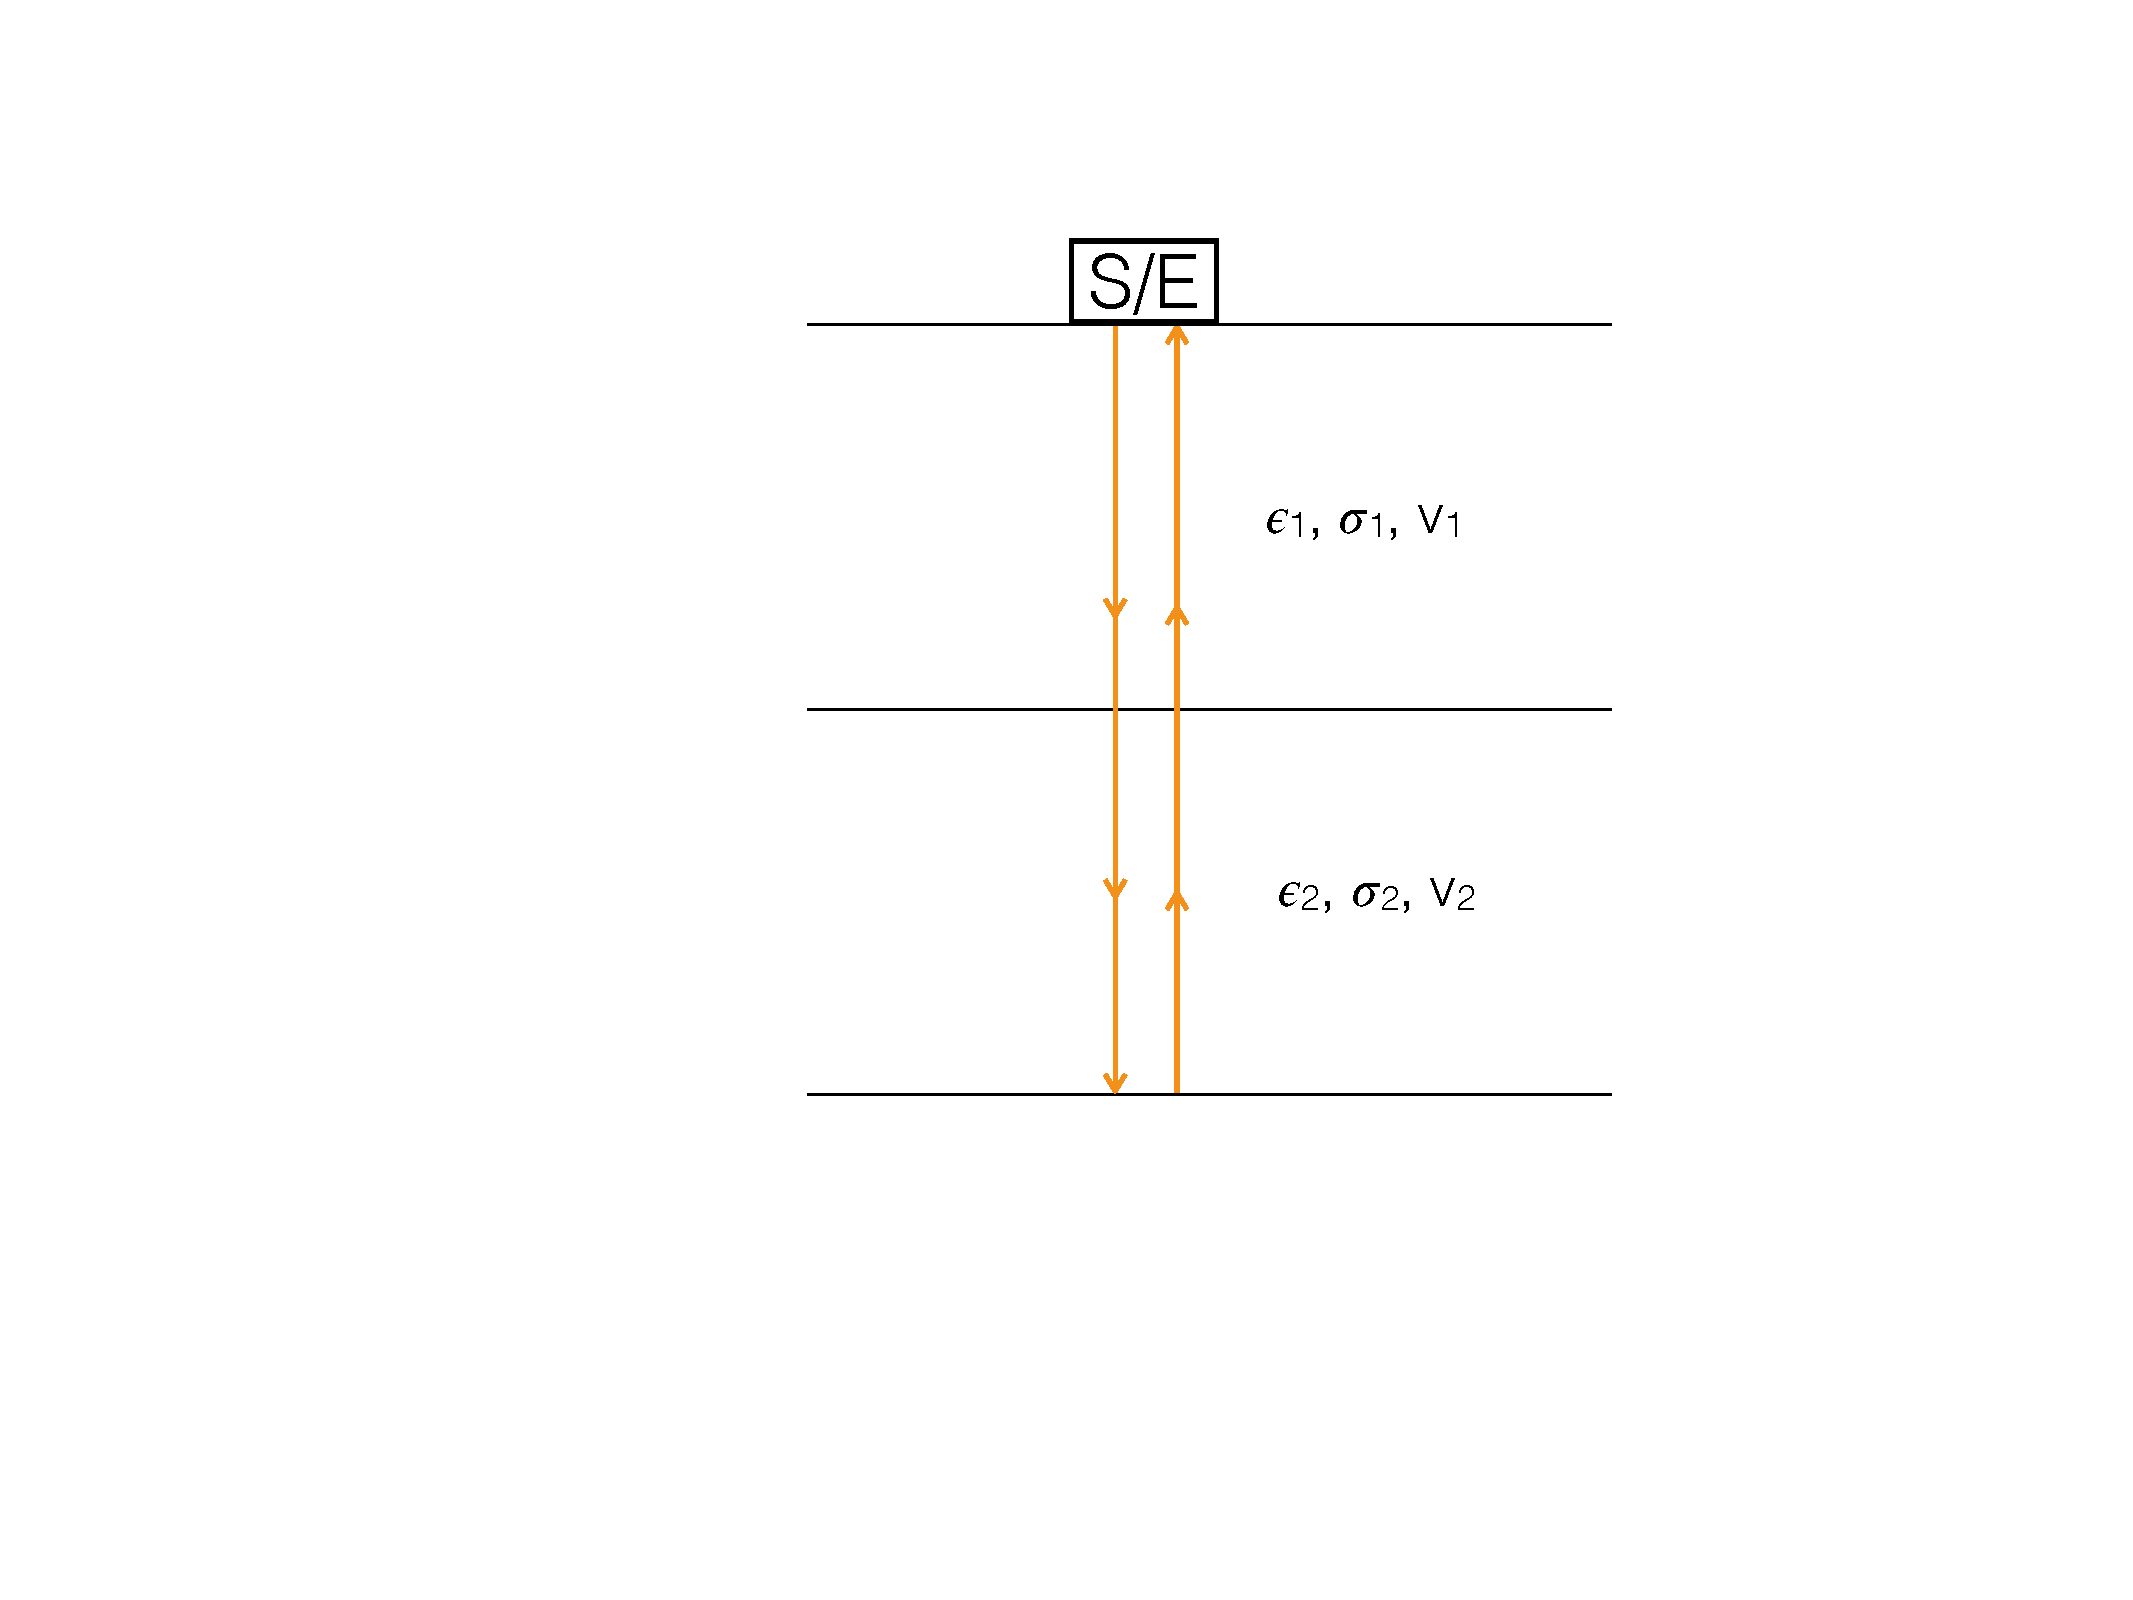
\includegraphics[scale = 0.3]{GeoradarBilder/Monostatisch}
	\caption*{monostatisch}	
	\end{subfigure}
	\begin{subfigure}[m]{0.5\textwidth}
	\centering
		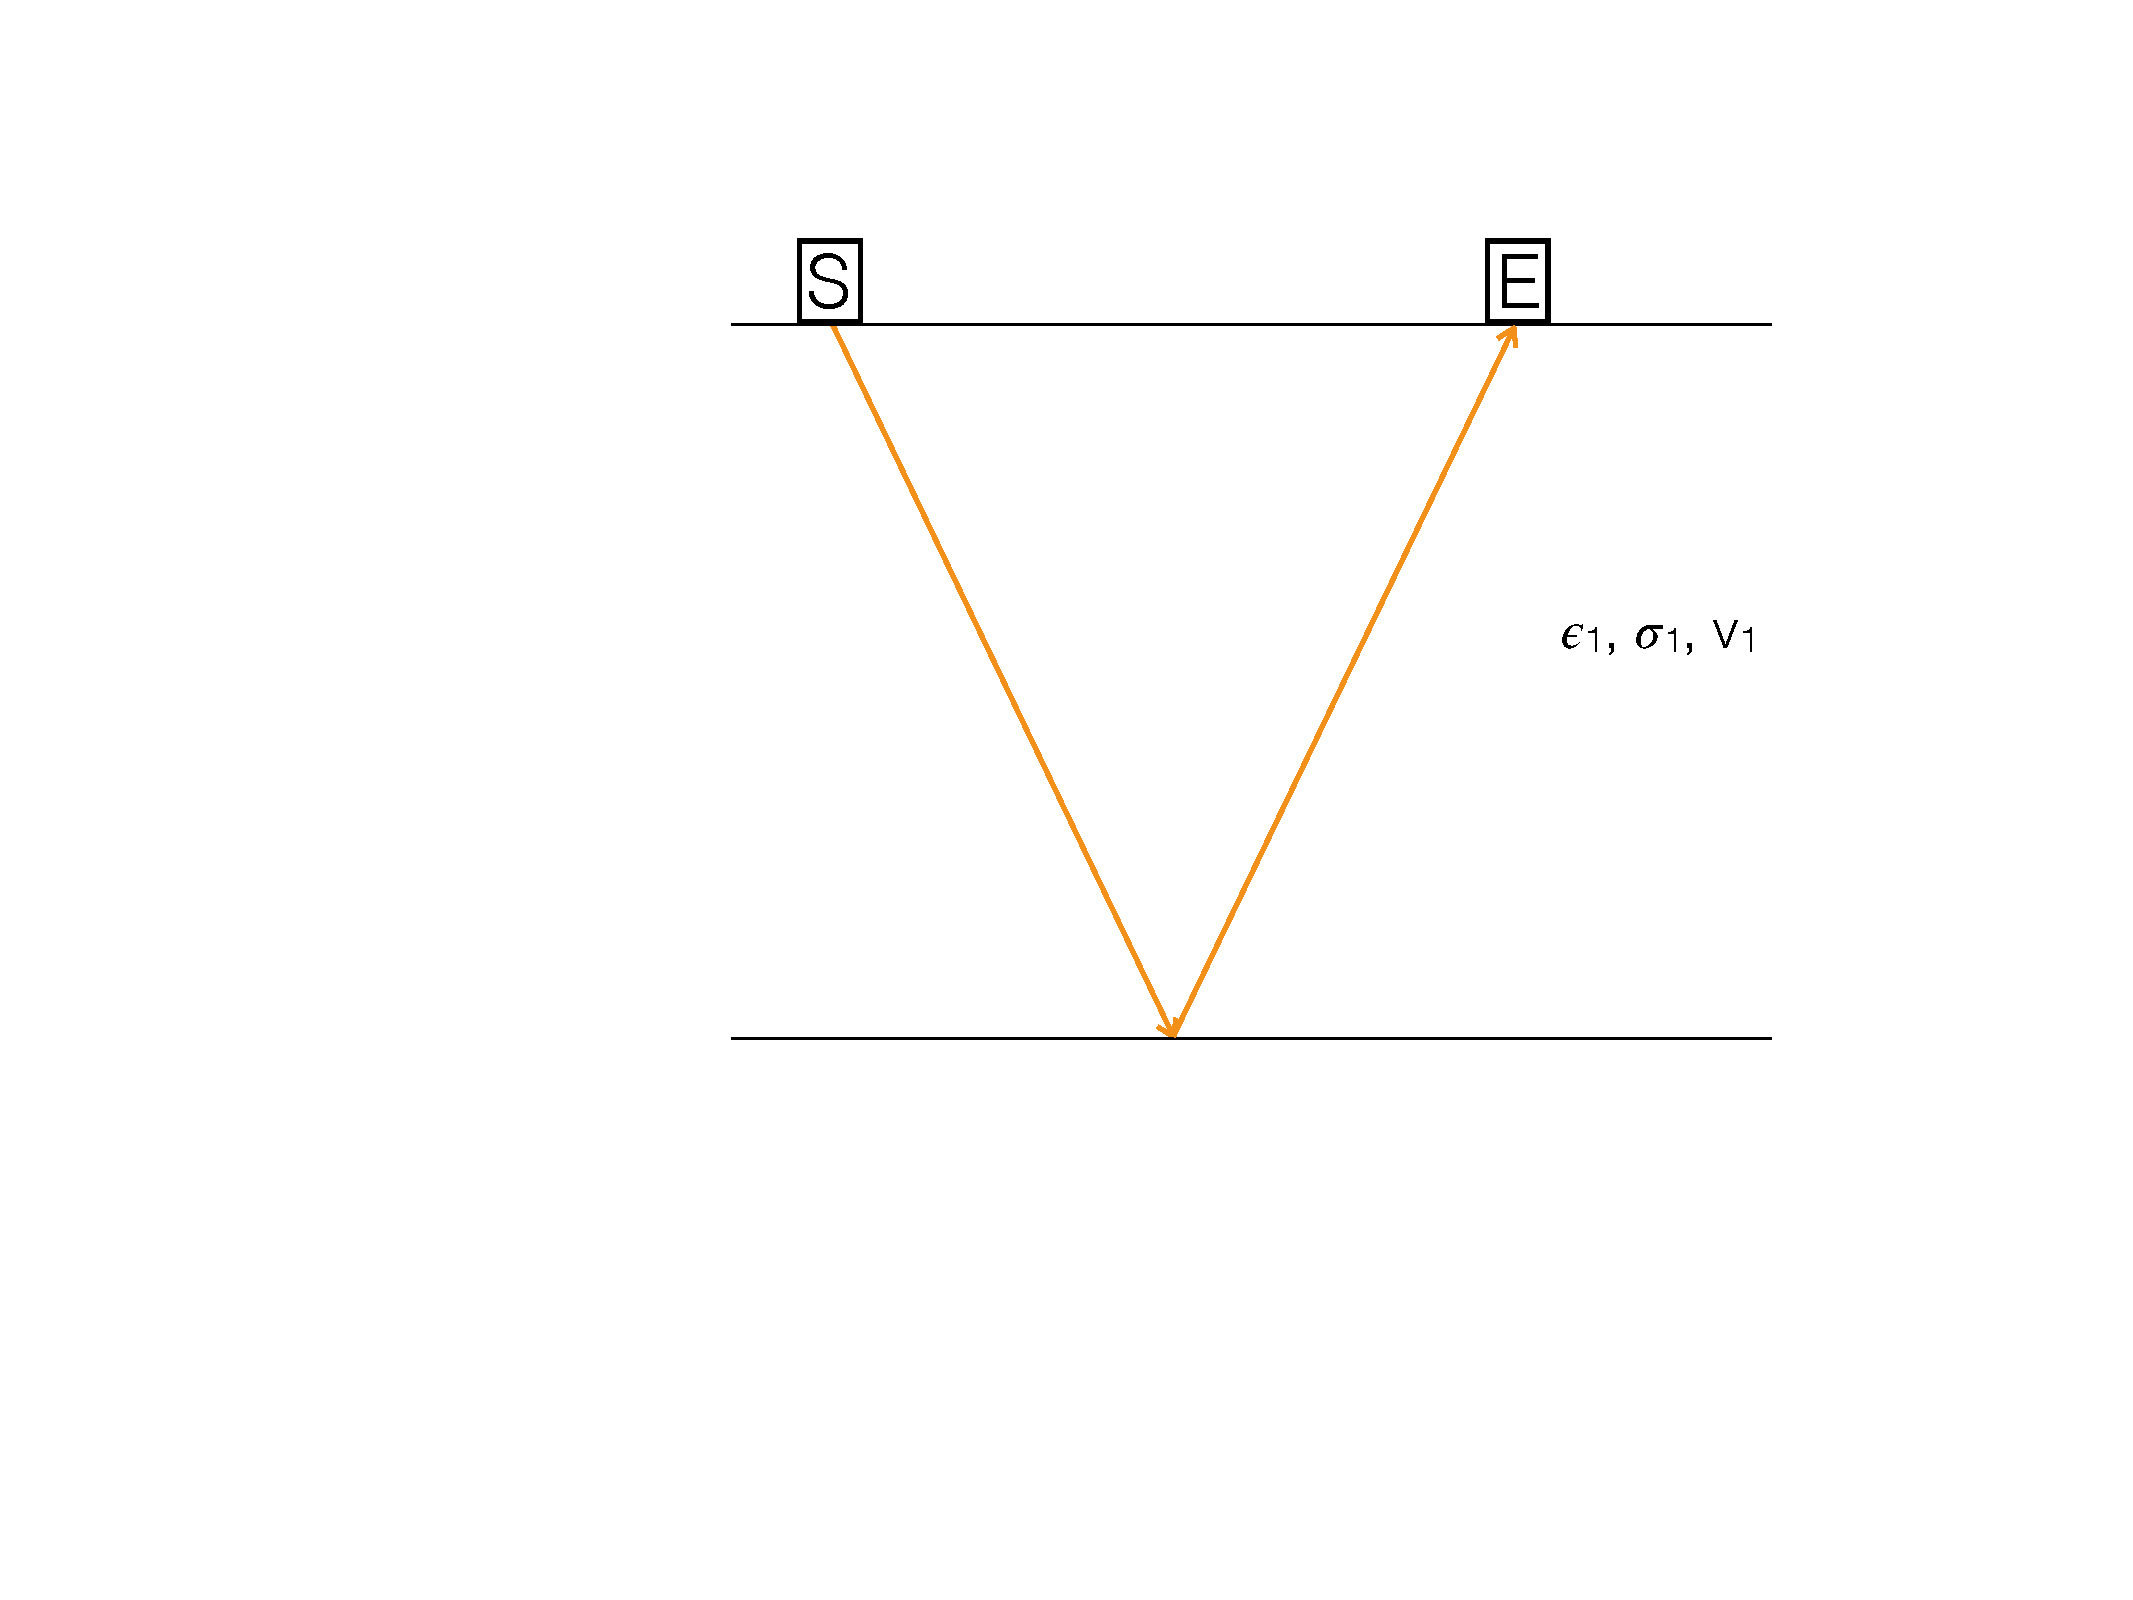
\includegraphics[scale = 0.3]{GeoradarBilder/Bistatisch}
	\caption*{bistatisch}
	\end{subfigure}
\end{figure}


Typisch für eine Messung ist ein bewegter monostatischer Messaufbau. Hierzu wird eine Sender-Empfänger-Kombination entlang einer Messlinie über die Messfläche gezogen. Durch die kontinuierliche Abstrahlung und Registrierung elektromagnetischer Wellen an Sender bzw. Empfänger kann man von einer steten Messung sprechen, d.h. das Messgebiet wird vollständig abgebildet. Die Messdaten werden in ein Radargramm übertragen.

\begin{figure}[H]
	\centering
	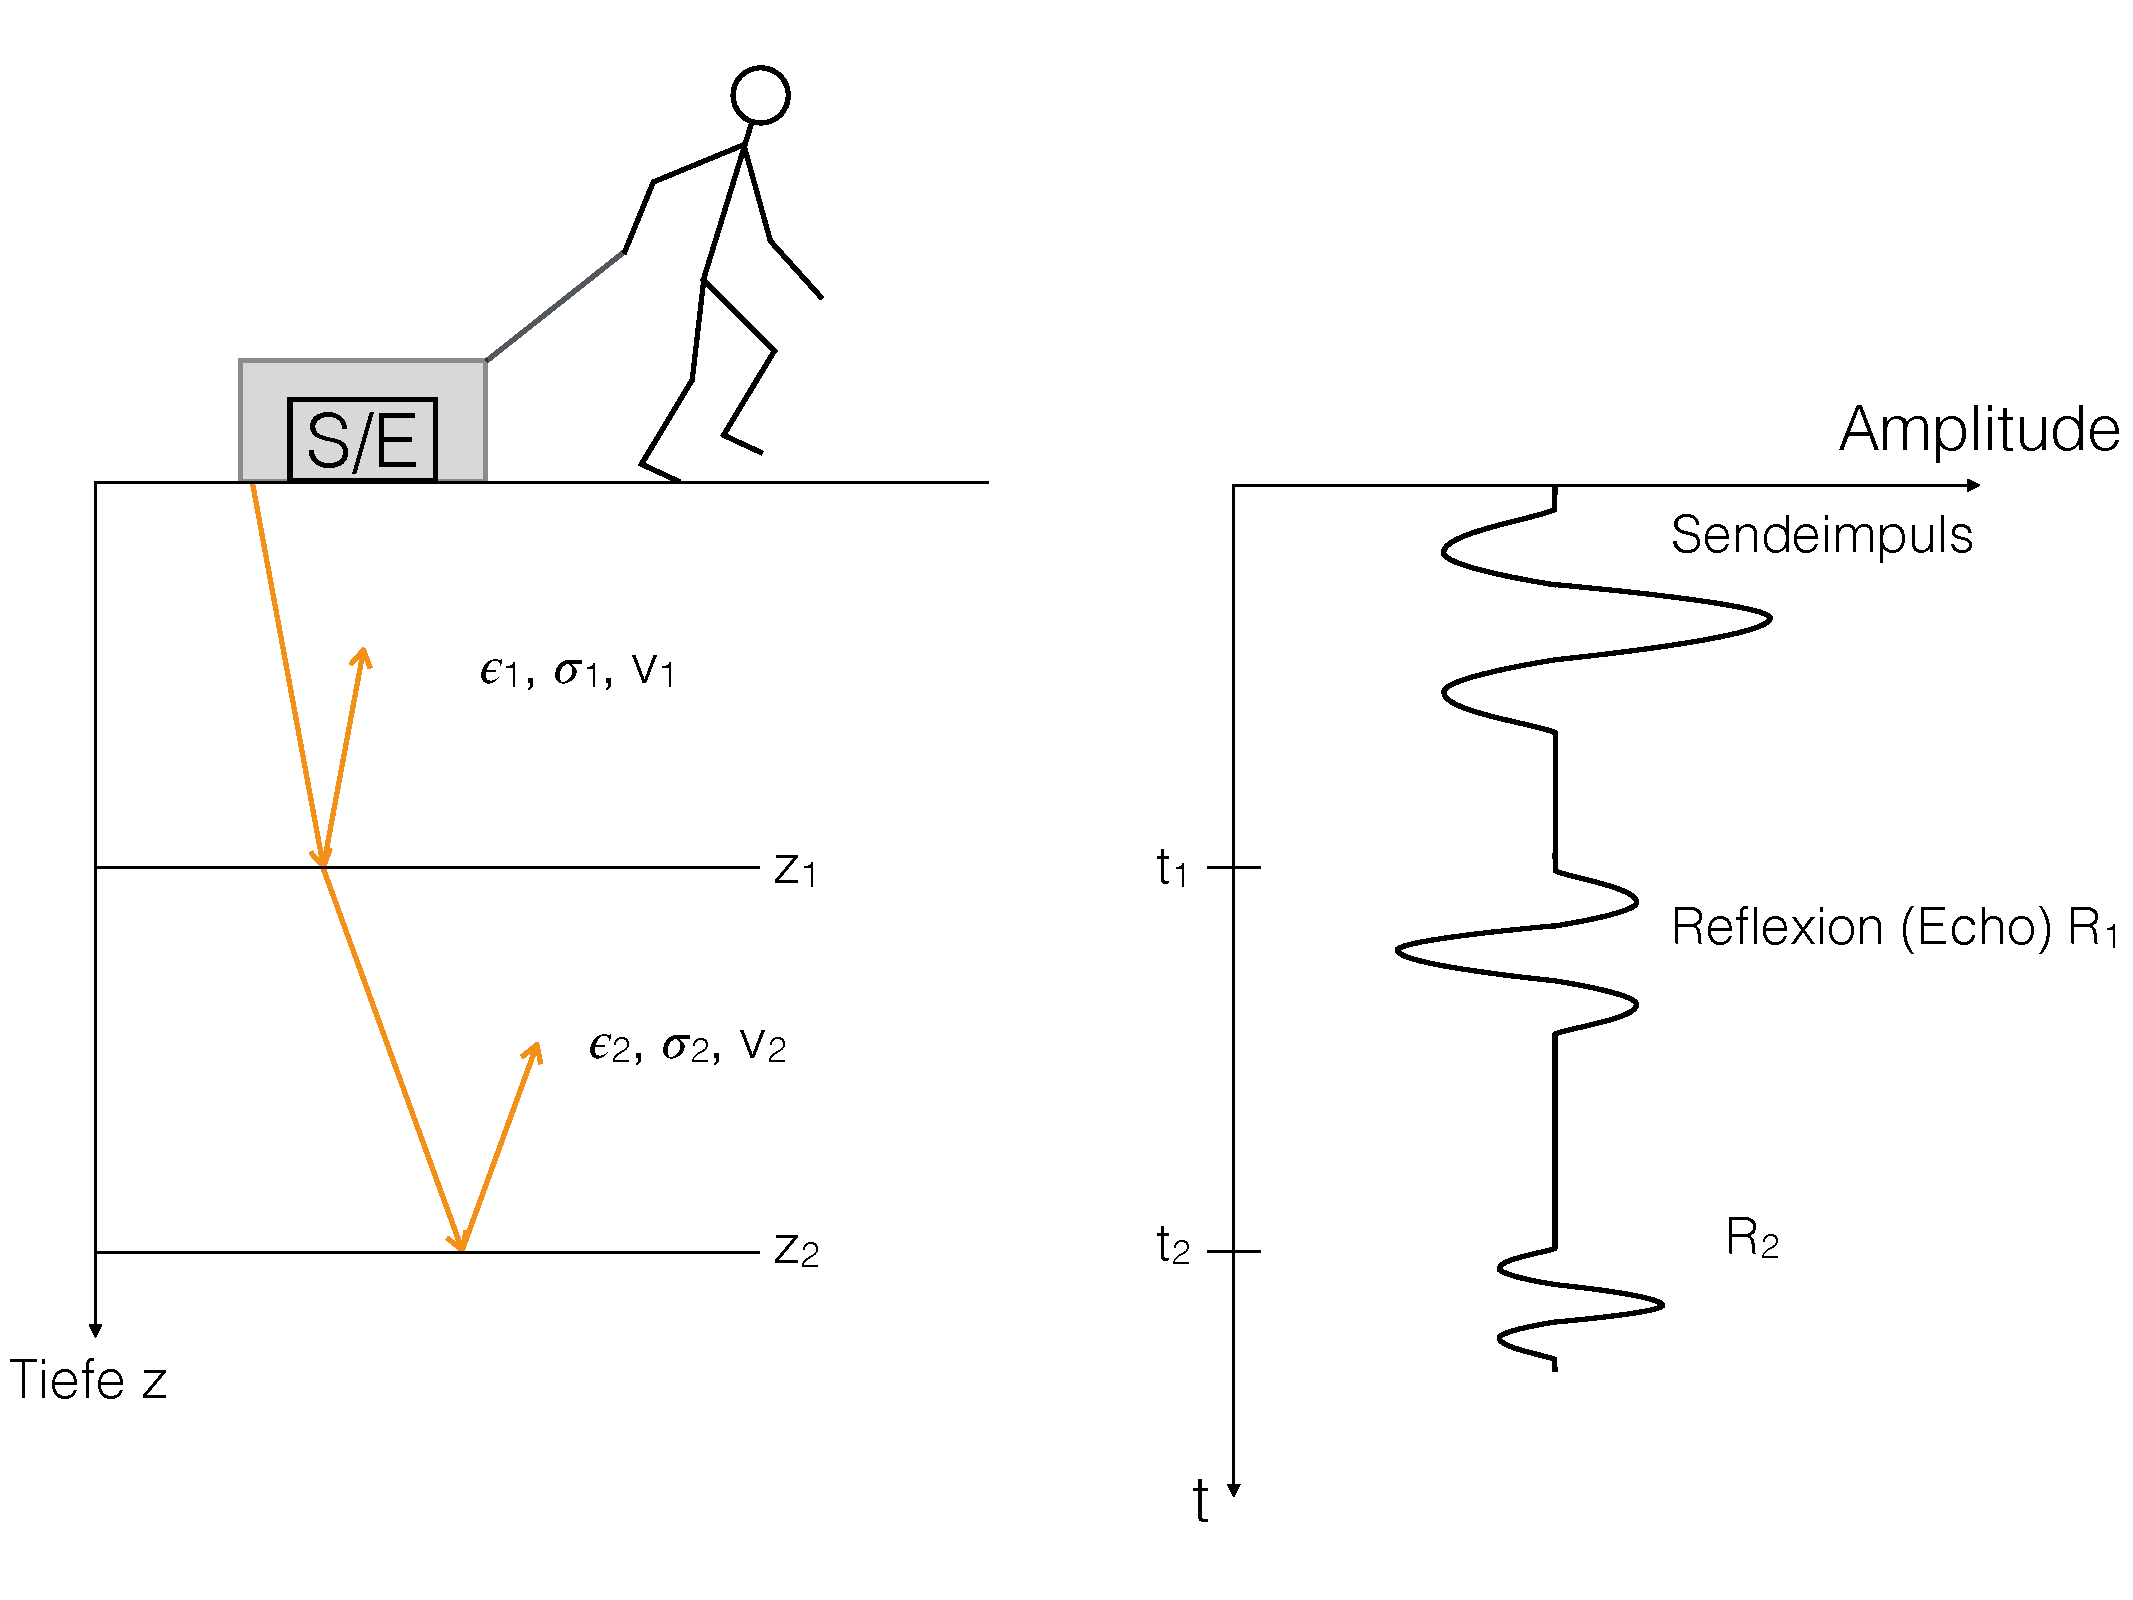
\includegraphics[width = \textwidth]{GeoradarBilder/bewegtMonostatisch}
\end{figure}


\section{Physikalische Parameter}
Die Leitfähigkeit eines Gesteins lässt sich durch zwei physikalische Konstanten beschreiben. Durch Kontrastunterschiede dieser beiden Materialeigenschaften $\epsilon$ und $\sigma$ im Untergrund entstehen Reflexionen und Diffraktionen (Beugungen) der elektromagnetischen Welle.

\subsubsection{Permittivität $\epsilon$} 
Legt man an ein Objekt ein elektrisches Feld an, beginnen sich die freien Ladungsträger des Objektes an diesem Feld auszurichten. Dabei erzeugen sie ein sogenanntes Polarisationsfeld, welches dem äußeren elektrischen Feld entgegenwirkt und dieses abschwächt. Wie stark das Polarisationsfeld wirkt wird mit Hilfe der Materialkonstante $\epsilon_r$ beschrieben. Die Permittivität berechnet sich dann so: \begin{equation*}
	\epsilon = \epsilon_r \cdot \epsilon_0
\end{equation*} Dabei ist $\epsilon_0$ die Permittivität des Vakuums.

\subsubsection*{Elektrische Leitfähigkeit $\sigma$}
Diese Materialgröße gibt an, wie fähig ein Stoff, ist Strom zu leiten.
Grundsätzlich gilt, dass stark wassergesättigte Gesteinsschichten oder tonhaltige Minerale stark leitfähig sind. Aus diesem Grund ist eine Georadarmessung bei solchen Gesteinsschichten nicht möglich.

\section{Auswertung}
Da die Auswertung der Daten aus einer Messung mit Georadar ähnlich der einer reflexionsseismischen Messung sind, möchten wir an dieser Stelle nur auf ein paar Besonderheiten eingehen. 

\subsection{Ausbreitungsgeschwindigkeit}
Wir betrachten zunächst den Normalfall: die Materialeigenschaften des Untergrundes sind bekannt und wir möchten die Geschwindigkeit der elektromagnetischen Wellen berechnen. Hierfür benutzen wir die folgende Formel: \begin{equation*}
	v = \frac{c}{\sqrt{\mu_r \cdot \epsilon_r}} \approx \frac{c}{\sqrt{\epsilon_r}}
\end{equation*}
Hierbei ist $\epsilon_r$ die relative Permittivität, die wir bereits kennengelernt haben. $c$ bezeichnet die Vakuumlichtgeschwindigkeit mit einem Wert von gerundet $3 \cdot 10^{8}\,\si{m/s}$. Die relative Permeabilität wird mit $\mu_r$ angegeben. Dieser Wert ist nur gering variabel und bewegt sich um den Wert 1. Der beeinflussende Faktor für die Wellengeschwindigkeit ist also relative Permittivität. $\epsilon_r$ variiert zwischen Werten von 1 bis 81.

\subsection{Auflösungsvermögen}
Interessant bei einer Messung mit Georadar ist das Auflösungsvermögen der verwendeten Antenne. Dazu muss zunächst der Begriff der \textbf{Nominalfrequenz} geklärt werden. Georadar-Antennen strahlen ihre Energie über eine Bandbreite ab und nicht nur über exakt eine Frequenz. Der Mittelwert dieser Bandbreite ist Nominalfrequenz $f_{\text{N}}$, bei welcher die Antenne also maximal viel Energie abgibt.

Maßgebend für das Auflösungsvermögen ist die räumliche Ausdehnung des elektromagnetischen Pulses (\textbf{Wellenlänge}): \begin{equation*}
	\lambda = \frac{1}{f_{\text{N}}} \cdot v = T \cdot v
\end{equation*} Hierbei ist $v$ die Geschwindigkeit der Radarwelle und T die Pulslänge.

Die theoretische vertikale Auflösung $r$ berechnet sich nun als ein Viertel der Wellenlänge: \begin{equation*}
	r = \frac{1}{4} \lambda
\end{equation*}

\subsection{Auswertung von Diffraktionen}
Trifft die elektromagnetische Welle auf eine kleinräumige Diskontinuität im Untergrund (zum Beispiel eine Rohrleitung, keine Grenzschicht) wird sie wie eine seismische Welle gebrochen und ein Teil wird reflektiert. Diese rückläufige Welle wird an der Oberfläche registriert. Unter der Annahme, dass die Geschwindigkeit $c$ im Medium konstant ist, lässt sich die Tiefe der Diffraktion bestimmen, bzw. umgekehrt die Geschwindigkeit der Welle. Die Formel zur Berechnung wollen wir nun mit Hilfe einer Veranschaulichung des Messaufbaus herleiten.


\begin{figure}[H]
	\centering
	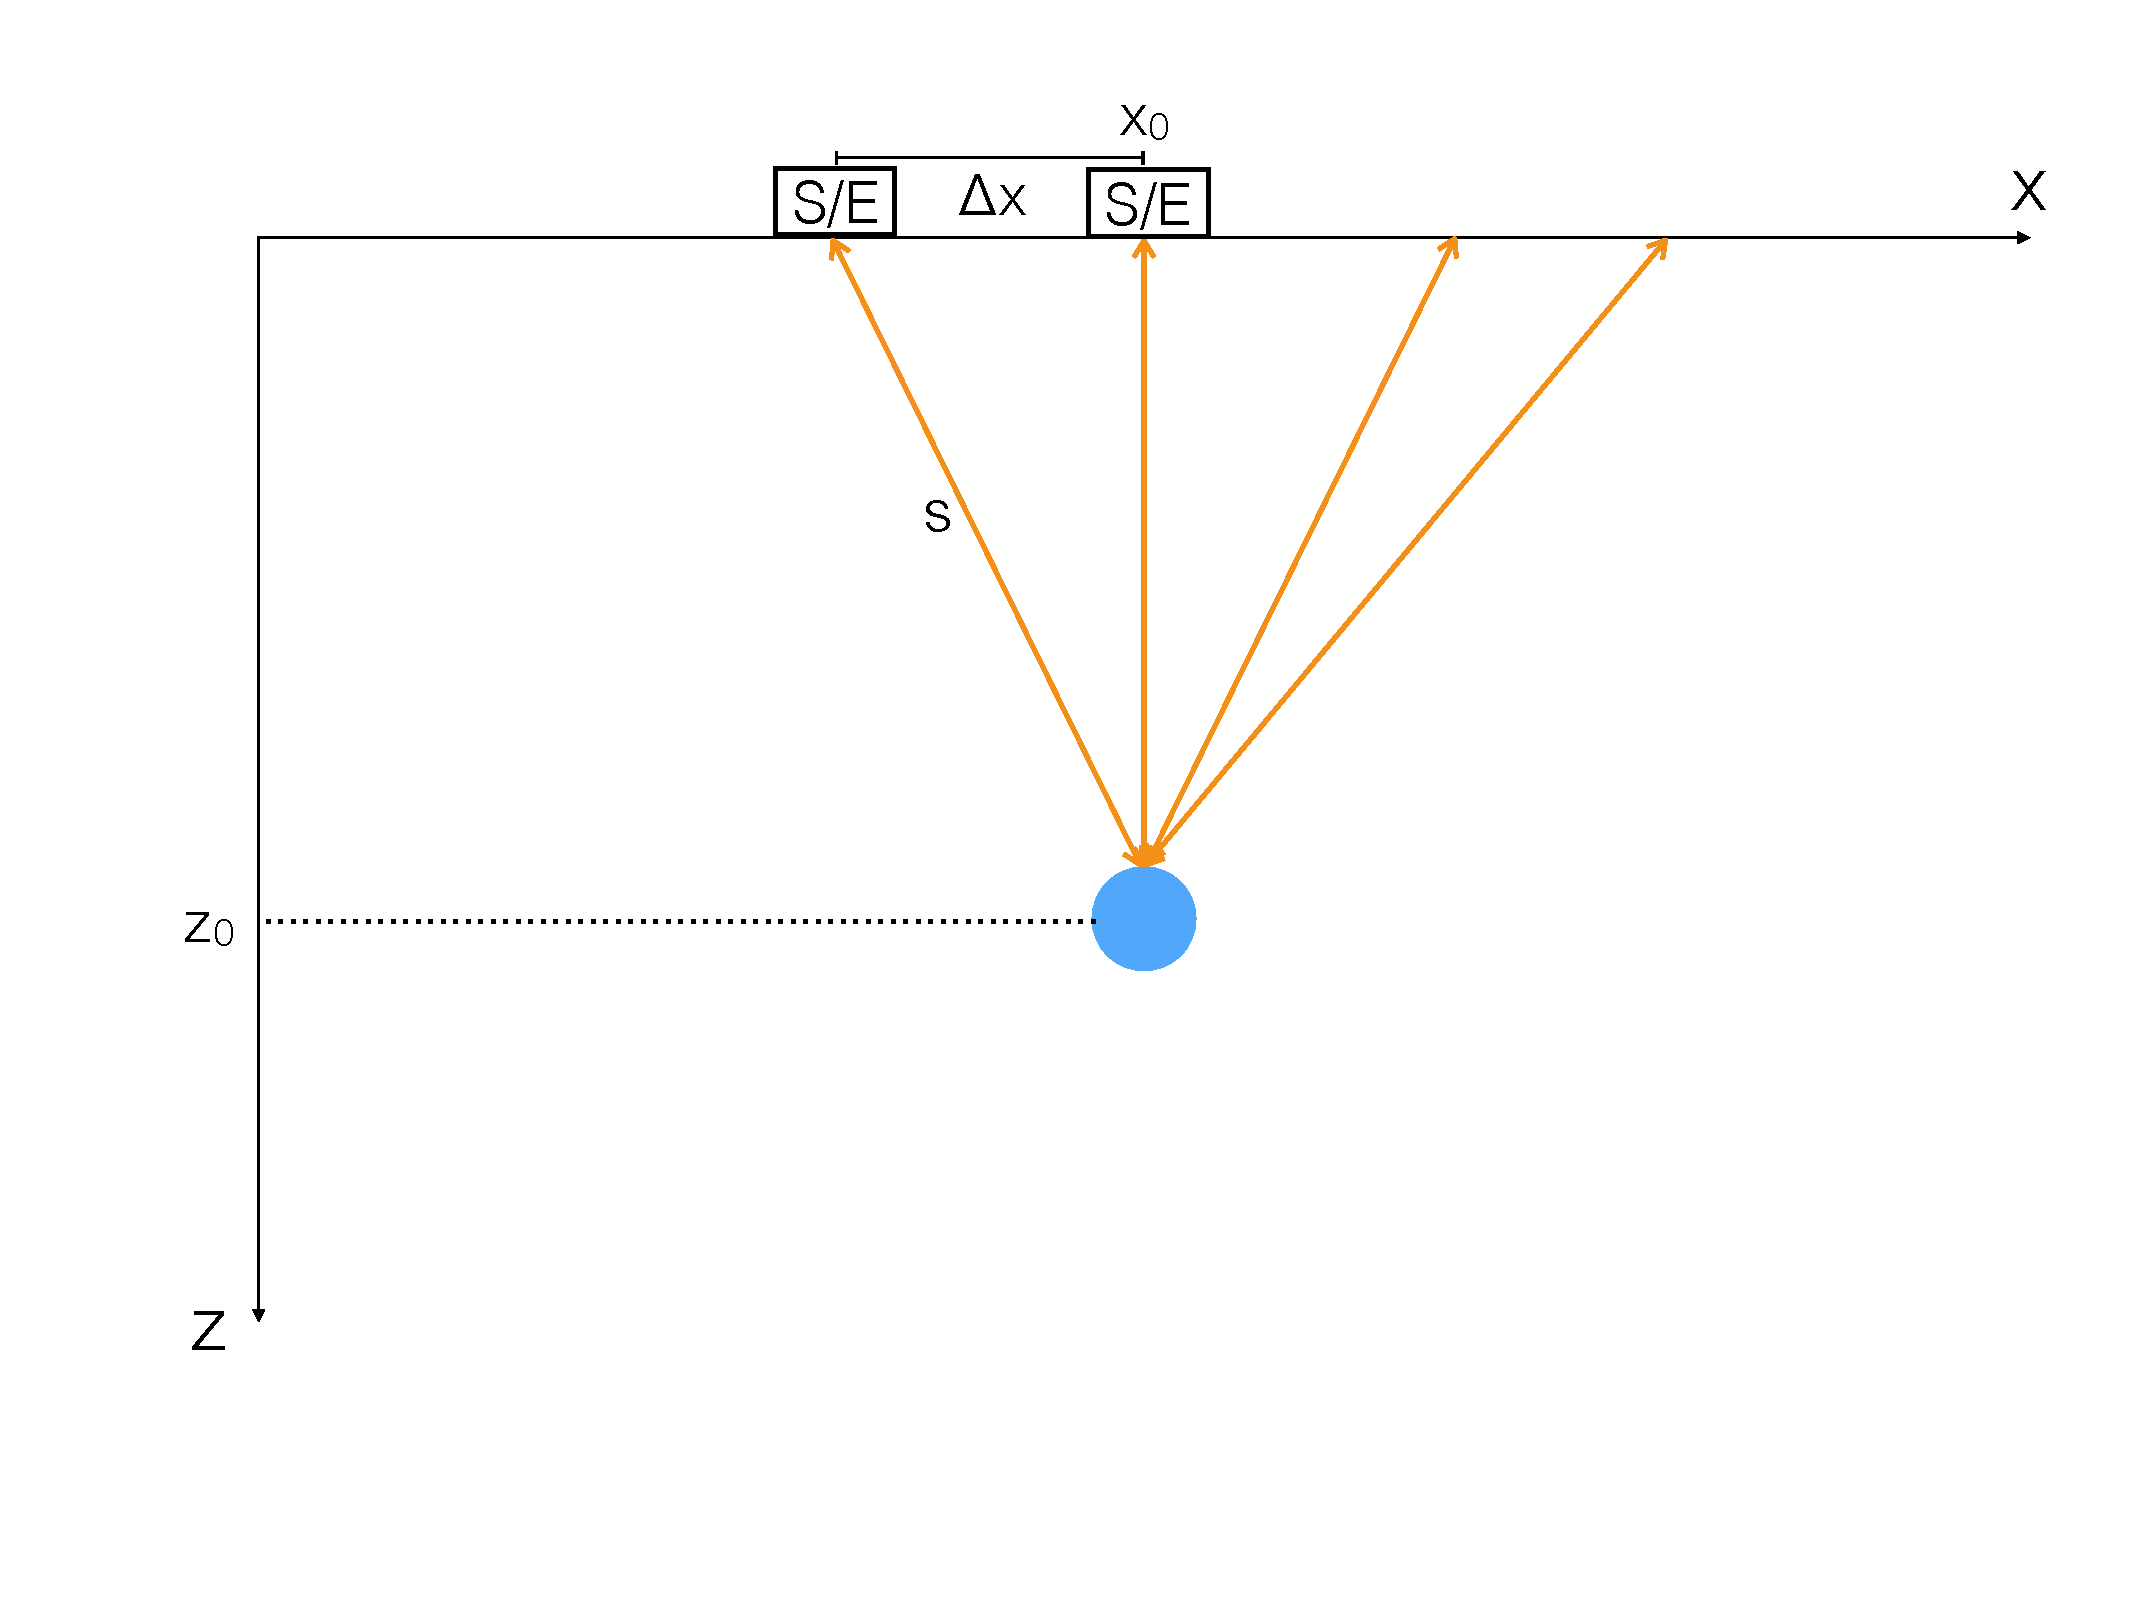
\includegraphics[width = \textwidth]{GeoradarBilder/DiffraktionAufbau}
\end{figure}


Die Laufzeit $t$ berechnet sich so: \begin{equation*}
	t = \frac{2 \cdot s}{v}
\end{equation*}

Diese Gleichung lässt sich unter Kenntnis der Standorte von Sender und Empfänger umformulieren: \begin{equation*}
	t = \frac{2}{v} \cdot \sqrt{\Delta x^2 + z_0^2} = \frac{2}{v} \cdot \sqrt{(x-x_0)^2 + z_0^2}
\end{equation*}

Misst man nun auch noch die Laufzeit $t_0$ der Welle, die im 90$^\circ$-Winkel zur Oberfläche vom Empfänger abstrahlt, lässt sich $z_0$ berechnen: \begin{equation*}
	t_0 = \frac{2 \cdot z_0}{v} \quad \Rightarrow \quad z_0 = \frac{t_0 \cdot v}{2}
\end{equation*}

Daraus ergibt sich nun die Laufzeitgleichung: \begin{equation*}
	t^2 = \frac{4}{v^2} \cdot (\Delta x^2 + z_0^2) = \frac{4}{v^2} \cdot \Delta x^2 + t_0^2
\end{equation*}

Die Gleichung für $t$ ergibt beim Auftragen eine Hyperbel, welche Diffraktionshyperbel genannt wird. 


\begin{figure}[H]
	\centering
	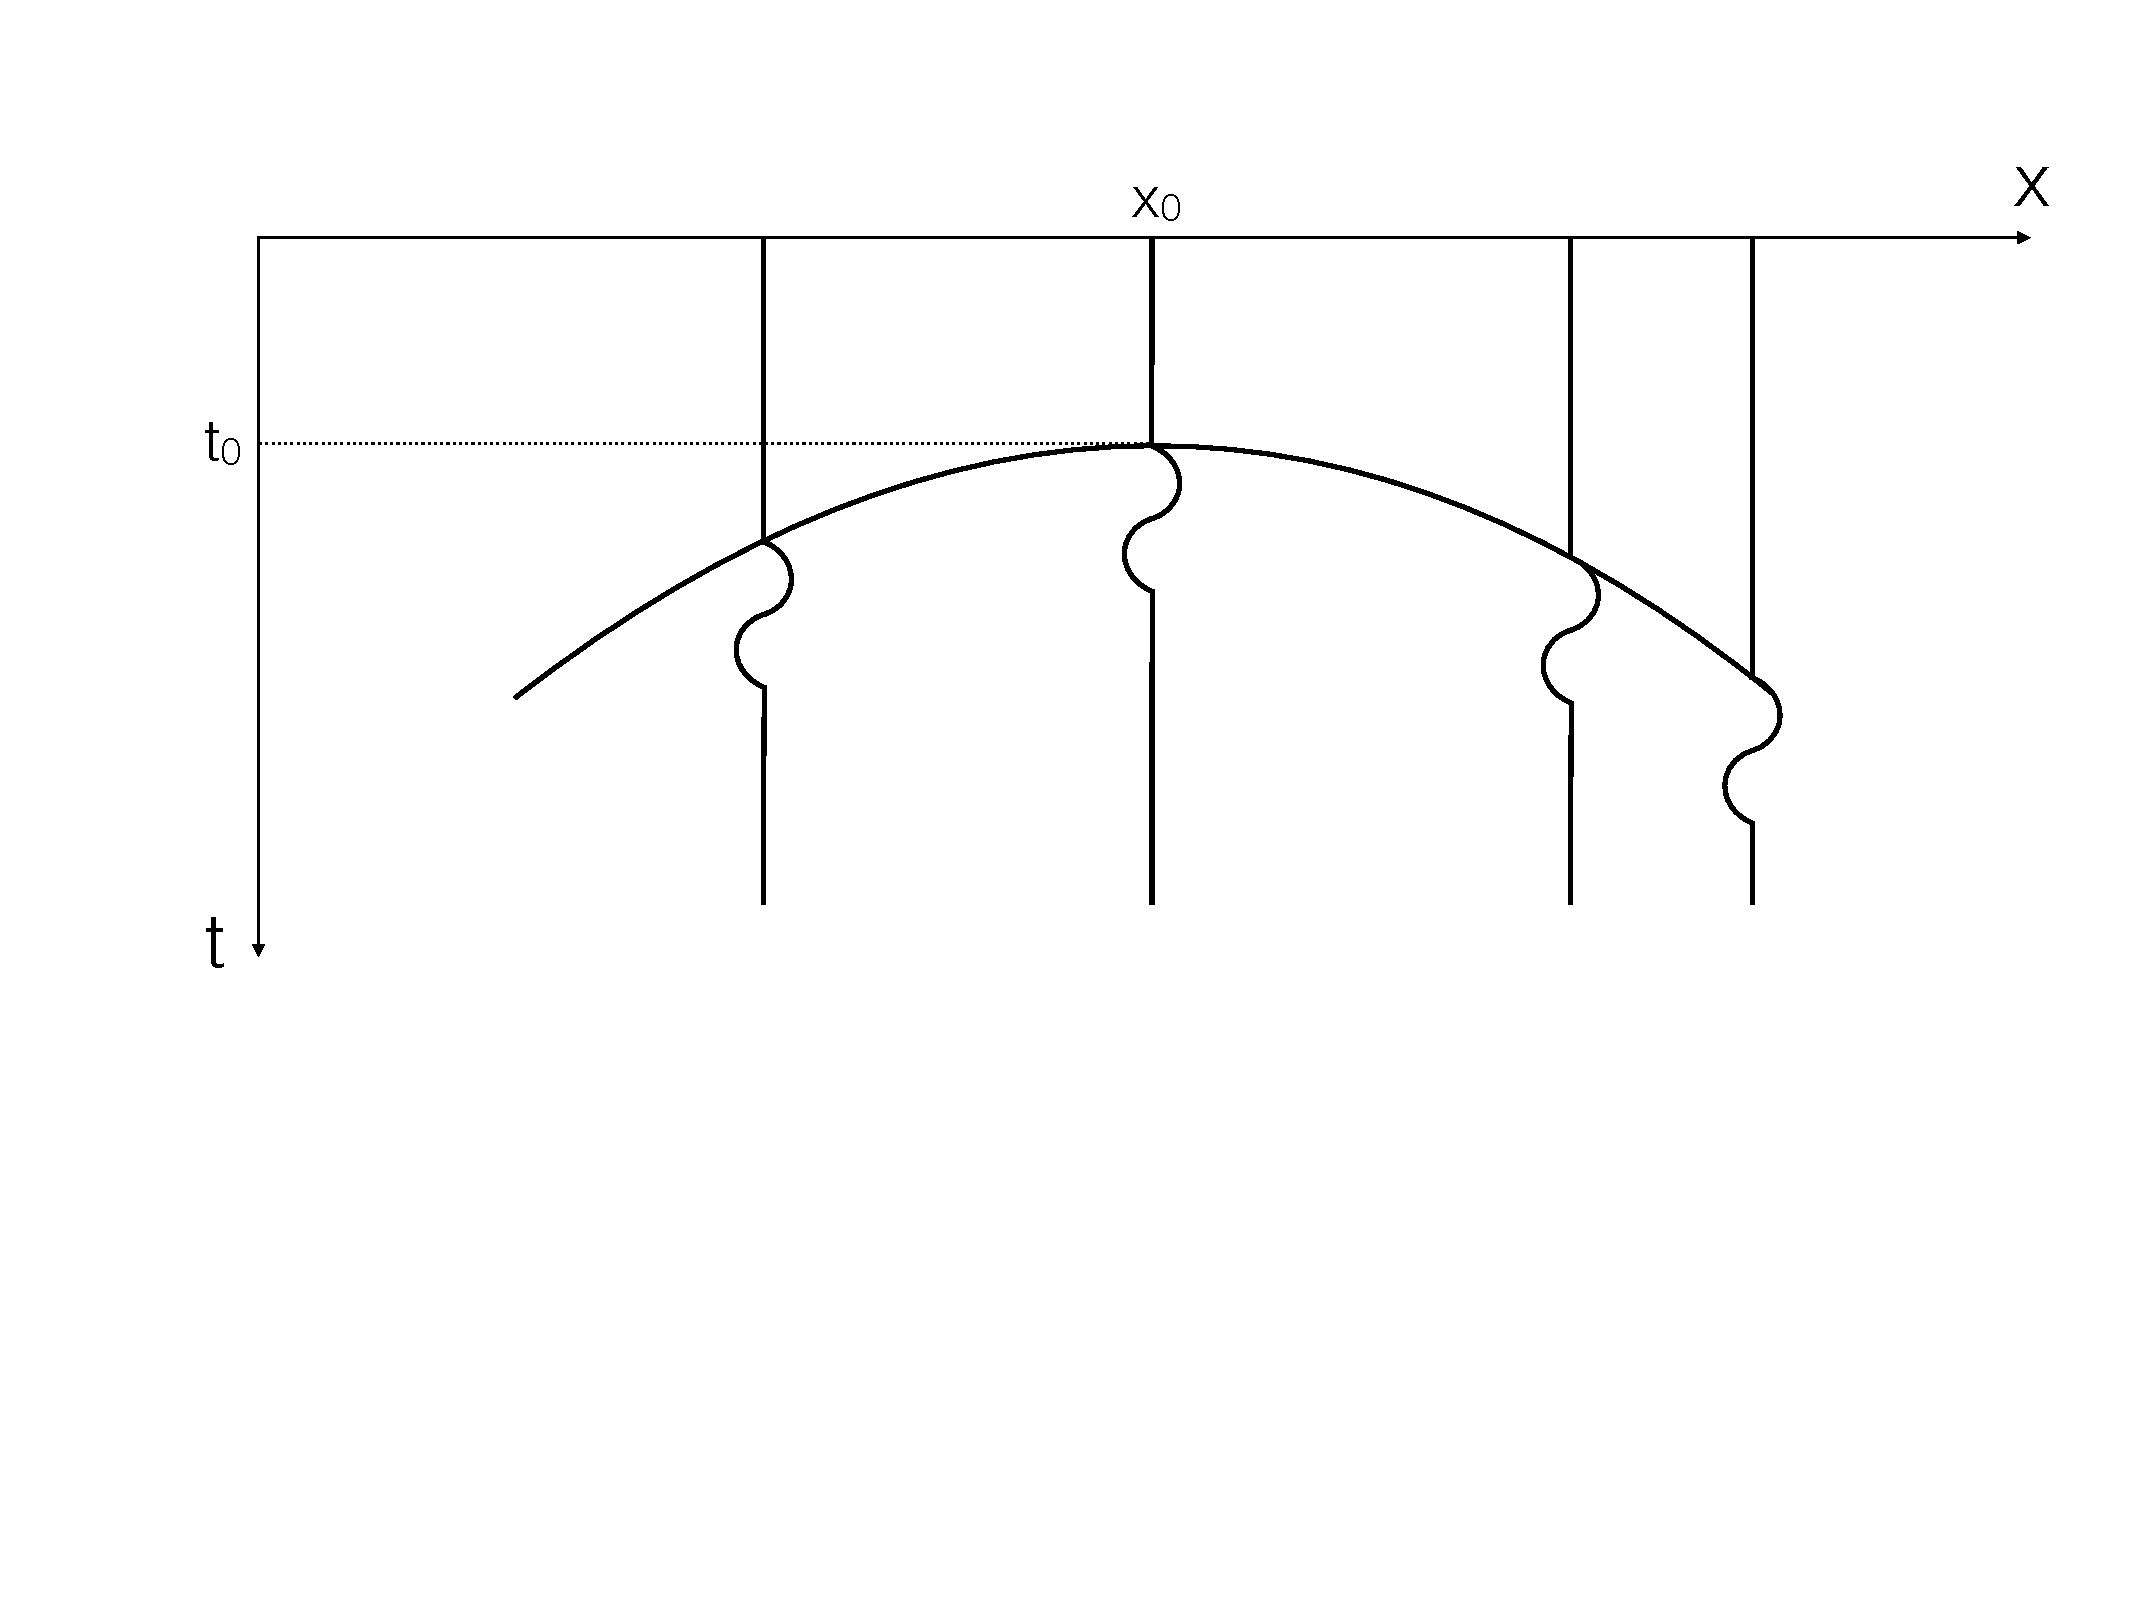
\includegraphics[width = \textwidth]{GeoradarBilder/Radargramm}
\end{figure}

Aus Kenntnis der Geschwindigkeit lassen sich Rückschlüsse über die Materie des Untergrunds ziehen.


\subsection{Reflexionskoeffizient}
Eine weitere Möglichkeit zur Analyse bietet die Reflexionsstärke. Hierbei legt man zu Grunde, dass sich die Permittivität $\epsilon$ an der Grenzschicht signifikant ändert. Der Reflexionskoeffizient lässt sich annähern durch: \begin{equation*}
	R = \frac{\sqrt{\epsilon_2 - \epsilon_1}}{\sqrt{\epsilon_2 + \epsilon_1}}
\end{equation*}

Dies ist die gängige Methode bei Messungen im Feld.















	\chapter{Geoelektrik}
Geoelektrische Verfahren dienen zur Erforschung der Erdkruste durch Messung elektrischer Spannung und Stromstärke an der Erdoberfläche. Hierbei wird zwischen künstlichen und natürlichen Messmethoden unterschieden.

Anwendung findet die Geoelektrik hauptsächlich bei ingenieurgeophysikalischen Fragestellungen, wie beispielsweise die Erkundung möglicher Lecks in Rohrleitungen, Deponieuntersuchungen oder Untersuchungen des Grundwasservorkommens. Geoelektrische Messungen werden auch verwendet bei globalen Forschungsfragen wie die Untersuchung von Gletschern oder Permafrostböden.

\section{Messmethoden}
\subsection{Künstliche Quellen}
\subsubsection{Gleichstromverfahren}
Durch eine externe Spannungsquelle wird ein künstliches Gleichstromfeld an die Erde angelegt. Sind der Wert der Spannung $U$ und Stromstärke $I$ bekannt, kann der spezifische Widerstand gemessen werden. Dieser Widerstand ist eine Gesteinseigenschaft. Ist der Untergrund nicht homogen, wird der scheinbare spezifische Widerstand gemessen, welcher vom spezifischen Widerstand verschieden ist.

\subsubsection{Wechselstromverfahren}
Ein künstlich angelegtes elektromagnetisches Wechselfeld induziert Ströme in der Erde. Durch Messung des dadurch induzierten elektromagnetischen Feldes an der Erdoberfläche lassen sich Rückschlüsse auf die Gesteinseigenschaften des Untergrundes ziehen.

\subsection{Natürliche Quellen}
\subsubsection{Eigenpotentialverfahren}
Bei dieser Methode werden die oberflächennahen Gleichstromfelder gemessen. Solche Felder entstehen beispielsweise durch Kontaktspannungen im Bereich von Erzlagerstätten.

\subsubsection{Magnetotellurik}
Durch Sonnenaktivität, Blitze oder Ähnliches schwankt das elektromagnetische Feld der Erde. Dadurch wird auch das lokale elektromagnetische Feld verändert. Diese Veränderung wird bei der Magnetotellurik vermessen.

\section{Messkonfigurationen}
Die am häufigsten verwendete Messmethode ist das künstliche Gleichstromverfahren, weshalb wir im Folgenden auf diese näher eingehen.

Messungen mit künstlicher Stromzufuhr verwenden eine Vierpunktanordnungen. Diese umfasst zwei Elektroden A und B, über welche der Strom zugeführt wird, und zwei Messsonden M und N zur Potentialmessung. Diese Elektroden und Sonden werden meist in einer Linie angeordnet. Der Abstand zueinander ist hierbei vom gewünschten Untersuchungsergebnis abhängig.

\subsection{beliebige Vierpunktanordnung}
Diese Anordnung unterliegt keiner Regel. Auch sind die Elektroden nicht zwingend in Linie angeordnet. 

\begin{figure}[H]
	\centering
	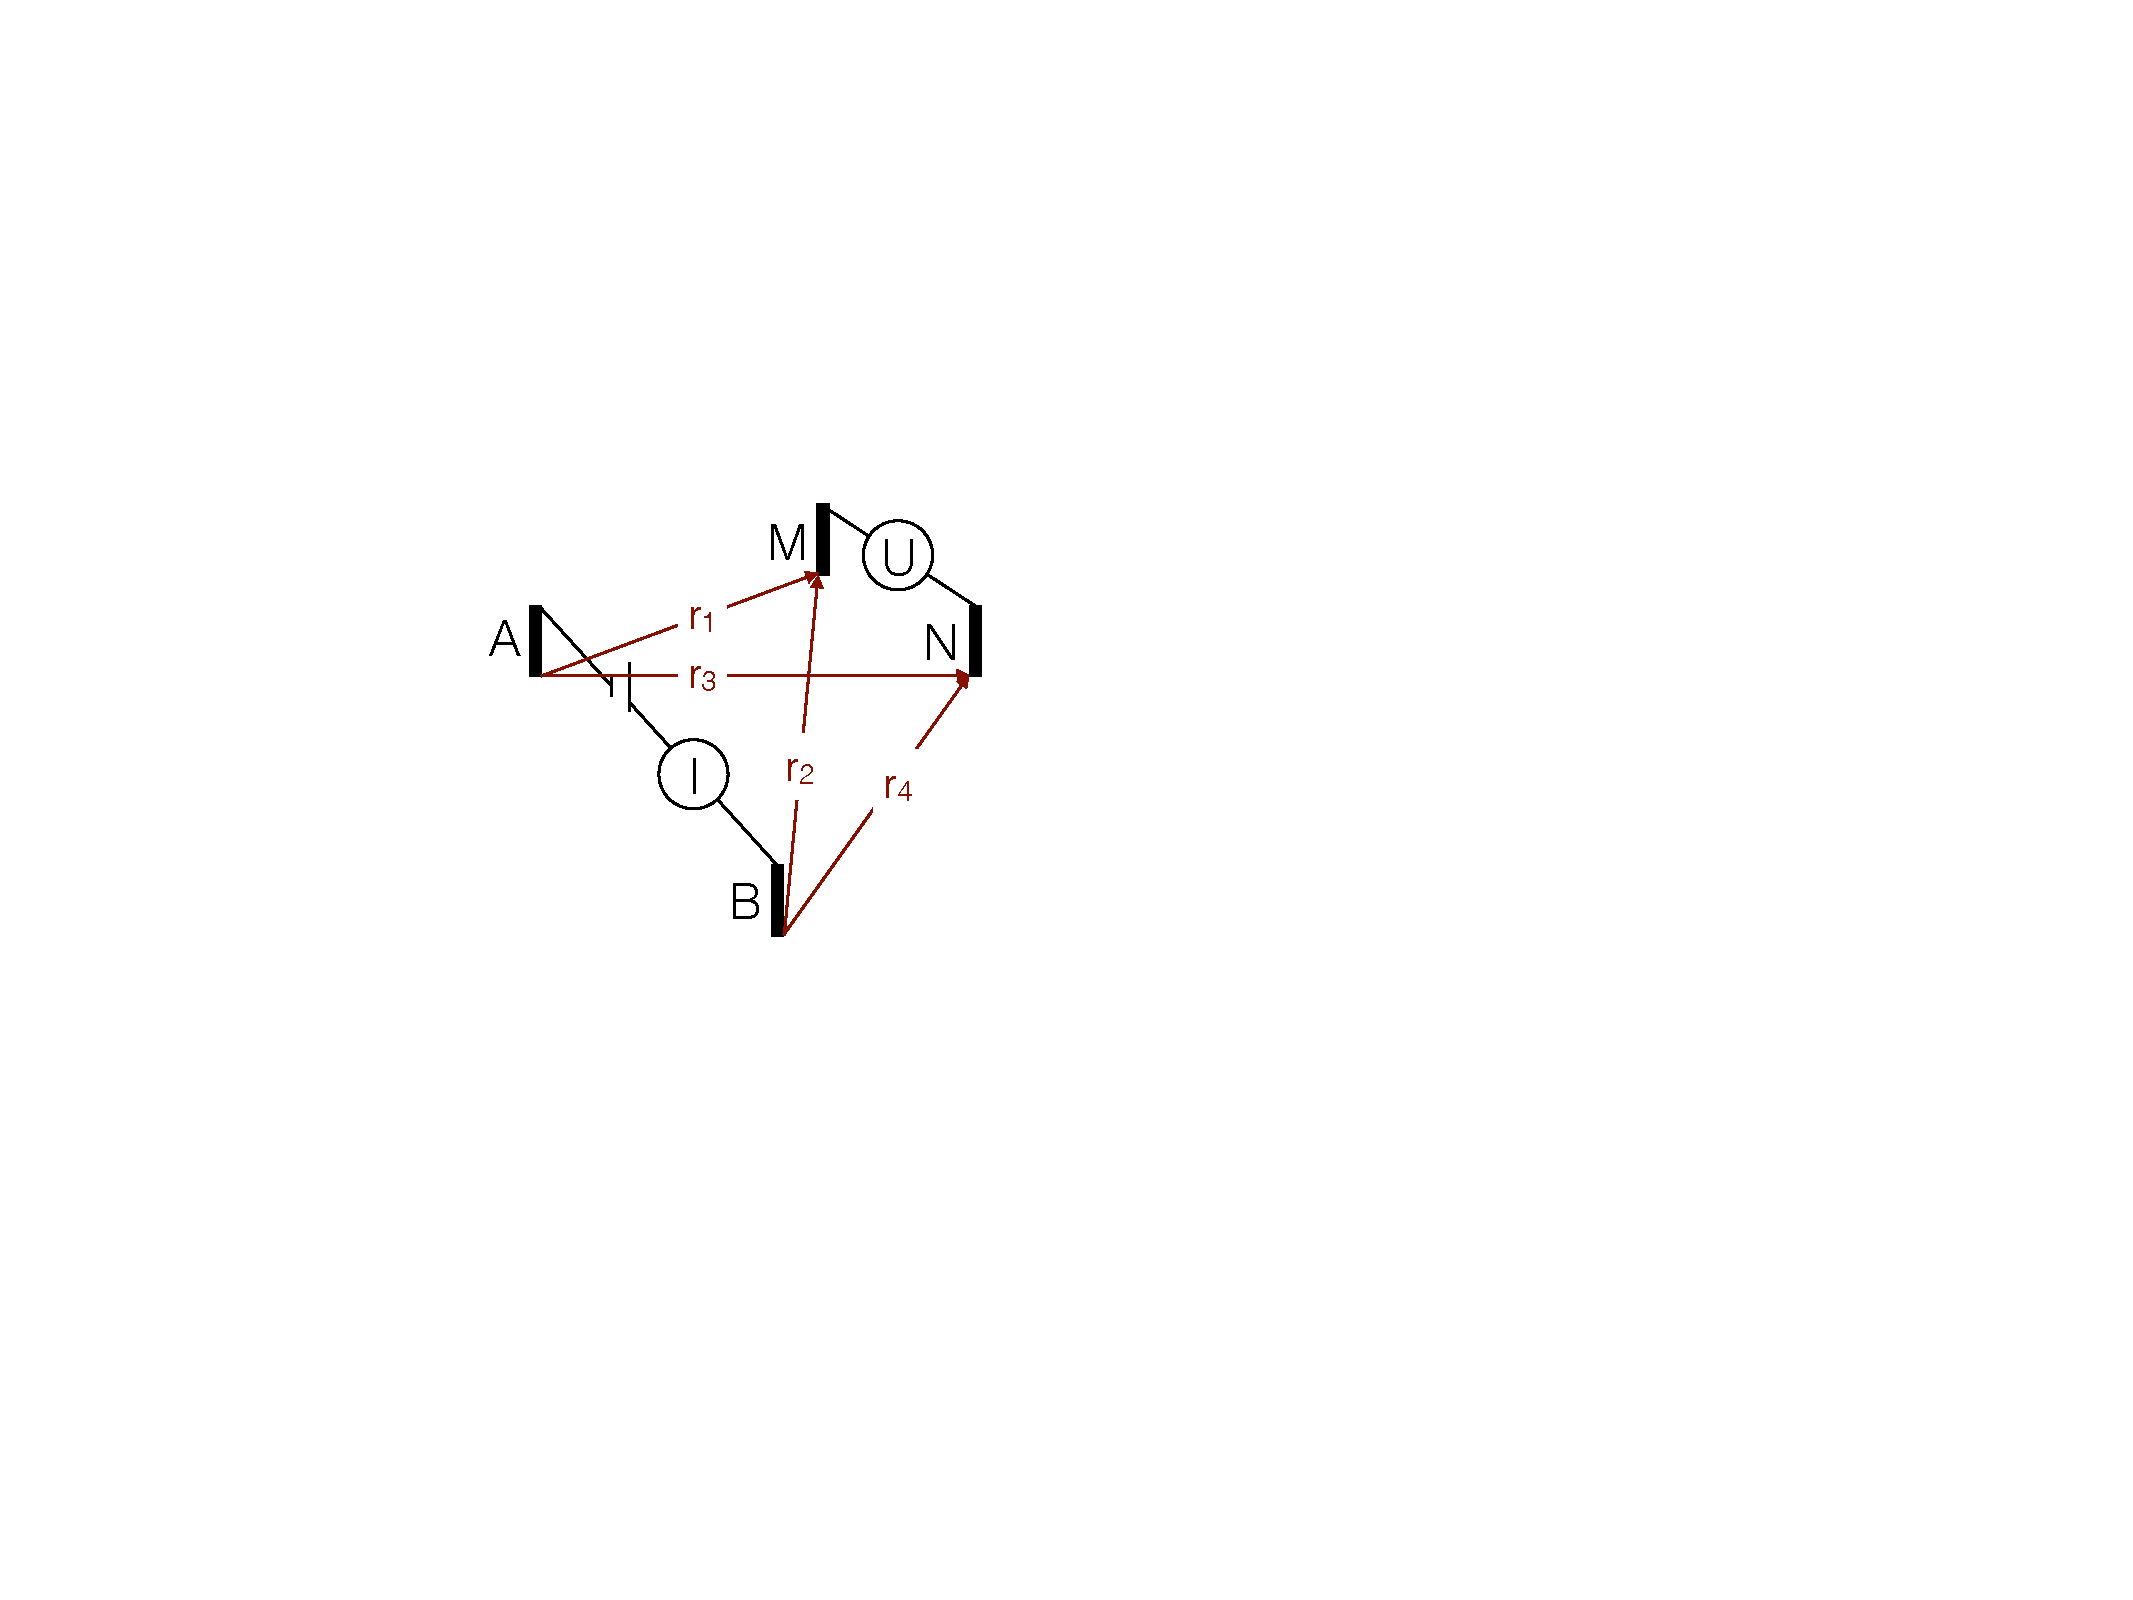
\includegraphics[scale = 0.8]{GeoelektrikBilder/beliebigeVierpunktanordnung}
\end{figure}



\subsection{Sondierung}
Ist eine Untersuchung der Struktur unter einem bestimmten Punkt vorgesehen, eignet sich die \textbf{Schlumberger-Anordnung}.
Bei dieser Messkonfiguration ist der Abstand zwischen den Elektroden A und B deutlich größer als der Abstand zwischen den Sonden M und N. Im Laufe der Messung wird der Abstand von A und B symmetrisch zu N und M immer weiter vergrößert, während N und M am selben Ort bleiben. Durch diese Art der Messung ergeben sich Informationen über den spezifischen Widerstand in immer größeren Tiefen.


\begin{figure}[H]
	\centering
	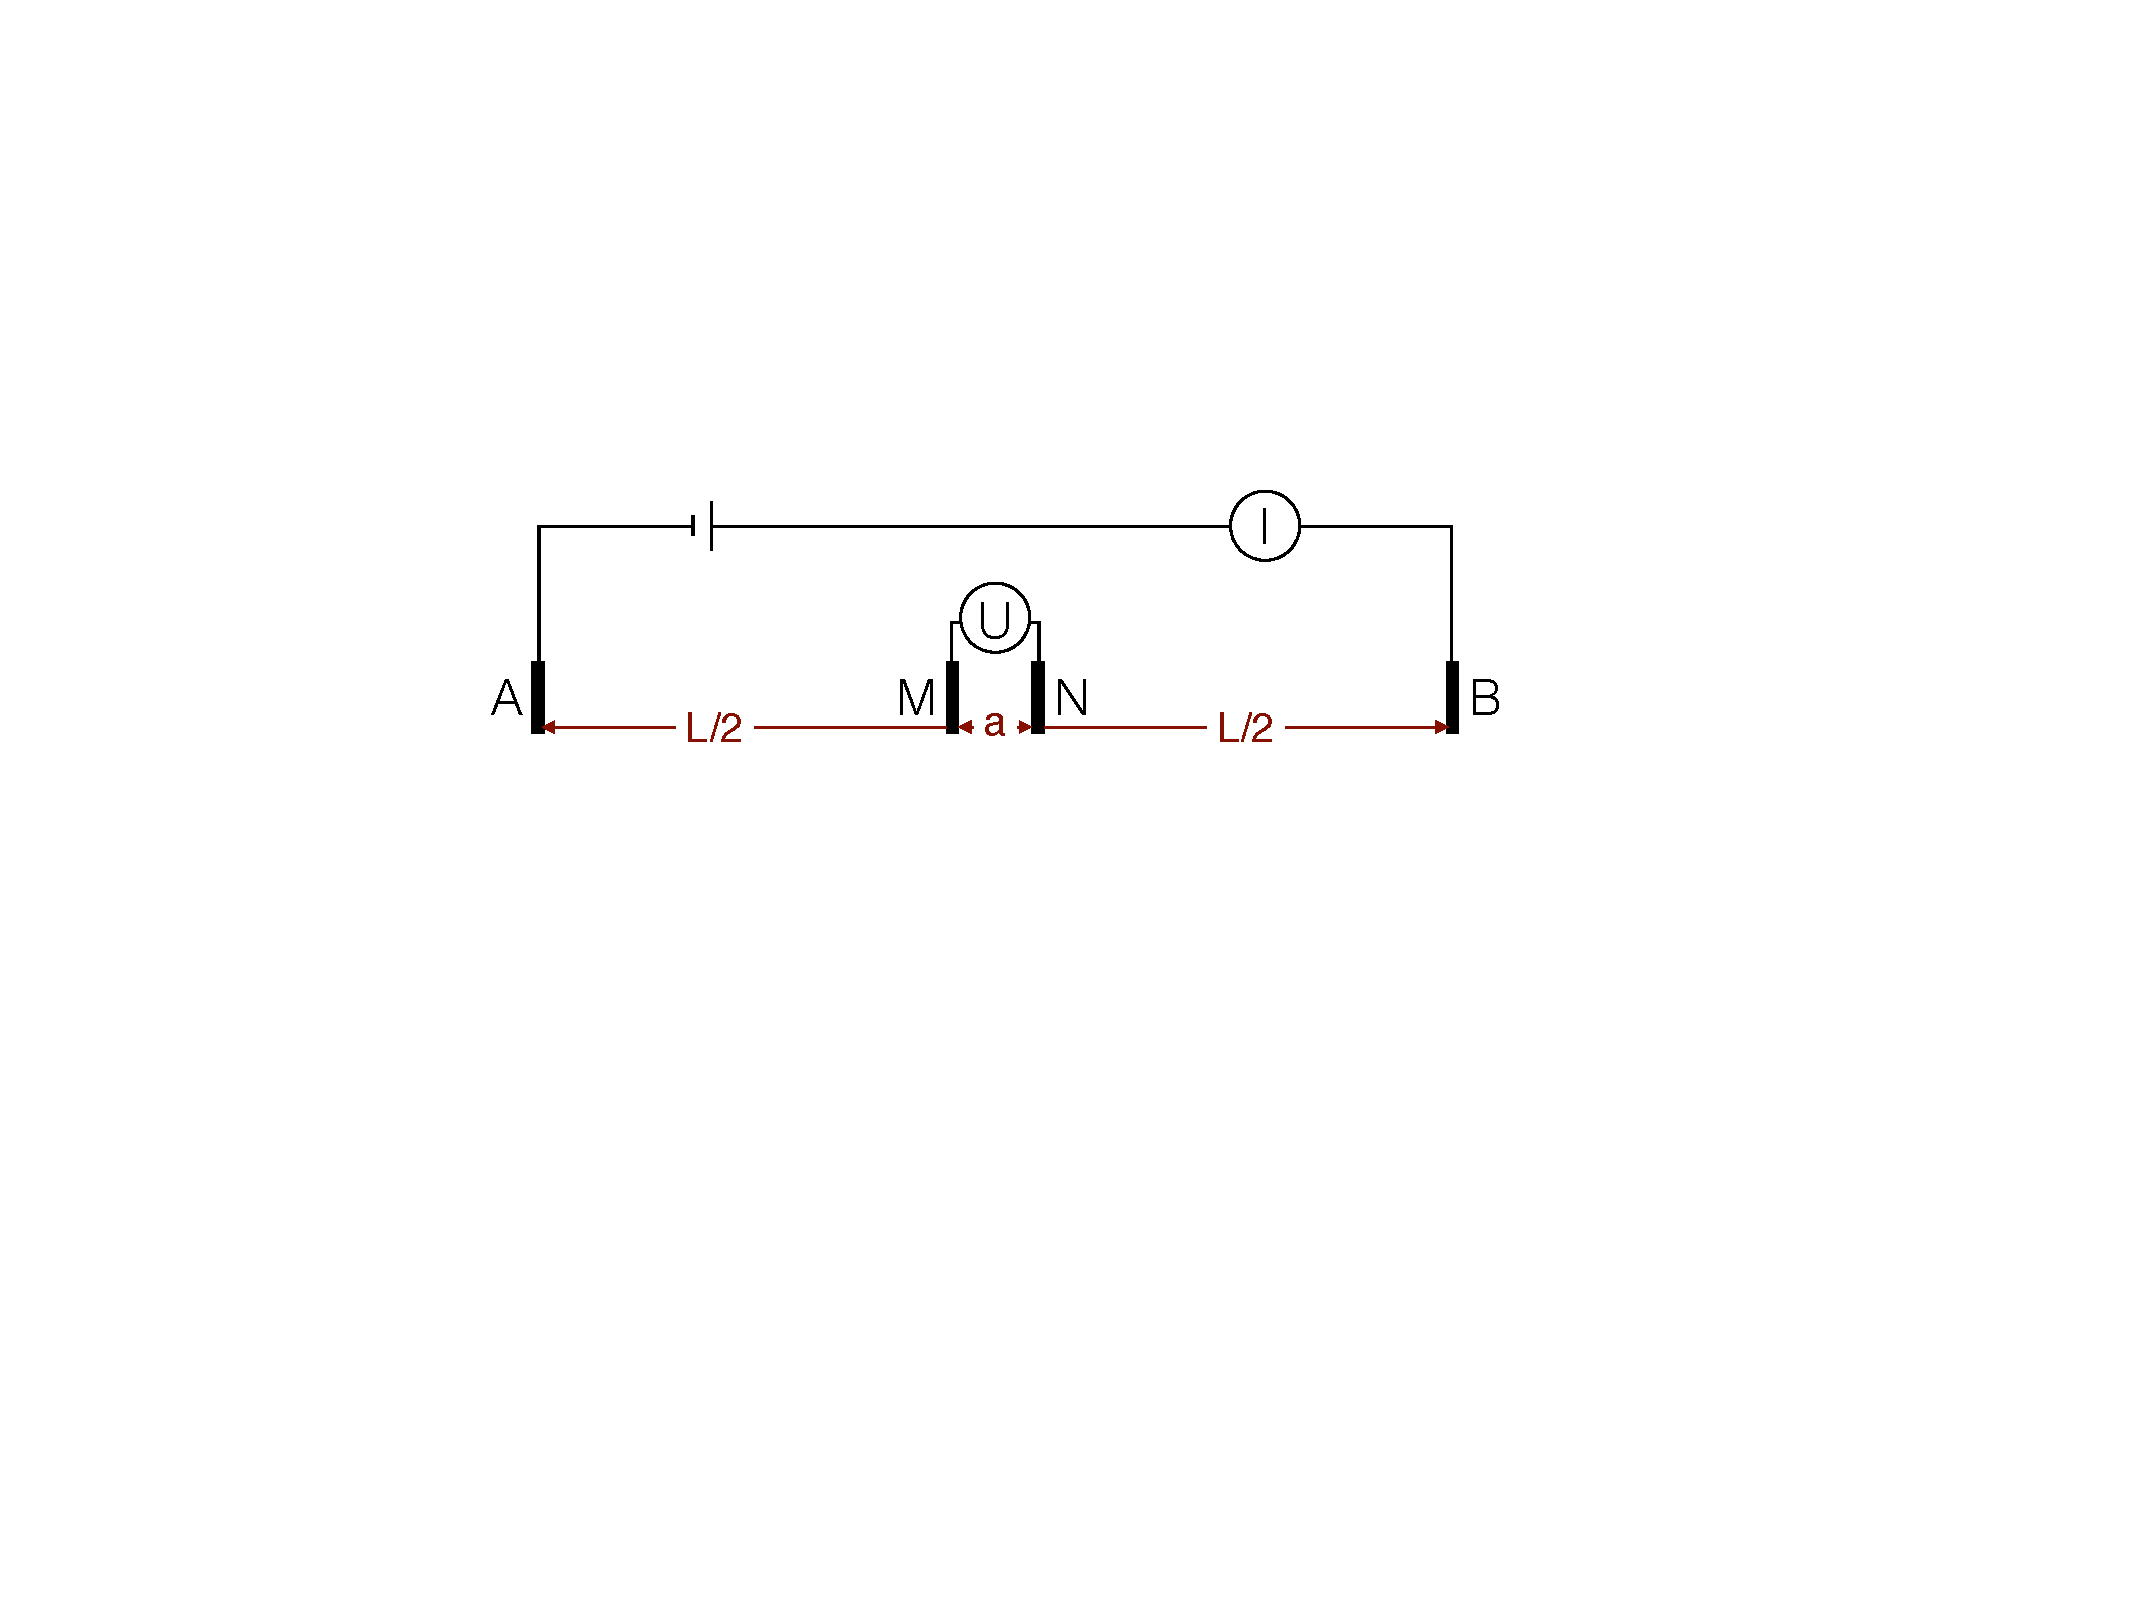
\includegraphics[width = \textwidth]{GeoelektrikBilder/SchlumbergerAnordnung}
\end{figure}


\subsection{Kartierung}
Von einer Kartierung spricht man dann, wenn die Struktur in einer bestimmten Tiefe flächenhaft untersucht werden soll. Hierfür findet die \textbf{Wenner-Anordnung} Verwendung. Im Vergleich zur Schlumberger-Anordnung ist hier der Abstand aller Elektroden und Sonden gleich. Im Laufe der Messung wird die gesamte Messauslage mit festem Abstand entlang des zu untersuchenden Profils bewegt. Der Elektrodenabstand entspricht etwa der Eindringtiefe.


\begin{figure}[H]
	\centering
	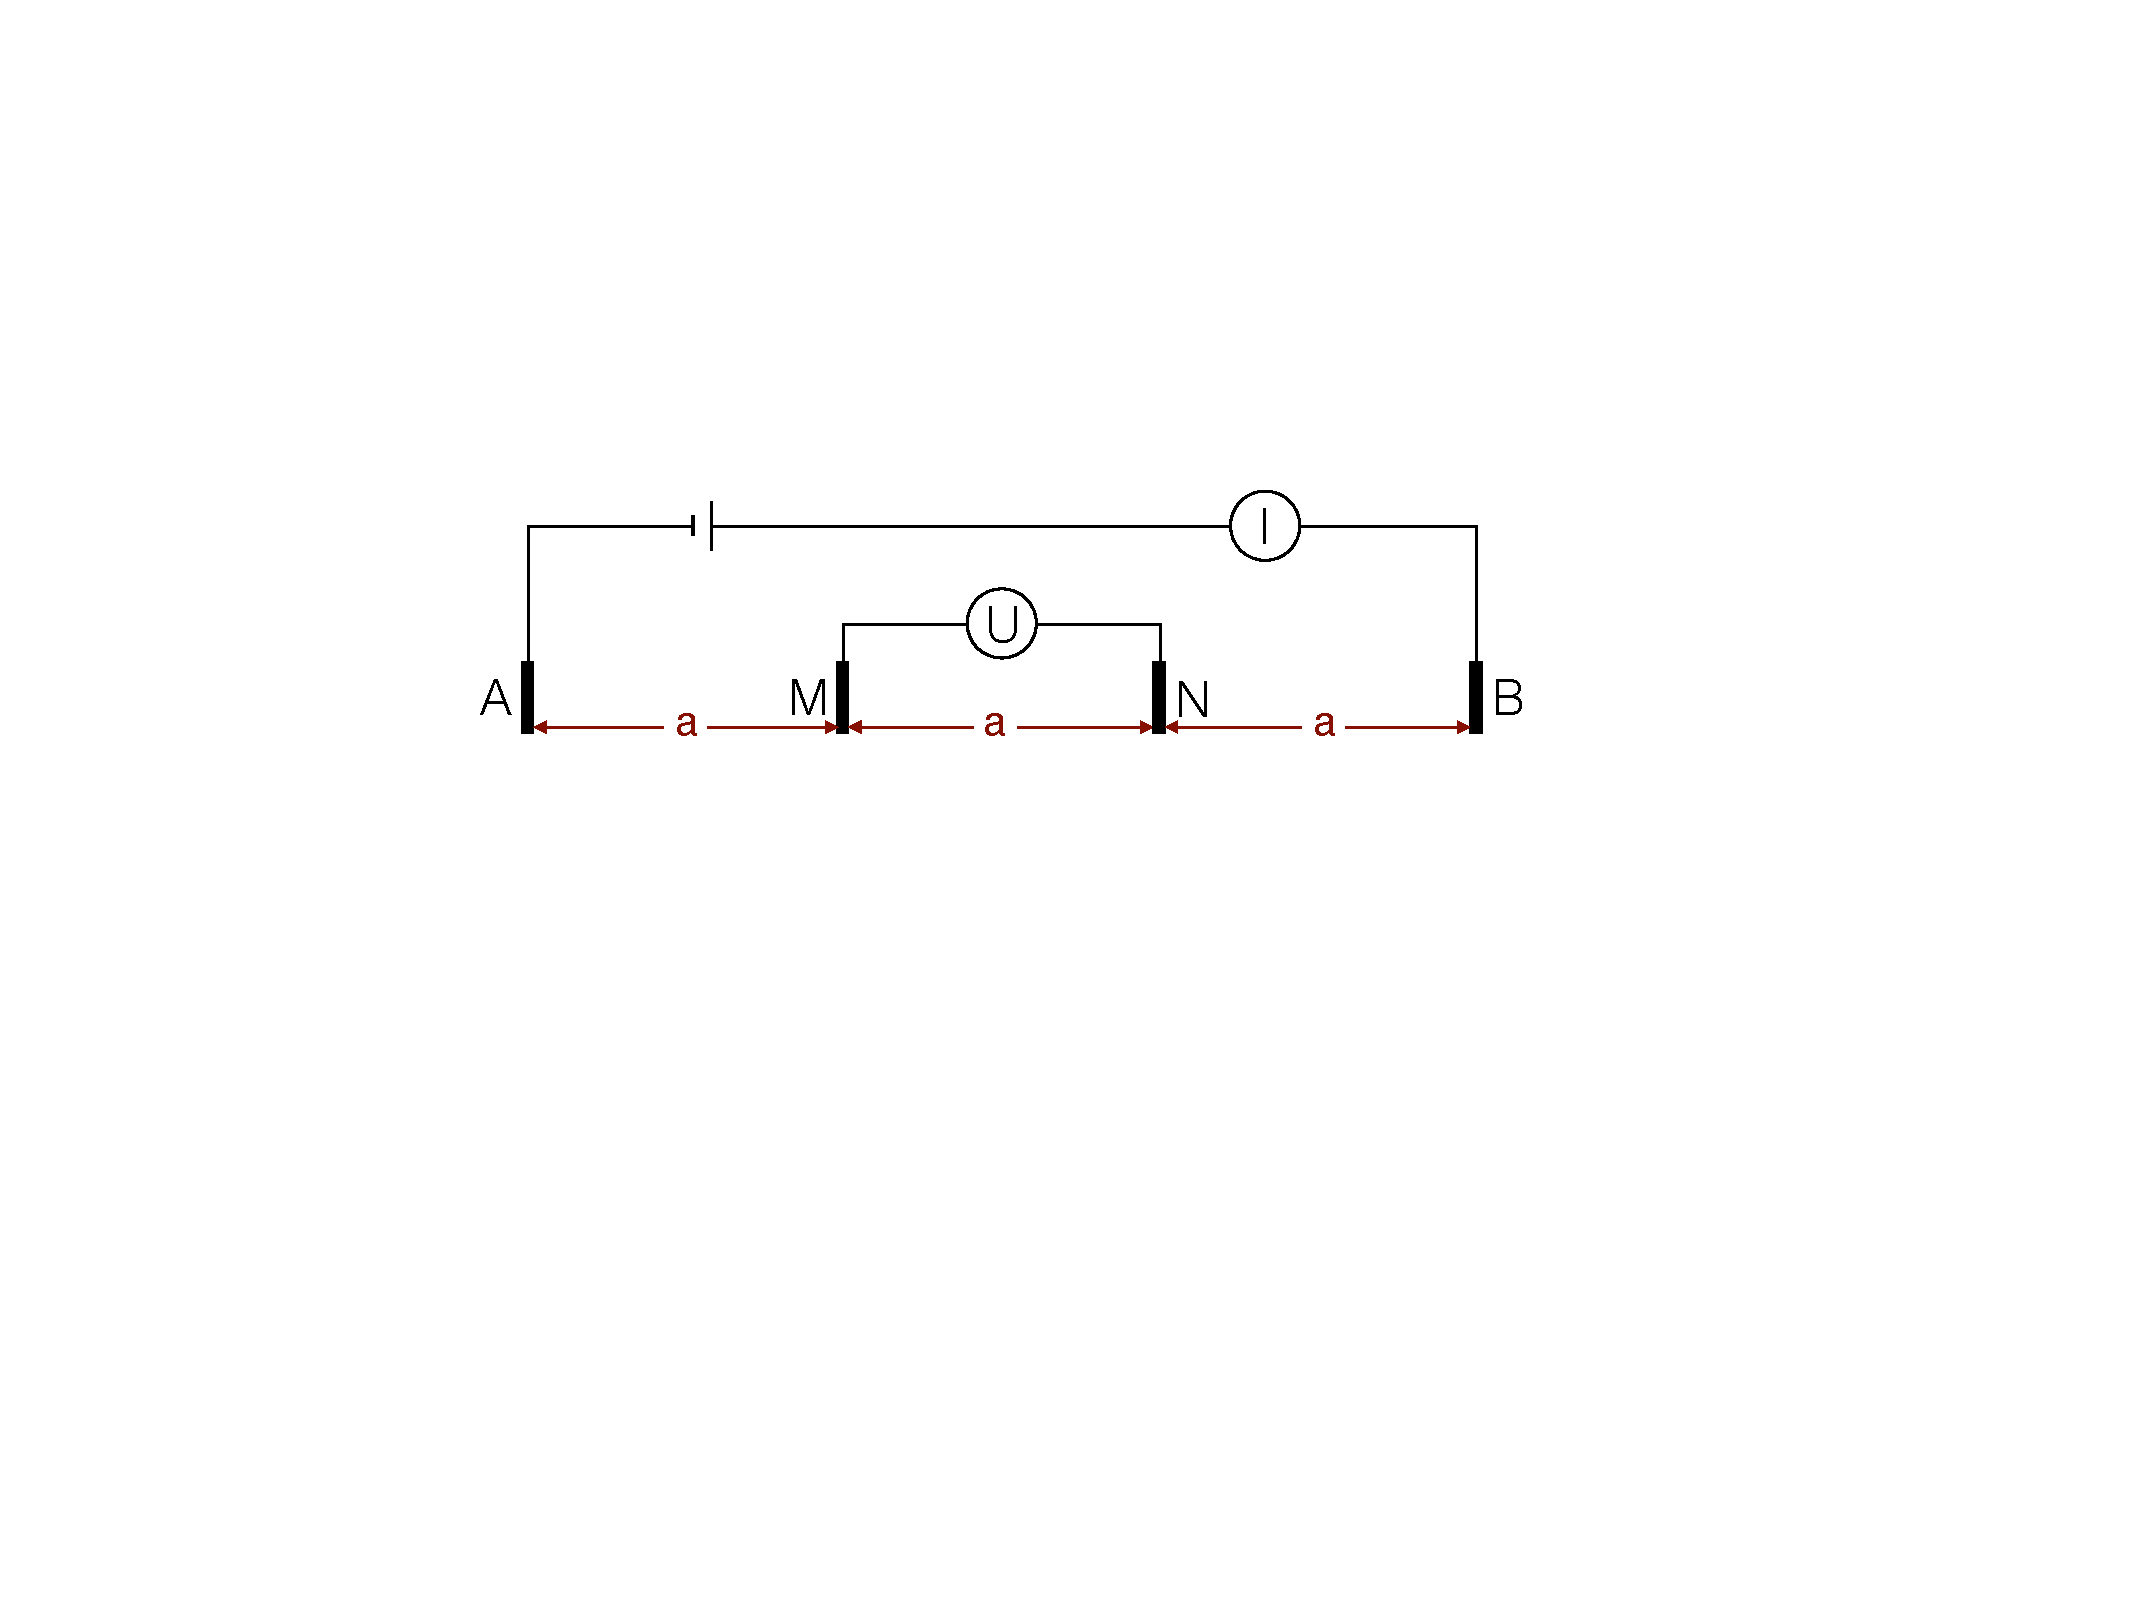
\includegraphics[width = \textwidth]{GeoelektrikBilder/WennerAnordnung}
\end{figure}



\subsection{Dipol-Dipol-Anordnung}
Diese Anordnung trennt Spannungsmessung und Stromzufuhr. Die Elektroden A und B zur Stromeinspeisung haben dabei den selben Abstand $a$ wie die Sonden N und M zur Spannungsmessung. Der Abstand dieser beiden Paare ist ein Vielfaches von $a$.

\begin{figure}[H]
	\centering
	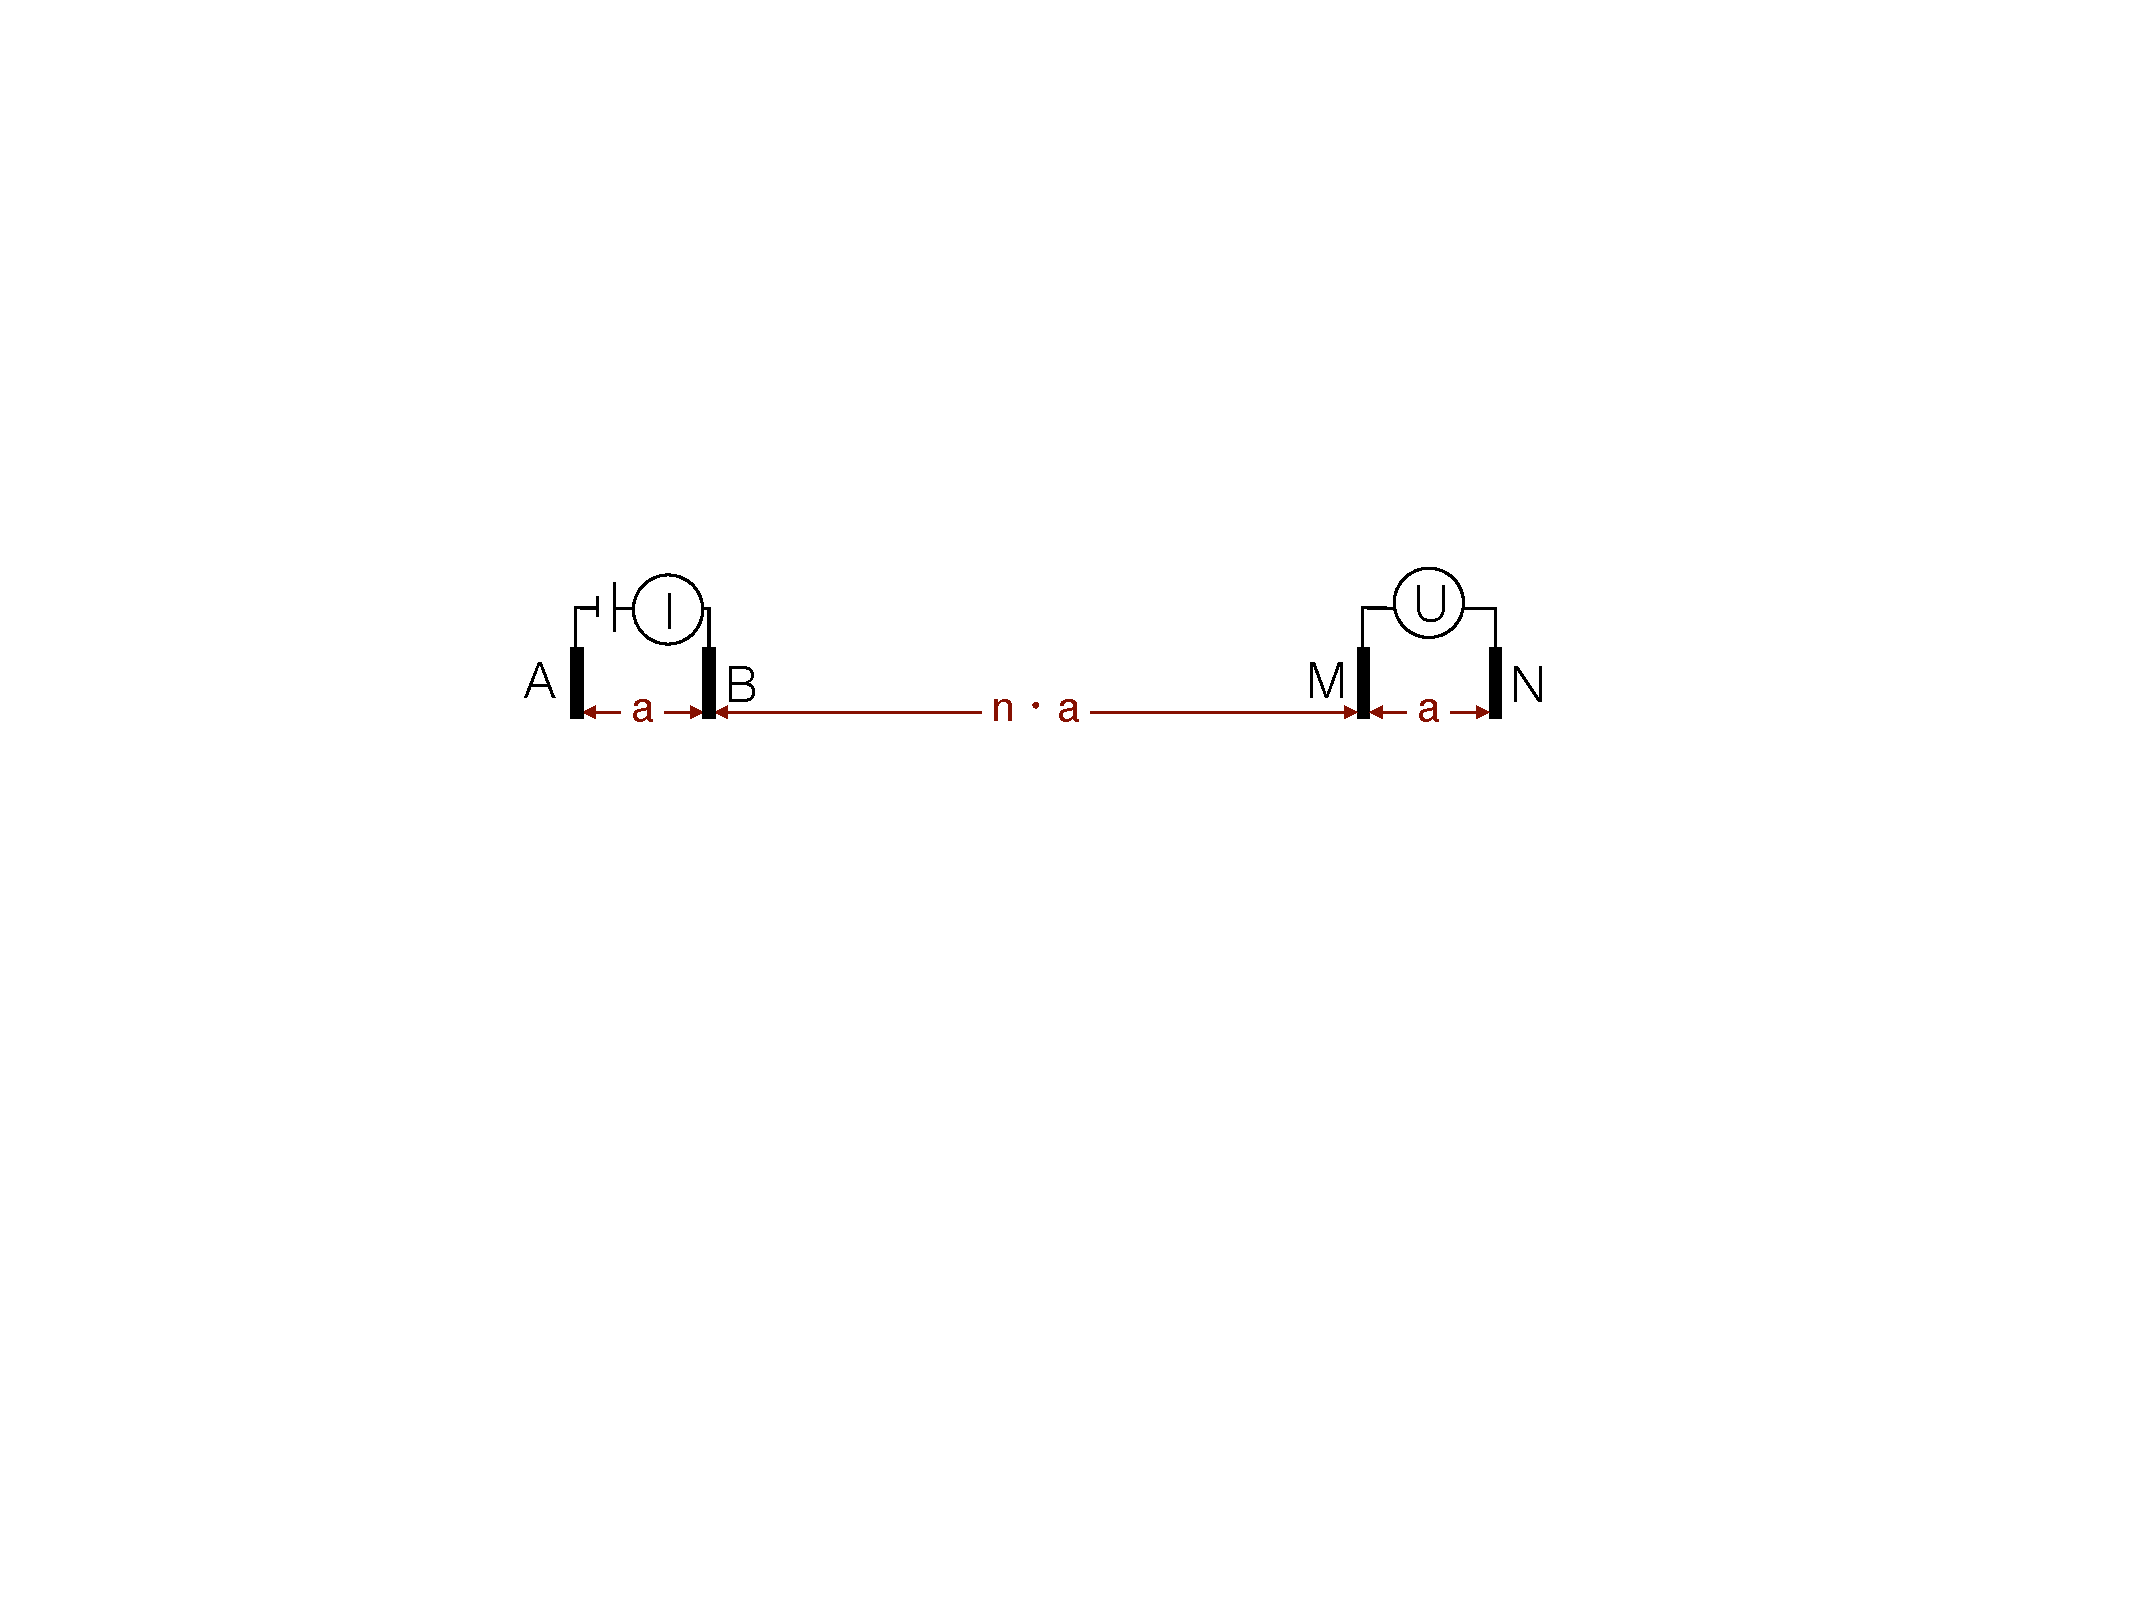
\includegraphics[width = \textwidth]{GeoelektrikBilder/DipolDipolAnordnung}
\end{figure}


\section{Auswertung}
Um Rückschlüsse auf die Beschaffenheit des Untergrundes ziehen zu können, muss der scheinbare spezifische Widerstand $\rho_{\text{s}}$ berechnet werden. 
Bei Gleichstromverfahren ist das relativ einfach. Der scheinbare spezifische Widerstand berechnet sich zu \begin{equation*}
	\rho_{\text{s}} = R \cdot K = \frac{U}{I} \cdot K
\end{equation*}

$K$ bezeichnet hierbei den Geometriefaktor der verwendeten Anordnung.

Verändert sich der scheinbare spezifische Widerstand im Laufe einer Messung kaum oder nicht, spricht man vom Medium des Untergrundes als homogenen Halbraum. 

Für die Auswertung des spezifischen Widerstandes gibt es gewissen Anhaltspunkte. In Mineralen ist der spezifische Widerstand groß und in Metallen, Erzen oder Graphit klein. \\
Eine Diskontinuität im Untergrund kenntzeichnet sich durch eine deutliche Veränderung des spezifischen Widerstandes. Solche signifikanten Änderungen werden beispielsweise durch Wasser, Salze oder Metalle und Erze hervorgerufen. Um ein Gefühl für die Größenunterschiede zu bekommen, seien nun noch ein paar Literaturwerte genannt. 

\begin{tabular}{ll}
	\textbf{Gestein} & \textbf{spezifischer Widerstand [$\Omega$m]} \\
	Sand (trocken) & $10^5$ \\
	Sand (wassergesättigt) & 1000 -- $10^4$ \\
	Granit & 300 - $3 \cdot 10^4$ \\
	Kalkstein & 100 -- 7000 \\
	Lehme & 3 -- 300 \\
	Ton (trocken) & 30 -- 1000 \\
	Ton (nass) & 1-30
\end{tabular}  

\subsection{Geometriefaktor}
Dieser Faktor ist wichtig, da sich der scheinbare spezifische Widerstand je nach verwendeter Anordnung ändert. Ohne Herleitung seien hier die Geometriefaktoren der vier präsentierten Messkonfigurationen genannt:

\subsubsection{beliebige Vierpunktanordnung}

\begin{figure}[H]
	\begin{subfigure}[m]{0.5\textwidth}
	\centering
		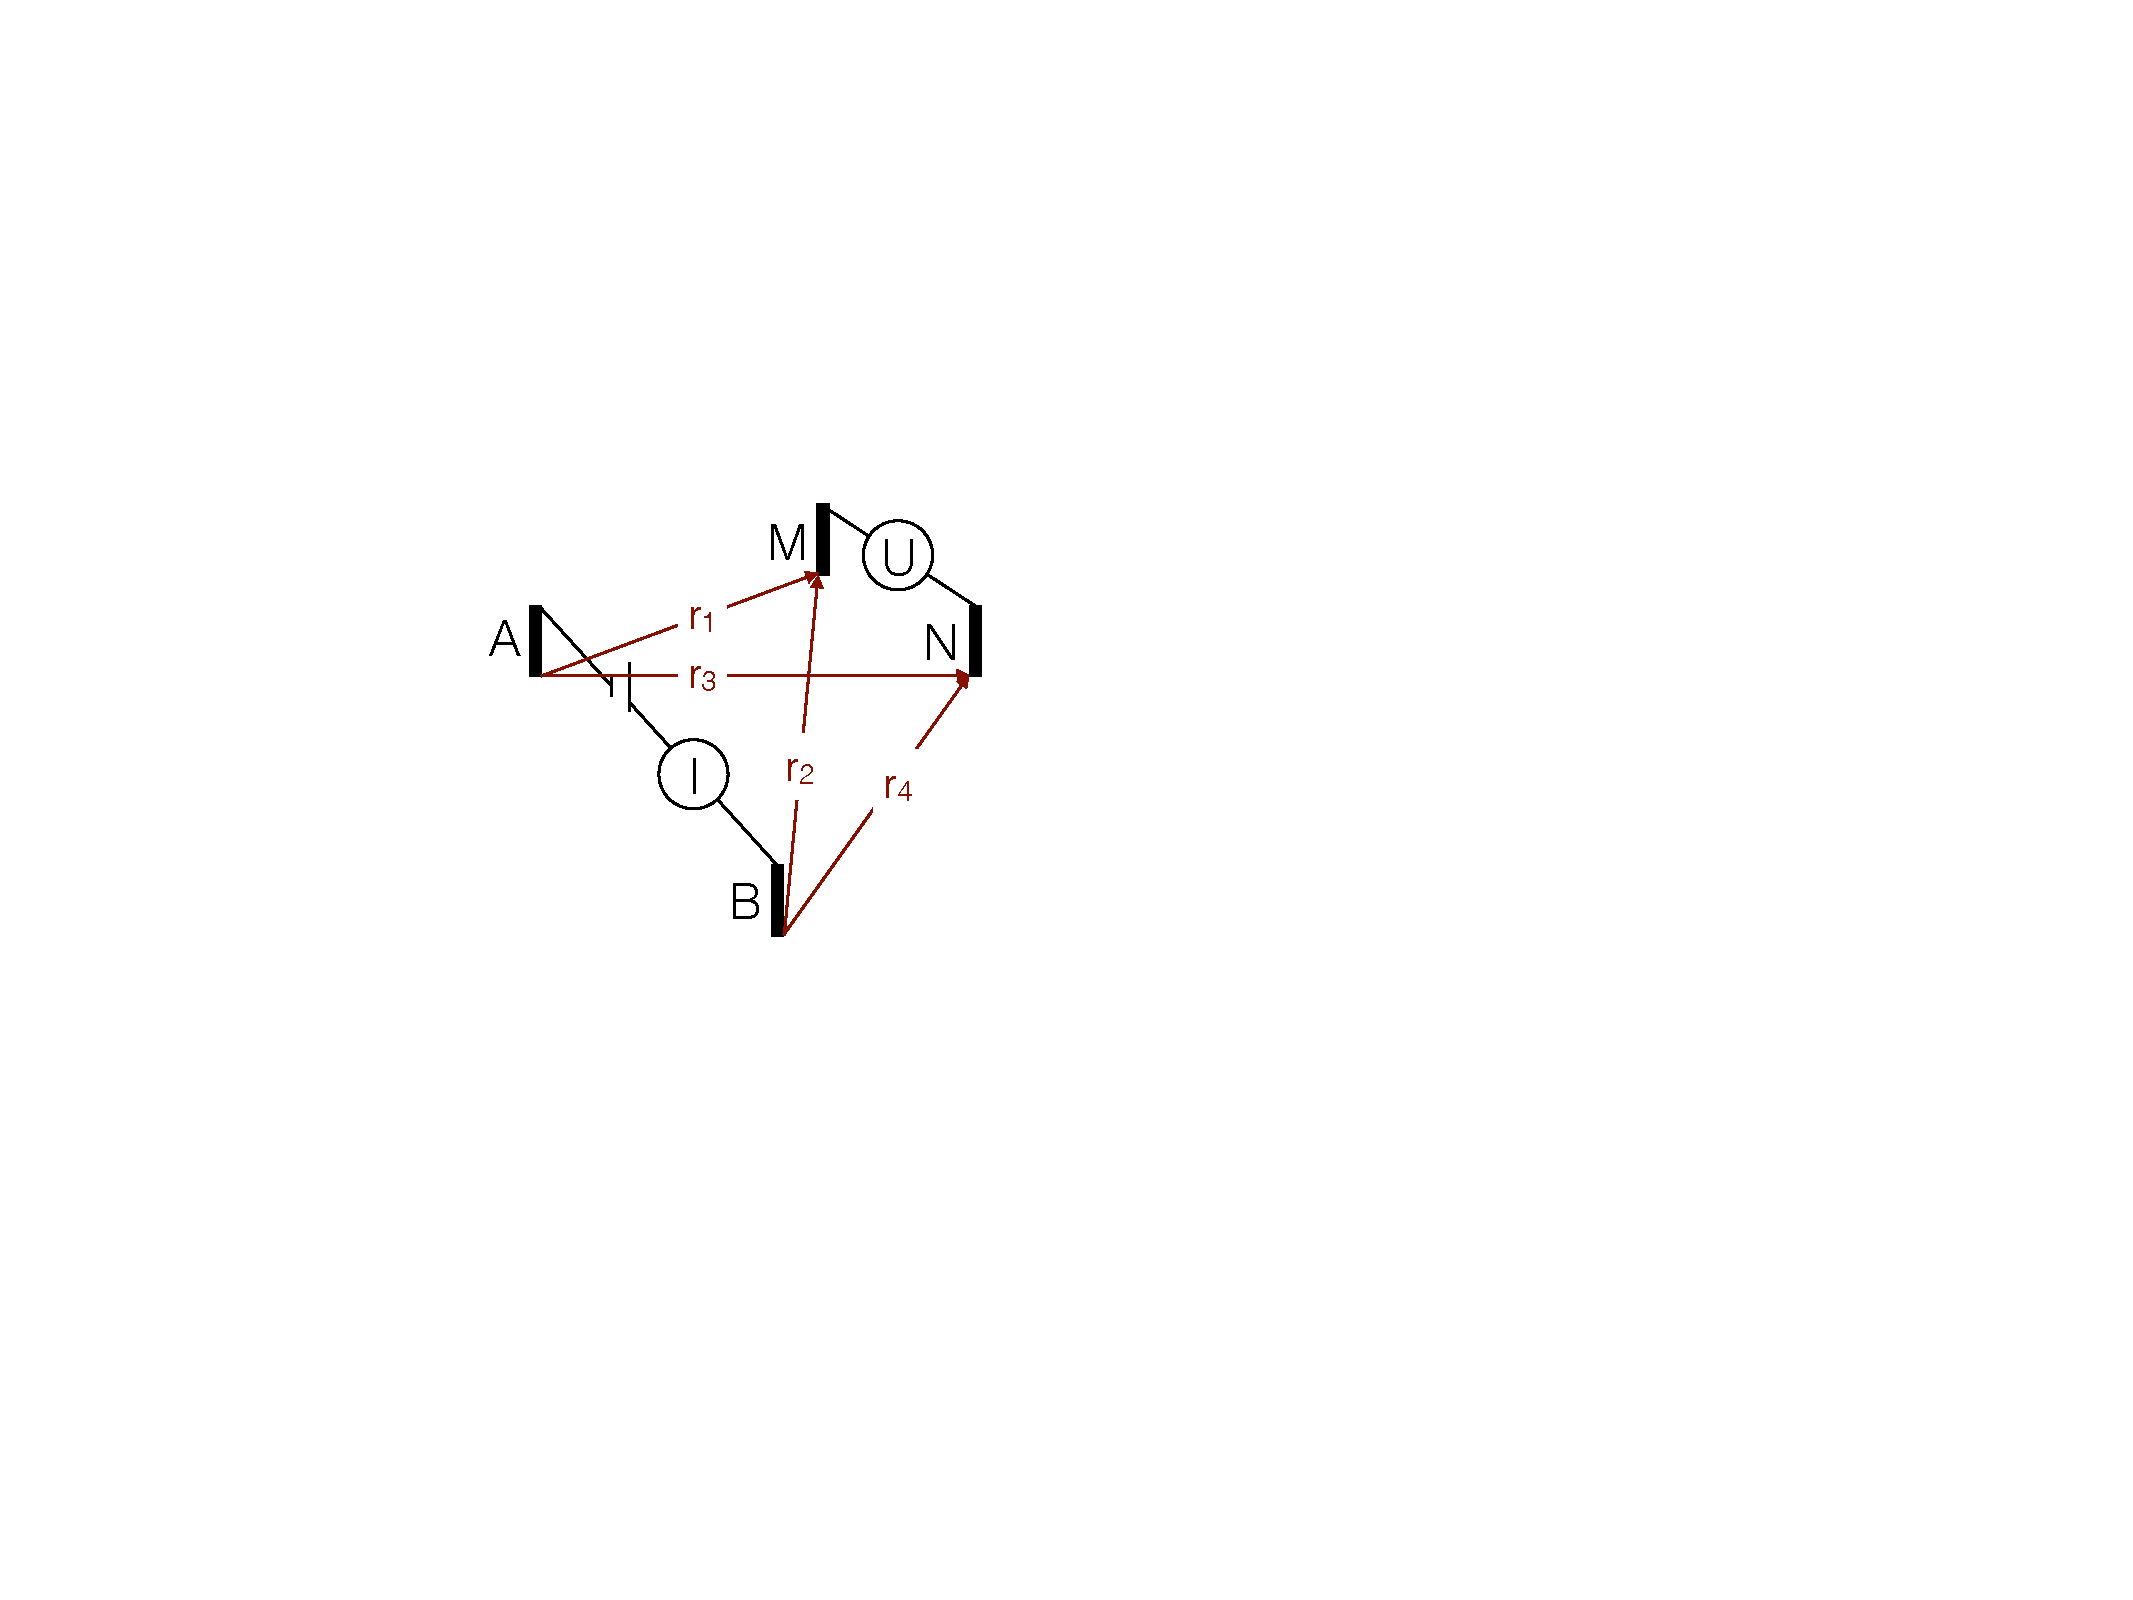
\includegraphics[scale = 0.5]{GeoelektrikBilder/beliebigeVierpunktanordnung}
	\end{subfigure}
	\begin{subfigure}[m]{0.5\textwidth}
		\begin{equation*}
			K = \frac{2 \pi}{\left( \frac{1}{r_1} - \frac{1}{r_2} \right) - \left( \frac{1}{r_3} - \frac{1}{r_4} \right)}
		\end{equation*}
	\end{subfigure}
\end{figure}


\subsubsection{Schlumberger-Anordnung}

\begin{figure}[H]
	\begin{subfigure}[m]{0.5\textwidth}
	\centering
		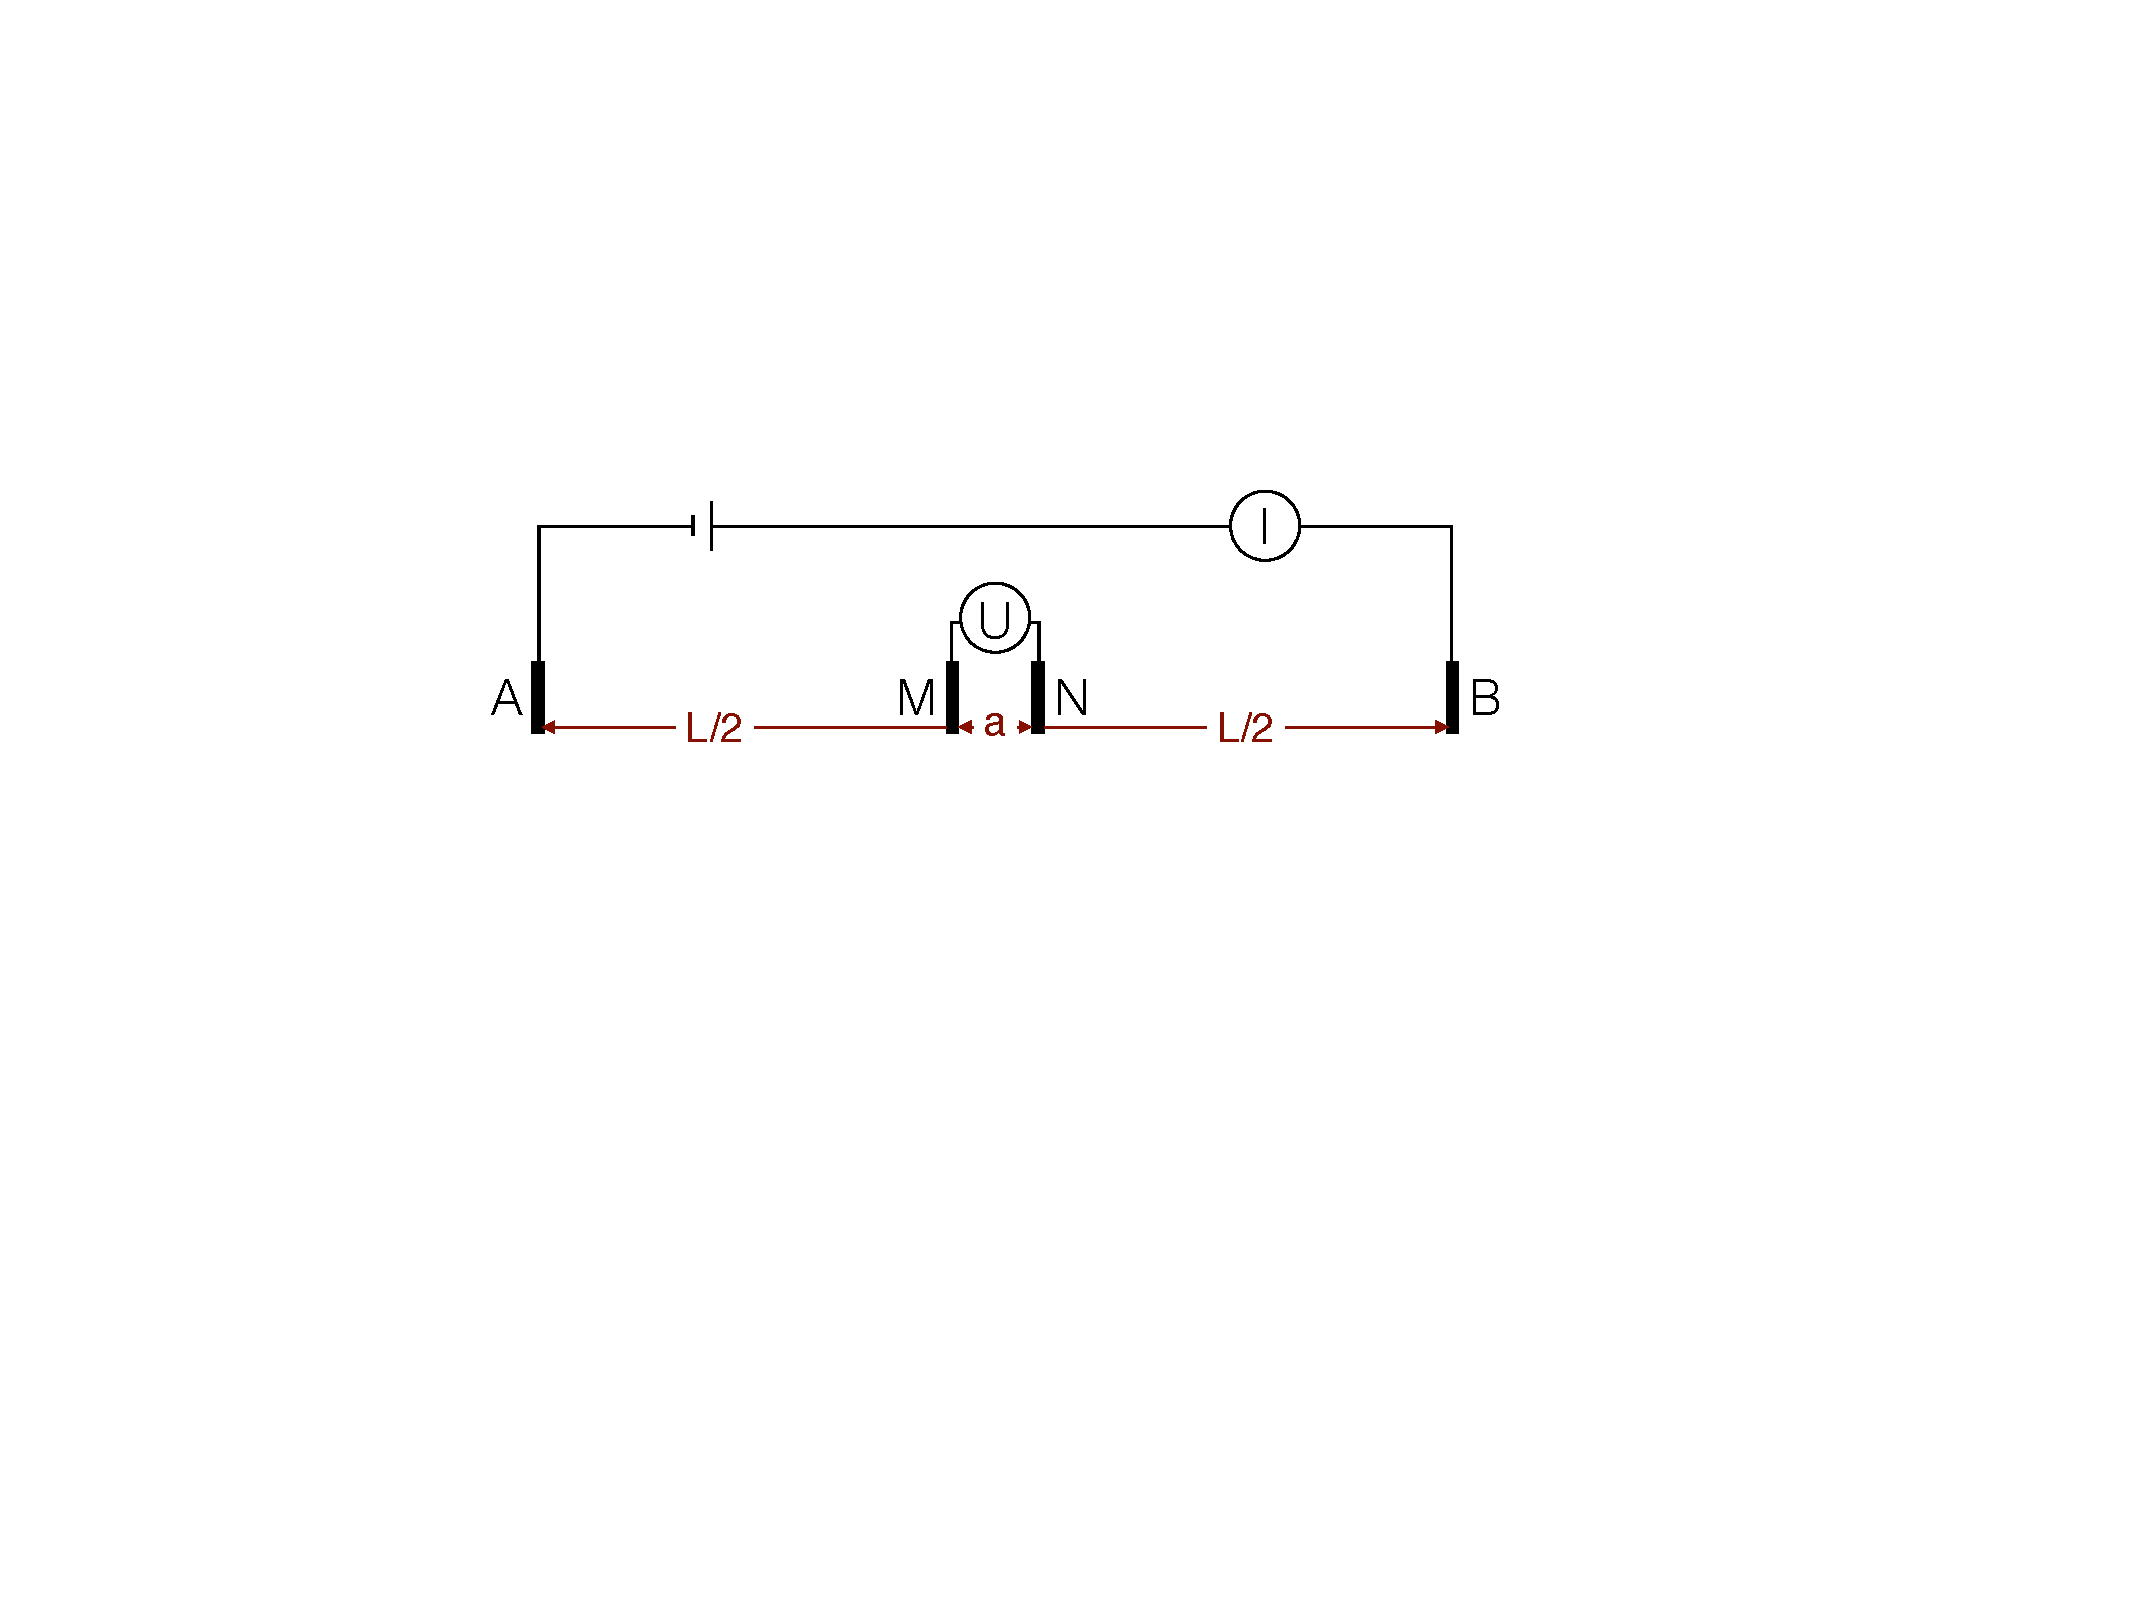
\includegraphics[scale = 0.4]{GeoelektrikBilder/SchlumbergerAnordnung}
	\end{subfigure}
	\begin{subfigure}[m]{0.5\textwidth}
		\begin{equation*}
			K = \frac{\pi}{a} \cdot \left( \frac{L}{2} \right)^2
		\end{equation*}
	\end{subfigure}
\end{figure}


\subsubsection{Wenner-Anordnung}

\begin{figure}[H]
	\begin{subfigure}[m]{0.5\textwidth}
	\centering
		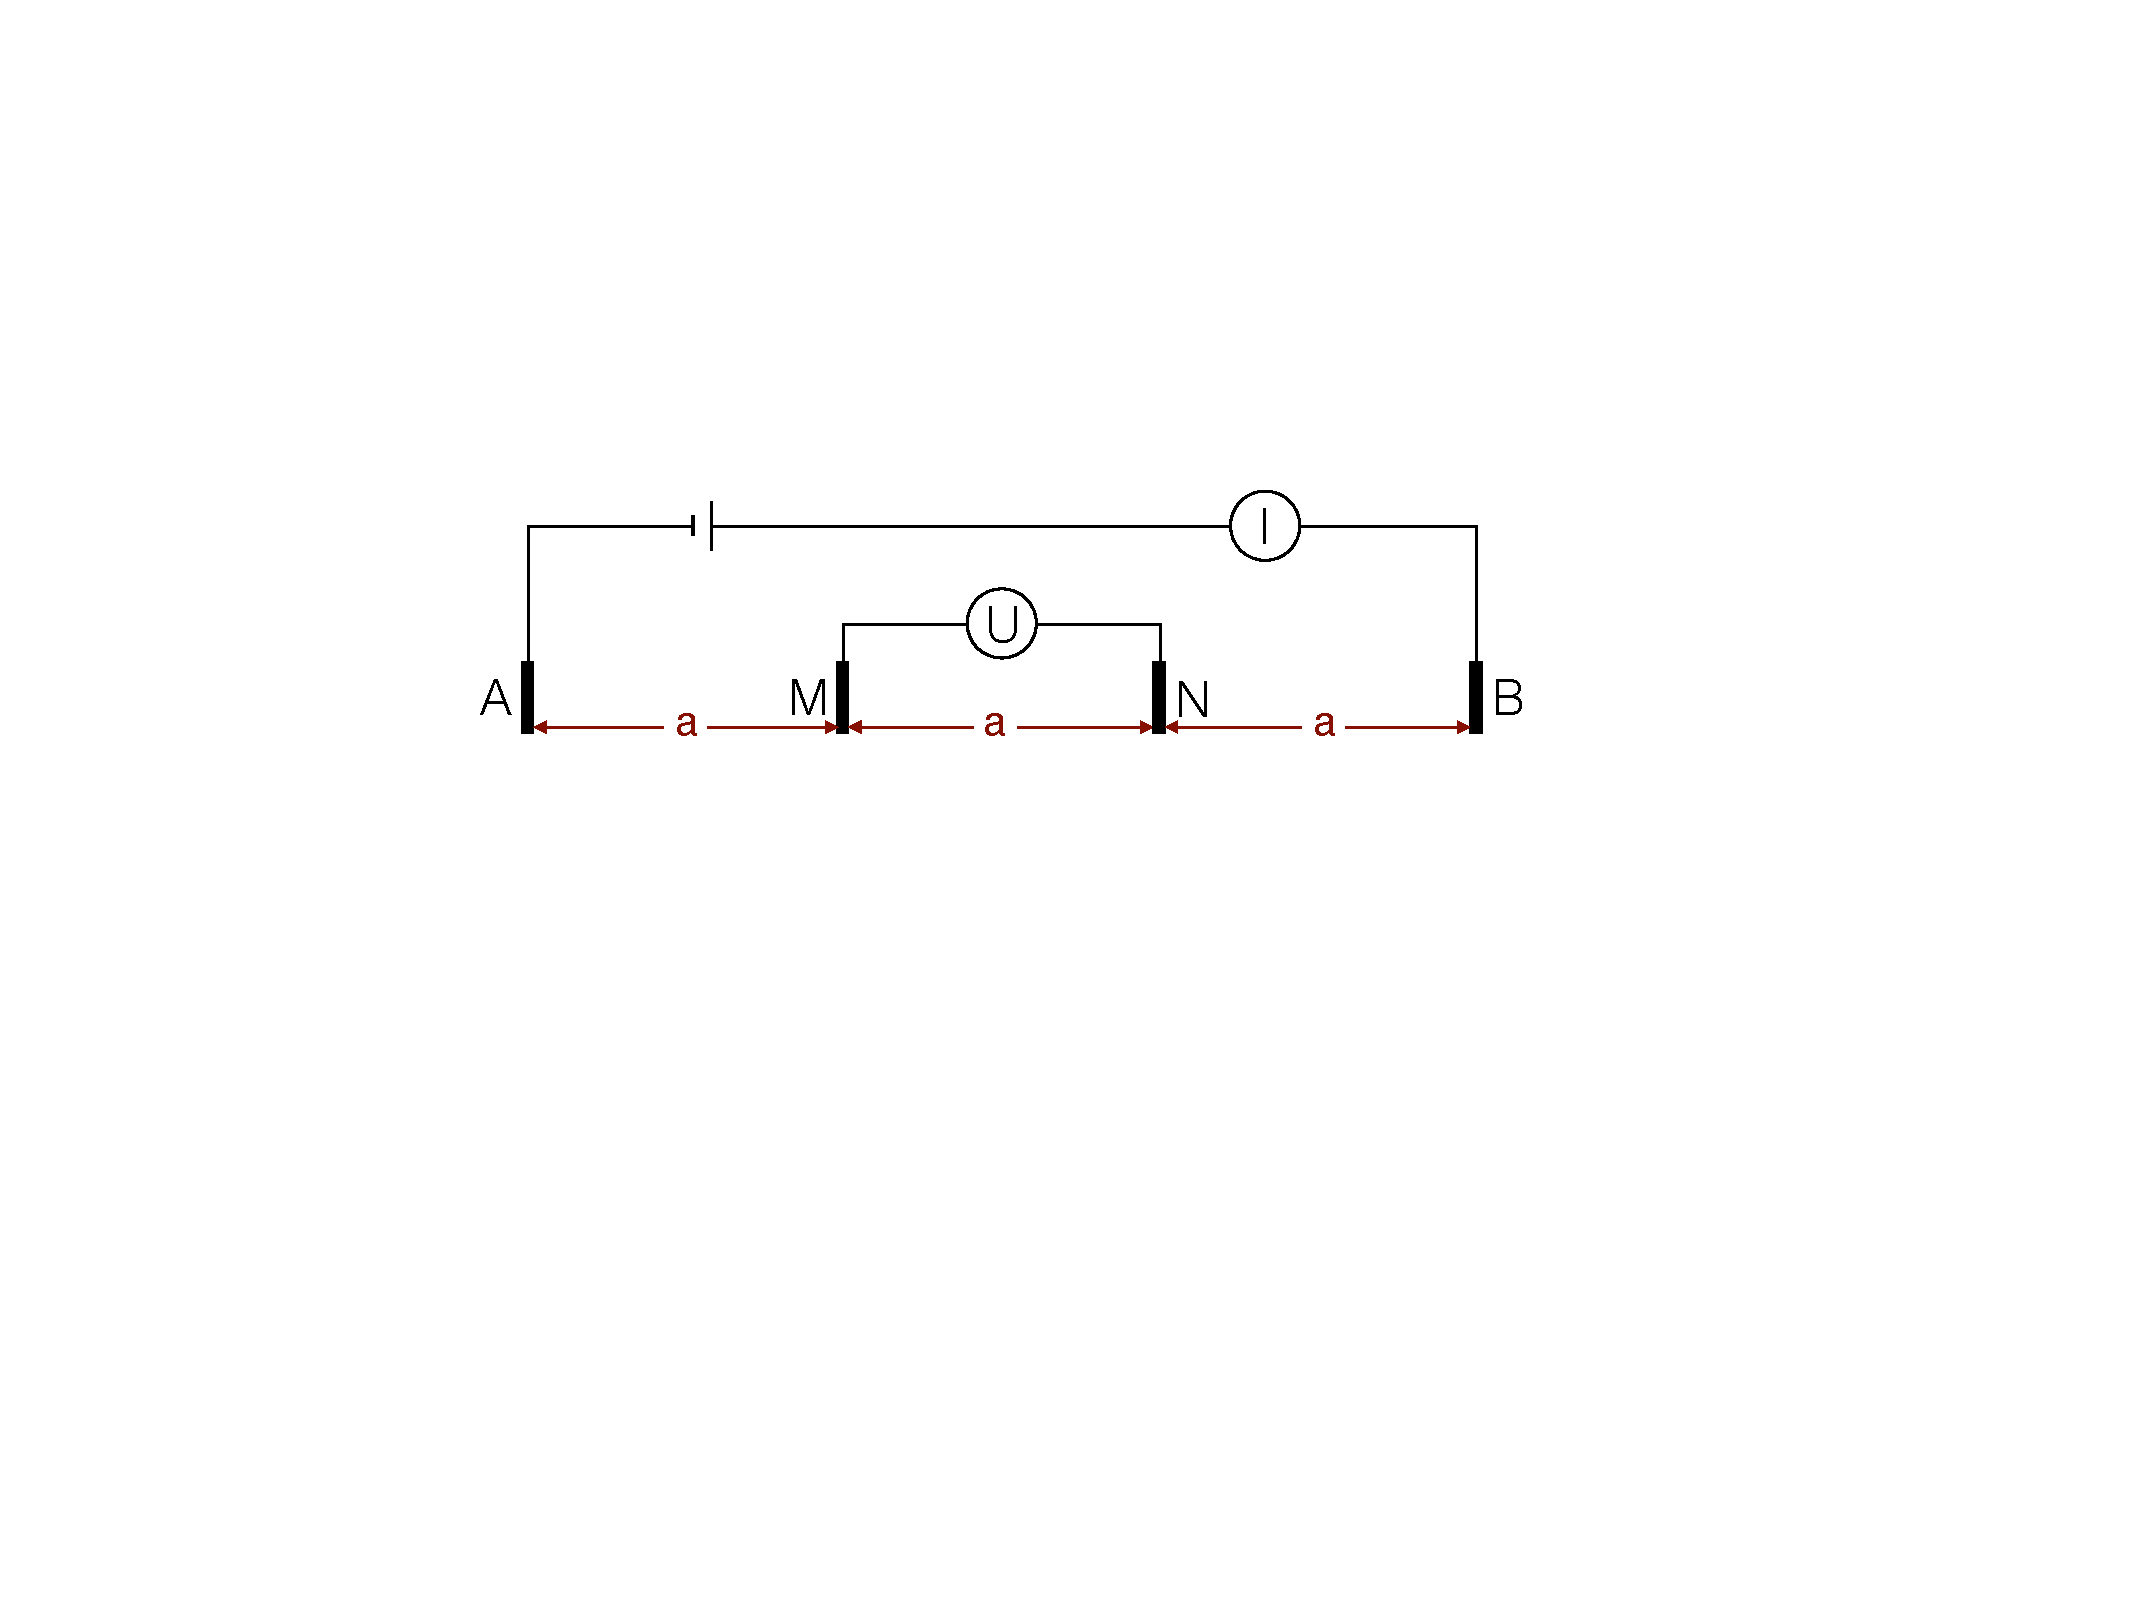
\includegraphics[scale = 0.4]{GeoelektrikBilder/WennerAnordnung}
	\end{subfigure}
	\begin{subfigure}[m]{0.5\textwidth}
		\begin{equation*}
				K = 2 \pi \cdot a
		\end{equation*}
	\end{subfigure}
\end{figure}



\subsubsection{Dipol-Dipol-Anordnung}

\begin{figure}[H]
	\begin{subfigure}[m]{0.5\textwidth}
	\centering
		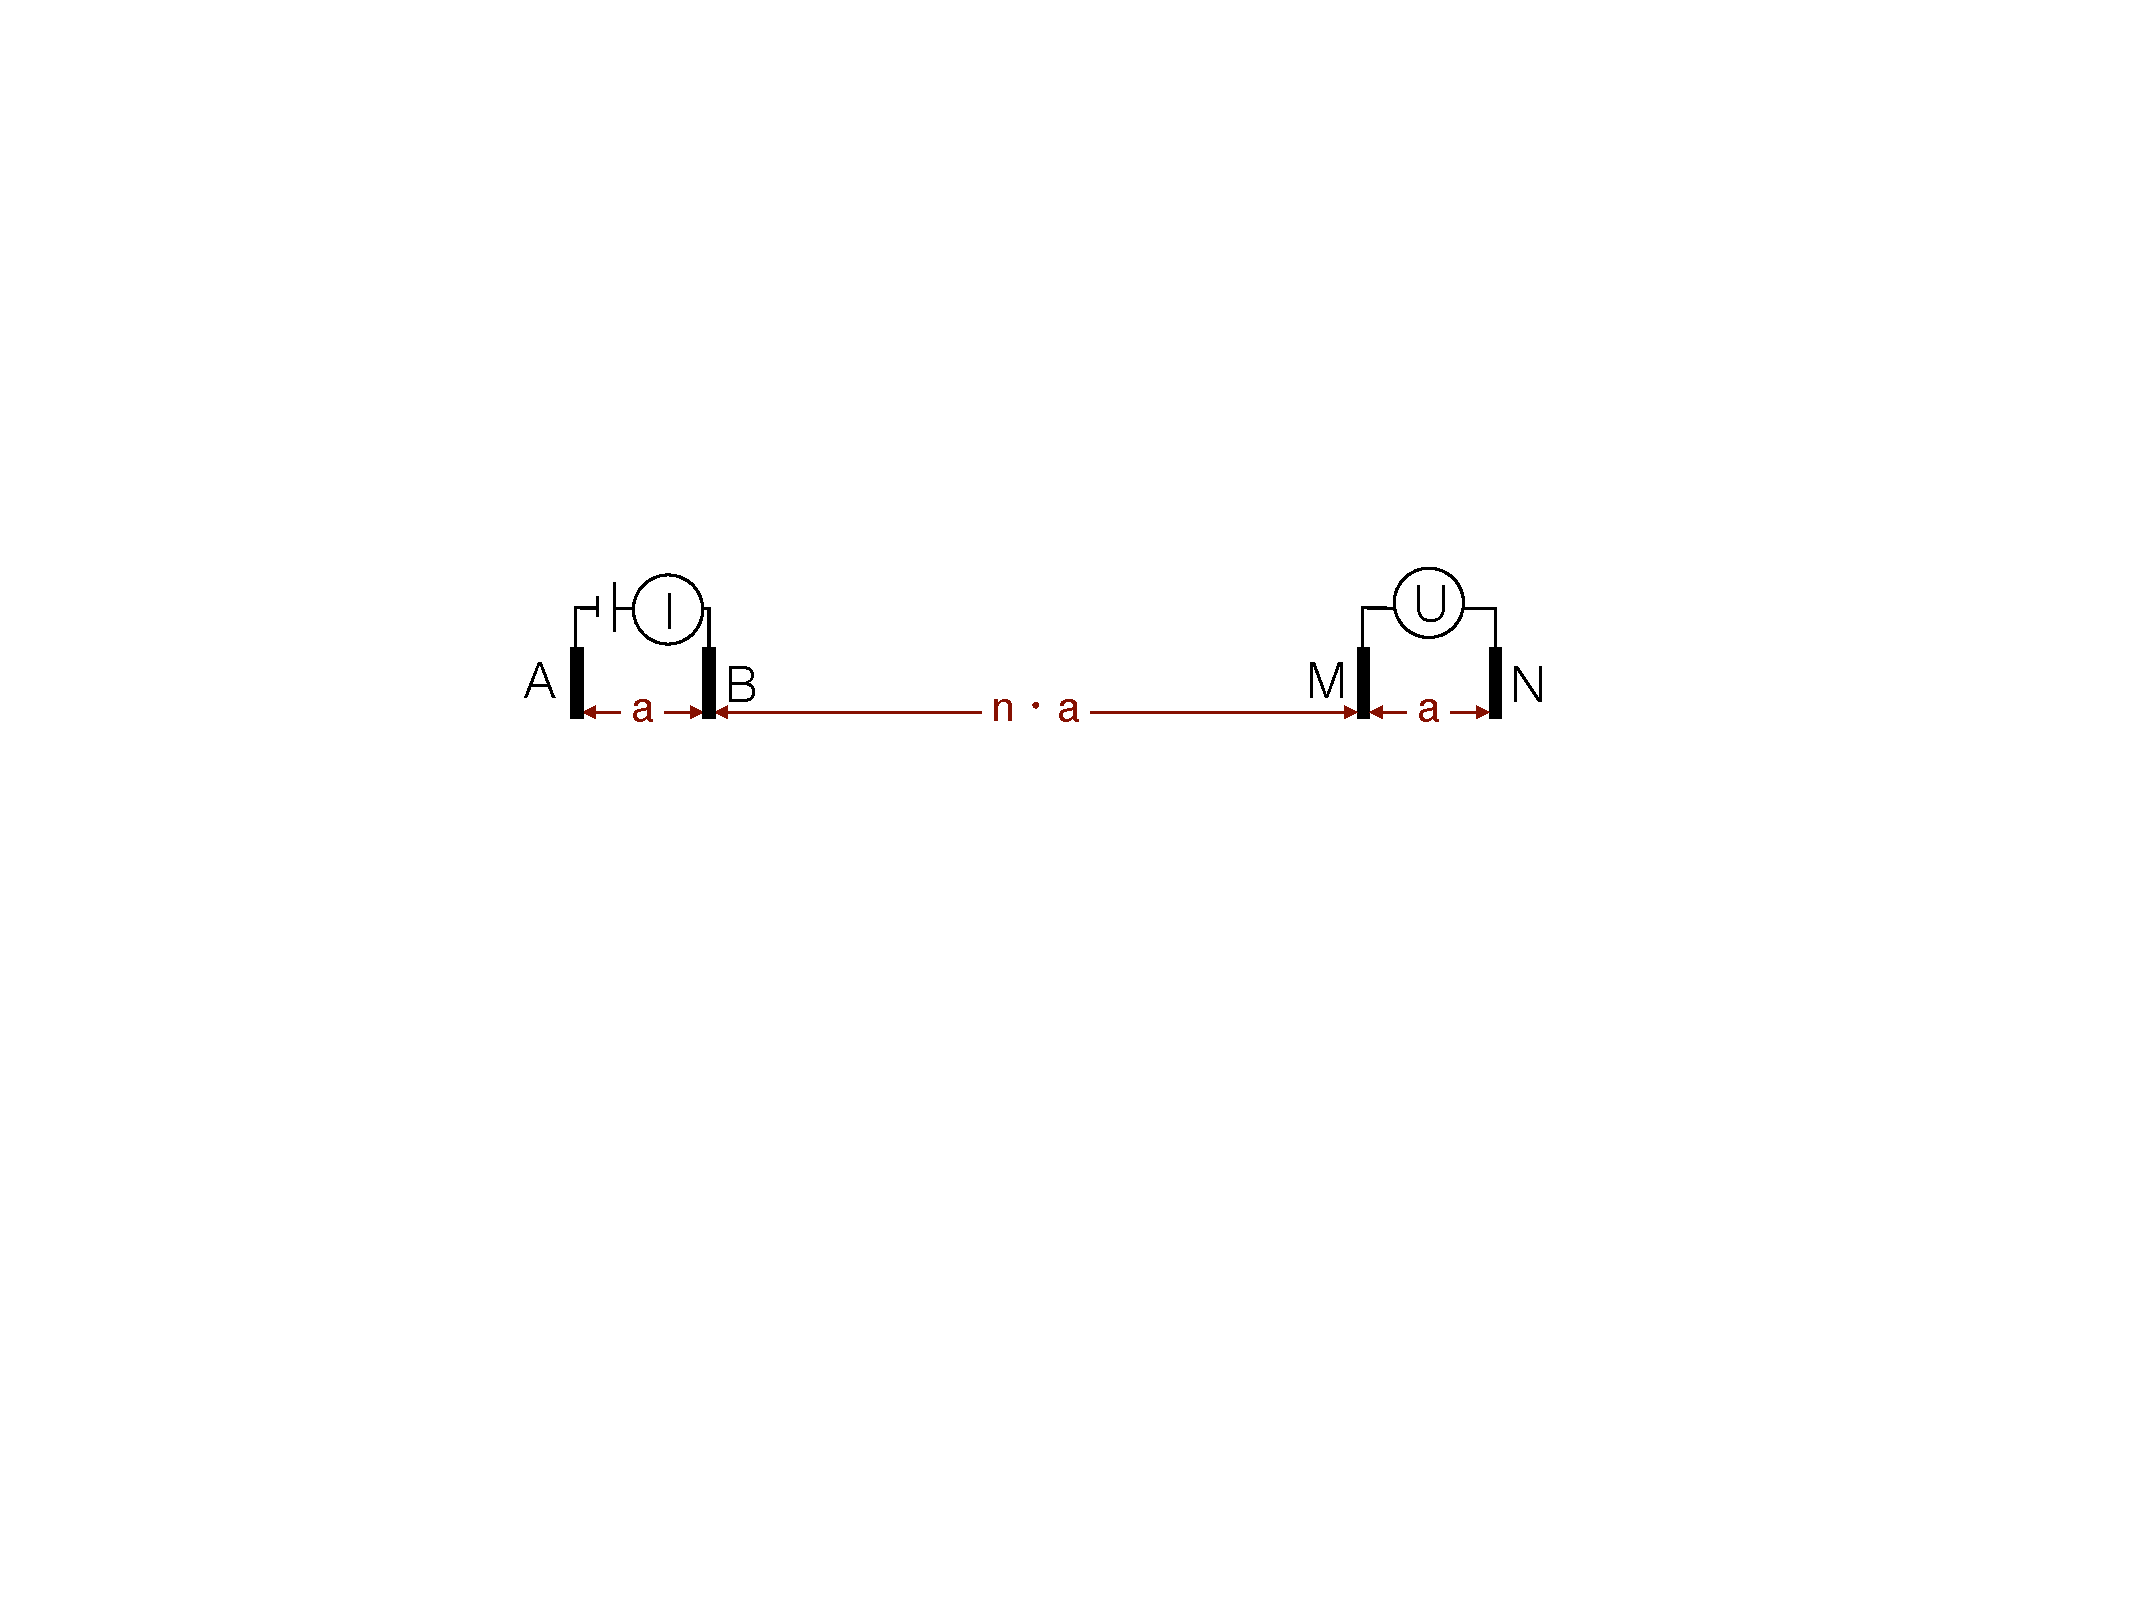
\includegraphics[scale = 0.35]{GeoelektrikBilder/DipolDipolAnordnung}
	\end{subfigure}
	\begin{subfigure}[m]{0.5\textwidth}
		\begin{equation*}
				K = \pi \cdot a \cdot n \cdot (n+1) \cdot (n+2)
		\end{equation*}
	\end{subfigure}
\end{figure}


\subsection{Stromfluss im Halbraum}
Bei einer Messung mit Vierpunktanordnung wird Strom in die Erde eingespeist. Dadurch entsteht ein elektrisches Feld, welches sich durch Feldlinien charakterisieren lässt. Diese Feldlinien sind senkrecht zur Stromrichtung und bilden Äquipotentialflächen, also Flächen, an denen das gleiche Potential anliegt.   

\begin{figure}[H]
	\centering
	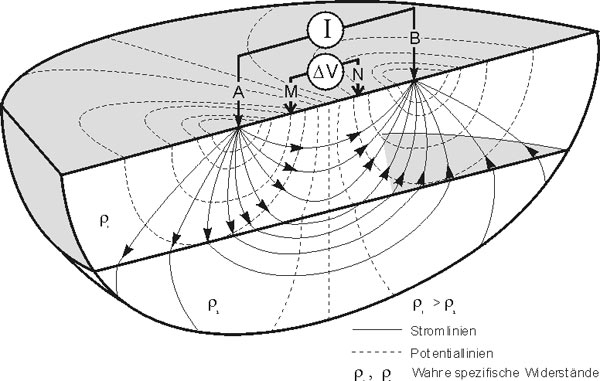
\includegraphics[width = \textwidth]{GeoelektrikBilder/EFeldErde}	
	\caption*{\textsl{Quelle: umwelt.sachsen.de}}
\end{figure}

 





	\chapter{Gravimetrie}


Das Ziel einer gravimetrischen Messung ist die Untersuchung des Untergrunds auf Anomalien der Dichte, um die Massenverteilung rekonstruieren zu können. Damit lassen sich beispielsweise Unterschiede im Gestein lokalisieren. \par

 Hierzu vermisst man das lokale Schwerefeld der Erde, das durch Dichteunterschiede im Boden geringfügig verändert wird. Um diese Änderungen messen zu können, werden hoch empfindliche Messgeräte verwendet.\par
 
 Im Folgenden werden wir uns mit zugrunde liegenden physikalischen Prinzipien, sowie den Störfaktoren und deren Korrektur beschäftigen. Weiterhin wird es einen kurzen Einblick in die Messmethodik geben.

\section{Physikalische Grundlagen}


\subsection*{Gravitationsgesetz}
Die Anziehung zweier punktförmiger Massen wird durch das Newton'sche Gravitationsgesetz beschrieben. Hierbei bezeichnet $|\vec{F}|$ den Betrag der vektoriellen Kraft, $m_1$ und $m_2$ die betrachteten Massen, $r$ den Abstand der Massenmittelpunkte und $G$ die Gravitationskonstante. Letztere ist eine universelle Größe und gilt in allen Bezugssystemen. 

\begin{equation*}
	|\vec{F}| = G \frac{m_1 \cdot m_2}{r^2} \quad \text{mit}\quad G = 6,67 \cdot 10^{-11}\,\frac{\si{m^3}}{\si{kg s^2}}
\end{equation*} 

\begin{figure}[H]
  \centering
  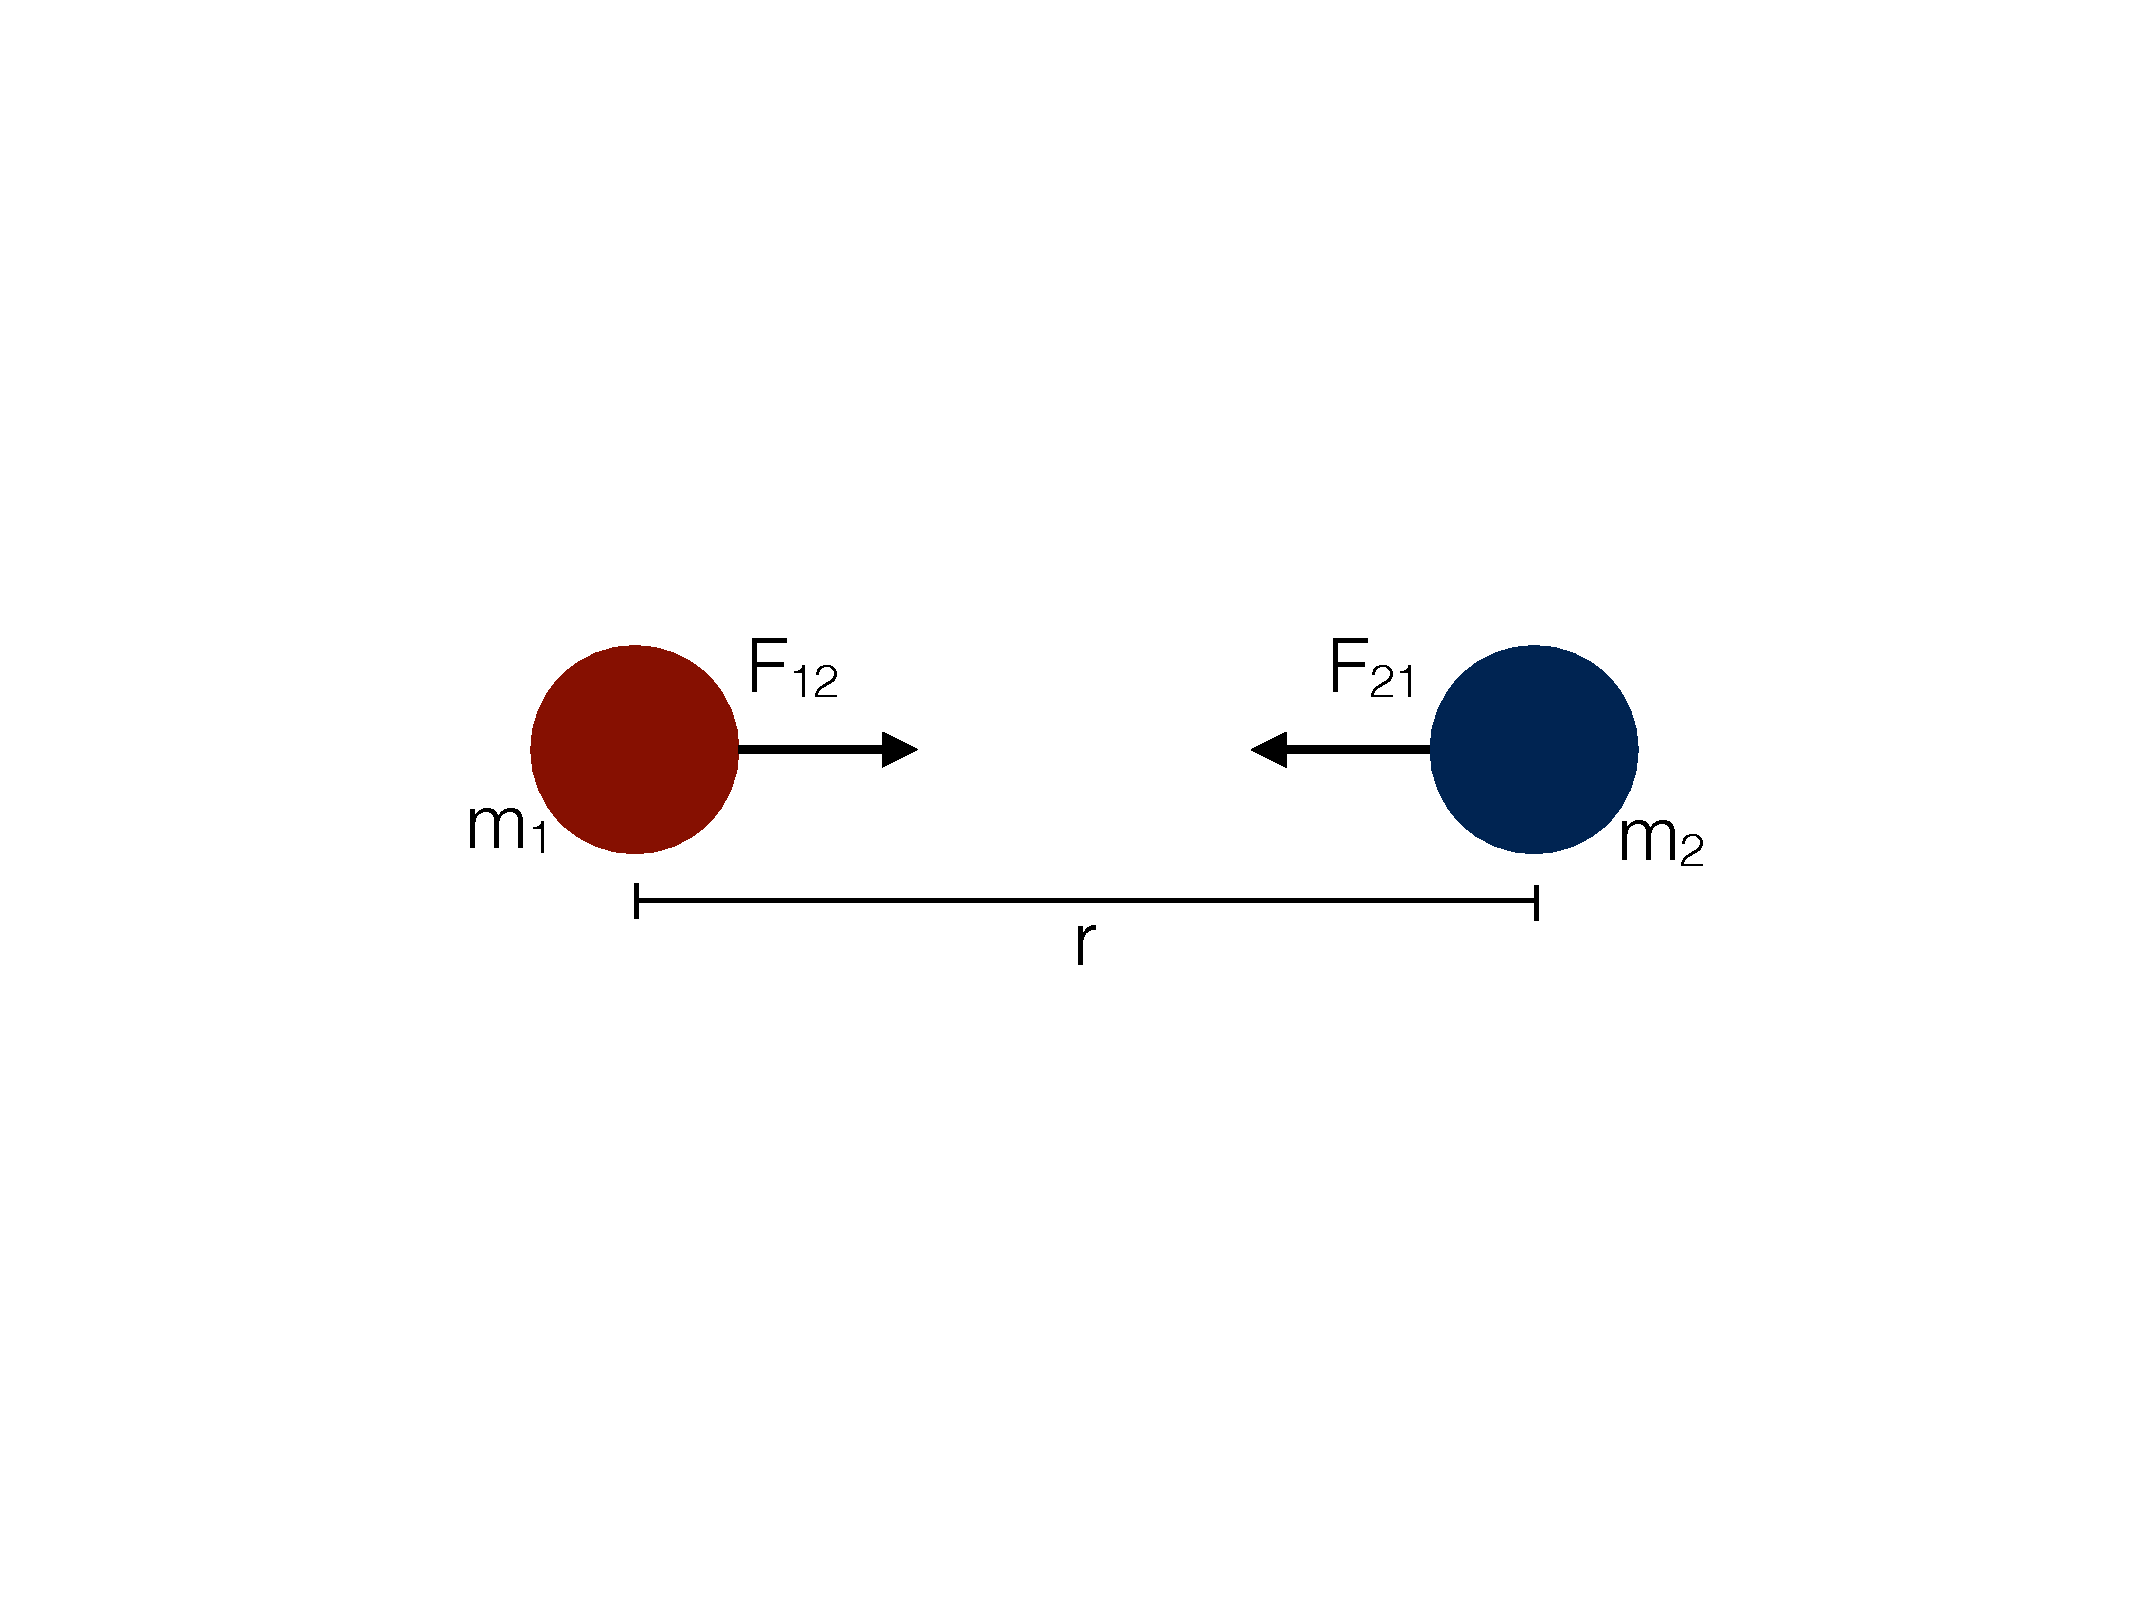
\includegraphics[width = \textwidth]{GravimetrieBilder/GravitationGrafik}
\end{figure}

\section{Das Schwerefeld und die Figur der Erde}

Betrachten wir nun das Gravitationsgesetz im Bezug zur Erde. Dabei gehen wir von einer Kugelerde mit Radius $R = 6371\,\si{km} $ aus.\\
Wir bezeichnen die Masse der Erde für den Rest dieses Kapitels mit $M$ und eine beliebige Masse an der Erdoberfläche mit $m$. In der folgenden Formel berechnen wir die Erdanziehungskraft eines Objekts mit Masse $m$: 


\begin{figure}[H]
	\begin{subfigure}[m]{0.5\textwidth}
	\centering
		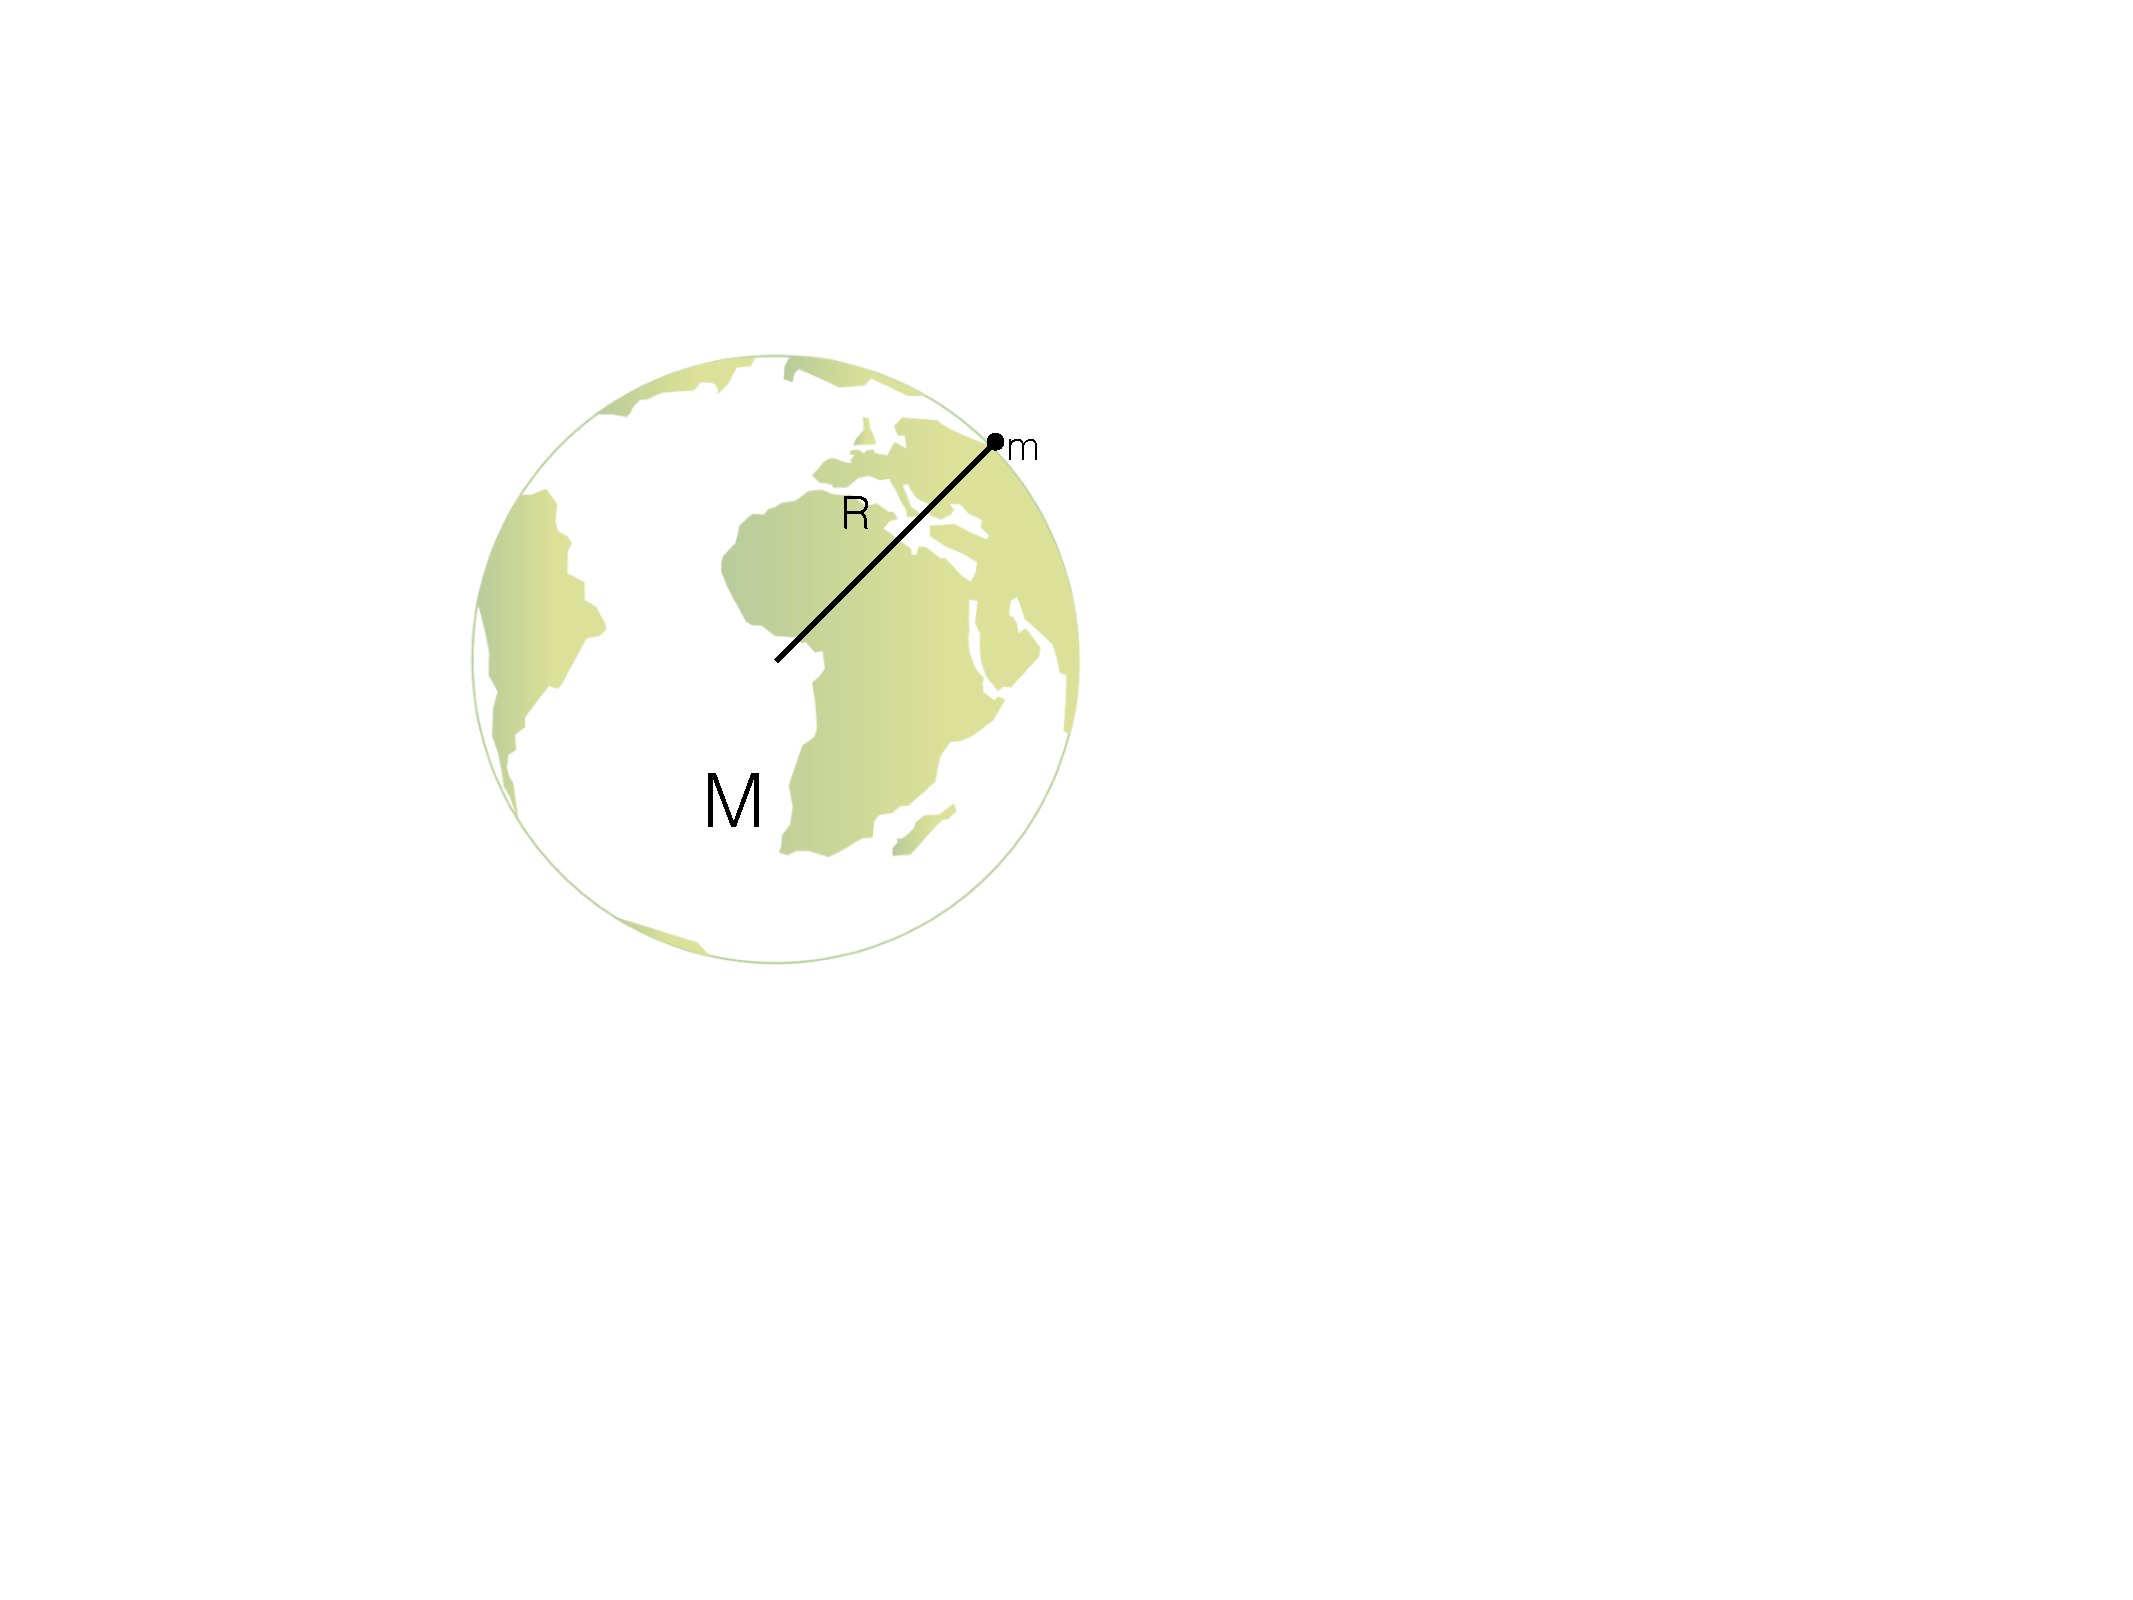
\includegraphics[scale=0.3]{GravimetrieBilder/Erde_mit_Masse_und_Radius}
	\end{subfigure}
	\begin{subfigure}[m]{0.5\textwidth}
	\centering
		\[\begin{aligned}
			|\vec{F}| = \frac{G\cdot M}{R^2} \cdot m = g_0 \cdot m
		\end{aligned}\]
	\end{subfigure}
\end{figure}


$g_0$ ist die Normalbeschleunigung, also die mittlere Fallbeschleunigung auf der Erdoberfläche:

\begin{equation*}
	g_0 = 9,81\,\frac{\si{m}}{\si{s^2}} = 981\,\frac{\si{cm}}{\si{s^2}} = 981\,\si{Gal}
\end{equation*} 

Die nachfolgende Grafik stellt die Schwerebeschleunigung in Abhängigkeit vom Abstand vom Erdmittelpunkt dar. Wir beobachten, dass im Erdmittelpunkt \mbox{$g=0$} gilt und die Schwerebeschleunigung danach bis zu ihrem Maximum $g_0$ bei $R$ linear zunimmt. Für Abstände größer als den Erdradius nimmt sie proportional zu $1/r^2$ ab und geht gegen Null. 

\begin{figure}[H]
\centering
  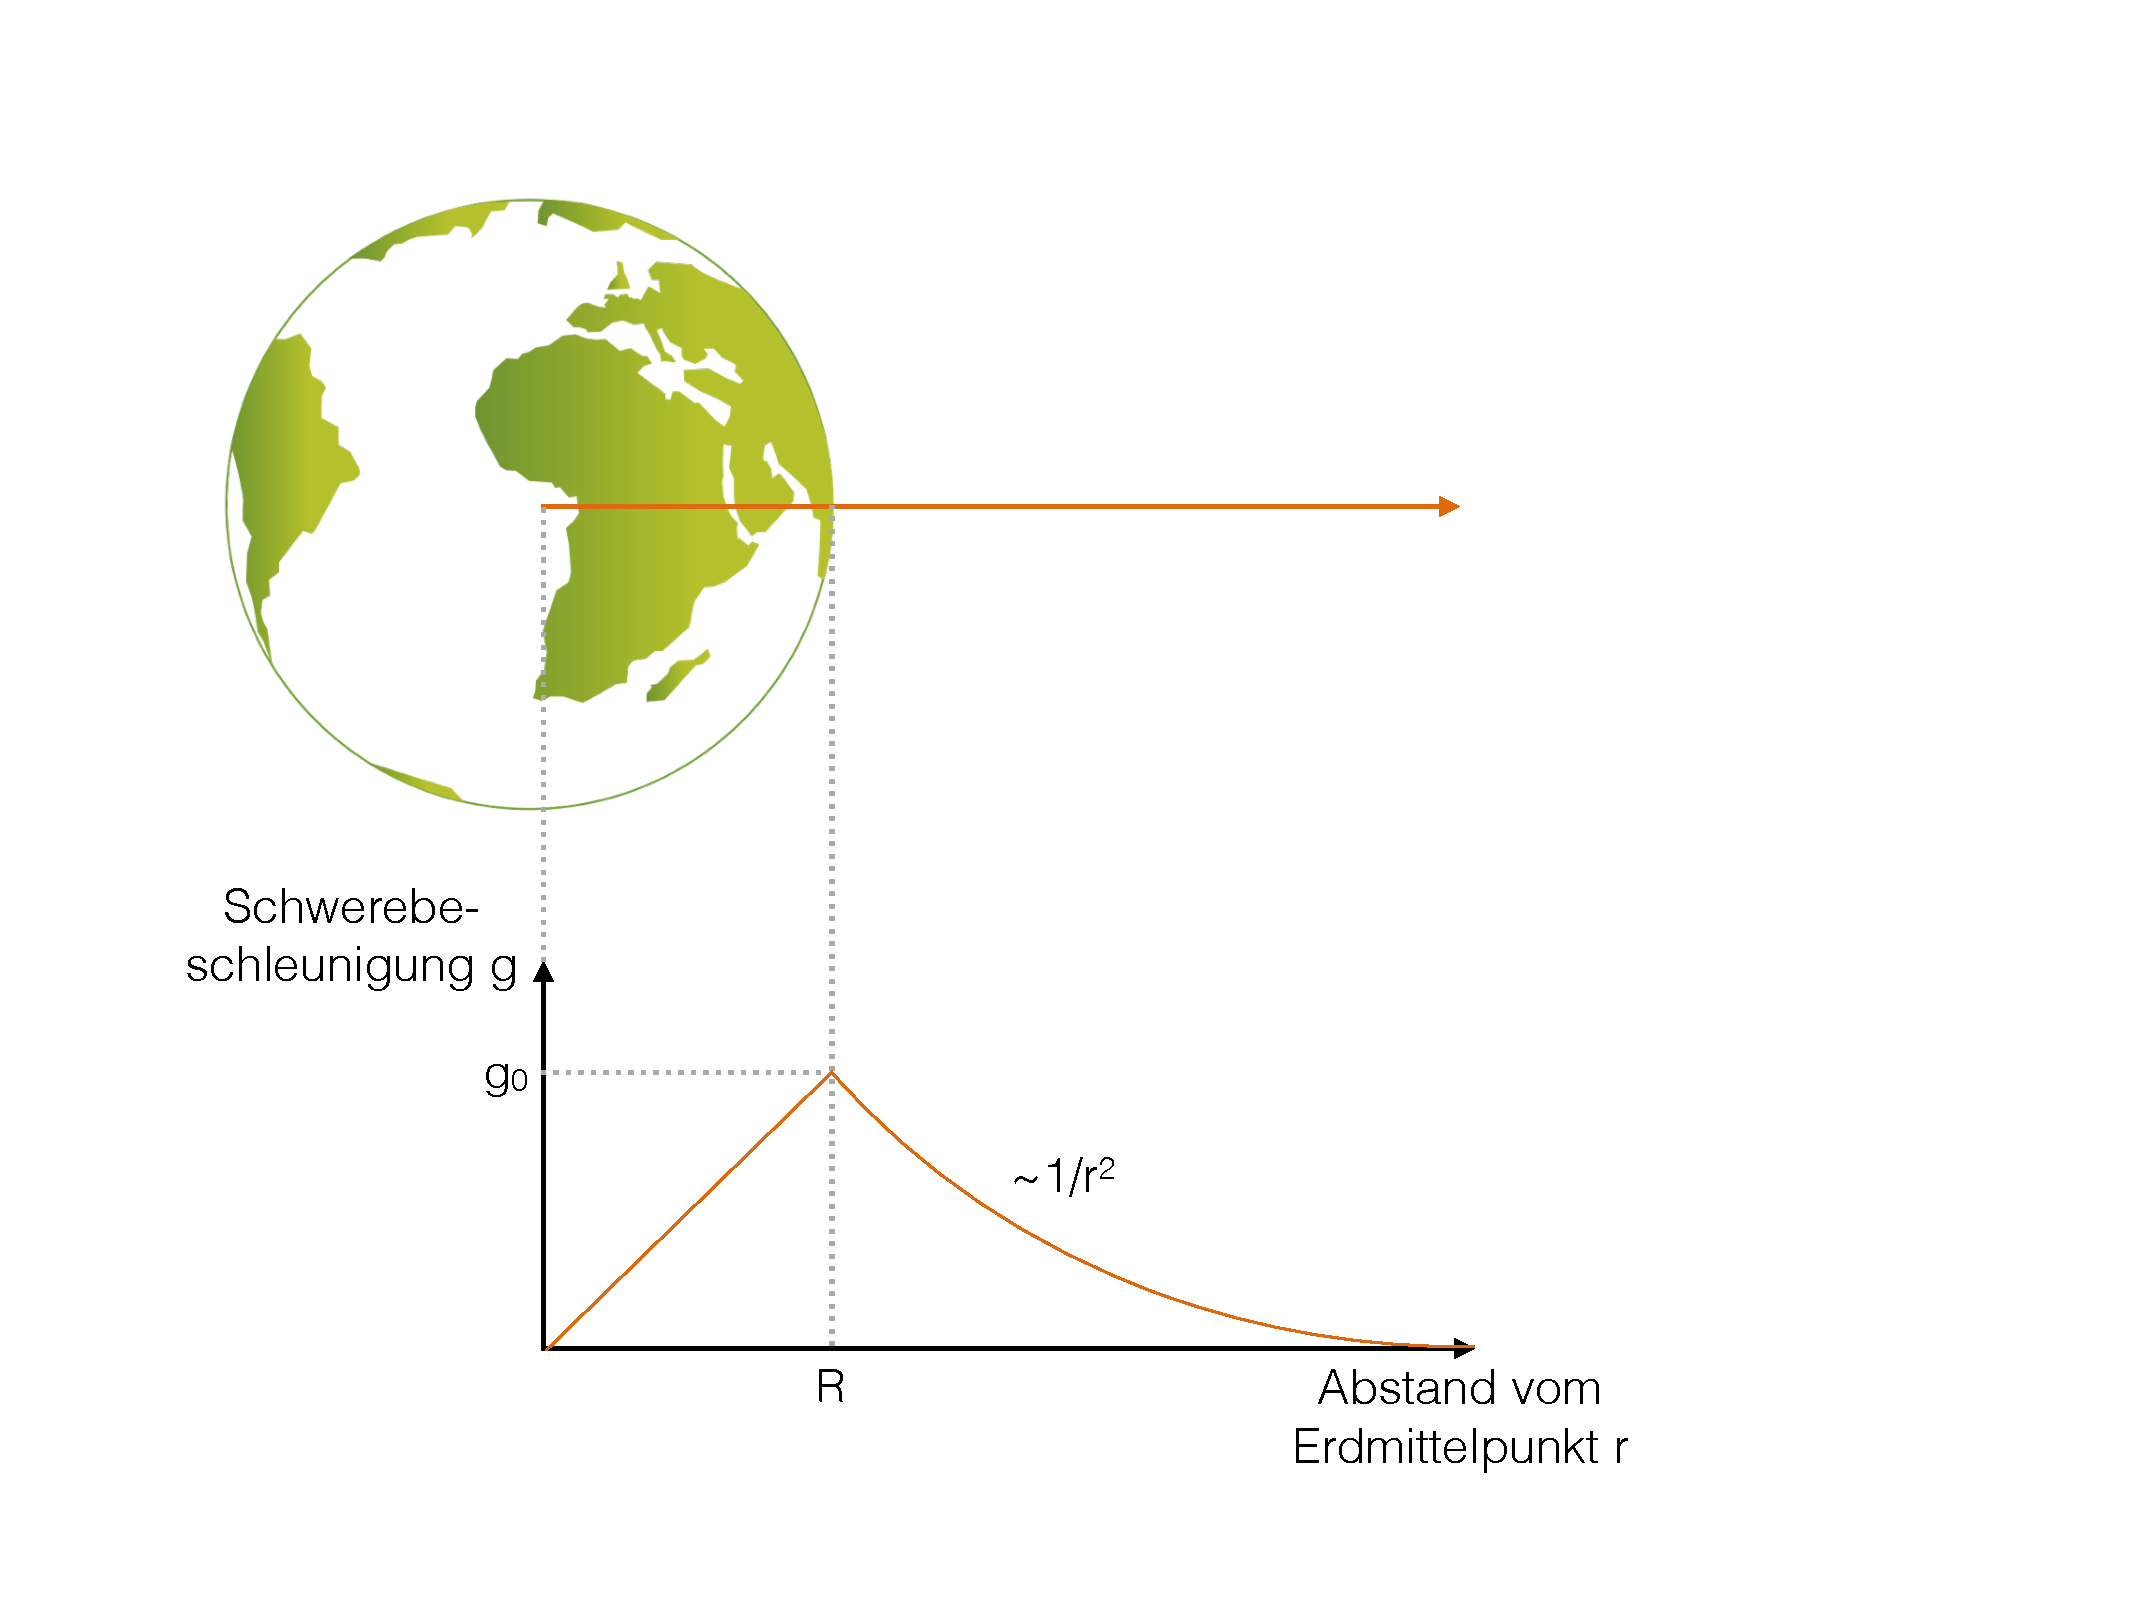
\includegraphics[width = \textwidth]{GravimetrieBilder/Abnahme_Grav}
\end{figure}


\subsection*{Die Erde als Kugel}

Wie bereits genannt, haben wir für diese Berechnungen angenommen, dass die Erde eine perfekte Kugel ist. Dies ist aber nicht der Fall. Eine bessere Näherung wäre ein Ellipsoid, wie wir später noch sehen werden. Die Abweichungen vom Kugelmodell entstehen durch verschiedene Faktoren: 
\begin{itemize}
	\item Inhomogenität der Erde
	\item gravitativer Einfluss durch Planeten, Gestirne (z.B. Sonne, Mond)
	\item gravitativer Einfluss durch Luftmassen in der Atmosphäre
	\item Fliehkraft durch Erdrotation
\end{itemize} 


Betrachten wir einmal den Einfluss dieser Faktoren auf eine gravimetrische Messung.  \begin{itemize}
	\item gravitativer Einfluss Mond: $\approx 82\,\si{\mu Gal}$
	\item gravitativer Einfluss Sonne: $\approx 38\,\si{\mu Gal}$
	\item Luftmassen: bis zu $900\,\si{\mu Gal}$
\end{itemize}
Vergleicht man diese Werte mit der Normalbeschleunigung ($981\,\si{Gal}$) und der Genauigkeit eines Messgerätes ($\approx 1\,\si{\mu Gal}$), ist offensichtlich, dass diese Variationen bei der Auswertung nicht vernachlässigt werden dürfen.

Dabei sei noch darauf hingewiesen, dass die Effekte von Sonne und Mond tagesabhängig sind, während sich der Einfluss durch Luftmassen ständig verändert. 


Mit dem formgebenden Faktor Fliehkraft beschäftigen wir uns nun noch genauer.
 
\subsubsection*{Fliehkraft durch Erdrotation}

Da sich durch die Fliehkraft die Form der Erde von der Kugel abhebt, ändert sich auch die Berechnung der lokalen Schwerebeschleunigung: \begin{equation*}
	g(\varphi) = \frac{G \cdot M}{R^2} - \omega^2 \cdot R \cdot cos^2(\varphi)
\end{equation*} 
Den ersten Teil der Formel vor dem Minus kennen wir bereits als Normalschwere, der hintere Teil ist neu. Dieser Teil ist die Zentrifugalbeschleunigung in tangetiale Richtung, in Abhängigkeit von der geozentrischen Breite. Die Erklärung was das bedeutet und wie dieser Teil sich herleiten lässt schauen wir uns nun an. Dazu betrachten wir diese Grafik:  

\begin{figure}[H]
\centering
  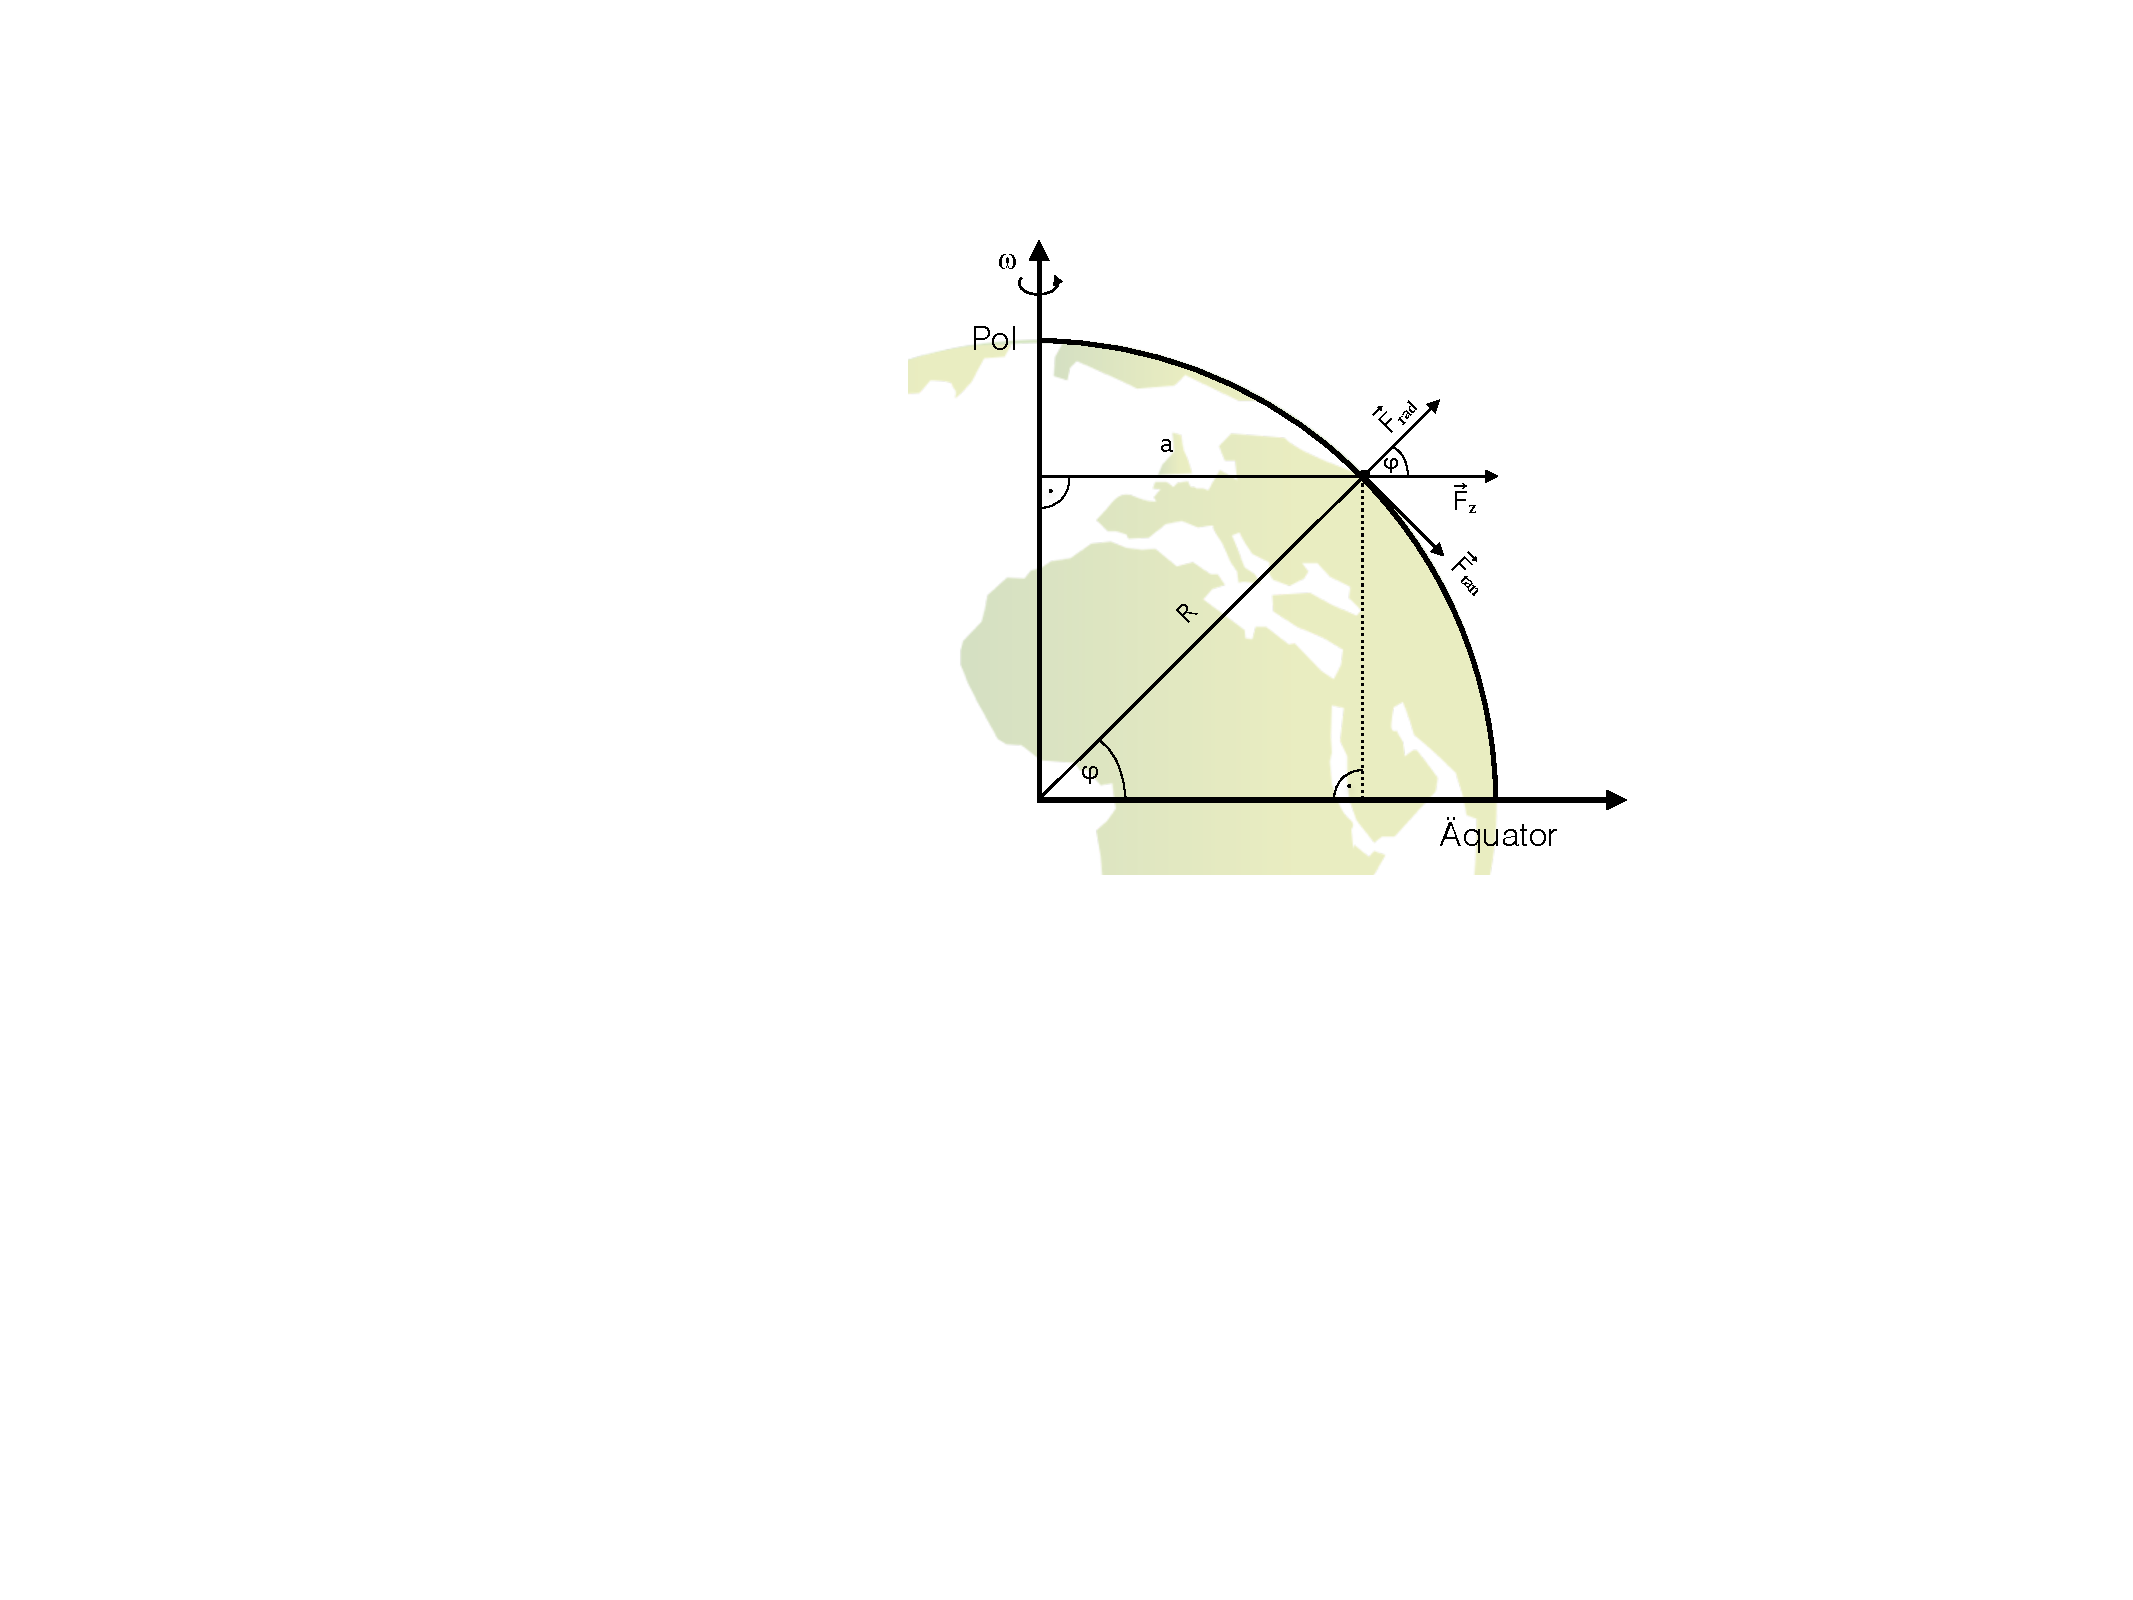
\includegraphics[width = \textwidth]{GravimetrieBilder/Fliehkraft}
\end{figure}

$\omega$ steht für die Drehgeschwindigkeit, also wie schnell sich die Erde um ihre eigene Achse dreht. Eine Umdrehung dauert, wie wir wissen, einen Tag. $\omega$ berechnet sich dann so: \begin{equation*}
	\omega = \frac{2 \pi}{1 \,\si{Tag}} = \frac{2 \pi}{24 \cdot 60 \cdot 60\,\si{s}} = \frac{2 \pi}{86400\,\si{s}} \approx 7,29 \cdot 10^{-5}\,\si{\frac{rad}{s}}
\end{equation*}

Den direkten Abstand einer Masse an der Erdoberfläche bezeichnen wir mit $a$ und den Erdradius mit $R$. 
$\varphi$ gibt die geozentrische Breite an, also auf welchem Breitengrad wir uns befinden. Am Äquator ist $\varphi$ = 0, am Nordpol gilt $\varphi$ = 90. Karlsruhe liegt ungefähr bei 49° nördliche Breite.

Übrig bleiben nun noch die drei Kräfte, die wir uns jetzt noch anschauen wollen. 
Die Zentrifugalkraft $|\vec{F}_z|$  wirkt senkrecht zur Rotationsachse und beschleunigt ein Objekt von ihr weg. Wir kennen das beispielsweise aus einem Karussell. Berechnen lässt sich die Zentrifugalkraft folgendermaßen: \begin{equation*}
	|\vec{F}_z| = m \cdot a \cdot \omega^2 = m \cdot b \quad \text{mit} \quad b = a \cdot \omega^2  
\end{equation*} $b$ ist hierbei die Zentrifugalbeschleunigung. 

Nehmen wir nun einmal an, dass wir den Abstand $a$  zur Rotationsachse nicht kennen. Um die Zentrifugalkraft berechnen zu können ist er aber essenziell. Betrachten wir noch einmal das Schaubild, besonders die gepunktete Linie von der x-Achse zu unserer Masse auf der Erdoberfläche: \begin{equation*}
	a = R \cdot cos(\varphi) 
	\end{equation*} 
Damit lässt sich die Zentrifugalkraft auch schreiben als \begin{equation*}
	|\vec{F}_z| = m \cdot a \cdot \omega^2 = m \cdot R \cdot cos(\varphi) \cdot \omega^2
\end{equation*}
Uns interessiert aber eigentlich nicht die totale Zentrifugalkraft, sondern nur der radiale Anteil $\vec{F}_{\text{rad}}$ , da dieser die Abweichung des Radius von der Kugel angibt. Um diesen Anteil berechnen zu können, teilen wir $\vec{F}_z$ auf in den gesuchten radialen, und einen tangentialen Anteil, die senkrecht zueinander sind. Um dies umzusetzen machen wir wieder einfache geometrische Überlegungen. \begin{equation*}
	|\vec{F}_{\text{rad}}| = |\vec{F}_z| \cdot cos(\varphi) = m \cdot b \cdot cos(\varphi) = m \cdot \omega^2 \cdot R \cdot cos^2(\varphi) 
\end{equation*} Dabei ist $\omega^2 \cdot R \cdot cos^2(\varphi)$ die Zentrifugalbeschleunigung in radialer Richtung. 
Zur Vollständigkeit sei auch noch der tangentiale Anteil genannt:  \begin{equation*}
	|\vec{F}_{\text{tan}}| = \frac{\omega^2 \cdot R}{2} sin(2\varphi) \cdot m 
\end{equation*}

Wir kennen nun die Beschleunigung der Erde durch Rotation in tangentiale Richtung und können damit die Schwerebeschleunigung auf einer rotierenden Kugel berechnen:  \begin{equation*}
	g(\varphi) = \frac{G \cdot M}{R^2} - \omega^2 \cdot R \cdot cos^2(\varphi) 
\end{equation*}

\subsection*{Näherungen an die Figur der Erde}
\subsubsection{(1) Kugel}
Die Näherung als Kugel haben wir bereits kennen gelernt. 

\subsubsection{(2) Referenzellipsoid}
Wählt man die Ellipse als Erdmodell, beachtet man die Verformung durch Fliehkräfte. Dadurch wird der Abstand von Pol zu Pol kleiner als die Hauptachse der Ellipse. Die jeweiligen Abweichungen von der Kugelerde sind jedoch relativ gering. 

\begin{figure}[H]
	\begin{subfigure}[m]{0.5\textwidth}
	\centering
		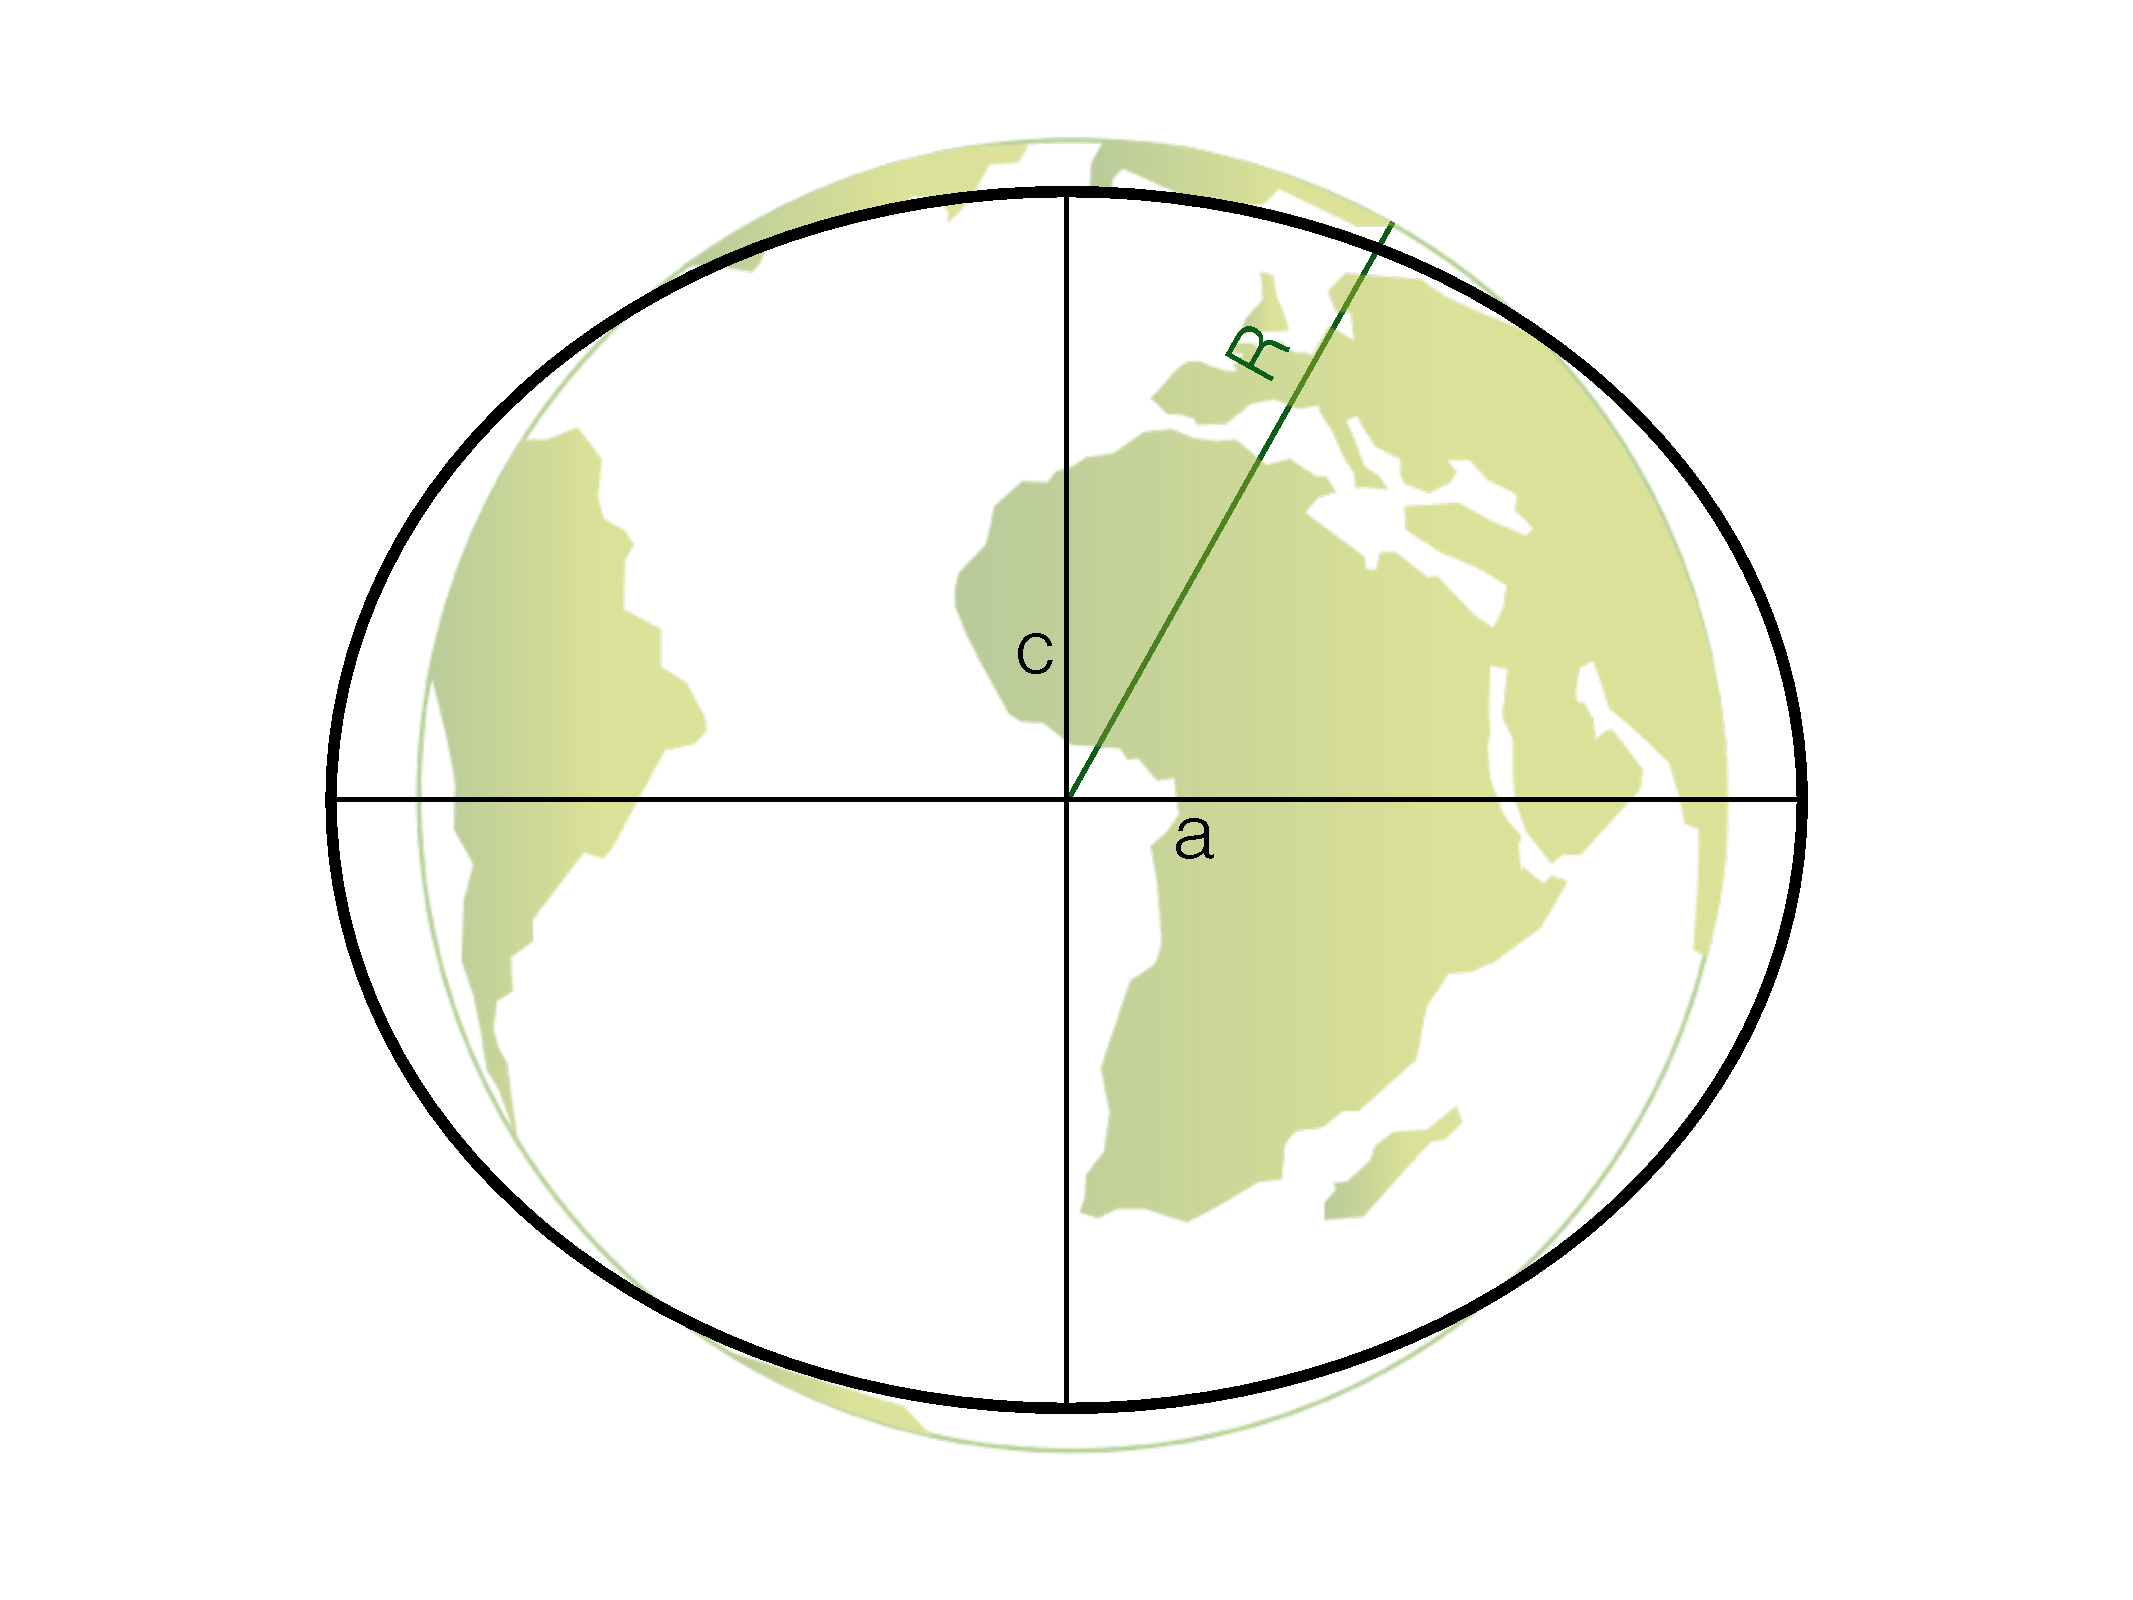
\includegraphics[scale=0.2]{GravimetrieBilder/Referenzellipsoid}
	\end{subfigure}
	\begin{subfigure}[m]{0.5\textwidth}
	\centering
		\[\begin{aligned}
			a &= 6378,136\,\si{km}\\
	c &= 6356, 751\,\si{km}\\
	R - a &\approx 7\,\si{km}\\
	R - c &\approx 15\,\si{km}
		\end{aligned}\]
	\end{subfigure}
\end{figure}

\subsubsection{(3) Geoid}
Die Gravitationskraft auf der Erde, also die Schwerkraft ist eine konservative Kraft. Das bedeutet zum einen, dass es ein Potential zur Kraft gibt. Dieses Schwerepotential $W$ wird über den Gradienten und das Vektorfeld der Schwerebeschleunigung definiert.
\begin{equation*}
	\vec{g} = - \text{grad}(W) = \left( \frac{\partial W}{\partial x}, \frac{\partial W}{\partial y}, \frac{\partial W}{\partial z} \right)^{\text{T}}	
\end{equation*} 
Weiterhin bedeutet es aber auch, dass es Äquipotentialflächen der Schwerebeschleunigung gibt. Anschaulich:

\begin{figure}[H]
	\centering
	\includegraphics[width = \textwidth]{GravimetrieBilder/Äquipotentialflächen}
\end{figure}
Entlang solcher Flächen erfordert das Bewegen einer Masse keine Arbeit. 

Die Oberflächen ruhender Ozeane oder Seen sind solche Äqupotentialflächen. Als Geoid bezeichnet man nun die Äquipotentialfläche, die dem mittleren Niveau aller Ozeane entspricht. Es gilt also \begin{equation*}
	W = W_{\text{Geoid}} = \text{konst.}
\end{equation*}

\begin{figure}[H]
	\centering
	\includegraphics[width = \textwidth]{GravimetrieBilder/Geoid}
\end{figure}

Abweichungen des Geoid vom Referenzellipsoiden werden als Geoidundulationen bezeichnet. Diese Abweichungen bewegen sich zwischen etwa -105\,m im nördlichen indischen Ozean und ungefähr +70\,m nördlich von Papua-Neuguinea. 

\begin{figure}[H]
  \includegraphics[width = \textwidth]{GravimetrieBilder/Geoidundulation}
  \caption*{Globale Geoidundulation. \textit{Quelle: Wikipedia}}
\end{figure}

Es sei noch darauf hingewiesen, dass für gravimetrische Messungen die Erde als Kugel bzw. als Ellipsoid angenähert wird. Zwar wäre ein Geoid die richtige Näherung, aber sie lässt sich nur schwer mathematisch beschreiben und eignet sich für das Berechnen der Schwerekorrekturen daher nicht. 


\section{Schwerereduktionen}

\begin{figure}[H]
	\centering
	\includegraphics[width = \textwidth]{GravimetrieBilder/Schwerereduktionen}
\end{figure}

Das Ziel einer gravimetrischen Messung ist die Darstellung einer lokalen Schwereanomalie im Untergrund, die durch Dichteanomalien (Grafik: $\Delta \rho$) hervorgerufen wird. Da die Messgeräte hoch empfindlich sind müssen diverse Störfaktoren der Umwelt und Umgebung korrigiert werden. Diese Korrekturen werden unabhängig voneinander berechnet.  
\begin{enumerate}
	\item Wirkung der gesamten Erde \begin{itemize}
		\item Normalschwerereduktion $\gamma_0$
		\item Wirkung der Zentrifugalbeschleunigung (abhängig von geographischer Breite): Breitenreduktion $\delta_{\gamma_0}$
		\end{itemize}
	\item Höhenunterschiede: Freiluftreduktion $\delta_{g_{FL}}$
	\item Wirkung der Gesteinsmasse: Bouger-Reduktion $\delta_{g_B}$
	\item Topographie der Umgebung: Topographische Reduktion $\delta_{g_{\text{Top}}}$
	\item Zeitabhängige Faktoren: Gerätegang, Gezeiten,\dots \space$g(t)$
\end{enumerate} 
Die Schwereanomalie errechnet sich dann mit folgender Formel: 
\begin{equation*}
	\Delta g = g(x,y,z,t) - g(t) - \delta_g (x,y,z)
\end{equation*}
Dabei ist $g(x,y,z,t)$ die gemessene Schwerebeschleunigung, $g(t)$ sind die zeitabhängigen Faktoren und $\delta_g (x,y,z)$ die ortsabhängigen Faktoren. 
Im Folgenden werden wir die ortsabhängigen Faktoren und ihre Berechnung genauer betrachten. 

\subsection{Wirkung der gesamten Erde}
\subsubsection{Normalschwerereduktion}

\begin{description} 
	\item rotierende Kugel: Diese Formel kenn wir bereits aus Kapitel 7.2. Auch ihre Herleitung haben wir dort bereits betrachtet. \begin{equation*}
		\gamma_0 = g(\varphi) = \ub{\frac{G \cdot M}{R^2}}{\gamma_0} - \ub{\omega^2 \cdot R \cdot cos^2(\varphi_B)}{\substack{\text{Zentrifugal-} \\ \text{beschleunigung}}}
	\end{equation*}
	
	\item rotierendes Ellipsoid: \begin{equation*}
		\gamma_0 = g_{\text{Ellips.}} = 9,7803 \cdot (1 + 0,0053 \cdot sin^2(\varphi_B) - 5,8 \cdot 10^{-6} sin^2(\varphi_B))
	\end{equation*} Wir wollen nicht näher darauf eingehen wie diese Formel zustande kommt.
\end{description}

\subsubsection{Breitenreduktion} 
Aus der obigen Gleichung der Normalschwere für den Rotationsellipsoiden lässt sich die Breitenkorrektur berechnen. Diese ist abhängig von der geographischen Breite $\varphi_B$ des Referenzpunktes $R$, da die Schwerebeschleunigung auf dem Referenzellipsoiden in Richtung der Pole zunimmt. \begin{equation*}
	\delta_{\gamma_0} = 0,00081 \cdot sin^2(2 \cdot \varphi_B) \cdot \Delta y
\end{equation*}
$\Delta y$ bezeichnet hierbei die Abweichung des Messpunktes vom Referenzpunkt in Nord-Süd-Richtung in\,km. 

\begin{figure}[H]
	\centering
	\includegraphics[scale = 0.3]{GravimetrieBilder/Breitenreduktion}
\end{figure}

\subsection{Freiluftreduktion}

\begin{figure}[H]
	\centering
	\includegraphics[width = \textwidth]{GravimetrieBilder/Freiluftreduktion}
\end{figure}

Bei einer gravimetrischen Messung wird ein Bezugsniveau festgelegt, auf das alle Messpunkte normiert werden. Dieses Bezugsniveau kann beispielsweise das Normalnull sein. Grund für eine Normierung ist der Abstand der Messpunkte vom Erdmittelpunkt, also unterschiedliche Radien. Die Schwerebeschleunigung nimmt aber mit höherem Radius ab. Diesen Unterschied gleicht man mit der Freiluftkorrektur aus. \begin{align*}
	\delta_{g_{FL}} &= G \cdot \left( \frac{M}{(R + h)^2} - \frac{M}{R^2} \right) \\
	&\approx -2 \cdot \frac{G \cdot M}{R^2} \cdot \frac{h}{R} = -2 \cdot \gamma_0 \frac{h}{R} \approx -0,3086 \cdot h\,\si{m Gal}
\end{align*}
Die Höhenmessung wird mit DGPS durchgeführt und hat eine Genauigkeit von ungefähr 3\,cm: \begin{equation*}
	\Delta (\delta_{g_{FL}}) \leq 0,01\,\si{m Gal} \quad \Rightarrow \quad \Delta h = \frac{1}{0,3086} \cdot \Delta (\delta_{g_{FL}}) \approx 0,03\,\si{m}
\end{equation*}
\subsubsection{Freiluftanomalie} 
Die Freiluftanomalie ist eine erste Berechnung der Dichteanomalie im Untergrund. Bei dieser Anomalie sind zusätzlich zu den zeitabhängigen Faktoren nur Normalschwerereduktion und Höhenkorrektur mit eingerechnet. \begin{equation*}
	\Delta g_{FL} = g(x, y, z, t) - g(t) - \gamma_0 - \delta_{\gamma_0} - \delta_{g_{FL}}
\end{equation*}

\subsection{Bouguer-Reduktion}
Bringt man die Messpunkte auf ein Bezugsniveau, muss nicht nur die Schwereveränderung durch die Höhe, sondern auch die Schwerewirkung der zwischenliegenden Gesteinsmasse eingerechnet werden. 

\begin{figure}[H]
	\centering
	\includegraphics[width = \textwidth]{GravimetrieBilder/Bouguer-Reduktion1}
\end{figure}

Diese Gesteinsmasse wird als Platte angenähert, die in alle Seiten ins unendliche ausgedehnt ist und Mächtigkeit (Reduktionshöhe) $h$ und homogene Massendichte $\rho$ hat. 

\begin{figure}[H]
	\centering
	\includegraphics[width = \textwidth]{GravimetrieBilder/Bouguer-Reduktion2}
\end{figure}

Ihre Schwerewirkung berechnet sich so: \begin{equation*}
	\delta_{g_B} = 2 \pi \cdot G \cdot \rho \cdot h
\end{equation*}
Wir betrachten ein Beispiel: \begin{align*}
	&h = 10\,\si{m}, \quad \rho = 2,39\,\si{\frac{kg}{m^3}} \quad \text{(Sedimentgestein)}\\
	&\Rightarrow \delta_{g_B} = 1\,\si{m Gal}
\end{align*}

\subsubsection{Bouguer-Anomalie}
Im Gegensatz zur Freiluftanomalie rechnet man bei der Bouguer-Anomalie die Bouguer-Korrektur, also die Korrektur der Schwerewirkung der Gesteinsmasse, mit ein. Diese Berechnung spiegelt die Dichteanomalie im Untergrund gut wider. \begin{equation*}
	\Delta g_{FL} = g(x, y, z, t) - g(t) - \gamma_0 - \delta_{\gamma_0} - \delta_{g_{FL}} - \delta_{g_B}
\end{equation*} 

\subsection{Topographische Reduktion}
Bei der Bouguer-Reduktion haben wir bereits gelernt, dass Gesteinsmassen einen Einfluss auf das Messergebnis haben. Das heißt, dass wir nicht nur die Gesteinsmasse zwischen Bezugsniveau und Messpunkt, sondern auch große Gesteinsmassen in der Umgebung berücksichtigen müssen. Solche Massen sind beispielsweise hohe Berge. Auch tiefe Täler und Schluchten der Umgebung haben Einfluss. Die seitliche Schwerewirkung ist bei kleineren Bergen oder Hügeln vernachlässigbar gering, spielt aber bei Messungen in den Alpen oder im Himalaya eine wichtige Rolle und sollte daher nicht missachtet werden. \par
Um die topographische Korrektur berechnen zu können, nähert man die Berge der Umgebung als Aneinanderreihung von Zylindern an. 

\begin{figure}[H]
	\centering
	\includegraphics[width = \textwidth]{GravimetrieBilder/TopographischeReduktion}
\end{figure}

Die Summe ihrer Schwerewirkungen ergibt dann die topographische Reduktion: \begin{equation*}
	\delta_{g_{\text{Top}}} = \sum_{i} \rho_{i} \cdot \Delta \alpha \cdot \left( r_{i + 1} - r_i + \sqrt{r_i^2 + h_i^2} - \sqrt{r_{i + 1}^2 + h_i^2}  \right)
\end{equation*}

\section{Messmethodik}
Die Messgeräte, mit denen gravimetrische Messungen durchgeführt werden, nennt man Gravimeter. Im Folgenden wollen wir uns zwei Typen von Gravimetern anschauen.

\subsection{Absolutgravimeter}
Durch den Fall eines Körpers wird im Absolutgravimeter die lokale Fallbeschleunigung gemessen. Das Messergebnis ist der absolute Wert der Schwerebeschleunigung, weshalb diese Messgeräte an jedem Ort, auch außerhalb der Erde, ohne Kalibrierung eingesetzt werden können.
Eine andere Form der Absolutgravimeter vermisst die Schwere mit Hilfe einer Pendelschwingung.

\subsection{Relativgravimeter}
Ein Relativgravimeter vermisst die Veränderung der Schwerebeschleunigung bezüglich eines Nullpunkts. Im Innern dieser Gravimeter befindet sich eine Feder, die durch die Gravitationskraft gedehnt wird. Diese Dehnung wird kompensiert, und die Stärke dieser Kompensation wird gemessen. Die Feder wird aber nicht vertikal aufgehängt, da die Auslenkung der Feder bei geringer Varianz der Schwere nicht ausreichend groß ist, um exakte Messungen durchführen zu können. Die Feder wird daher so angebracht, dass eine geringe Veränderung der Schwere eine große Auslenkung der Feder zur Folge hat. Im LaCoste-Romberg-Gravimeter geschieht dies beispielsweise durch eine schräge Aufhängung der Feder. 










	\chapter{Magnetik}

\section{Das Erdmagnetfeld}
\subsection{Aufbau}

Das Erdmagnetfeld lässt sich in drei Bereiche unterteilen. 


\begin{figure}[H]
	\centering
	\includegraphics[width = \textwidth]{MagnetikBilder/Erdmagnetfeld}
\end{figure}

\subsubsection{Das Außenfeld: Magnetosphäre}
Auf diese äußere magnetische Hülle treffen elektrisch geladene Teilchen des Sonnenwindes mit einer relativen Geschwindigkeit von 400\,m/s. Durch diese hohe Geschwindigkeit bildet sich eine Schock-Welle, die \textbf{Magnetopause}, auf der sonnennahen Erdseite.
Die auftreffenden Teilchen des Sonnenwindes verursachen Magnetfelder. Das Erdmagnetfeld wird aufgrund der Sonnenwinde auf der Tagseite verstärkt und auf der Nachtseite abgeschwächt.

Die Feldlinien der Magnetosphäre bilden eine tränenartige Form, die sich bis zu 50\,000\,km (etwa 8 Erdradien) erstreckt.

\subsubsection{Van-Allen-Gürtel: 2000 -- 20\,000 km}
Die Ionen des Sonnenwindes und der Ionosphäre werden im Magnetfeld gefangen. Entlang magnetischer Linien wandern diese schraubenartig von Pol zu Pol. Dabei bilden sich Gürtel mit intensiver Strahlung, der Van-Allen-Gürtel.\begin{itemize}
	\item innerer Gürtel: 2000 -- 5000 km Höhe
	\item äußerer Gürtel: 13\,000 -- 20\,000 km Höhe
\end{itemize} 
Die magnetischen Effekte auf der Erdoberfläche sind aufgrund der großen Entfernung jedoch gering. Sichtbar werden die Gürtel aber dennoch, wenn es zu einer Überladung der Gürtel kommt. Dann streifen die Partikel die obere Atmosphäre und regen diese zu Floureszenz an, was dann als Polarlichter sichtbar wird.

\begin{figure}[H]
	\centering
	\includegraphics[width = \textwidth]{MagnetikBilder/VanAllenGuertel}
\end{figure}


\subsubsection{Ionosphäre: 80 -- 500 km}
Die UV-Strahlung der Sonne ionisiert Moleküle der oberen Atmosphäre. Diese setzten Elektronen frei, welche sich der Feldlinien entlang bewegen. Durch diese Bewegung bilden sich Stromkreise, die wiederum Magnetfelder erzeugen.
Dieses Feld ist schließlich das "`spürbare Außenfeld"' an der Erdoberfläche.

\subsection{Variationen des Erdmagnetfeldes}
Das Erdmagnetfeld untersteht einem ständigen, zeitlich abhängigen Wandel durch Umwelteinflüsse.

\subsubsection{Tägliche Variationen}
Die Magnetfelder der Ionosphäre schwanken aufgrund der Erddrehung im Laufe eines Tages.
Sonnenflecken und Sonnenwinde (magnetische Stürme) lösen eine starke Strahlung aus, welche das Erdmagnetfeld verstärken. Diese haben Intensitäten bis zu 1000 nT. Diese tägliche Variation des Erdmagnetfeldes ist breitenabhängig, wobei sie an den Polen stärker ist.

\subsubsection{Längerfristige Variationen}
Das Erdmagnetfeld variiert nicht nur im Laufe eines Tages, sondern hat auch deutlich langwierigere Veränderungen. Zum Beispiel kehrt sich das Magnetfeld mit Perioden von $10^{12}$ Sekunden (knapp 2 Milliarden Jahre) um. Auch die \textbf{Säkularvariationen} (Variationen der Polstärken) haben eine sehr lange Periode von $10^9$ -- $10^{10}$ Sekunden.

\subsection{Beschreibung des Magnetfeldes}
\subsubsection{Näherung: Dipolfeld}
In erster Näherung entspricht das Erdmagnetfeld einem Dipolfeld. Die Achse des Feldes ist gegenüber der Rotationsachse der Erde um 11,4 -- 11,5$^{\circ}$ geneigt. 
Die Dipolintenistät ist allerdings nicht konstant, sie ist an den Polen stärker: \begin{description}
	\item Äquator: $\approx$ 30 000 nT
	\item Nordpol: $\approx$ 60 000 nT
	\item Karlsruhe: $\approx$ 47 000 nT
\end{description}

\begin{figure}[H]
	\centering
	\includegraphics[width = \textwidth]{MagnetikBilder/Dipolfeld}
\end{figure}


\subsubsection{Nichtdipolfeld}
Zwar lässt sich das Erdmagnetfeld als Dipolfeld nähern, aber es gibt dennoch starke Abweichungen davon. Das Nichtdipolfeld ist ein System aus wirbelförmigen Anomalien. Um jeden Breitenkreis treten etwa 1 -- 2 positive und 1 -- 2 negative solcher Anomalien auf. Der Grund warum wir auf diese Anomalien überhaupt eingehen, ist ihre Stärke. Solche Anomalien können bis zu 20 000 nT betragen. Das Nichtdipolfeld ändert sich zum Teil mit der Zeit, allerdings gibt es auch einen stationären Anteil. Diese Änderungen sind die Säkularvariationen.



\subsection{Mathematische Beschreibung}
Wir wollen uns in diesem Abschnitt das Erdmagnetfeld auf etwas mathematischere oder physikalischere Weise anschauen.

Dazu betrachten wir zunächst einige physikalischen Grundlagen zum Thema Magnetfeld. 

Wir beginnen mit der Berechnung des Feldes eines Dipols, mit Hilfe folgender Grafik:


\begin{figure}[H]
	\centering
	\includegraphics[scale = 0.6]{MagnetikBilder/PotentialDipol}
\end{figure}


 
Weiterhin werden wir ohne Herleitung die Formel zur Berechnung des Dipolpotentials verwenden: \begin{equation*}
	W = \frac{\mu_0}{4 \cdot \pi} \cdot \frac{m \cdot cos(\theta)}{r^2} \quad \text{mit } \mu_0 = 4 \cdot \pi \cdot 10^{-7}\,\si{\frac{N}{A^2}}
\end{equation*}
$\mu_0$ heißt magnetische Feldkonstante und $m$ ist das magnetische Moment. Letzteres gibt die Stärke des Dipolfeldes an.

Das Dipolfeld lässt sich nun in eine radiale Komponente $B_r$ und eine transversale Komponente $B_{\theta}$. Diese berechnen sich folgendermaßen: \begin{align*}
	B = (B_r, B_{\theta}) = \begin{cases}
		B_r = - \dfrac{dW}{dr} = \dfrac{\mu_0}{4 \cdot \pi} \cdot \dfrac{2 \cdot m \cdot cos(\theta)}{r^3} \\
		B_{\theta} = - \dfrac{1}{r} \dfrac{dW}{d \theta} = \dfrac{\mu_0}{4 \cdot \pi} \cdot \dfrac{m \cdot sin(\theta)}{r^3}
	\end{cases}
\end{align*}


Mit der Information zur Berechnung der Feldkomponenten lassen sich nun zwei Feldelemente beschreiben, welche die Richtung des magnetischen Feldes bezüglich des lokalen Koordinatensystems angeben.

\subsubsection{Inklination}
Die Inklination gibt an, in welchem Winkel die magnetischen Feldlinien auf die Erdoberfläche treffen. Der Winkel ist im Bezug zum Horizont. Eine positive Inklination bedeutet, dass die Feldlinien "`nach unten"' geneigt sind. Dies ist (aktuell) in der nördlichen Hemisphäre der Fall. Eine negative Inklination bezeichnet man auch als "`südlich"'. Die Inklination am Äquator ist nahezu 0$^{\circ}$ und in Karlsruhe etwa 63$^{\circ}$.

\begin{figure}[H]
	\centering
	\includegraphics[scale = 0.4]{MagnetikBilder/Inklination}
\end{figure}


\subsubsection{Magnetisch Nord und geomagnetisch Nord}
Obwohl die Begriffe sehr ähnlich sind, unterscheiden sie sich doch deutlich in ihren Bedeutungen. Die magnetischen Pole sind sind die Orte, an denen die Feldlinien senkrecht auf die Erde treffen, die Inklination also 90$^\circ$ beträgt. Die geomagnetischen Pole hingegen geben an, an welcher Stelle die gedachte Dipolachse die Erdoberfläche schneidet. Aufgrund der Säkularvariationen sind beide nicht ortsgebunden, was allgemein unter Polwanderung bekannt ist. Die Konvention ist, den magnetischen Pol der Nordhalbkugel als Nordpol, und den magnetischen Pol der Südhalbkugel als Südpol zu bezeichnen. 


\begin{figure}[H]
	\begin{subfigure}[m]{0.5\textwidth}
	\centering
		\includegraphics[scale = 0.7]{MagnetikBilder/PowanderungNordpol}	
	\end{subfigure}
	\begin{subfigure}[m]{0.5\textwidth}
	\centering
		\includegraphics[scale = 0.7]{MagnetikBilder/PolwanderungSuedpol}
	\end{subfigure}
	
	\caption*{Links die Polwanderung auf der Nordalbkugel und rechts auf der Südhalbkugel. Die schwarzen Punkte zeigen die Wanderung des magnetischen Pols an, die roten die Wanderung des geomagnetischen Pols. \textsl{Quelle: Deutsches GeoForschungsZentrum GFZ}}
\end{figure}


\subsubsection{Deklination}
Ein Kompass funktioniert mit Hilfe des Magnetfeldes. Deshalb zeigt auch die Kompassnadel nach dem magnetischen Südpol (aufgrund der Konvention bezeichnen wir diesen Punkt dennoch als "`magnetisch Nord"'). Wo genau dieser Punkt "`magnetisch Nord"' liegt ändert sich mit der Zeit. Wichtig dabei ist, dass sich der geographische Nordpol nicht verändert, da er durch die Rotationsachse der Erde bestimmt ist. Die Deklination ist nun der Winkel zwischen geomagnetisch und geographisch Nord. 
\begin{figure}[H]
	\centering
	\includegraphics[scale = 0.4]{MagnetikBilder/Deklination}
\end{figure}


\section{Geomagnetische Messungen}
\subsection{Geomagnetische Feldelemente}
Zu Beginn wollen wir uns einmal die Messgrößen einer geomagnetischen Messung anschauen.

\begin{figure}[H]
	\centering
	\includegraphics[scale = 0.4]{MagnetikBilder/geomagnetischeFeldelemente}
\end{figure}


Das Erdmagnetfeld lässt sich durch zwei Koordinatensysteme darstellen. $x,y, z$ sind die "`offensichtlichen"' kartesischen Koordinaten, welche geographisch Nord, geographisch Ost und die Tiefe angeben. Hierzu fügen wir nun noch die Kugelkoordinaten, bestehend aus den Winkeln der Deklination und Inklination, sowie des Betrags des Erdmagnetfeldvektors $F$ (\textbf{Totalintensität}). Diese drei Größen lassen sich direkt aus $x,y, z$ berechnen. \begin{equation*}
	tan (D) = \frac{y}{x} \quad \quad tan (I) = \frac{z}{\sqrt{x^2 + y^2}} \quad \quad F = \sqrt{x^2 + y^2 + z^2}
\end{equation*}

Im Feld bei einer Messung werden normalerweise die Vertikalkomponente und die Totalintensität, selten auch die Horizontalkomponente gemessen.


\subsection{Auswertung}
Um auf die Auswertung eingehen zu können, müssen zunächst ein paar Begriffe erklärt werden. 

\subsubsection{Magnetisierung}
Jedes Atom eines Minerals besitzt ein magnetisches Moment mit Betrag und Richtung (Vektor). Das heißt, dass es sich in einem Magnetfeld ausrichtet wie eine Kompassnadel. Die Magnetisierung ist nun die vektorielle Summe aller magnetischen Momente.

\subsubsection{Curie-Temperatur}
Oberhalb der Curie-Temperatur richten sich die magnetischen Momente entlang eines Magnetfeldes aus. Kühlt ein Gestein auf eine Temperatur unterhalb der Curie-Temperatur ab, wird die aktuelle Magnetisierung "`eingefroren"'. Im Folgenden seien noch ein paar Werte der Curie-Temperatur genannt:

\begin{tabular}{ll}
  \textbf{Element} & \textbf{Curie-Temperatur $\vartheta_\text{C}$}\\
  Cobalt & 1121\,$^{\circ}$C\\
  Eisen & 768\,$^{\circ}$C\\
  Nickel & 	360\,$^{\circ}$C\\
  Gadolinium & 19,3\,$^{\circ}$C
\end{tabular} 

\subsubsection{Suszeptibilität}
Die Suszeptibilität gibt an, wie stark sich ein Material "`magnetisieren"' lässt. Sie ist abhängig vom Anteil an Magnetit im Gestein.

\subsubsection{Induzierte Magnetisierung}
Ein Magnetfeld verursacht die Einregelung, also die Ausrichtung der magnetischen Momente. Man spricht dann von induzierter Magnetisierung. Wie stark sich die magnetischen Momente eines Gesteins ausrichten, ist abhängig von der Suszeptibilität.

\subsubsection{Remanente Magnetisierung}
Ist ein Gestein auf eine Temperatur unterhalb der Curie-Temperatur abgekühlt, richten sich die magnetischen Momente nicht mehr am aktuellen Magnetfeld aus. Ihre Magnetisierung ist also bis zum nächsten Erhitzen auf die Curie-Temperatur konstant.

\subsubsection{Königsberger Verhältnis}
Das Königsberger Verhältnis gibt das Verhältnis von induzierter und remanenter Magnetisierung an. \begin{equation*}
	Q = \frac{\text{M}_{\text{rem}}}{\text{M}_{\text{i}}} = \frac{\text{remanente Magnetisierung}}{\text{induzierte Magnetisierung}}
\end{equation*}

Die Größe dieser Zahl $Q$ gibt folglich Aufschluss über die Anteile an remanenter und induzierter Magnetisierung. 

\begin{tabular}{ll}
	$Q \gg 1$ & remanenter Anteil größer als induzierter Anteil  \\
	$Q \ll 1$ & induzierter Anteil größer als remanenter Anteil
\end{tabular}

Diese Zahl spielt vor allem in der Forschung der historischen Geologie eine große Rolle. Der Paläomagnetismus, also die Erhaltung verschiedener Charakteristika des Erdmagnetfeldes im Gestein über die Zeit, gibt Aufschluss über das Alter verschiedener Gesteine und den zeitlichen Verlauf des Erdmagnetfeldes. 
	Aufgrund der sich variierenden Position in Folge des
	Kontinentaldrifts und der mehrfachen Umpolung des
	Erdmagnetfeldes können die in den Gesteinen
	"`gespeicherten"' magnetischen Orientierungen Aufschluss
	über Zeit und Ort der Gesteinsbildung oder der
	Gesteinsablagerung geben.
	
Besonders schön lässt sich das an den Mittelozeanischen Rücken beobachten. Hier tritt aufgrund zweier tektonischer Platten, die sich voneinander weg bewegen, kontinuierlich neues Material aus der Tiefe aus und kühlt langsam ab. Bei einer geomagnetischen Messung sind in Folge deutliche Muster verschiedener Magnetisierungen zu erkennen. 

\begin{figure}[H]
	\includegraphics[width = \textwidth]{MagnetikBilder/PaläomagnetismusMOZ}
    \caption*{Paläomagnetismus an einem Mittelozeanischen Rücken.  \textit{Quelle: Wikipedia}}
\end{figure}












	

\end{document}